% Options for packages loaded elsewhere
\PassOptionsToPackage{unicode}{hyperref}
\PassOptionsToPackage{hyphens}{url}
\PassOptionsToPackage{dvipsnames,svgnames,x11names}{xcolor}
%
\documentclass[
  letterpaper,
  DIV=11,
  numbers=noendperiod]{scrreprt}

\usepackage{amsmath,amssymb}
\usepackage{iftex}
\ifPDFTeX
  \usepackage[T1]{fontenc}
  \usepackage[utf8]{inputenc}
  \usepackage{textcomp} % provide euro and other symbols
\else % if luatex or xetex
  \usepackage{unicode-math}
  \defaultfontfeatures{Scale=MatchLowercase}
  \defaultfontfeatures[\rmfamily]{Ligatures=TeX,Scale=1}
\fi
\usepackage{lmodern}
\ifPDFTeX\else  
    % xetex/luatex font selection
\fi
% Use upquote if available, for straight quotes in verbatim environments
\IfFileExists{upquote.sty}{\usepackage{upquote}}{}
\IfFileExists{microtype.sty}{% use microtype if available
  \usepackage[]{microtype}
  \UseMicrotypeSet[protrusion]{basicmath} % disable protrusion for tt fonts
}{}
\makeatletter
\@ifundefined{KOMAClassName}{% if non-KOMA class
  \IfFileExists{parskip.sty}{%
    \usepackage{parskip}
  }{% else
    \setlength{\parindent}{0pt}
    \setlength{\parskip}{6pt plus 2pt minus 1pt}}
}{% if KOMA class
  \KOMAoptions{parskip=half}}
\makeatother
\usepackage{xcolor}
\setlength{\emergencystretch}{3em} % prevent overfull lines
\setcounter{secnumdepth}{5}
% Make \paragraph and \subparagraph free-standing
\makeatletter
\ifx\paragraph\undefined\else
  \let\oldparagraph\paragraph
  \renewcommand{\paragraph}{
    \@ifstar
      \xxxParagraphStar
      \xxxParagraphNoStar
  }
  \newcommand{\xxxParagraphStar}[1]{\oldparagraph*{#1}\mbox{}}
  \newcommand{\xxxParagraphNoStar}[1]{\oldparagraph{#1}\mbox{}}
\fi
\ifx\subparagraph\undefined\else
  \let\oldsubparagraph\subparagraph
  \renewcommand{\subparagraph}{
    \@ifstar
      \xxxSubParagraphStar
      \xxxSubParagraphNoStar
  }
  \newcommand{\xxxSubParagraphStar}[1]{\oldsubparagraph*{#1}\mbox{}}
  \newcommand{\xxxSubParagraphNoStar}[1]{\oldsubparagraph{#1}\mbox{}}
\fi
\makeatother

\usepackage{color}
\usepackage{fancyvrb}
\newcommand{\VerbBar}{|}
\newcommand{\VERB}{\Verb[commandchars=\\\{\}]}
\DefineVerbatimEnvironment{Highlighting}{Verbatim}{commandchars=\\\{\}}
% Add ',fontsize=\small' for more characters per line
\usepackage{framed}
\definecolor{shadecolor}{RGB}{241,243,245}
\newenvironment{Shaded}{\begin{snugshade}}{\end{snugshade}}
\newcommand{\AlertTok}[1]{\textcolor[rgb]{0.68,0.00,0.00}{#1}}
\newcommand{\AnnotationTok}[1]{\textcolor[rgb]{0.37,0.37,0.37}{#1}}
\newcommand{\AttributeTok}[1]{\textcolor[rgb]{0.40,0.45,0.13}{#1}}
\newcommand{\BaseNTok}[1]{\textcolor[rgb]{0.68,0.00,0.00}{#1}}
\newcommand{\BuiltInTok}[1]{\textcolor[rgb]{0.00,0.23,0.31}{#1}}
\newcommand{\CharTok}[1]{\textcolor[rgb]{0.13,0.47,0.30}{#1}}
\newcommand{\CommentTok}[1]{\textcolor[rgb]{0.37,0.37,0.37}{#1}}
\newcommand{\CommentVarTok}[1]{\textcolor[rgb]{0.37,0.37,0.37}{\textit{#1}}}
\newcommand{\ConstantTok}[1]{\textcolor[rgb]{0.56,0.35,0.01}{#1}}
\newcommand{\ControlFlowTok}[1]{\textcolor[rgb]{0.00,0.23,0.31}{\textbf{#1}}}
\newcommand{\DataTypeTok}[1]{\textcolor[rgb]{0.68,0.00,0.00}{#1}}
\newcommand{\DecValTok}[1]{\textcolor[rgb]{0.68,0.00,0.00}{#1}}
\newcommand{\DocumentationTok}[1]{\textcolor[rgb]{0.37,0.37,0.37}{\textit{#1}}}
\newcommand{\ErrorTok}[1]{\textcolor[rgb]{0.68,0.00,0.00}{#1}}
\newcommand{\ExtensionTok}[1]{\textcolor[rgb]{0.00,0.23,0.31}{#1}}
\newcommand{\FloatTok}[1]{\textcolor[rgb]{0.68,0.00,0.00}{#1}}
\newcommand{\FunctionTok}[1]{\textcolor[rgb]{0.28,0.35,0.67}{#1}}
\newcommand{\ImportTok}[1]{\textcolor[rgb]{0.00,0.46,0.62}{#1}}
\newcommand{\InformationTok}[1]{\textcolor[rgb]{0.37,0.37,0.37}{#1}}
\newcommand{\KeywordTok}[1]{\textcolor[rgb]{0.00,0.23,0.31}{\textbf{#1}}}
\newcommand{\NormalTok}[1]{\textcolor[rgb]{0.00,0.23,0.31}{#1}}
\newcommand{\OperatorTok}[1]{\textcolor[rgb]{0.37,0.37,0.37}{#1}}
\newcommand{\OtherTok}[1]{\textcolor[rgb]{0.00,0.23,0.31}{#1}}
\newcommand{\PreprocessorTok}[1]{\textcolor[rgb]{0.68,0.00,0.00}{#1}}
\newcommand{\RegionMarkerTok}[1]{\textcolor[rgb]{0.00,0.23,0.31}{#1}}
\newcommand{\SpecialCharTok}[1]{\textcolor[rgb]{0.37,0.37,0.37}{#1}}
\newcommand{\SpecialStringTok}[1]{\textcolor[rgb]{0.13,0.47,0.30}{#1}}
\newcommand{\StringTok}[1]{\textcolor[rgb]{0.13,0.47,0.30}{#1}}
\newcommand{\VariableTok}[1]{\textcolor[rgb]{0.07,0.07,0.07}{#1}}
\newcommand{\VerbatimStringTok}[1]{\textcolor[rgb]{0.13,0.47,0.30}{#1}}
\newcommand{\WarningTok}[1]{\textcolor[rgb]{0.37,0.37,0.37}{\textit{#1}}}

\providecommand{\tightlist}{%
  \setlength{\itemsep}{0pt}\setlength{\parskip}{0pt}}\usepackage{longtable,booktabs,array}
\usepackage{calc} % for calculating minipage widths
% Correct order of tables after \paragraph or \subparagraph
\usepackage{etoolbox}
\makeatletter
\patchcmd\longtable{\par}{\if@noskipsec\mbox{}\fi\par}{}{}
\makeatother
% Allow footnotes in longtable head/foot
\IfFileExists{footnotehyper.sty}{\usepackage{footnotehyper}}{\usepackage{footnote}}
\makesavenoteenv{longtable}
\usepackage{graphicx}
\makeatletter
\newsavebox\pandoc@box
\newcommand*\pandocbounded[1]{% scales image to fit in text height/width
  \sbox\pandoc@box{#1}%
  \Gscale@div\@tempa{\textheight}{\dimexpr\ht\pandoc@box+\dp\pandoc@box\relax}%
  \Gscale@div\@tempb{\linewidth}{\wd\pandoc@box}%
  \ifdim\@tempb\p@<\@tempa\p@\let\@tempa\@tempb\fi% select the smaller of both
  \ifdim\@tempa\p@<\p@\scalebox{\@tempa}{\usebox\pandoc@box}%
  \else\usebox{\pandoc@box}%
  \fi%
}
% Set default figure placement to htbp
\def\fps@figure{htbp}
\makeatother
% definitions for citeproc citations
\NewDocumentCommand\citeproctext{}{}
\NewDocumentCommand\citeproc{mm}{%
  \begingroup\def\citeproctext{#2}\cite{#1}\endgroup}
\makeatletter
 % allow citations to break across lines
 \let\@cite@ofmt\@firstofone
 % avoid brackets around text for \cite:
 \def\@biblabel#1{}
 \def\@cite#1#2{{#1\if@tempswa , #2\fi}}
\makeatother
\newlength{\cslhangindent}
\setlength{\cslhangindent}{1.5em}
\newlength{\csllabelwidth}
\setlength{\csllabelwidth}{3em}
\newenvironment{CSLReferences}[2] % #1 hanging-indent, #2 entry-spacing
 {\begin{list}{}{%
  \setlength{\itemindent}{0pt}
  \setlength{\leftmargin}{0pt}
  \setlength{\parsep}{0pt}
  % turn on hanging indent if param 1 is 1
  \ifodd #1
   \setlength{\leftmargin}{\cslhangindent}
   \setlength{\itemindent}{-1\cslhangindent}
  \fi
  % set entry spacing
  \setlength{\itemsep}{#2\baselineskip}}}
 {\end{list}}
\usepackage{calc}
\newcommand{\CSLBlock}[1]{\hfill\break\parbox[t]{\linewidth}{\strut\ignorespaces#1\strut}}
\newcommand{\CSLLeftMargin}[1]{\parbox[t]{\csllabelwidth}{\strut#1\strut}}
\newcommand{\CSLRightInline}[1]{\parbox[t]{\linewidth - \csllabelwidth}{\strut#1\strut}}
\newcommand{\CSLIndent}[1]{\hspace{\cslhangindent}#1}

\usepackage{booktabs}
\usepackage{caption}
\usepackage{longtable}
\usepackage{colortbl}
\usepackage{array}
\usepackage{anyfontsize}
\usepackage{multirow}
\usepackage{float}
\usepackage{tabularray}
\usepackage[normalem]{ulem}
\usepackage{graphicx}
\usepackage{rotating}
\UseTblrLibrary{siunitx}
\NewTableCommand{\tinytableDefineColor}[3]{\definecolor{#1}{#2}{#3}}
\newcommand{\tinytableTabularrayUnderline}[1]{\underline{#1}}
\newcommand{\tinytableTabularrayStrikeout}[1]{\sout{#1}}
\KOMAoption{captions}{tableheading}
\makeatletter
\@ifpackageloaded{tcolorbox}{}{\usepackage[skins,breakable]{tcolorbox}}
\@ifpackageloaded{fontawesome5}{}{\usepackage{fontawesome5}}
\definecolor{quarto-callout-color}{HTML}{909090}
\definecolor{quarto-callout-note-color}{HTML}{0758E5}
\definecolor{quarto-callout-important-color}{HTML}{CC1914}
\definecolor{quarto-callout-warning-color}{HTML}{EB9113}
\definecolor{quarto-callout-tip-color}{HTML}{00A047}
\definecolor{quarto-callout-caution-color}{HTML}{FC5300}
\definecolor{quarto-callout-color-frame}{HTML}{acacac}
\definecolor{quarto-callout-note-color-frame}{HTML}{4582ec}
\definecolor{quarto-callout-important-color-frame}{HTML}{d9534f}
\definecolor{quarto-callout-warning-color-frame}{HTML}{f0ad4e}
\definecolor{quarto-callout-tip-color-frame}{HTML}{02b875}
\definecolor{quarto-callout-caution-color-frame}{HTML}{fd7e14}
\makeatother
\makeatletter
\@ifpackageloaded{bookmark}{}{\usepackage{bookmark}}
\makeatother
\makeatletter
\@ifpackageloaded{caption}{}{\usepackage{caption}}
\AtBeginDocument{%
\ifdefined\contentsname
  \renewcommand*\contentsname{Table of contents}
\else
  \newcommand\contentsname{Table of contents}
\fi
\ifdefined\listfigurename
  \renewcommand*\listfigurename{List of Figures}
\else
  \newcommand\listfigurename{List of Figures}
\fi
\ifdefined\listtablename
  \renewcommand*\listtablename{List of Tables}
\else
  \newcommand\listtablename{List of Tables}
\fi
\ifdefined\figurename
  \renewcommand*\figurename{Figure}
\else
  \newcommand\figurename{Figure}
\fi
\ifdefined\tablename
  \renewcommand*\tablename{Table}
\else
  \newcommand\tablename{Table}
\fi
}
\@ifpackageloaded{float}{}{\usepackage{float}}
\floatstyle{ruled}
\@ifundefined{c@chapter}{\newfloat{codelisting}{h}{lop}}{\newfloat{codelisting}{h}{lop}[chapter]}
\floatname{codelisting}{Listing}
\newcommand*\listoflistings{\listof{codelisting}{List of Listings}}
\usepackage{amsthm}
\theoremstyle{definition}
\newtheorem{exercise}{Exercise}[chapter]
\theoremstyle{remark}
\AtBeginDocument{\renewcommand*{\proofname}{Proof}}
\newtheorem*{remark}{Remark}
\newtheorem*{solution}{Solution}
\newtheorem{refremark}{Remark}[chapter]
\newtheorem{refsolution}{Solution}[chapter]
\makeatother
\makeatletter
\makeatother
\makeatletter
\@ifpackageloaded{caption}{}{\usepackage{caption}}
\@ifpackageloaded{subcaption}{}{\usepackage{subcaption}}
\makeatother

\usepackage{bookmark}

\IfFileExists{xurl.sty}{\usepackage{xurl}}{} % add URL line breaks if available
\urlstyle{same} % disable monospaced font for URLs
\hypersetup{
  pdftitle={Veldig praktisk dataanalyse med R},
  pdfauthor={Torbjørn Skardhamar},
  colorlinks=true,
  linkcolor={blue},
  filecolor={Maroon},
  citecolor={Blue},
  urlcolor={Blue},
  pdfcreator={LaTeX via pandoc}}


\title{Veldig praktisk dataanalyse med R}
\usepackage{etoolbox}
\makeatletter
\providecommand{\subtitle}[1]{% add subtitle to \maketitle
  \apptocmd{\@title}{\par {\large #1 \par}}{}{}
}
\makeatother
\subtitle{For studenter i samfunnsvitenskap}
\author{Torbjørn Skardhamar}
\date{2026-02-25}

\begin{document}
\maketitle

\renewcommand*\contentsname{Table of contents}
{
\hypersetup{linkcolor=}
\setcounter{tocdepth}{2}
\tableofcontents
}

\bookmarksetup{startatroot}

\chapter*{Forord}\label{forord}
\addcontentsline{toc}{chapter}{Forord}

\markboth{Forord}{Forord}

Denne boken er ment som en praktisk innføring i bruk av R til
dataanalyse for studenter i samfunnsvitenskap. Fokuset er på
\emph{hvordan} man gjør dataanalyse i R -- fra innlesning av data, via
datahåndtering og deskriptiv analyse, til statistisk modellering og
visualisering.

Boken er ment å \emph{komplettere} lærebøker i statistikk og metode,
ikke erstatte dem. Statistiske begreper forklares når det er nødvendig
for å forstå koden, men den grundige teoretiske behandlingen av
statistikk overlates til andre lærebøker. Unntaket er kapittelet om
design, tolkning og teori (Del IX), som tar opp noen viktige
perspektiver på dataanalyse som sjelden presenteres samlet i andre
lærebøker.

Teksten er ment som en ganske grunnleggende innføring for praktikere.
Fokuset er å vise løsninger som fungerer uten for mye mikk-makk. Det er
alltid flere måter å gjøre ting på, men hovedteksten dekker anbefalte
løsninger basert på hensyn som effektivitet, konsistens og
funksjonalitet. Boken kan også brukes som oppslagsverk.

Gjennom boken brukes varierte datasett fra ulike R-pakker, med vekt på
data som er relevante for samfunnsvitenskap.

\section{Hvorfor R?}\label{hvorfor-r}

R er et programmeringsspråk laget spesielt for statistikk og
dataanalyse. Det er gratis, åpen kildekode, og har et enormt økosystem
av pakker for alt fra enkel deskriptiv statistikk til avansert
maskinlæring og kartproduksjon.

En av de store forskjellene fra SPSS og Stata er at R \emph{ikke} har
muligheten for menybaserte analyser. Du kan altså ikke gjøre analyser
med ``pek-og-klikk''. R er et programmeringsspråk, og det er viktig å
lære å skrive kode for både databehandling og analyse. Dette kan virke
krevende i starten, men gir betydelige fordeler: koden dokumenterer
nøyaktig hva som er gjort, analyser kan reproduseres, og komplekse
operasjoner kan automatiseres.

\section{Pakker som brukes}\label{pakker-som-brukes}

Boken bruker en rekke R-pakker. Tabellen nedenfor genereres automatisk
ved å skanne alle kapittelfiler, og oppdateres hvis det gjøres endringer
i prosjektet.

\begin{longtable}[]{@{}ll@{}}
\caption{R-pakker brukt i prosjektet (n~=~44)}\tabularnewline
\toprule\noalign{}
Pakke & Versjon \\
\midrule\noalign{}
\endfirsthead
\toprule\noalign{}
Pakke & Versjon \\
\midrule\noalign{}
\endhead
\bottomrule\noalign{}
\endlastfoot
arrow & 23.0.1.1 \\
car & 3.1.3 \\
chattr & 0.3.1 \\
data.table & 1.17.8 \\
DBI & 1.2.3 \\
dbplyr & 2.5.2 \\
dplyr & 1.2.0 \\
equatiomatic & 0.4.4 \\
fixest & 0.13.2 \\
ggdag & 0.2.13 \\
ggforce & 0.5.0 \\
ggraph & 2.2.2 \\
ggridges & 0.5.7 \\
gt & 1.3.0 \\
gtsummary & 2.5.0 \\
haven & 2.5.5 \\
here & 1.0.2 \\
igraph & 2.2.2 \\
knitr & 1.51 \\
labelled & 2.16.0 \\
leaflet & 2.2.3 \\
lmtest & 0.9.40 \\
lobstr & 1.1.2 \\
marginaleffects & 0.32.0 \\
memisc & 0.99.31.8.3 \\
modelsummary & 2.6.0 \\
naniar & 1.1.0 \\
openxlsx & 4.2.8.1 \\
performance & 0.16.0 \\
PxWebApiData & 1.9.0 \\
readxl & 1.4.5 \\
remotes & 2.5.0 \\
renv & 1.1.7 \\
RSQLite & 2.4.6 \\
RStata & 1.1.2 \\
rvest & 1.0.5 \\
sandwich & 3.1.1 \\
scales & 1.4.0 \\
sf & 1.0.22 \\
stargazer & 5.2.3 \\
tidyr & 1.3.1 \\
tidyverse & 2.0.0 \\
wooldridge & 1.4.4 \\
writexl & 1.5.4 \\
\end{longtable}

\section{Bokens oppbygning}\label{bokens-oppbygning}

Boken er organisert i ni deler:

\begin{itemize}
\tightlist
\item
  \textbf{Del I} hjelper deg med å komme igang med R og RStudio.
\item
  \textbf{Del II} dekker innlesning av data fra ulike formater og
  kilder, inkludert Stata, SPSS, Excel og SSBs statistikkbank.
\item
  \textbf{Del III} handler om datahåndtering: tidyverse-verb, omkoding,
  manglende verdier, kobling av datasett og håndtering av store data.
\item
  \textbf{Del IV} dekker deskriptiv analyse med grafikk og tabeller.
\item
  \textbf{Del V} er den mest omfattende delen og dekker statistisk
  modellering: lineær regresjon med utvidelser (interaksjoner, splines,
  DiD, RD), diagnostikk, logistisk regresjon, marginaleffekter, og en
  introduksjon til prediksjon og maskinlæring.
\item
  \textbf{Del VI} handler om statistisk tolkning: standardfeil,
  konfidensintervaller og p-verdier.
\item
  \textbf{Del VII} viser hvordan man plasserer data på kart.
\item
  \textbf{Del VIII} gir en enkel introduksjon til nettverksanalyse.
\item
  \textbf{Del IX} tar opp viktige perspektiver på design, tolkning,
  teori og reproduserbarhet.
\end{itemize}

\part{Del I: Kom igang}

\chapter{Installere R og Rstudio}\label{installere-r-og-rstudio}

Vi forutsetter grunnleggende kunnskap til bruk av datamaskiner, og hvis
du oppdager at det er tekniske ting du ikke får til forutsetter vi at du
lærer deg det. Det går også an å spørres seminarleder om hjelp, men gjør
det unna tidlig i semesteret. Her er noe av det vi forutsetter:

Laste ned og installere programmer på datamaskinen Lage mapper og
mappestruktur på lokal maskin, og holde oversikt over filer på din
datamaskin Laste ned en fil direkte til en mappe uten å åpne, herunder
lokalisere download-mappen

OBS! Det er mange csv-filer tilknyttet oppgaver i læreboken. Sørg for å
laste ned filene uten at de først åpnes i Excel med en gang. Grunnen er
at selv om det stort sett går greit, er Excel tilbøyelig til å tenke
litt mye selv og kan finne på å forandre datasettet. (Hvis dette skjer
på eksamen er du i trøbbel, så unngå det!).

\section{Installasjon}\label{installasjon}

Installer nyeste versjon av R herfra: \url{https://cran.uib.no/} Du
trenger det som heter «base» når man installerer for første gang. Hvis
du har R installert på maskinen din fra før, sørg for at du har siste
versjon installert. Siste versjon er 4.1.2. Versjon etter 4.0 bør gå
bra, men tidligere versjoner vil kunne gi problemer. Installer nyeste
versjon av RStudio (gratisversjon) herfra:
\url{https://rstudio.com/products/rstudio/download/} Viktig: du må
installere R før du installerer Rstudio for Rstudio finner R på din
datamaskin og vil gi feilmelding hvis den ikke finner R. Hvis du har en
eldre datamaskin og du får feilmelding ved installasjon av RStudio kan
du vurdere å installere forrige versjon av Rstudio herfra:
\url{https://www.rstudio.com/products/rstudio/older-versions/}

R og Rstudio er to programmer er integrert i hverandre og du åpner
heretter R ved å åpne RStudio. Merk: R er navnet på
programmeringsspråket og programmet som gjør selve utregningene. Det
kjører fra en kommandolinje og er ikke veldig brukervennlig alene.
RStudio er et ``integrated development environment'' (IDE) til R. Det
integrerer R med en konsoll, grafikk-vindu og en del andre nyttige ting.
Det gjør det lettere å bruke R.

Det finnes også andre IDE for R, men vi skal bruke RStudio gjennomgående
på dette kurset. (RStudio inneholder også masse annen funksjonalitet vi
ikke trenger til dette kurset).

Du skal også installere noen R-pakker. Det er omtalt
\href{https://torbskar.github.io/KvantForkurs_SOS_MA/kort_intro_R.html\#r-pakker}{i
et annet kapittel} med oversikt over hva det er og hvilke du trenger.

\subsection{Ikke alle feilmeldinger er like
nøye}\label{ikke-alle-feilmeldinger-er-like-nuxf8ye}

Mange av dere vil få en feilmelding av denne typen når dere starter R:

\begin{Shaded}
\begin{Highlighting}[]
\NormalTok{Error }\ControlFlowTok{in} \FunctionTok{file.exists}\NormalTok{(pythonPath) }\SpecialCharTok{:} 
\NormalTok{  file name conversion problem }\SpecialCharTok{{-}{-}}\NormalTok{ name too long?}
\end{Highlighting}
\end{Shaded}

Ikke bry dere om akkurat den. Det spiller ingen rolle.

\subsection{Spesielt om Windows-maskiner: installer
Rtools}\label{spesielt-om-windows-maskiner-installer-rtools}

Hvis du jobber på en Windows-maskin må du også installere Rtools herfra:
\url{https://cran.r-project.org/bin/windows/Rtools/}

\subsection{Spesielt om Mac-maskiner}\label{spesielt-om-mac-maskiner}

R skal normalt installere på Mac uten problemer. Noen har fått beskjed
om at de også trenger å installere XQuartz eller Xcode. I så fall
installerer du de også. Se mer informasjon her:
\url{https://cran.r-project.org/bin/macosx/tools/}

\subsection{Spesielt om
Linux-maskiner}\label{spesielt-om-linux-maskiner}

Har du Linux vet du antakelig hva du driver med. Siste versjon av R og
Rstudio kan antakeligvis installeres fra distroens repository.

\subsection{Spesielt om Chromebook}\label{spesielt-om-chromebook}

Chromebook kjører et annet operativsystem og R vil ikke uten videre
fungere. Derimot kan man på de fleste slike maskiner åpne opp for å
kjøre Linux og da kan man installere linux-versjon av R og Rstudio.
\url{https://blog.sellorm.com/2018/12/20/installing-r-and-rstudio-on-a-chromebook/}
Eller se nedenfor hvordan du kan kjøre R i skyen.

\section{Hvis du har problemer med installasjon som vi ikke får
løst}\label{hvis-du-har-problemer-med-installasjon-som-vi-ikke-fuxe5r-luxf8st}

\subsection{Rstudio workbench i
UiO-skyen}\label{rstudio-workbench-i-uio-skyen}

Hvis du opplever uløselige problemer med å kjøre R og Rstudio på din
datamaskin, så finnes det en krise-løsning. Rstudio har også en versjon
som kjører i skyen via nettleser. UiO har en slik versjon installert på
sine servere som vi kan bruke. Du logger da inn på
\href{https://rstudio-workbench.uio.no/}{Rstudio Workbench} med ditt
Feide brukernavn og passord. (Det er sendt inn beskjed om at alle på
SOS4020 skal ha tilgang, og håper det er i orden nå eller veldig snart).

Rstudio workbench fungerer på samme måte som Rstudio ellers, men du kan
ikke installere pakker selv. Det viktigste er tilgjengelig allerede, så
det burde gå fint. I fanen ``Files'' kan du lage en mappestruktur og
laste opp/ned filer etter behov.

\emph{OBS}! Workbench-løsningen har et helt trivilet sikkerhetsnivå for
data. Den er kun godkjent for å bruke
\href{https://www.uio.no/tjenester/it/sikkerhet/lsis/tillegg/lagring/infoklasser.html}{grønne
data}. Det betyr at du \emph{ikke} kan jobbe med data som ikke er åpne
med denne løsningen.

\section{Oppsett og forberedelser}\label{oppsett-og-forberedelser}

Dette oppsettet gjelder både hvis du har en lokal installasjon og for
skyløsninger. Utseendet spiller ingen rolle, og R kan også fungere uten
å opprette «projects» som beskrevet her. Men det er lettere å bruke og
du har bedre orden hvis du gjør dette.

\subsection{Utseende i Rstudio}\label{utseende-i-rstudio}

Endre gjerne på oppsettet i RStudio ved å gå til Tools og deretter
Global options, så Pane Layout.

\pandocbounded{\includegraphics[keepaspectratio]{images/oppsett1.png}}

Det spiller ingen rolle for funksjonaliteten hvor du har hvilken fane,
men her er et forslag.

\pandocbounded{\includegraphics[keepaspectratio]{images/oppsett2.png}}

Dette kan også endres senere og har altså bare med hvordan Rstudio ser
ut.

\section{Rstudio projects}\label{rstudio-projects}

Når du åpner Rstudio skal du alltid åpne som «project» (se
\href{https://www-int.uio.no/studier/emner/sv/iss/SOSGEO1120/undervisningsvideoer/OpenR_forsteGang.mp4}{video}
med instruksjon og i R4DS (Wickham and Grolemund (2017))).
Arbeidsområdet er da definert og du kan åpne data ved å bruke relative
filbaner, dvs. at du oppgir hvor dataene ligger med utgangspunkt i
prosjektmappen. Se kursvideo og instruksjoner i R4DS og gjør følgende:

Opprettet mappestruktur med prosjektmappen som øverste nivå og egne
undermapper for data, script, og output.

\section{Åpne RStudio og opprett et
.Rproject}\label{uxe5pne-rstudio-og-opprett-et-.rproject}

\pandocbounded{\includegraphics[keepaspectratio]{images/proj2.png}}

Bruk funksjonen \texttt{getwd()} og se at du har riktig filbane til
arbeidsområdet. Hvis du ikke er sikker på hva det betyr, må du spørre
noen eller finne det ut på annen måte!

Det første dere må gjøre er å sørge for å ha orden i datasett, script og
annet på din egen datamaskin. Å f.eks. lagre alle filer på skrivebordet
bør du aldri gjøre, og særlig ikke i dette kurset eller når man jobber
med større prosjekter og datasett.

For dette kurset skal du ha en mappestruktur med en hovedmappe for dette
kurset og tilhørende undermapper. Det spiller ingen rolle hvor på
datamaskinen du legger disse mappene, men du må vite hvor det er. Lag
første en mappe med et hensiktsmessig navn for kurset, og innunder denne
mappen lager du tre andre mapper med navnene data, output og script. Du
kan ha andre mapper i tillegg ved behov. Det kan se slik ut:

\pandocbounded{\includegraphics[keepaspectratio]{images/proj1.png}}

Du skal opprette et Rstudio-prosjekt for hele kurset. Dette er beskrevet
nærmere i R4DS i kapittel 6. Når du har åpnet RStudio skal du aller
først klikke New Project.

\pandocbounded{\includegraphics[keepaspectratio]{images/proj2.png}}

Deretter klikker du du «Existing Directory»

\pandocbounded{\includegraphics[keepaspectratio]{images/proj3.png}}

Klikk «Browse» og bla deg så frem til mappen du har laget for dette
kurset.

RStudio-prosjektet ligger så i den mappen du har valgt. I filutforsker
på datamaskinen vil nå disse to filene dukke opp:

\pandocbounded{\includegraphics[keepaspectratio]{images/proj4.png}}

For å starte R videre i dette kurset skal du dobbeltklikke det første
ikonet, så vil R åpne seg med riktig arbeidsområde. Mappen .Rproj.user
skal du ikke røre. I RStudio vil du se at prosjektet er åpnet ved at det
i øvre høyre hjørne er dette ikonet:

\pandocbounded{\includegraphics[keepaspectratio]{images/proj5.png}}

En stor fordel med å bruke projects er at du kan flytte hele mappen til
et annet sted, eller til en annen datamaskin og alt vil fungere akkurat
som før. Hvis du bruker en skytjeneste (OneDrive, Dropbox etc) vil du
kunne åpne Rstudio projects på samme måte fra flere maskiner.

\chapter{En veldig kjapp intro til R}\label{en-veldig-kjapp-intro-til-r}

Før vi setter igang trengs det en kort introduksjon til noe
grunnleggende om hvordan R fungerer. Så lærer man mer underveis, og et
senere kapittel går grundigere inn i datahåndtering og omkoding av
variable. En grundigere gjennomgang av R finner du i Wickham and
Grolemund (2017).

\subsection{Et par hurtigtaster}\label{et-par-hurtigtaster}

Du skriver altså kode i script-vinduet i RStudio. For å kjøre koden kan
du klikke på ``Run'' opp i høyre hjørne av script-vinduet. Det kan være
lurt å markere det du vil kjøre før du klikker ``Run'' slik at du bare
kjører akkurat det du har tenkt til. Man blir fort lei av å klikke på
den måten. En hurtigtast er \textbf{Ctlr + Enter} som altså gjør det
samme.

Du vil komme til å skrive \texttt{\%\textgreater{}\%} ganske mange
ganger etterhvert. Det er litt styrete å skrive pga hvordan tastene
ligger på tastaturet ditt. En hurtigtast for dette tegnet er
\textbf{Ctrl + Shift + M}.

Det er mange andre hurtigtaster tilgjengelig, men det er disse to du vil
ha mest bruk for.

\subsection{Problemer med æøå?}\label{problemer-med-uxe6uxf8uxe5}

På noen datamaskiner vil æøå vises feil. Det er jo veldig irriterende. R
henter informasjon fra operativsystemet ditt for å vite hva slags
tegnsetting som skal brukes. Noen ganger skjer det feil. Her er en kode
for å sette tegnsetting til norsk:

\begin{Shaded}
\begin{Highlighting}[]
\FunctionTok{Sys.setlocale}\NormalTok{(}\AttributeTok{locale=}\StringTok{\textquotesingle{}no\_NB.utf8\textquotesingle{}}\NormalTok{)}
\end{Highlighting}
\end{Shaded}

Det kan hende du må kjøre denne koden hver gang du starter R.

\section{Objektorientert}\label{objektorientert}

R er bygd opp rundt å bruke ``objekter'' i den forstand at alt man
jobber med (typisk: datasett) ligger i objekter.

Du kan tenke på objekter som en boks som det står et navn på. Ofte er
det bare et datasett oppi boksen, men det kan også være flere ting. Det
finnes derfor \emph{flere typer objekter}. Vi skal primært jobbe med
datasett, og slike objekter er av typen ``data.frame''. De kan også være
av typen ``tibble'', men det er for alle praktiske formål på dette
nivået akkurat det samme som ``data.frame''. Men objekter kan også
inneholde resultater fra analyser, som f.eks. grafikk, tabeller eller
regresjonsresultater. Man kan også legge enkelttall, vektorer og
tekststrenger i objekter.

Noen ganger vil et objekt inneholde flere forskjellige ting. Et eksempel
er resultat fra regresjonsmodeller som både vil inneholde koeffisienter,
standardfeil, residualer, en del statistikker, men også selve
datasettet. Men for å se på output er det funksjoner som trekker ut
akkurat det vi trenger, så du trenger sjelden forholde deg til hvordan
et slikt objekt er bygd opp.

Poenget er: Alt du jobber med i R er objekter. Alle objekter har et navn
som du velger selv. Du kan legge hva som helst i et objekt. Du kan ikke
ha to objekter med samme navn, og hvis du lager et objekt med et navn
som eksisterer fra før overskriver du det gamle objektet.

\section{Funksjoner}\label{funksjoner}

Alt man gjør i R gjøres med ``funksjoner'', og man bruker funksjonene på
objekter eller deler av objekter. Funksjonen har et navn etterfulgt av
en parentes slik som f.eks. \texttt{dinfunksjon(...)}. Du kan tenke på
funksjoner som en liten maskin der du putter noe inn, og så kommer noe
annet ut. Det du putter inn skal stå inni parentesen. Det som kommer ut
kan du enten legge i et eget objekt eller la det skrives til
output-vinduet.

Det du legger inn i funksjonen -- altså inni parentesen -- kalles
``argumenter''. Hvert argument har et navn og du skal normalt oppgi i
hvert fall hvilket datasett funksjonen skal brukes på. Argumentet for
data er nettopp \texttt{data\ =} og så oppgis navnet på det objektet
dataene ligger i.

I tillegg kan det være en rekke andre argumenter. Et poeng er viktig å
presisere: argumentene har også en forventet \emph{rekkefølge}. Man kan
også oppgi argumentene uten å angi navnet hvis de kommer i riktig
rekkefølge. Man kan godt oppgi argumentene i annen rekkefølge, men da er
man nødt til å bruke argumentnavnet slik at R forstår hva som er hva.

\section{R-pakker}\label{r-pakker}

Når man installerer R har man svært mye funksjonalitet tilgjengelig uten
videre. Dette kalles ``base R''. Men R er i praksis basert på å bruke
såkalte ``pakker''. Dette er funksjoner som utvider R sin
funksjonalitet.

R-pakker er et helt økosystem av funksjonalitet, og det finnes mange
tusen R-pakker tilgjengelig på en server som heter CRAN. For nye brukere
av R vil dette fremstå som ganske kaotisk, men du får beskjed om hvilke
pakker du trenger fortløpende.

For å installere en pakke må du vite hva pakken heter og datamaskinen
din må være koblet til internett:

\begin{Shaded}
\begin{Highlighting}[]
\FunctionTok{install.packages}\NormalTok{(}\StringTok{"pakkenavn"}\NormalTok{)}
\end{Highlighting}
\end{Shaded}

Vanlige grunner til feilmeldinger ved installering:

\begin{enumerate}
\def\labelenumi{\arabic{enumi})}
\tightlist
\item
  Du har stavet navnet på pakken feil. Pass på små og store bokstaver.
\item
  Pakken krever at du har noen andre pakker installert fra før.
  Installer disse først og prøv igjen.
\item
  Noen andre pakker trenger oppdatering. Oppdater alle pakker og prøv på
  nytt.
\item
  Din R-installasjon må oppdateres.
\end{enumerate}

Når en pakke er installert må du ``laste'' den for at funksjonene skal
være tilgjengelig i din R-sesjon. Hvis du restarter R, så må du laste
pakkene på nytt.

\begin{Shaded}
\begin{Highlighting}[]
\FunctionTok{library}\NormalTok{(pakkenavn)}
\end{Highlighting}
\end{Shaded}

For denne boken trenger du følgende pakker:

\begin{Shaded}
\begin{Highlighting}[]
\FunctionTok{install.packages}\NormalTok{( }\FunctionTok{c}\NormalTok{(}\StringTok{"tidyverse"}\NormalTok{, }\StringTok{"haven"}\NormalTok{, }\StringTok{"gtsummary"}\NormalTok{, }\StringTok{"gt"}\NormalTok{, }\StringTok{"modelsummary"}\NormalTok{,}
                    \StringTok{"labelled"}\NormalTok{, }\StringTok{"marginaleffects"}\NormalTok{,}
                    \StringTok{"causaldata"}\NormalTok{, }\StringTok{"gapminder"}\NormalTok{, }\StringTok{"palmerpenguins"}\NormalTok{,}
                    \StringTok{"sf"}\NormalTok{, }\StringTok{"tmap"}\NormalTok{, }\StringTok{"spData"}\NormalTok{,}
                    \StringTok{"tidygraph"}\NormalTok{, }\StringTok{"ggraph"}\NormalTok{)}
\NormalTok{            )}
\end{Highlighting}
\end{Shaded}

Installering av pakker gjør du bare én gang. Du må derimot laste pakker
hver gang du starter R på nytt.

\section{R-dialekter}\label{r-dialekter}

De funksjonene som følger med grunnleggende installasjon av R kalles
``base R''. Man kan gjøre svært mye med bare base R. Men noen R-pakker
inneholder ikke bare enkeltfunksjoner, men nesten et helt
programmeringsspråk i seg selv. Det er lurt å holde seg innenfor samme
``dialekt'' da man ellers kan bli veldig forvirret. I denne boken bruker
vi dialekten \textbf{tidyverse} konsekvent.

Merk at det finnes andre dialekter som er spesialiserte for spesifikke
formål. Et eksempel er \{data.table\} som er lynrask for store datasett
(se eget kapittel). Dette gjør at det kan være vanskelig å søke på
nettet etter løsninger fordi du kan få svar i en annen dialekt enn den
du kan.

\subsection{Tidyverse}\label{tidyverse}

Når man laster pakken \{tidyverse\} laster man egentlig flere pakker som
også kan lastes individuelt. ``Tidy'' betyr ``ryddig'' og hensikten er
et språk som er så ryddig og logisk som mulig. Full oversikt over
pakkene som inngår i \href{https://www.tidyverse.org/}{Tidyverse finner
du på deres hjemmeside}.

Grunnleggende datahåndtering med tidyverse dekkes i et eget kapittel
(Del III). Grafikk med ggplot dekkes i Del IV. Her introduseres bare det
aller mest grunnleggende.

\subsection{\texorpdfstring{Pipe:
\texttt{\%\textgreater{}\%}}{Pipe: \%\textgreater\%}}\label{pipe}

Et viktig konsept i tidyverse er ``pipen'' \texttt{\%\textgreater{}\%}
(hurtigtast: Ctrl + Shift + M). Den betyr ``gjør deretter''. Du kan
binde sammen flere operasjoner i en arbeidsflyt:

\begin{Shaded}
\begin{Highlighting}[]
\NormalTok{dinedata }\SpecialCharTok{\%\textgreater{}\%}
  \FunctionTok{mutate}\NormalTok{(}\AttributeTok{ny\_variabel =}\NormalTok{ gammel }\SpecialCharTok{*} \DecValTok{2}\NormalTok{) }\SpecialCharTok{\%\textgreater{}\%}
  \FunctionTok{filter}\NormalTok{(gruppe }\SpecialCharTok{==} \StringTok{"a"}\NormalTok{)}
\end{Highlighting}
\end{Shaded}

Dette leses som: ``start med dinedata, lag deretter en ny variabel,
filtrer deretter på gruppe a.''

\subsection{Logiske operatorer}\label{logiske-operatorer}

I mange sammenhenger setter man \emph{hvis}-krav. Her er grunnleggende
logiske operatorer:

\begin{longtable}[]{@{}ll@{}}
\toprule\noalign{}
Uttrykk & Kode \\
\midrule\noalign{}
\endhead
\bottomrule\noalign{}
\endlastfoot
er lik & \texttt{==} \\
er ikke lik & \texttt{!=} \\
og & \texttt{\&} \\
eller & \texttt{\textbar{}} \\
større/mindre enn & \texttt{\textgreater{}} eller
\texttt{\textless{}} \\
større/mindre enn eller er lik & \texttt{\textless{}=} eller
\texttt{\textgreater{}=} \\
\end{longtable}

\subsection{Lagre data}\label{lagre-data}

Du kan som et utgangspunkt tenke at du \emph{ikke} skal lagre
bearbeidede data på disk. Scriptet ditt starter med å lese inn de
originale dataene og gjør alt du trenger fra start til slutt. På den
måten har du reproduserbare script.

Hvis du likevel trenger å lagre data til disk, bruk .rds-formatet:

\begin{Shaded}
\begin{Highlighting}[]
\FunctionTok{saveRDS}\NormalTok{(dinedata, }\StringTok{"data/dinedata\_temp.rds"}\NormalTok{)}
\end{Highlighting}
\end{Shaded}

For permanent lagring og deling av data, bruk csv-format:

\begin{Shaded}
\begin{Highlighting}[]
\FunctionTok{write\_csv}\NormalTok{(dinedata, }\StringTok{"data/dinedata\_temp.csv"}\NormalTok{)}
\end{Highlighting}
\end{Shaded}

\section{Hjelpfiler og dokumentasjon}\label{hjelpfiler-og-dokumentasjon}

Dokumentasjonen i R åpnes med \texttt{?} foran funksjonsnavnet, f.eks.
\texttt{?read.csv}. Hjelpfiler har en fast struktur: \textbf{Usage}
viser syntaks med forvalgsverdier, \textbf{Arguments} forklarer hvert
argument, \textbf{Examples} viser kodeeksempler.

Mange pakker har også ``vignetter'' som gir mer utfyllende forklaringer.
Disse finnes på pakkens CRAN-side eller på egne nettsider.

\subsection{Bruke pakker uten å laste
dem}\label{bruke-pakker-uten-uxe5-laste-dem}

En funksjon fra en spesifikk pakke kan angis med
\texttt{pakkenavn::funksjon()}. Dette er nyttig hvis det er
navnekonflikt mellom pakker:

\begin{Shaded}
\begin{Highlighting}[]
\NormalTok{dplyr}\SpecialCharTok{::}\FunctionTok{summarise}\NormalTok{(dinedata, }\AttributeTok{antall =} \FunctionTok{n}\NormalTok{(), }\AttributeTok{snitt =} \FunctionTok{mean}\NormalTok{(varA))}
\end{Highlighting}
\end{Shaded}

\chapter{Bruk KI som kodehjelp}\label{bruk-ki-som-kodehjelp}

KI-verktøy (kunstig intelligens) har blitt svært gode til å skrive kode
i mange språk, deriblant R. Du kan bruke dem til å forstå kode, finne
feil, og generere nye løsninger. Det finnes mange slike verktøy, blant
annet ChatGPT, Claude, GitHub Copilot og Gemini. Prinsippene i dette
kapittelet gjelder uansett hvilket verktøy du bruker, og vi omtaler dem
samlet som \emph{KI-verktøy}.

Men la det være helt klart: KI-verktøy gjør \emph{ikke} at du kan hoppe
over å lære å kode selv. Du må forstå koden for å vite om den gjør det
du faktisk ønsker, og du må kunne vurdere om resultatene er riktige. KI
er et hjelpemiddel -- ikke en erstatning for forståelse.

Mange universiteter og høyskoler har egne retningslinjer for bruk av
KI-verktøy. Ved UiO finnes det for eksempel en egen tjeneste kalt
\href{https://www.uio.no/tjenester/it/ki/gpt-uio/}{GPT UiO} som er
tilpasset personvernkravene ved universitetet. Sjekk hvilke verktøy som
er godkjent ved din institusjon.

Disse verktøyene utvikler seg raskt. Konkrete funksjoner og grensesnitt
kan endres, men prinsippene for hvordan du bruker dem effektivt er de
samme.

\section{Hva er en KI-kodehjelp?}\label{hva-er-en-ki-kodehjelp}

Med KI-kodehjelp mener vi verktøy basert på store språkmodeller som du
kan kommunisere med via tekst. Du skriver en instruksjon -- et
\emph{prompt} -- og verktøyet gir deg et svar i form av kode,
forklaringer, eller begge deler.

Det finnes to hovedtyper:

\begin{itemize}
\tightlist
\item
  \textbf{Chat-baserte verktøy} (ChatGPT, Claude, Gemini): Du åpner en
  nettside, limer inn kode eller skriver et spørsmål, og får svar i en
  samtale. Dette er den enkleste måten å komme i gang på.
\item
  \textbf{Integrerte verktøy} (GitHub Copilot, Positron-assistenten):
  Disse er bygd inn i kodeeditoren din og kan foreslå kode mens du
  skriver. Det krever litt mer oppsett, men kan være effektivt når du
  har kommet i gang.
\end{itemize}

For nybegynnere anbefaler vi å starte med et chat-basert verktøy. Det
gjør at du ser hele samtalen og kan følge med på hva som skjer. De
fleste har gratis versjoner som er mer enn tilstrekkelige for
studentbruk.

\section{Bruk KI til å forstå
kode}\label{bruk-ki-til-uxe5-forstuxe5-kode}

Det beste stedet å begynne er å bruke KI til å \emph{forstå} kode du har
problemer med. Det er mye mer lærerikt enn å la verktøyet skrive koden
for deg.

For å få et godt svar bør du spesifisere hva det er du ikke forstår. Si
gjerne at du er nybegynner, og at du foretrekker forklaringer som bruker
tidyverse. Her er et eksempel på et prompt du kan prøve:

\begin{Shaded}
\begin{Highlighting}[]
\NormalTok{Kan du forklare følgende R}\SpecialCharTok{{-}}\NormalTok{kode linje }\ControlFlowTok{for}\NormalTok{ linje?}
\NormalTok{Jeg er nybegynner og bruker tidyverse.}

\NormalTok{  dinedata }\SpecialCharTok{\%\textgreater{}\%}
  \FunctionTok{group\_by}\NormalTok{(gruppe) }\SpecialCharTok{\%\textgreater{}\%}
  \FunctionTok{mutate}\NormalTok{(}\AttributeTok{antall =} \FunctionTok{n}\NormalTok{(), }\AttributeTok{gjennomsnitt =} \FunctionTok{mean}\NormalTok{(varA),}
         \AttributeTok{avvik =}\NormalTok{ varA }\SpecialCharTok{{-}}\NormalTok{ gjennomsnitt) }\SpecialCharTok{\%\textgreater{}\%}
  \FunctionTok{arrange}\NormalTok{(gruppe, }\FunctionTok{desc}\NormalTok{(avvik)) }\SpecialCharTok{\%\textgreater{}\%}
  \FunctionTok{filter}\NormalTok{(}\FunctionTok{row\_number}\NormalTok{() }\SpecialCharTok{==} \DecValTok{1}\NormalTok{)}
\end{Highlighting}
\end{Shaded}

\begin{tcolorbox}[enhanced jigsaw, opacityback=0, colframe=quarto-callout-note-color-frame, colbacktitle=quarto-callout-note-color!10!white, breakable, arc=.35mm, rightrule=.15mm, coltitle=black, bottomrule=.15mm, colback=white, leftrule=.75mm, bottomtitle=1mm, toptitle=1mm, titlerule=0mm, left=2mm, opacitybacktitle=0.6, title=\textcolor{quarto-callout-note-color}{\faInfo}\hspace{0.5em}{Eksempel på svar fra KI-verktøy}, toprule=.15mm]

Denne koden bruker tidyverse og gjør følgende steg for steg:

\begin{enumerate}
\def\labelenumi{\arabic{enumi}.}
\tightlist
\item
  \texttt{dinedata\ \%\textgreater{}\%} --- tar datasettet
  \texttt{dinedata} og sender det videre med pipe-operatoren
  (\texttt{\%\textgreater{}\%}).
\item
  \texttt{group\_by(gruppe)} --- grupperer dataene etter variabelen
  \texttt{gruppe}. Alle påfølgende operasjoner gjøres innenfor hver
  gruppe.
\item
  \texttt{mutate(...)} --- legger til tre nye kolonner \emph{uten} å
  fjerne eksisterende rader:

  \begin{itemize}
  \tightlist
  \item
    \texttt{antall\ =\ n()} --- antall observasjoner i hver gruppe.
  \item
    \texttt{gjennomsnitt\ =\ mean(varA)} --- gjennomsnittet av
    \texttt{varA} innenfor gruppen.
  \item
    \texttt{avvik\ =\ varA\ -\ gjennomsnitt} --- hvor mye hver
    observasjon avviker fra gruppegjennomsnittet.
  \end{itemize}
\item
  \texttt{arrange(gruppe,\ desc(avvik))} --- sorterer radene etter
  gruppe, og innenfor hver gruppe etter avvik i synkende rekkefølge
  (størst avvik først).
\item
  \texttt{filter(row\_number()\ ==\ 1)} --- beholder bare den første
  raden i hver gruppe, altså observasjonen med størst avvik fra
  gjennomsnittet.
\end{enumerate}

Resultatet er et datasett med én rad per gruppe: den observasjonen som
avviker mest fra gruppens gjennomsnitt.

\end{tcolorbox}

Du vil typisk få en forklaring av hva hver linje gjør. Men husk: du må
selv vurdere om forklaringen gir mening i din kontekst. Prøv å kjøre
koden selv og se om resultatet stemmer med det verktøyet forklarte.

\section{Bruk KI til feilsøking
(debugging)}\label{bruk-ki-til-feilsuxf8king-debugging}

KI-verktøy er også nyttige for å finne feil i kode som ikke fungerer som
forventet. For å få et godt svar er det viktig å gi verktøyet god
\emph{kontekst}. Beskriv:

\begin{itemize}
\tightlist
\item
  Hva du forsøkte å gjøre
\item
  Hva du forventet skulle skje
\item
  Hva som faktisk skjedde (inkluder gjerne feilmeldingen)
\end{itemize}

Her er et eksempel:

\begin{Shaded}
\begin{Highlighting}[]
\NormalTok{Jeg ønsker å få aggregerte statistikker }\ControlFlowTok{for}\NormalTok{ et datasett}
\NormalTok{med en linje per gruppe, men resultatet gir en linje}
\NormalTok{per observasjon i stedet. Kan du finne feilen?}

\NormalTok{  dinedata }\SpecialCharTok{\%\textgreater{}\%}
  \FunctionTok{group\_by}\NormalTok{(gruppe) }\SpecialCharTok{\%\textgreater{}\%}
  \FunctionTok{mutate}\NormalTok{(}\AttributeTok{antall =} \FunctionTok{n}\NormalTok{(), }\AttributeTok{gjennomsnitt =} \FunctionTok{mean}\NormalTok{(varA),}
         \AttributeTok{avvik =}\NormalTok{ varA }\SpecialCharTok{{-}}\NormalTok{ gjennomsnitt) }\SpecialCharTok{\%\textgreater{}\%}
  \FunctionTok{arrange}\NormalTok{(gruppe, }\FunctionTok{desc}\NormalTok{(avvik)) }\SpecialCharTok{\%\textgreater{}\%}
  \FunctionTok{filter}\NormalTok{(}\FunctionTok{row\_number}\NormalTok{() }\SpecialCharTok{==} \DecValTok{1}\NormalTok{)}
\end{Highlighting}
\end{Shaded}

\begin{tcolorbox}[enhanced jigsaw, opacityback=0, colframe=quarto-callout-note-color-frame, colbacktitle=quarto-callout-note-color!10!white, breakable, arc=.35mm, rightrule=.15mm, coltitle=black, bottomrule=.15mm, colback=white, leftrule=.75mm, bottomtitle=1mm, toptitle=1mm, titlerule=0mm, left=2mm, opacitybacktitle=0.6, title=\textcolor{quarto-callout-note-color}{\faInfo}\hspace{0.5em}{Eksempel på svar fra KI-verktøy}, toprule=.15mm]

Problemet er at du bruker \texttt{mutate()}, som legger til nye kolonner
men beholder alle radene. For å få én rad per gruppe med aggregerte
verdier, bør du bruke \texttt{summarise()} i stedet.

Her er den korrigerte koden:

\begin{Shaded}
\begin{Highlighting}[]
\NormalTok{dinedata }\SpecialCharTok{\%\textgreater{}\%}
  \FunctionTok{group\_by}\NormalTok{(gruppe) }\SpecialCharTok{\%\textgreater{}\%}
  \FunctionTok{summarise}\NormalTok{(}\AttributeTok{antall =} \FunctionTok{n}\NormalTok{(),}
            \AttributeTok{gjennomsnitt =} \FunctionTok{mean}\NormalTok{(varA))}
\end{Highlighting}
\end{Shaded}

\texttt{summarise()} kollapser hver gruppe til én rad og beregner de
ønskede statistikkene. \texttt{mutate()} derimot legger til kolonner
mens alle opprinnelige rader beholdes, og det er derfor du fikk én linje
per observasjon.

\end{tcolorbox}

Et nyttig tips er å lime inn feilmeldinger direkte. KI-verktøy er gode
til å tolke R-feilmeldinger og kan ofte forklare hva som gikk galt.

Merk at verktøyet vil foreslå en løsning, men det er ikke gitt at det
forstår problemet ditt korrekt. Løsningen er heller ikke nødvendigvis
riktig. Du må alltid teste den foreslåtte løsningen selv og sjekke at
den faktisk gir de resultatene du forventer.

\section{Bruk KI til å generere
kode}\label{bruk-ki-til-uxe5-generere-kode}

Du kan også be KI-verktøy om å skrive helt ny kode for deg. For at dette
skal fungere godt, må du ha en klar idé om hva du ønsker. Vær spesifikk
om:

\begin{itemize}
\tightlist
\item
  Hvilke pakker du vil bruke (f.eks. tidyverse, ggplot2)
\item
  Hva slags data du har (variabler, typer)
\item
  Hva resultatet skal se ut som
\end{itemize}

Her er et eksempel på et prompt:

\begin{Shaded}
\begin{Highlighting}[]
\NormalTok{Lag en ggplot}\SpecialCharTok{{-}}\NormalTok{figur som viser sammenhengen mellom}
\NormalTok{variablene alder og lønn med et scatterplot.}
\NormalTok{Bruk ulike farger }\ControlFlowTok{for}\NormalTok{ variabelen kjønn.}
\NormalTok{Bruk tidyverse og ggplot2. Datasettet heter abu89.}
\end{Highlighting}
\end{Shaded}

\begin{tcolorbox}[enhanced jigsaw, opacityback=0, colframe=quarto-callout-note-color-frame, colbacktitle=quarto-callout-note-color!10!white, breakable, arc=.35mm, rightrule=.15mm, coltitle=black, bottomrule=.15mm, colback=white, leftrule=.75mm, bottomtitle=1mm, toptitle=1mm, titlerule=0mm, left=2mm, opacitybacktitle=0.6, title=\textcolor{quarto-callout-note-color}{\faInfo}\hspace{0.5em}{Eksempel på svar fra KI-verktøy}, toprule=.15mm]

Her er koden for et scatterplot med ulike farger for kjønn:

\begin{Shaded}
\begin{Highlighting}[]
\FunctionTok{library}\NormalTok{(tidyverse)}

\FunctionTok{ggplot}\NormalTok{(abu89, }\FunctionTok{aes}\NormalTok{(}\AttributeTok{x =}\NormalTok{ alder, }\AttributeTok{y =}\NormalTok{ lonn, }\AttributeTok{color =}\NormalTok{ kjonn)) }\SpecialCharTok{+}
  \FunctionTok{geom\_point}\NormalTok{(}\AttributeTok{alpha =} \FloatTok{0.5}\NormalTok{) }\SpecialCharTok{+}
  \FunctionTok{labs}\NormalTok{(}\AttributeTok{x =} \StringTok{"Alder"}\NormalTok{, }\AttributeTok{y =} \StringTok{"Lønn"}\NormalTok{, }\AttributeTok{color =} \StringTok{"Kjønn"}\NormalTok{) }\SpecialCharTok{+}
  \FunctionTok{theme\_minimal}\NormalTok{()}
\end{Highlighting}
\end{Shaded}

Koden bruker \texttt{aes()} til å knytte variabler til visuelle
egenskaper: \texttt{x} og \texttt{y} for aksene, og \texttt{color} for å
gi ulike farger per kjønn. \texttt{alpha\ =\ 0.5} gjør punktene halvt
gjennomsiktige, slik at overlappende punkter blir synlige.

\end{tcolorbox}

Første forsøk er sjelden perfekt. Bruk oppfølgingsspørsmål for å
justere: ``Kan du legge til en regresjonslinje?'', ``Kan du endre til
theme\_minimal()?'', osv. Det er slik man jobber effektivt med
KI-verktøy -- som en samtale der du gradvis presiserer hva du vil ha.

Det viktigste prinsippet: \textbf{les og forstå hver linje i den
genererte koden før du bruker den}. Hvis det er noe du ikke forstår, be
verktøyet forklare akkurat den delen. Kopier aldri kode blindt inn i
analysene dine.

\section{Gi KI-verktøy grunnleggende
instruksjoner}\label{gi-ki-verktuxf8y-grunnleggende-instruksjoner}

De fleste KI-verktøy lar deg sette opp faste instruksjoner som gjelder
for alle samtaler. I ChatGPT heter dette ``Custom Instructions'', i
Claude kan du opprette ``Projects'' med egne instruksjoner, og andre
verktøy har tilsvarende løsninger. Konseptet er det samme: du forteller
verktøyet hvem du er og hva du foretrekker, slik at du slipper å gjenta
deg.

Her er et eksempel på slike instruksjoner som er tilpasset dette kurset:

\begin{quote}
Jeg er nybegynner i dataanalyse i R innen samfunnsvitenskap. Jeg har
bare grunnleggende forståelse av R. Jeg foretrekker kode basert på
tidyverse fremfor base-R og data.table. Kode som er lettlest er
viktigere enn effektivitet. For deskriptive tabeller, bruk pakken
gtsummary. For regresjonstabeller, bruk pakken modelsummary. Forklar
koden trinn for trinn.
\end{quote}

De viktigste tingene å spesifisere er:

\begin{itemize}
\tightlist
\item
  Ditt nivå (nybegynner)
\item
  Foretrukne pakker (tidyverse, gtsummary, modelsummary)
\item
  Kodestil (lettlest fremfor effektivt)
\end{itemize}

\section{Vibe coding og agentiske
verktøy}\label{vibe-coding-og-agentiske-verktuxf8y}

Det har i det siste dukket opp to begreper som er verdt å kjenne til:
\emph{vibe coding} og \emph{agentiske verktøy}.

\textbf{Vibe coding} er et begrep som ble populært i 2025 og beskriver
en arbeidsform der du beskriver hva du vil i naturlig språk og lar KI
generere all koden -- uten at du leser eller forstår koden selv. Du
styrer etter ``vibben'': ser resultatet riktig ut? Fungerer det? Hvis
ja, gå videre. Noen erfarne programmerere bruker dette for å lage
prototyper raskt, men da kan de også vurdere og feilsøke resultatet når
noe går galt.

For studenter er vibe coding \textbf{ikke en god strategi}. Poenget med
et metodekurs er å lære å forstå dataanalyse, og det innebærer å forstå
koden. Hvis du lar KI skrive alt uten å lese det, lærer du ingenting --
og du kan ikke oppdage feil i analysen. Det er som å bruke
maskinoversettelse til å skrive en stil i et språk du holder på å lære:
resultatet kan se greit ut, men du har ikke lært noe, og du kan ikke
fange opp feil.

\textbf{Agentiske verktøy} er en nyere kategori KI-verktøy som går et
steg videre. Verktøy som Claude Code, OpenAI Codex og Cursor kan ikke
bare skrive kode, men også kjøre den, lese resultatene, og justere koden
automatisk -- alt uten at du gjør noe. Dette er kraftige verktøy for
erfarne brukere, men for nybegynnere innebærer det enda mindre kontakt
med selve koden.

Vær oppmerksom på at disse verktøyene finnes. Når du har bygget opp
grunnleggende ferdigheter -- for eksempel i forbindelse med en
masteroppgave eller i arbeidslivet -- kan de bli svært nyttige. Men
først må du ha kompetansen til å vurdere det de produserer. Det finnes
ingen snarvei forbi det å lære seg å kode.

\section{Datasikkerhet og personvern}\label{datasikkerhet-og-personvern}

Når du bruker et KI-verktøy, sendes alt du skriver i promptet til en
ekstern server for prosessering. Det samme gjelder konteksten som
verktøyet bruker: hvis du limer inn kode, data eller feilmeldinger,
havner dette hos KI-leverandøren. For agentiske verktøy som Claude Code
eller Cursor gjelder dette i enda større grad -- de kan lese hele filer
og prosjektmapper automatisk for å bygge kontekst, uten at du eksplisitt
velger hva som sendes.

Dette har viktige implikasjoner for personvern og datasikkerhet.

\subsection{Hva er persondata?}\label{hva-er-persondata}

Etter personvernforordningen (GDPR) er persondata all informasjon som
kan knyttes til en identifiserbar person. Det inkluderer opplagte ting
som navn, fødselsnummer og e-postadresser, men også kombinasjoner av
variabler som sammen kan identifisere enkeltpersoner -- for eksempel
alder, bosted og yrke. Helseopplysninger, etnisitet og politisk
tilhørighet er i tillegg regnet som \emph{særlige kategorier} med ekstra
strengt vern.

I samfunnsvitenskapelig forskning er dette svært relevant. Datasettene
du jobber med kan inneholde slike opplysninger, og å lime inn rader fra
et datasett i en KI-chat kan i praksis utgjøre en overføring av
persondata til en tredjepart.

\subsection{Trening og datalagring}\label{trening-og-datalagring}

De fleste KI-tjenester bruker samtaledata til å trene og forbedre
modellene sine -- med mindre du aktivt reserverer deg. ChatGPT og Claude
(i gratisversjonene) gjør dette som standard, men tilbyr mulighet for å
skru det av i innstillingene. Data kan også lagres i en periode, typisk
fra noen dager til flere uker, avhengig av tjeneste og abonnementstype.

API-tilgang og bedriftsavtaler har vanligvis strengere regler: data
brukes normalt ikke til trening, og lagringstiden er kortere. Men
detaljene varierer mellom leverandører og endres jevnlig. Les alltid
gjeldende vilkår, og anta som hovedregel at det du skriver kan bli
lagret.

\subsection{Agentiske verktøy -- ekstra
utfordringer}\label{agentiske-verktuxf8y-ekstra-utfordringer}

Mens du i et chatvindu selv velger hva du limer inn, kan agentiske
verktøy lese og sende filinnhold automatisk. Et verktøy som Claude Code
eller Cursor kan indeksere hele prosjektmappen din for å gi bedre svar.
Dersom prosjektet inneholder datasett med personopplysninger,
konfigurasjonsfiler med passord, eller andre sensitive data, kan disse
bli sendt til leverandørens servere uten at du er klar over det.

Hvis du jobber med sensitive data, er det avgjørende å forstå hvilke
filer verktøyet har tilgang til, og hva som faktisk sendes. Noen verktøy
tilbyr en «Privacy Mode» som begrenser hva som deles, men dette må
aktiveres eksplisitt.

\subsection{Hva bør du gjøre?}\label{hva-buxf8r-du-gjuxf8re}

\begin{itemize}
\tightlist
\item
  \textbf{Aldri lim inn reelle persondata} i et KI-verktøy. Bruk
  anonymiserte eller syntetiske eksempeldata når du trenger hjelp med
  kode.
\item
  \textbf{Sjekk institusjonens retningslinjer.} De fleste universiteter
  har egne regler for bruk av KI-verktøy -- følg disse.
\item
  \textbf{Vurder abonnementstype.} For prosjekter med sensitive data kan
  API-tilgang eller bedriftsavtaler med strengere personvernvilkår være
  nødvendig.
\item
  \textbf{Vær ekstra varsom med agentiske verktøy} som har tilgang til
  hele prosjektmappen. Sørg for at sensitive datafiler ikke ligger i
  samme mappe som kodeprosjektet, eller bruk verktøyets innstillinger
  for å ekskludere dem.
\item
  \textbf{Vurder om du trenger KI-hjelp i det hele tatt} for den
  konkrete oppgaven. Noen ganger er det tryggere å løse problemet selv.
\end{itemize}

\subsection{Lokale modeller}\label{lokale-modeller}

For situasjoner der data ikke kan forlate maskinen, finnes det modeller
som kan kjøres helt lokalt. Verktøy som
\href{https://ollama.com/}{Ollama} gjør det mulig å kjøre åpne modeller
som Llama og DeepSeek på egen maskin, og
\href{https://github.com/openclaw/openclaw}{OpenClaw} lar deg koble
lokale modeller til agentiske arbeidsflyter. Da sendes ingen data til
eksterne servere. Per i dag krever dette en viss teknisk kompetanse og
en maskin med tilstrekkelig kapasitet, men terskelen er i ferd med å
synke raskt.

\subsection{Regulering og veien
videre}\label{regulering-og-veien-videre}

Norge innfører en ny lov om kunstig intelligens, basert på EUs AI Act,
med planlagt ikrafttredelse sommeren 2026. Loven stiller krav til
transparens, dokumentasjon og risikovurdering for KI-systemer.
Datatilsynet følger utviklingen tett og har blant annet en egen
sandkasse for KI-prosjekter som ønsker veiledning om personvern.

Forvent at det kommer tydeligere regler for bruk av KI-verktøy i
forskning og utdanning i årene fremover. Grunnprinsippet vil uansett
bestå: du er selv ansvarlig for at persondata behandles i tråd med
regelverket, uansett hvilket verktøy du bruker.

\section{Tips for effektiv bruk}\label{tips-for-effektiv-bruk}

\begin{enumerate}
\def\labelenumi{\arabic{enumi}.}
\tightlist
\item
  \textbf{Start med å forstå}, deretter feilsøk, og til slutt generer ny
  kode. Denne rekkefølgen gir best læring.
\item
  \textbf{Les alltid koden} du får fra KI-verktøy før du bruker den.
  Hvis du ikke forstår en linje, be verktøyet forklare den.
\item
  \textbf{Test på egne data}. Kode som ser riktig ut kan likevel gi feil
  resultater med dine data.
\item
  \textbf{Vær spesifikk i promptene}. Nevn pakker, variabelnavn, og hva
  slags output du forventer.
\item
  \textbf{Bruk oppfølgingsspørsmål}. Første svar er sjelden perfekt --
  juster med nye instruksjoner.
\item
  \textbf{Sett opp faste instruksjoner} med dine preferanser, slik at du
  får konsistente svar.
\item
  \textbf{Husk at KI kan ta feil}. Verktøyene høres alltid selvsikre ut,
  også når svaret er galt. Dobbeltsjekk alltid.
\end{enumerate}

\section{En note om læring}\label{en-note-om-luxe6ring}

Dette er et godt sted for en liten bemerkning om læring og studier, selv
om denne boken ellers er svært praktisk orientert. Det er åpenbart slik
at KI kan lage ferdige produkter for deg, uten at du selv behøver å
skjønne så mye av hva som skjer. Hvorfor skal du derfor lære disse
tingene selv? Noen svar har blitt antydet ovenfor knyttet til de-bugging
etc.

En viktigere grunn er at utdanning handler om å trene opp analytiske
evner og ferdigheter. For å kunne analysere data må du skjønne en del om
data og databehandling, analysemuligheter og -teknikker. Å jobbe med
kode kan være krevende og tidvis svært frustrerende når man ikke
skjønner hvorfor noe ikke fungerer. Men det er her læringen ligger: du
lærer bare når hjernen anstrenger seg. Du lærer mer når du finner ut av
ting selv enn når du får løsningen servert. Du må selv vurdere hvor mye
du skal jobbe selv før du bruker f.eks. KI til å hjelpe deg.

For de som er glad i fysisk trening (sport etc), så er en parallell at
du blir ikke sterkere av å henge rundt på trengingssenteret. Du blir
sterkere av å løfte tungt (eller hva du nå driver med), så det faktum at
det finnes kraner og vinsjer som kan løfte for deg er ikke relevant. For
læring gjelder det samme: det er din egen anstrengelse som er hele
poenget. Hvis du ikke gjør det, vil du neppe lære noe særlig og du
kaster egentlig bort tiden.

\part{Del II: Deskriptiv analyse}

\chapter{Din første analyse}\label{din-fuxf8rste-analyse}

I de forrige kapitlene har du installert R og RStudio, og fått en kort
introduksjon til grunnleggende konsepter. Nå skal vi gjøre noe
annerledes: vi skal kjøre gjennom en hel analyse fra start til mål --
lese inn ekte data og lage ekte figurer.

Målet med dette kapittelet er at du skal oppleve at R faktisk
\emph{fungerer}, og at du kan produsere noe meningsfullt med bare noen
få linjer kode. Ikke bekymre deg om du ikke forstår alle detaljene.
Hvert tema forklares grundig i senere kapitler. Her handler det om å
følge med, kjøre koden, og se resultatene.

Dataene vi bruker er kriminalitetsstatistikk fra SSB (Statistisk
sentralbyrå), hentet fra
\href{https://www.ssb.no/statbank/table/09415}{tabell 09415}. De viser
siktede for lovbrudd per 1000 innbyggere, fordelt på alder.

Åpne RStudio, sørg for at prosjektet ditt er aktivt (se kapittelet om
installering), og opprett et nytt R-script (File → New File → R Script).
Skriv koden inn i scriptet og kjør den linje for linje med \textbf{Ctrl
+ Enter}.

\section{Laste pakker}\label{laste-pakker}

Før vi kan bruke spesialiserte funksjoner, må vi laste pakkene som
inneholder dem. Hvis du ikke allerede har installert disse pakkene, gjør
det først:

\begin{Shaded}
\begin{Highlighting}[]
\CommentTok{\# Installer pakker (trenger bare gjøres én gang)}
\FunctionTok{install.packages}\NormalTok{(}\FunctionTok{c}\NormalTok{(}\StringTok{"tidyverse"}\NormalTok{, }\StringTok{"readxl"}\NormalTok{))}
\end{Highlighting}
\end{Shaded}

Deretter laster vi pakkene. Dette må gjøres hver gang du starter R på
nytt:

\begin{Shaded}
\begin{Highlighting}[]
\CommentTok{\# Laste pakker (gjøres hver gang du starter R)}
\FunctionTok{library}\NormalTok{(tidyverse)   }\CommentTok{\# Pakke for datahåndtering og grafikk}
\FunctionTok{library}\NormalTok{(readxl)      }\CommentTok{\# Pakke for å lese Excel{-}filer}
\end{Highlighting}
\end{Shaded}

Funksjonen \texttt{install.packages()} laster ned pakken til maskinen
din, mens \texttt{library()} aktiverer den i den gjeldende R-sesjonen.
Se kapittelet om introduksjon til R for mer om pakker.

\section{Lese inn data}\label{lese-inn-data}

Nå leser vi inn en Excel-fil med kriminalitetsdata. Funksjonen
\texttt{read\_excel()} leser filen, og \texttt{\textless{}-} lagrer
resultatet i et objekt vi kaller \texttt{krim}:

\begin{Shaded}
\begin{Highlighting}[]
\CommentTok{\# Lese inn en Excel{-}fil med kriminalitetsdata fra SSB}
\CommentTok{\# read\_excel() leser filen, \textless{}{-} lagrer resultatet i objektet "krim"}
\NormalTok{krim }\OtherTok{\textless{}{-}} \FunctionTok{read\_excel}\NormalTok{(}\StringTok{"data/SSB\_09415\_enkel2024.xlsx"}\NormalTok{)}
\end{Highlighting}
\end{Shaded}

Nå ligger dataene i objektet \texttt{krim}. Filstien
\texttt{"data/SSB\_09415\_enkel2024.xlsx"} betyr at filen ligger i en
undermappe som heter \texttt{data} i prosjektmappen din. Innlesning av
data dekkes grundig i Del II.

\section{Ta en titt på dataene}\label{ta-en-titt-puxe5-dataene}

Før vi lager figurer bør vi sjekke at dataene ser fornuftige ut. To
nyttige funksjoner for dette er \texttt{head()} og \texttt{glimpse()}:

\begin{Shaded}
\begin{Highlighting}[]
\CommentTok{\# Se på de første radene i datasettet}
\CommentTok{\# head() viser de 6 første observasjonene}
\FunctionTok{head}\NormalTok{(krim)}
\end{Highlighting}
\end{Shaded}

\begin{verbatim}
# A tibble: 6 x 2
  alder  vold
  <dbl> <dbl>
1     5  0.02
2     6  0.05
3     7  0.03
4     8  0.19
5     9  0.27
6    10  0.63
\end{verbatim}

\begin{Shaded}
\begin{Highlighting}[]
\CommentTok{\# En annen måte å se på dataene}
\CommentTok{\# glimpse() viser variabelnavn, datatype og de første verdiene}
\FunctionTok{glimpse}\NormalTok{(krim)}
\end{Highlighting}
\end{Shaded}

\begin{verbatim}
Rows: 45
Columns: 2
$ alder <dbl> 5, 6, 7, 8, 9, 10, 11, 12, 13, 14, 15, 16, 17, 18, 19, 20, 21, 2~
$ vold  <dbl> 0.02, 0.05, 0.03, 0.19, 0.27, 0.63, 1.18, 2.80, 6.36, 9.41, 5.36~
\end{verbatim}

Vi ser at datasettet har to kolonner: \texttt{alder} (gjerningspersonens
alder) og \texttt{vold} (antall siktede for vold per 1000 innbyggere i
den aldersgruppen, for 2024). La oss se hva disse tallene viser grafisk.

\section{Din første figur}\label{din-fuxf8rste-figur}

Nå lager vi vår første figur. Vi bruker \texttt{ggplot}, som er det
standard systemet for grafikk i R. Prinsippet er lagvis oppbygging: du
starter med et grunnlag og legger til nye elementer ett om gangen. La
oss se det steg for steg.

\subsection{Steg 1: Bare en linje}\label{steg-1-bare-en-linje}

\begin{Shaded}
\begin{Highlighting}[]
\CommentTok{\# Start et plot: alder på x{-}aksen, vold på y{-}aksen}
\CommentTok{\# geom\_line() tegner en linje mellom datapunktene}
\FunctionTok{ggplot}\NormalTok{(krim, }\FunctionTok{aes}\NormalTok{(}\AttributeTok{x =}\NormalTok{ alder, }\AttributeTok{y =}\NormalTok{ vold)) }\SpecialCharTok{+}
  \FunctionTok{geom\_line}\NormalTok{()}
\end{Highlighting}
\end{Shaded}

\pandocbounded{\includegraphics[keepaspectratio]{forste_analyse_files/figure-pdf/unnamed-chunk-7-1.pdf}}

Her skjer tre ting: \texttt{ggplot(krim,\ ...)} sier ``bruk datasettet
\texttt{krim}''. Inni \texttt{aes()} (kort for \emph{aesthetics}) angir
vi at \texttt{alder} skal på x-aksen og \texttt{vold} på y-aksen. Til
slutt sier \texttt{geom\_line()} at dataene skal vises som en linje.
Resultatet er et minimalt, men fungerende plot.

\subsection{Steg 2: Legg til punkter}\label{steg-2-legg-til-punkter}

\begin{Shaded}
\begin{Highlighting}[]
\CommentTok{\# Legg til geom\_point() for å vise hvert datapunkt}
\FunctionTok{ggplot}\NormalTok{(krim, }\FunctionTok{aes}\NormalTok{(}\AttributeTok{x =}\NormalTok{ alder, }\AttributeTok{y =}\NormalTok{ vold)) }\SpecialCharTok{+}
  \FunctionTok{geom\_line}\NormalTok{() }\SpecialCharTok{+}
  \FunctionTok{geom\_point}\NormalTok{()}
\end{Highlighting}
\end{Shaded}

\pandocbounded{\includegraphics[keepaspectratio]{forste_analyse_files/figure-pdf/unnamed-chunk-8-1.pdf}}

Vi legger til \texttt{geom\_point()} med \texttt{+}. Nå ser vi hvert
enkelt datapunkt i tillegg til linjen. \texttt{+} i ggplot betyr ``legg
til et nytt lag''.

\subsection{Steg 3: Legg til tittel}\label{steg-3-legg-til-tittel}

\begin{Shaded}
\begin{Highlighting}[]
\CommentTok{\# Legg til en overskrift med ggtitle()}
\FunctionTok{ggplot}\NormalTok{(krim, }\FunctionTok{aes}\NormalTok{(}\AttributeTok{x =}\NormalTok{ alder, }\AttributeTok{y =}\NormalTok{ vold)) }\SpecialCharTok{+}
  \FunctionTok{geom\_line}\NormalTok{() }\SpecialCharTok{+}
  \FunctionTok{geom\_point}\NormalTok{() }\SpecialCharTok{+}
  \FunctionTok{ggtitle}\NormalTok{(}\StringTok{"Voldslovbrudd etter alder"}\NormalTok{)}
\end{Highlighting}
\end{Shaded}

\pandocbounded{\includegraphics[keepaspectratio]{forste_analyse_files/figure-pdf/unnamed-chunk-9-1.pdf}}

\texttt{ggtitle()} legger til en overskrift på figuren. Enda et lag oppå
de forrige.

\subsection{Steg 4: Legg til akselabels og
kilde}\label{steg-4-legg-til-akselabels-og-kilde}

\begin{Shaded}
\begin{Highlighting}[]
\CommentTok{\# labs() styrer akseetiketter, undertittel og kildeangivelse}
\FunctionTok{ggplot}\NormalTok{(krim, }\FunctionTok{aes}\NormalTok{(}\AttributeTok{x =}\NormalTok{ alder, }\AttributeTok{y =}\NormalTok{ vold)) }\SpecialCharTok{+}
  \FunctionTok{geom\_line}\NormalTok{() }\SpecialCharTok{+}
  \FunctionTok{geom\_point}\NormalTok{() }\SpecialCharTok{+}
  \FunctionTok{ggtitle}\NormalTok{(}\StringTok{"Voldslovbrudd etter alder"}\NormalTok{,}
          \AttributeTok{subtitle =} \StringTok{"Siktede per 1000 innbyggere, 2024"}\NormalTok{) }\SpecialCharTok{+}
  \FunctionTok{labs}\NormalTok{(}\AttributeTok{x =} \StringTok{"Alder"}\NormalTok{,}
       \AttributeTok{y =} \StringTok{"Siktede per 1000 innbyggere"}\NormalTok{,}
       \AttributeTok{caption =} \StringTok{"Kilde: SSB, tabell 09415"}\NormalTok{)}
\end{Highlighting}
\end{Shaded}

\pandocbounded{\includegraphics[keepaspectratio]{forste_analyse_files/figure-pdf/unnamed-chunk-10-1.pdf}}

\texttt{labs()} lar deg sette egne etiketter på aksene.
\texttt{subtitle} legger til en undertekst under tittelen, og
\texttt{caption} legger til en kildeangivelse nederst.

\subsection{Steg 5: Endre tema og lagre i et
objekt}\label{steg-5-endre-tema-og-lagre-i-et-objekt}

\begin{Shaded}
\begin{Highlighting}[]
\CommentTok{\# theme\_minimal() gir et renere utseende}
\CommentTok{\# Vi lagrer figuren i objektet p1 slik at vi kan bruke den igjen}
\NormalTok{p1 }\OtherTok{\textless{}{-}} \FunctionTok{ggplot}\NormalTok{(krim, }\FunctionTok{aes}\NormalTok{(}\AttributeTok{x =}\NormalTok{ alder, }\AttributeTok{y =}\NormalTok{ vold)) }\SpecialCharTok{+}
  \FunctionTok{geom\_line}\NormalTok{(}\AttributeTok{linewidth =} \DecValTok{1}\NormalTok{) }\SpecialCharTok{+}
  \FunctionTok{geom\_point}\NormalTok{() }\SpecialCharTok{+}
  \FunctionTok{ggtitle}\NormalTok{(}\StringTok{"Voldslovbrudd etter alder"}\NormalTok{,}
          \AttributeTok{subtitle =} \StringTok{"Siktede per 1000 innbyggere, 2024"}\NormalTok{) }\SpecialCharTok{+}
  \FunctionTok{labs}\NormalTok{(}\AttributeTok{x =} \StringTok{"Alder"}\NormalTok{,}
       \AttributeTok{y =} \StringTok{"Siktede per 1000 innbyggere"}\NormalTok{,}
       \AttributeTok{caption =} \StringTok{"Kilde: SSB, tabell 09415"}\NormalTok{) }\SpecialCharTok{+}
  \FunctionTok{theme\_minimal}\NormalTok{()}

\CommentTok{\# Vis figuren}
\NormalTok{p1}
\end{Highlighting}
\end{Shaded}

\pandocbounded{\includegraphics[keepaspectratio]{forste_analyse_files/figure-pdf/unnamed-chunk-11-1.pdf}}

\texttt{theme\_minimal()} endrer det visuelle temaet til et renere
design uten grå bakgrunn. \texttt{linewidth\ =\ 1} gjør linjen litt
tykkere. Ved å skrive \texttt{p1\ \textless{}-\ ggplot(...)} lagrer vi
hele figuren i et objekt, slik at vi kan vise den igjen ved å skrive
\texttt{p1}.

Legg merke til hva figuren forteller: voldskriminalitet stiger bratt i
tenårene, topper rundt 18--20 år, og faller deretter jevnt. Du har nå
laget en informativ figur med ekte data, fra start til slutt.

\section{Filtrere data}\label{filtrere-data}

Hva om vi vil se nærmere på bare ungdomsgruppen? Da kan vi
\emph{filtrere} dataene med funksjonen \texttt{filter()}, som velger ut
rader som oppfyller et krav:

\begin{Shaded}
\begin{Highlighting}[]
\CommentTok{\# Velg ut bare aldersgruppen 10{-}18 år}
\CommentTok{\# \%\textgreater{}\% (pipe) sender dataene videre til neste operasjon}
\CommentTok{\# filter() beholder rader der kravet er oppfylt}
\CommentTok{\# \& betyr "og" {-}{-} begge krav må være oppfylt}
\NormalTok{krim\_ung }\OtherTok{\textless{}{-}}\NormalTok{ krim }\SpecialCharTok{\%\textgreater{}\%}
  \FunctionTok{filter}\NormalTok{(alder }\SpecialCharTok{\textgreater{}} \DecValTok{10} \SpecialCharTok{\&}\NormalTok{ alder }\SpecialCharTok{\textless{}} \DecValTok{18}\NormalTok{)}

\CommentTok{\# Lag en rask figur av ungdomsgruppen}
\FunctionTok{ggplot}\NormalTok{(krim\_ung, }\FunctionTok{aes}\NormalTok{(}\AttributeTok{x =}\NormalTok{ alder, }\AttributeTok{y =}\NormalTok{ vold)) }\SpecialCharTok{+}
  \FunctionTok{geom\_line}\NormalTok{() }\SpecialCharTok{+}
  \FunctionTok{geom\_point}\NormalTok{() }\SpecialCharTok{+}
  \FunctionTok{ggtitle}\NormalTok{(}\StringTok{"Voldslovbrudd blant ungdom"}\NormalTok{) }\SpecialCharTok{+}
  \FunctionTok{labs}\NormalTok{(}\AttributeTok{x =} \StringTok{"Alder"}\NormalTok{, }\AttributeTok{y =} \StringTok{"Siktede per 1000 innbyggere"}\NormalTok{) }\SpecialCharTok{+}
  \FunctionTok{theme\_minimal}\NormalTok{()}
\end{Highlighting}
\end{Shaded}

\pandocbounded{\includegraphics[keepaspectratio]{forste_analyse_files/figure-pdf/unnamed-chunk-12-1.pdf}}

Her bruker vi \texttt{\%\textgreater{}\%} (pipe-operatoren) som betyr
``ta dette, og gjør deretter''. Vi tar \texttt{krim}, sender det til
\texttt{filter()}, og beholder bare rader der alder er mellom 10 og 18.
Resultatet lagres i et nytt objekt \texttt{krim\_ung}.

Figuren viser den bratte økningen i ungdomsårene enda tydeligere. Pipen
(\texttt{\%\textgreater{}\%}) og \texttt{filter()} er grunnleggende
verktøy i tidyverse som dekkes grundig i Del III.

\section{Større datasett med flere
variable}\label{stuxf8rre-datasett-med-flere-variable}

La oss nå jobbe med et større datasett fra samme SSB-tabell, men med mer
detalj: fordelt på type lovbrudd, kjønn og år. Denne Excel-filen er litt
mer komplisert -- de tre første radene inneholder overskriftstekst fra
SSB som ikke er data, og kolonnene har ikke gode variabelnavn:

\begin{Shaded}
\begin{Highlighting}[]
\CommentTok{\# Lese inn et større datasett}
\CommentTok{\# skip = 3 hopper over de 3 første radene (overskriftstekst fra SSB)}
\CommentTok{\# col\_names angir variabelnavn vi velger selv}
\CommentTok{\# Vi bruker variabelnavn uten æøå for å unngå tegnkodingsproblemer}
\NormalTok{krim\_alle }\OtherTok{\textless{}{-}} \FunctionTok{read\_excel}\NormalTok{(}\StringTok{"data/SSB\_09415\_alderSiktet.xlsx"}\NormalTok{,}
                         \AttributeTok{skip =} \DecValTok{3}\NormalTok{,}
                         \AttributeTok{col\_names =} \FunctionTok{c}\NormalTok{(}\StringTok{"lovbruddsgruppe"}\NormalTok{, }\StringTok{"kjonn"}\NormalTok{,}
                                       \StringTok{"alder"}\NormalTok{, }\StringTok{"aar"}\NormalTok{, }\StringTok{"pr1000"}\NormalTok{))}
\end{Highlighting}
\end{Shaded}

\begin{Shaded}
\begin{Highlighting}[]
\CommentTok{\# Se på de første radene}
\FunctionTok{head}\NormalTok{(krim\_alle)}
\end{Highlighting}
\end{Shaded}

\begin{verbatim}
# A tibble: 6 x 5
  lovbruddsgruppe       kjonn       alder aar   pr1000
  <chr>                 <chr>       <dbl> <chr>  <dbl>
1 Alle lovbruddsgrupper Begge kjønn     5 2002    0.26
2 Alle lovbruddsgrupper Begge kjønn     5 2003    0.27
3 Alle lovbruddsgrupper Begge kjønn     5 2004    0.13
4 Alle lovbruddsgrupper Begge kjønn     5 2005    0.12
5 Alle lovbruddsgrupper Begge kjønn     5 2006    0.1 
6 Alle lovbruddsgrupper Begge kjønn     5 2007    0.07
\end{verbatim}

\begin{Shaded}
\begin{Highlighting}[]
\CommentTok{\# Se hvilke lovbruddsgrupper som finnes}
\CommentTok{\# table() teller opp hvor mange ganger hver verdi forekommer}
\FunctionTok{table}\NormalTok{(krim\_alle}\SpecialCharTok{$}\NormalTok{lovbruddsgruppe)}
\end{Highlighting}
\end{Shaded}

\begin{verbatim}

          Alle lovbruddsgrupper                  Annet lovbrudd 
                           3174                            3174 
         Annet vinningslovbrudd                   Eiendomsskade 
                           3174                            3174 
                 Eiendomstyveri Ordens- og integritetskrenkelse 
                           3174                            3174 
              Rusmiddellovbrudd                 Seksuallovbrudd 
                           3174                            3174 
            Trafikkovertredelse             Vold og mishandling 
                           3174                            3174 
\end{verbatim}

Vi ser at datasettet inneholder flere lovbruddsgrupper.
\texttt{\$}-tegnet brukes for å hente ut én enkelt variabel fra
datasettet. La oss filtrere til bare voldskriminalitet:

\begin{Shaded}
\begin{Highlighting}[]
\CommentTok{\# Velg ut bare voldskriminalitet for begge kjønn}
\NormalTok{krim\_vold }\OtherTok{\textless{}{-}}\NormalTok{ krim\_alle }\SpecialCharTok{\%\textgreater{}\%}
  \FunctionTok{filter}\NormalTok{(lovbruddsgruppe }\SpecialCharTok{==} \StringTok{"Vold og mishandling"}\NormalTok{,}
\NormalTok{         kjonn }\SpecialCharTok{==} \StringTok{"Begge kjønn"}\NormalTok{)}
\end{Highlighting}
\end{Shaded}

\section{Figur med flere grupper}\label{figur-med-flere-grupper}

Nå har vi data for voldskriminalitet over flere år. La oss bygge opp en
figur steg for steg igjen.

\subsection{Steg 1: Enkel linje -- noe er
galt}\label{steg-1-enkel-linje-noe-er-galt}

\begin{Shaded}
\begin{Highlighting}[]
\CommentTok{\# Prøv å tegne en enkel linje {-}{-} dette blir rotete!}
\FunctionTok{ggplot}\NormalTok{(krim\_vold, }\FunctionTok{aes}\NormalTok{(}\AttributeTok{x =}\NormalTok{ alder, }\AttributeTok{y =}\NormalTok{ pr1000)) }\SpecialCharTok{+}
  \FunctionTok{geom\_line}\NormalTok{()}
\end{Highlighting}
\end{Shaded}

\pandocbounded{\includegraphics[keepaspectratio]{forste_analyse_files/figure-pdf/unnamed-chunk-17-1.pdf}}

Denne figuren ser kaotisk ut. Det er fordi ggplot prøver å tegne alle
datapunktene -- fra alle år -- som én sammenhengende linje. Vi må
fortelle ggplot at hvert år er en egen gruppe.

\subsection{Steg 2: Gruppering og
farge}\label{steg-2-gruppering-og-farge}

\begin{Shaded}
\begin{Highlighting}[]
\CommentTok{\# group = aar gjør at hvert år får sin egen linje}
\CommentTok{\# color = aar gir ulike farger for hvert år}
\FunctionTok{ggplot}\NormalTok{(krim\_vold, }\FunctionTok{aes}\NormalTok{(}\AttributeTok{x =}\NormalTok{ alder, }\AttributeTok{y =}\NormalTok{ pr1000, }\AttributeTok{group =}\NormalTok{ aar, }\AttributeTok{color =}\NormalTok{ aar)) }\SpecialCharTok{+}
  \FunctionTok{geom\_line}\NormalTok{()}
\end{Highlighting}
\end{Shaded}

\pandocbounded{\includegraphics[keepaspectratio]{forste_analyse_files/figure-pdf/unnamed-chunk-18-1.pdf}}

Nå er det mye bedre. \texttt{group\ =\ aar} forteller ggplot at
datapunktene skal deles inn etter år, og \texttt{color\ =\ aar} gir hver
gruppe en egen farge. Vi ser alderskurven for voldskriminalitet for
hvert år.

\subsection{Steg 3: Titler og tema}\label{steg-3-titler-og-tema}

\begin{Shaded}
\begin{Highlighting}[]
\CommentTok{\# Legg til titler og renere tema}
\FunctionTok{ggplot}\NormalTok{(krim\_vold, }\FunctionTok{aes}\NormalTok{(}\AttributeTok{x =}\NormalTok{ alder, }\AttributeTok{y =}\NormalTok{ pr1000, }\AttributeTok{group =}\NormalTok{ aar, }\AttributeTok{color =}\NormalTok{ aar)) }\SpecialCharTok{+}
  \FunctionTok{geom\_line}\NormalTok{() }\SpecialCharTok{+}
  \FunctionTok{ggtitle}\NormalTok{(}\StringTok{"Voldslovbrudd etter alder og år"}\NormalTok{) }\SpecialCharTok{+}
  \FunctionTok{labs}\NormalTok{(}\AttributeTok{x =} \StringTok{"Alder"}\NormalTok{,}
       \AttributeTok{y =} \StringTok{"Siktede per 1000 innbyggere"}\NormalTok{,}
       \AttributeTok{color =} \StringTok{"År"}\NormalTok{) }\SpecialCharTok{+}
  \FunctionTok{theme\_minimal}\NormalTok{()}
\end{Highlighting}
\end{Shaded}

\pandocbounded{\includegraphics[keepaspectratio]{forste_analyse_files/figure-pdf/unnamed-chunk-19-1.pdf}}

Samme prinsipp som før: vi legger til lag for tittel, akselabels og
tema. \texttt{color\ =\ "År"} i \texttt{labs()} endrer etiketten på
fargelegenden.

\section{Avgrense ytterligere}\label{avgrense-ytterligere}

Figuren ovenfor har mange linjer og kan være vanskelig å lese. La oss
avgrense til ungdom og velge ut bare noen utvalgte år:

\begin{Shaded}
\begin{Highlighting}[]
\CommentTok{\# Avgrense til alder 10{-}18 og hvert tredje år fra 2002 til 2024}
\CommentTok{\# \%in\% sjekker om en verdi finnes i en liste}
\CommentTok{\# seq() lager en tallrekke: 2002, 2005, 2008, ..., 2024}
\NormalTok{krim\_utvalg }\OtherTok{\textless{}{-}}\NormalTok{ krim\_vold }\SpecialCharTok{\%\textgreater{}\%}
  \FunctionTok{filter}\NormalTok{(alder }\SpecialCharTok{\textgreater{}} \DecValTok{10}\NormalTok{, alder }\SpecialCharTok{\textless{}} \DecValTok{18}\NormalTok{) }\SpecialCharTok{\%\textgreater{}\%}
  \FunctionTok{filter}\NormalTok{(aar }\SpecialCharTok{\%in\%} \FunctionTok{seq}\NormalTok{(}\DecValTok{2002}\NormalTok{, }\DecValTok{2024}\NormalTok{, }\AttributeTok{by =} \DecValTok{3}\NormalTok{))}

\CommentTok{\# Figur med tykkere linjer og punkter}
\FunctionTok{ggplot}\NormalTok{(krim\_utvalg, }\FunctionTok{aes}\NormalTok{(}\AttributeTok{x =}\NormalTok{ alder, }\AttributeTok{y =}\NormalTok{ pr1000, }\AttributeTok{group =}\NormalTok{ aar, }\AttributeTok{color =}\NormalTok{ aar)) }\SpecialCharTok{+}
  \FunctionTok{geom\_line}\NormalTok{(}\AttributeTok{linewidth =} \DecValTok{1}\NormalTok{) }\SpecialCharTok{+}
  \FunctionTok{geom\_point}\NormalTok{() }\SpecialCharTok{+}
  \FunctionTok{ggtitle}\NormalTok{(}\StringTok{"Voldslovbrudd blant ungdom, utvalgte år"}\NormalTok{) }\SpecialCharTok{+}
  \FunctionTok{labs}\NormalTok{(}\AttributeTok{x =} \StringTok{"Alder"}\NormalTok{,}
       \AttributeTok{y =} \StringTok{"Siktede per 1000 innbyggere"}\NormalTok{,}
       \AttributeTok{color =} \StringTok{"År"}\NormalTok{) }\SpecialCharTok{+}
  \FunctionTok{theme\_minimal}\NormalTok{()}
\end{Highlighting}
\end{Shaded}

\pandocbounded{\includegraphics[keepaspectratio]{forste_analyse_files/figure-pdf/unnamed-chunk-20-1.pdf}}

Her kombinerer vi flere filtreringer: først avgrenser vi til ungdom,
deretter velger vi ut hvert tredje år.
\texttt{seq(2002,\ 2024,\ by\ =\ 3)} lager tallrekken 2002, 2005, 2008,
\ldots, 2024, og \texttt{\%in\%} sjekker om verdien av \texttt{aar}
finnes i denne listen.

Figuren blir mye lettere å lese, og mønsteret er tydelig: vi kan se
hvordan ungdomskriminaliteten har utviklet seg over tid.

\section{Tidstrend for utvalgte
aldersgrupper}\label{tidstrend-for-utvalgte-aldersgrupper}

Til nå har vi hatt alder på x-aksen og brukt farger for å skille mellom
år. Vi kan også snu perspektivet: sette \emph{år} på x-aksen og bruke
farger for å skille mellom \emph{aldersgrupper}. Da ser vi tidstrenden
-- hvordan kriminaliteten har utviklet seg over tid for ulike
aldersgrupper.

\begin{Shaded}
\begin{Highlighting}[]
\CommentTok{\# Velg ut noen utvalgte aldersgrupper}
\CommentTok{\# factor() gjør alder om til en kategori slik at fargene blir diskrete}
\NormalTok{krim\_alder }\OtherTok{\textless{}{-}}\NormalTok{ krim\_vold }\SpecialCharTok{\%\textgreater{}\%}
  \FunctionTok{filter}\NormalTok{(alder }\SpecialCharTok{\%in\%} \FunctionTok{c}\NormalTok{(}\DecValTok{12}\NormalTok{, }\DecValTok{14}\NormalTok{, }\DecValTok{15}\NormalTok{, }\DecValTok{18}\NormalTok{, }\DecValTok{25}\NormalTok{, }\DecValTok{30}\NormalTok{)) }\SpecialCharTok{\%\textgreater{}\%}
  \FunctionTok{mutate}\NormalTok{(}\AttributeTok{alder =} \FunctionTok{factor}\NormalTok{(alder))}

\CommentTok{\# Tidstrend: år på x{-}aksen, en linje per aldersgruppe}
\FunctionTok{ggplot}\NormalTok{(krim\_alder, }\FunctionTok{aes}\NormalTok{(}\AttributeTok{x =}\NormalTok{ aar, }\AttributeTok{y =}\NormalTok{ pr1000, }\AttributeTok{group =}\NormalTok{ alder, }\AttributeTok{color =}\NormalTok{ alder)) }\SpecialCharTok{+}
  \FunctionTok{geom\_line}\NormalTok{(}\AttributeTok{linewidth =} \DecValTok{1}\NormalTok{) }\SpecialCharTok{+}
  \FunctionTok{geom\_point}\NormalTok{() }\SpecialCharTok{+}
  \FunctionTok{ggtitle}\NormalTok{(}\StringTok{"Tidstrend i voldslovbrudd for utvalgte aldersgrupper"}\NormalTok{) }\SpecialCharTok{+}
  \FunctionTok{labs}\NormalTok{(}\AttributeTok{x =} \StringTok{"År"}\NormalTok{,}
       \AttributeTok{y =} \StringTok{"Siktede per 1000 innbyggere"}\NormalTok{,}
       \AttributeTok{color =} \StringTok{"Alder"}\NormalTok{) }\SpecialCharTok{+}
  \FunctionTok{theme\_minimal}\NormalTok{()}
\end{Highlighting}
\end{Shaded}

\pandocbounded{\includegraphics[keepaspectratio]{forste_analyse_files/figure-pdf/unnamed-chunk-21-1.pdf}}

Legg merke til at koden er nesten identisk med den forrige figuren -- vi
har bare byttet hva som er på x-aksen (\texttt{aar} i stedet for
\texttt{alder}) og hva som styrer fargene (\texttt{alder} i stedet for
\texttt{aar}). \texttt{factor(alder)} gjør at alder behandles som en
kategori med diskrete farger i stedet for en sammenhengende skala.

Figuren viser at utviklingen er svært ulik for ulike aldersgrupper.
18-åringene har det høyeste nivået, men alle aldersgrupper kan studeres
over tid. Med noen få endringer i koden har vi et helt annet perspektiv
på de samme dataene.

\section{Oppsummering}\label{oppsummering}

I dette kapittelet har du gjennomført en hel analyse fra start til mål:

\begin{enumerate}
\def\labelenumi{\arabic{enumi}.}
\tightlist
\item
  Lastet pakker med \texttt{library()}
\item
  Lest inn data fra en Excel-fil med \texttt{read\_excel()}
\item
  Utforsket dataene med \texttt{head()}, \texttt{glimpse()} og
  \texttt{table()}
\item
  Laget figurer med \texttt{ggplot()}, \texttt{geom\_line()} og
  \texttt{geom\_point()}
\item
  Lagt til titler og etiketter med \texttt{ggtitle()} og \texttt{labs()}
\item
  Endret utseende med \texttt{theme\_minimal()}
\item
  Filtrert data med \texttt{filter()} og pipen
  \texttt{\%\textgreater{}\%}
\end{enumerate}

Alt dette er verktøy du vil bruke gjennom hele boken. Hvert tema dekkes
grundig i sine egne kapitler: innlesning av data i Del II,
datahåndtering med tidyverse i Del III, og grafikk med ggplot i Del IV.

Hvis det er noe du ikke helt forsto -- det er helt normalt. Poenget nå
var å se at R fungerer, at du kan produsere noe meningsfullt med noen få
linjer kode, og at den lagvise oppbyggingen av figurer gir deg full
kontroll over resultatet.

\section{Oppgaver}\label{oppgaver}

\begin{exercise}[]\protect\hypertarget{exr-forste1}{}\label{exr-forste1}

Kjør all koden i dette kapittelet selv i RStudio. Gjør noen endringer og
kjør på nytt -- for eksempel, prøv å endre tittelen på en figur, legg
til \texttt{geom\_point(color\ =\ "red")} i stedet for
\texttt{geom\_point()}, eller filtrer på en annen aldersgruppe. Målet er
at du skal se at endringene dine faktisk fungerer.

\end{exercise}

\begin{exercise}[]\protect\hypertarget{exr-forste2}{}\label{exr-forste2}

Filtrer \texttt{krim\_alle} på en annen lovbruddsgruppe enn ``Vold og
mishandling''. Bruk \texttt{table(krim\_alle\$lovbruddsgruppe)} for å se
hvilke grupper som finnes. Lag en figur tilsvarende den vi lagde for
voldskriminalitet.

\end{exercise}

\chapter{Grafikk med ggplot}\label{grafikk-med-ggplot}

Resten av dette heftet belager seg på å bruke datasettet abu89 som er
benyttet i en annen lærebok. Dataene kan lastes ned fra
\href{https://stata.fagbokforlaget.no/}{den bokens hjemmeside}.

Først må dataene leses inn. Siden dette er data i stata-formatet dta, så
brukes importfunksjonen \texttt{read\_stata()}. Som nevnt tidligere bør
variabler av typen labelled gjøres om til factor. Vi sletter også labler
som ikke er i faktisk bruk. Disse to tingene gjørs med
\texttt{as\_factor()} og \texttt{fct\_drop()}, men de er lagt inn i en
funksjon som går gjennom alle variable i datasettet, \texttt{across()}
og sjekker om de er av labelled-typen \texttt{where(is.labelled)}.
Detaljene her er ikke sentrale for dette kurset: bare se å få lest inn
dataene i R.

\begin{Shaded}
\begin{Highlighting}[]
\FunctionTok{library}\NormalTok{(haven)}
\FunctionTok{library}\NormalTok{(tidyverse)}

\NormalTok{abu89 }\OtherTok{\textless{}{-}} \FunctionTok{read\_stata}\NormalTok{(}\StringTok{"data/abu89.dta"}\NormalTok{) }\SpecialCharTok{\%\textgreater{}\%} 
  \FunctionTok{mutate}\NormalTok{(}\FunctionTok{across}\NormalTok{(}\FunctionTok{where}\NormalTok{(is.labelled), }\SpecialCharTok{\textasciitilde{}}\FunctionTok{as\_factor}\NormalTok{(.)),}
         \FunctionTok{across}\NormalTok{(}\FunctionTok{where}\NormalTok{(is.factor), }\SpecialCharTok{\textasciitilde{}}\FunctionTok{fct\_drop}\NormalTok{(.)))}

\FunctionTok{glimpse}\NormalTok{(abu89)}
\end{Highlighting}
\end{Shaded}

\begin{verbatim}
Rows: 4,127
Columns: 9
$ io_nr    <dbl> 3, 4, 5, 8, 11, 12, 13, 14, 16, 17, 18, 19, 20, 21, 22, 23, 2~
$ time89   <dbl> 62.00000, NA, 91.32895, 84.23913, 90.42553, 103.28947, 75.000~
$ ed       <dbl> 0, 1, 3, 5, 3, 1, 1, 7, 3, 9, 0, 9, 1, 3, 9, 3, 0, 3, 1, 3, 3~
$ age      <dbl> 58, 24, 44, 46, 40, 36, 31, 31, 26, 29, 54, 58, 25, 25, 56, 5~
$ female   <dbl> 1, 0, 1, 1, 0, 0, 1, 0, 0, 0, 1, 0, 0, 0, 0, 0, 1, 0, 0, 1, 1~
$ klasse89 <fct> III Rutinefunksjonærer, VIIa Ufaglærte arbeidere, II Nedre se~
$ promot   <fct> NEI, JA, JA, NEI, NEI, NEI, NEI, NEI, JA, NEI, JA, JA, NEI, J~
$ fexp     <dbl> 1.0, 0.3, 1.9, 0.3, 1.0, 1.2, 0.1, 0.4, 0.2, 0.3, 3.5, 3.1, 0~
$ private  <fct> Public, Private, Private, Public, Private, Public, Public, Pr~
\end{verbatim}

\section{Lagvis grafikk}\label{lagvis-grafikk}

I R er det mange funksjoner for å lage grafikk. Noen er spesialiserte og
knyttet til spesielle analysemetoder og gir deg akkurat det du trenger.
Vi skal her bruke et \emph{generelt system} for grafikk som heter
\texttt{ggplot} som kan brukes til all slags grafikk. Funksjonen
\emph{ggplot} er bygget opp som en \emph{gramatikk} for grafisk
fremstilling. Det ligger en teori til grunn som er utledet i boken ved
omtrent samme navn:
\href{https://link.springer.com/book/10.1007/0-387-28695-0}{The grammar
of graphics}. Det er mye som kan sies om dette, men det viktige er at
grafikken er bygget opp rundt noen bestanddeler. Når du behersker disse
kan du fremstille nær sagt hva som helst av kvantitativ informasjon
grafisk. Dette er altså et system for grafikk, ikke bare kommandoer for
spesifikke typer plot. Vi skal likevel bare se på grunnleggende typer
plot her.

Systemet er bygd opp \emph{lagvis}. Det gjelder selve koden, men også
hvordan det ser ut visuelt. Man kan utvide plottet med flere lag i samme
plot og det legges da oppå hverandre i den rekkefølgen som angis i
koden.

For enkle plot som vi skal bruke her angir man i denne rekkefølgen og
med en \texttt{+} mellom hver del (vanligvis per linje, men linjeskift
spiller ingen rolle). Hver del av koden spesifiserer enten \emph{hva}
som skal plottes eller \emph{hvordan} det plottes, mens andre deler kan
kontrollere utseende på akser, fargeskalaer, støttelinjer eller andre
ting som har med layout å gjøre.

\begin{enumerate}
\def\labelenumi{\arabic{enumi})}
\tightlist
\item
  Angi data og \emph{hva} som skal plottes med \texttt{ggplot()}
\item
  Angi \emph{hvordan} det skal plottes med \texttt{geom\_*()}
\item
  Angi andre spesifikasjoner (farger, titler, koordinatsystemer osv)
\end{enumerate}

Dette blir tydeligere i eksemplene og forklares underveis.

\begin{itemize}
\tightlist
\item
  Det første argumentet i \texttt{ggplot} er data. Altså: hvilket
  datasett informasjonen hentes fra.
\item
  Inni \texttt{ggplot()} må det spesifiseres \texttt{aes()},
  ``\emph{aestethics}'', som er \emph{hvilke variable} som skal plottes.
  Først og fremst hva som skal på x-akse og y-akse (og evt. z-akse), men
  også spesifikasjon av om linjer (farge, linjetype) og fyllfarger, skal
  angis etter en annen variabel.
\item
  \texttt{geom\_*} står for \emph{geometric} og sier noe om
  \emph{hvordan} data skal se ut. Det kan være punkter, histogram,
  stolper, linjer osv.
\item
  \texttt{coord\_*} definerer koordinatsystemet. Stort sett blir dette
  bestemt av variablene. Men du kan også snu grafen eller definere
  sirkulært koordinatsystem, eller andre enklere ting.
\item
  \texttt{facet\_*} definerer hvordan du vil dele opp grafikken i
  undergrupper
\end{itemize}

\section{Kategoriske variabel}\label{kategoriske-variabel}

\subsection{Stolpediagram}\label{stolpediagram}

\begin{Shaded}
\begin{Highlighting}[]
\FunctionTok{library}\NormalTok{(ggforce)}
\FunctionTok{ggplot}\NormalTok{(abu89, }\FunctionTok{aes}\NormalTok{(}\AttributeTok{x =}\NormalTok{ klasse89)) }\SpecialCharTok{+}
  \FunctionTok{geom\_bar}\NormalTok{() }\SpecialCharTok{+}
  \FunctionTok{theme}\NormalTok{(}\AttributeTok{axis.text.x =} \FunctionTok{element\_text}\NormalTok{(}\AttributeTok{angle =} \DecValTok{90}\NormalTok{))}
\end{Highlighting}
\end{Shaded}

\pandocbounded{\includegraphics[keepaspectratio]{grafikk_files/figure-pdf/unnamed-chunk-2-1.pdf}}

Noen ganger ønsker man å vise fordelingen for to ulike grupper, la oss
si for kjønn. En mulighet er da å rett og slett lage to stolpediagram
ved siden av hverandre. Til dette kan man spesifisere at dataene er
gruppert etter variabelen \emph{female} og at fyllfargen skal settes
etter denne variablen med \texttt{fill\ =\ factor(female)}. Merk bruken
av \texttt{factor(female)} fordi variabelen er \emph{numerisk} og det
vil da ellers brukes en kontinuerlig fargeskale, mens å gjøre om
variabelen til kategorisk brukes en annen fargeskala.

I tillegg gjør vi her to ting til: setter et annet grafisk tema med
\texttt{theme\_minimal()} og snur plotvinduet slik at kategoriene er
litt lettere å lese. Dette er smak og behag.

\begin{Shaded}
\begin{Highlighting}[]
\FunctionTok{ggplot}\NormalTok{(abu89, }\FunctionTok{aes}\NormalTok{(}\AttributeTok{x =}\NormalTok{ klasse89, }\AttributeTok{group =}\NormalTok{ female, }\AttributeTok{fill =} \FunctionTok{factor}\NormalTok{(female))) }\SpecialCharTok{+}
  \FunctionTok{geom\_bar}\NormalTok{(}\AttributeTok{position=}\StringTok{"dodge"}\NormalTok{) }\SpecialCharTok{+}
  \FunctionTok{theme\_minimal}\NormalTok{()}\SpecialCharTok{+}
  \FunctionTok{theme}\NormalTok{(}\AttributeTok{axis.text.x =} \FunctionTok{element\_text}\NormalTok{(}\AttributeTok{angle =} \DecValTok{90}\NormalTok{))}\SpecialCharTok{+}
  \FunctionTok{coord\_flip}\NormalTok{()}
\end{Highlighting}
\end{Shaded}

\pandocbounded{\includegraphics[keepaspectratio]{grafikk_files/figure-pdf/unnamed-chunk-3-1.pdf}}

Et alternativ er å plassere grafikken for menn og kvinner ved siden av
hverandre. Å legge til \texttt{facet\_wrap()} gjør dette.

\begin{Shaded}
\begin{Highlighting}[]
\FunctionTok{ggplot}\NormalTok{(abu89, }\FunctionTok{aes}\NormalTok{(}\AttributeTok{x =}\NormalTok{ klasse89)) }\SpecialCharTok{+}
  \FunctionTok{geom\_bar}\NormalTok{() }\SpecialCharTok{+}
  \FunctionTok{facet\_wrap}\NormalTok{(}\SpecialCharTok{\textasciitilde{}}\FunctionTok{factor}\NormalTok{(female)) }\SpecialCharTok{+}
  \FunctionTok{theme}\NormalTok{(}\AttributeTok{axis.text.x =} \FunctionTok{element\_text}\NormalTok{(}\AttributeTok{angle =} \DecValTok{90}\NormalTok{))}
\end{Highlighting}
\end{Shaded}

\pandocbounded{\includegraphics[keepaspectratio]{grafikk_files/figure-pdf/unnamed-chunk-4-1.pdf}}

Et automatisk forvalg for \texttt{geom\_bar()} er hvordan gruppene
plasseres som er \texttt{position="stack"}. Det betyr at gruppene
stables oppå hverandre. Dette er godt egnet hvis poenget er å vise hvor
mange av hvert kjønn som er i hver gruppe. Det er mindre egnet hvis du
ønsker å sammenligne menn og kvinner. Da er alternativet å velge
\texttt{position="dodge"} som følger:

\subsection{Kakediagram}\label{kakediagram}

Generelt er ikke kakediagram å anbefale da korrekt tolkning involverer å
tolke et areal som inneholder vinkel. Med få kategorier som er rimelig
forskjellig kan det gi et ok inntrykk, men ofte ender man opp med å
måtte skrive på tallene likevel. Vi tar det med her egentlig bare fordi
mange insisterer på å bruke det. Så vet du at det er mulig.

Det enkleste er å bruke funksjonen \texttt{pie()} som gir følgende
resultat.

\begin{Shaded}
\begin{Highlighting}[]
\NormalTok{tab }\OtherTok{\textless{}{-}} \FunctionTok{table}\NormalTok{(abu89}\SpecialCharTok{$}\NormalTok{klasse89) }
\NormalTok{tab}
\end{Highlighting}
\end{Shaded}

\begin{verbatim}

    I Øvre serviceklasse   II Nedre serviceklasse   III Rutinefunksjonærer 
                     328                     1181                     1248 
 V-VI Faglærte arbeidere VIIa Ufaglærte arbeidere 
                     648                      637 
\end{verbatim}

\begin{Shaded}
\begin{Highlighting}[]
\FunctionTok{pie}\NormalTok{(tab)}
\end{Highlighting}
\end{Shaded}

\pandocbounded{\includegraphics[keepaspectratio]{grafikk_files/figure-pdf/unnamed-chunk-5-1.pdf}}

Men hvis man skal bruke ggplot er det litt mer jobb. Fordelen med ggplot
er at du har bedre kontroll for å lage publiserbar kvalitet. (Akkurat
for kakediagram er det kanskje ikke så farlige, for du bør ikke bruke
det i publikasjoner hvis du kan la være).

\begin{Shaded}
\begin{Highlighting}[]
\NormalTok{pc }\OtherTok{\textless{}{-}}\NormalTok{ abu89 }\SpecialCharTok{\%\textgreater{}\%} 
  \FunctionTok{group\_by}\NormalTok{(klasse89) }\SpecialCharTok{\%\textgreater{}\%} 
  \FunctionTok{summarise}\NormalTok{(}\AttributeTok{n =} \FunctionTok{n}\NormalTok{()) }\SpecialCharTok{\%\textgreater{}\%} 
  \FunctionTok{mutate}\NormalTok{(}\AttributeTok{pct =}\NormalTok{ n}\SpecialCharTok{/}\FunctionTok{sum}\NormalTok{(n)}\SpecialCharTok{*}\DecValTok{100}\NormalTok{) }\SpecialCharTok{\%\textgreater{}\%} 
  \FunctionTok{ungroup}\NormalTok{()}

\FunctionTok{ggplot}\NormalTok{(pc, }\FunctionTok{aes}\NormalTok{(}\AttributeTok{x =} \StringTok{""}\NormalTok{, }\AttributeTok{y =}\NormalTok{ pct, }\AttributeTok{fill =}\NormalTok{ (klasse89))) }\SpecialCharTok{+}
  \FunctionTok{geom\_bar}\NormalTok{(}\AttributeTok{stat=}\StringTok{"identity"}\NormalTok{, }\AttributeTok{width=}\DecValTok{1}\NormalTok{) }\SpecialCharTok{+}
  \FunctionTok{coord\_polar}\NormalTok{(}\StringTok{"y"}\NormalTok{, }\AttributeTok{start=}\DecValTok{0}\NormalTok{) }\SpecialCharTok{+}
  \FunctionTok{theme\_void}\NormalTok{()}\SpecialCharTok{+}
  \FunctionTok{geom\_text}\NormalTok{( }\FunctionTok{aes}\NormalTok{(}\AttributeTok{label =} \FunctionTok{paste0}\NormalTok{( }\FunctionTok{round}\NormalTok{(pct,}\DecValTok{1}\NormalTok{), }\StringTok{"\%"}\NormalTok{), }\AttributeTok{x =} \FloatTok{1.4}\NormalTok{), }
            \AttributeTok{position =} \FunctionTok{position\_stack}\NormalTok{(}\AttributeTok{vjust=}\NormalTok{.}\DecValTok{5}\NormalTok{), }\AttributeTok{check\_overlap =}\NormalTok{ F) }\SpecialCharTok{+}
  \FunctionTok{labs}\NormalTok{(}\AttributeTok{x =} \ConstantTok{NULL}\NormalTok{, }\AttributeTok{y =} \ConstantTok{NULL}\NormalTok{, }\AttributeTok{fill =} \ConstantTok{NULL}\NormalTok{)}\SpecialCharTok{+}
  \FunctionTok{theme}\NormalTok{(}\AttributeTok{axis.line =} \FunctionTok{element\_blank}\NormalTok{(),}
          \AttributeTok{axis.text =} \FunctionTok{element\_blank}\NormalTok{(),}
          \AttributeTok{axis.ticks =} \FunctionTok{element\_blank}\NormalTok{()) }\SpecialCharTok{+}
  \FunctionTok{scale\_fill\_brewer}\NormalTok{(}\AttributeTok{palette=}\StringTok{"Blues"}\NormalTok{, }\AttributeTok{direction =} \SpecialCharTok{{-}}\DecValTok{1}\NormalTok{)}
\end{Highlighting}
\end{Shaded}

\pandocbounded{\includegraphics[keepaspectratio]{grafikk_files/figure-pdf/unnamed-chunk-6-1.pdf}}

\section{Kontinuerlige variable}\label{kontinuerlige-variable}

\subsection{Histogram}\label{histogram}

\begin{Shaded}
\begin{Highlighting}[]
\FunctionTok{ggplot}\NormalTok{(abu89, }\FunctionTok{aes}\NormalTok{(}\AttributeTok{x =}\NormalTok{ time89)) }\SpecialCharTok{+}
  \FunctionTok{geom\_histogram}\NormalTok{()}
\end{Highlighting}
\end{Shaded}

\pandocbounded{\includegraphics[keepaspectratio]{grafikk_files/figure-pdf/unnamed-chunk-7-1.pdf}}

Det er også vanlig å fremstille det samme på en ``tetthetsskala'', der
arealet summeres til 1. Det betyr at arealet for hvert intervall
tilsvarer en andel. Visuelt sett er det vel så mye arealet vi oppfatter
som høyden på stolpene. Men det er bare skalaen på y-aksen som har
endret seg. Visuelt sett, ser histogrammene helt like ut.

\begin{Shaded}
\begin{Highlighting}[]
\FunctionTok{ggplot}\NormalTok{(abu89, }\FunctionTok{aes}\NormalTok{(}\AttributeTok{x =}\NormalTok{ time89, }\AttributeTok{y =}\NormalTok{ ..density..)) }\SpecialCharTok{+}
  \FunctionTok{geom\_histogram}\NormalTok{()}
\end{Highlighting}
\end{Shaded}

\pandocbounded{\includegraphics[keepaspectratio]{grafikk_files/figure-pdf/unnamed-chunk-8-1.pdf}}

\subsection{Density plot}\label{density-plot}

Density plot er en måte å fremstille det samme på, men i stedet for å
dele inn i intervaller som i histogram lager vi en glattet kurve. Det
blir på skalaen ``tetthet'' som i histogrammet ovenfor.

\begin{Shaded}
\begin{Highlighting}[]
\FunctionTok{ggplot}\NormalTok{(abu89, }\FunctionTok{aes}\NormalTok{(}\AttributeTok{x =}\NormalTok{ time89)) }\SpecialCharTok{+}
  \FunctionTok{geom\_density}\NormalTok{()}
\end{Highlighting}
\end{Shaded}

\pandocbounded{\includegraphics[keepaspectratio]{grafikk_files/figure-pdf/unnamed-chunk-9-1.pdf}}

\begin{Shaded}
\begin{Highlighting}[]
\FunctionTok{ggplot}\NormalTok{(abu89, }\FunctionTok{aes}\NormalTok{(}\AttributeTok{x =}\NormalTok{ time89)) }\SpecialCharTok{+}
  \FunctionTok{geom\_histogram}\NormalTok{(}\FunctionTok{aes}\NormalTok{(}\AttributeTok{y =}\NormalTok{ ..density..), }\AttributeTok{fill =} \StringTok{"lightgrey"}\NormalTok{, }\AttributeTok{col =} \StringTok{"grey"}\NormalTok{) }\SpecialCharTok{+}
  \FunctionTok{geom\_density}\NormalTok{(}\AttributeTok{col =} \StringTok{"red"}\NormalTok{, }\AttributeTok{linewidth =} \DecValTok{1}\NormalTok{) }\SpecialCharTok{+}
  \FunctionTok{theme\_minimal}\NormalTok{()}
\end{Highlighting}
\end{Shaded}

\pandocbounded{\includegraphics[keepaspectratio]{grafikk_files/figure-pdf/unnamed-chunk-10-1.pdf}}

En fordel med denne fremstillingen er at det er lettere å sammenligne
grupper. Her er et eksempel med density plot etter hvor mye man drikker.

\begin{Shaded}
\begin{Highlighting}[]
\FunctionTok{ggplot}\NormalTok{(abu89, }\FunctionTok{aes}\NormalTok{(}\AttributeTok{x =}\NormalTok{ time89, }\AttributeTok{group =}\NormalTok{ klasse89, }\AttributeTok{linetype =}\NormalTok{ klasse89)) }\SpecialCharTok{+}
  \FunctionTok{geom\_density}\NormalTok{(}\AttributeTok{linewidth =} \DecValTok{1}\NormalTok{)}\SpecialCharTok{+}
  \FunctionTok{guides}\NormalTok{(}\AttributeTok{fill =} \FunctionTok{guide\_legend}\NormalTok{(}\AttributeTok{override.aes =} \FunctionTok{list}\NormalTok{(}\AttributeTok{shape =} \DecValTok{1}\NormalTok{ ) ) ) }\SpecialCharTok{+}
  \FunctionTok{theme\_minimal}\NormalTok{()}
\end{Highlighting}
\end{Shaded}

\pandocbounded{\includegraphics[keepaspectratio]{grafikk_files/figure-pdf/unnamed-chunk-11-1.pdf}}

\begin{Shaded}
\begin{Highlighting}[]
\FunctionTok{ggplot}\NormalTok{(abu89, }\FunctionTok{aes}\NormalTok{(}\AttributeTok{x =}\NormalTok{ time89)) }\SpecialCharTok{+}
  \FunctionTok{geom\_density}\NormalTok{(}\AttributeTok{linewidth =} \DecValTok{1}\NormalTok{)}\SpecialCharTok{+}
  \FunctionTok{theme\_minimal}\NormalTok{()}\SpecialCharTok{+}
  \FunctionTok{facet\_wrap}\NormalTok{(}\SpecialCharTok{\textasciitilde{}}\NormalTok{klasse89, }\AttributeTok{scales=}\StringTok{"free"}\NormalTok{)}
\end{Highlighting}
\end{Shaded}

\pandocbounded{\includegraphics[keepaspectratio]{grafikk_files/figure-pdf/unnamed-chunk-12-1.pdf}}

\begin{Shaded}
\begin{Highlighting}[]
\FunctionTok{ggplot}\NormalTok{(abu89, }\FunctionTok{aes}\NormalTok{(}\AttributeTok{x =}\NormalTok{ time89, }\AttributeTok{group =}\NormalTok{ female,  }\AttributeTok{fill =} \FunctionTok{factor}\NormalTok{(female))) }\SpecialCharTok{+}
  \FunctionTok{geom\_density}\NormalTok{(}\AttributeTok{alpha =}\NormalTok{ .}\DecValTok{3}\NormalTok{)}\SpecialCharTok{+}
  \FunctionTok{guides}\NormalTok{(}\AttributeTok{fill=}\FunctionTok{guide\_legend}\NormalTok{(}\AttributeTok{title=}\StringTok{"Kjønn"}\NormalTok{))}\SpecialCharTok{+}
  \FunctionTok{theme\_minimal}\NormalTok{()}
\end{Highlighting}
\end{Shaded}

\pandocbounded{\includegraphics[keepaspectratio]{grafikk_files/figure-pdf/unnamed-chunk-13-1.pdf}}

\subsection{Flere variable samtidig}\label{flere-variable-samtidig}

\subsubsection{Boksplot}\label{boksplot}

\begin{Shaded}
\begin{Highlighting}[]
\FunctionTok{ggplot}\NormalTok{(abu89, }\FunctionTok{aes}\NormalTok{(}\AttributeTok{y =}\NormalTok{ time89, }\AttributeTok{group =}\NormalTok{ klasse89)) }\SpecialCharTok{+}
  \FunctionTok{geom\_boxplot}\NormalTok{()}\SpecialCharTok{+}
  \FunctionTok{theme\_minimal}\NormalTok{()}
\end{Highlighting}
\end{Shaded}

\pandocbounded{\includegraphics[keepaspectratio]{grafikk_files/figure-pdf/unnamed-chunk-14-1.pdf}}

\subsubsection{Scatterplot}\label{scatterplot}

\begin{Shaded}
\begin{Highlighting}[]
\FunctionTok{ggplot}\NormalTok{(abu89, }\FunctionTok{aes}\NormalTok{(}\AttributeTok{x =}\NormalTok{ age, }\AttributeTok{y =}\NormalTok{ time89)) }\SpecialCharTok{+}
  \FunctionTok{geom\_point}\NormalTok{(}\AttributeTok{alpha=}\NormalTok{.}\DecValTok{3}\NormalTok{)}\SpecialCharTok{+}
  \FunctionTok{theme\_minimal}\NormalTok{()}
\end{Highlighting}
\end{Shaded}

\pandocbounded{\includegraphics[keepaspectratio]{grafikk_files/figure-pdf/unnamed-chunk-15-1.pdf}}

\begin{Shaded}
\begin{Highlighting}[]
\FunctionTok{ggplot}\NormalTok{(abu89, }\FunctionTok{aes}\NormalTok{(}\AttributeTok{x =}\NormalTok{ age, }\AttributeTok{y =}\NormalTok{ time89)) }\SpecialCharTok{+}
  \FunctionTok{geom\_jitter}\NormalTok{(}\AttributeTok{alpha=}\NormalTok{.}\DecValTok{1}\NormalTok{, }\AttributeTok{width =}\NormalTok{ .}\DecValTok{3}\NormalTok{)}\SpecialCharTok{+}
  \FunctionTok{theme\_minimal}\NormalTok{()}
\end{Highlighting}
\end{Shaded}

\pandocbounded{\includegraphics[keepaspectratio]{grafikk_files/figure-pdf/unnamed-chunk-16-1.pdf}}

\subsubsection{Ridgeplot}\label{ridgeplot}

Ridgeplot er en annen måte å sammenligne en kontinuerlig fordeling
betinget på en gruppering.

\begin{Shaded}
\begin{Highlighting}[]
\FunctionTok{library}\NormalTok{(ggridges)}
\FunctionTok{ggplot}\NormalTok{( abu89,  }\FunctionTok{aes}\NormalTok{(}\AttributeTok{y =}\NormalTok{ klasse89, }\AttributeTok{x =}\NormalTok{ time89)) }\SpecialCharTok{+}
  \FunctionTok{geom\_density\_ridges}\NormalTok{() }
\end{Highlighting}
\end{Shaded}

\pandocbounded{\includegraphics[keepaspectratio]{grafikk_files/figure-pdf/unnamed-chunk-17-1.pdf}}

\section{Oppgaver}\label{oppgaver-1}

Slå opp i boken \href{https://r4ds.had.co.nz/data-visualisation.html}{R
for data science} hvis du står fast eller ikke skjønner hva koden betyr.

\begin{exercise}[]\protect\hypertarget{exr-}{}\label{exr-}

Last ned datasettet abu89 fra angitt hjemmeside og les inn dataene til R
som vist ovenfor. Lag den samme grafikken som vist her, gjør noen
endringer på kodene for å endre utseendet på plottene. Det er et mål at
du skal forstå hva hver enkelt kommando gjør.

\end{exercise}

\begin{exercise}[]\protect\hypertarget{exr-}{}\label{exr-}

Last inn datasettet \texttt{wagepan} fra pakken \texttt{wooldridge} i R.
Velg noen variable som du selv tenker kan være informative å se nærmere
på. Bruk de samme teknikkene på disse variablene.

\end{exercise}

\chapter{Deskriptive tabeller}\label{deskriptive-tabeller}

\begin{Shaded}
\begin{Highlighting}[]
\FunctionTok{library}\NormalTok{(tidyverse)}
\FunctionTok{library}\NormalTok{(gtsummary)}
\end{Highlighting}
\end{Shaded}

Det kan være ulike grunner til å lage deskriptiv statistikk, og hva du
skal bruke tabellene til kan ha betydning for hvordan du lager dem. Noen
ganger skal du bare sjekke noen tall, og da er det ingen grunn til å
bruke tid på å gjøre tabellen spesiell pen. Andre ganger skal tabellen
publiseres i en rapport, på en nettside eller i en vitenskapelig
artikkel - eller mest aktuelt på kort sikt: i en masteroppgave. Da må
tabellene se ordentlige ut. Nedenfor skal vi se på begge mulighetene.

\section{Quick-and-dirty
oppsummeringer}\label{quick-and-dirty-oppsummeringer}

Først og fremst har vi funksjonen \texttt{summary()}. Når denne brukes
på et objekt vil hva slags output du får avhenge av objekttypen. Derfor
vil \texttt{summary()} gi forskjellig output om det er en vektor, et
datasett eller et regresjonsobjekt etc. Vi avgrenser oss til datasett
her.

Her er output for hele datasettet.

\begin{Shaded}
\begin{Highlighting}[]
\FunctionTok{summary}\NormalTok{(abu89)}
\end{Highlighting}
\end{Shaded}

\begin{verbatim}
     io_nr          time89             ed             age       
 Min.   :   3   Min.   : 25.00   Min.   : 0.00   Min.   :16.00  
 1st Qu.:1542   1st Qu.: 71.00   1st Qu.: 1.00   1st Qu.:30.00  
 Median :3093   Median : 83.33   Median : 3.00   Median :39.00  
 Mean   :3105   Mean   : 90.15   Mean   : 2.69   Mean   :39.65  
 3rd Qu.:4644   3rd Qu.:102.56   3rd Qu.: 3.00   3rd Qu.:48.00  
 Max.   :6258   Max.   :343.75   Max.   :11.00   Max.   :74.00  
                NA's   :368                                     
     female                           klasse89    promot          fexp       
 Min.   :0.0000   I Øvre serviceklasse    : 328   NEI:2568   Min.   :0.0000  
 1st Qu.:0.0000   II Nedre serviceklasse  :1181   JA :1559   1st Qu.:0.2000  
 Median :0.0000   III Rutinefunksjonærer  :1248              Median :0.7000  
 Mean   :0.4686   V-VI Faglærte arbeidere : 648              Mean   :0.9451  
 3rd Qu.:1.0000   VIIa Ufaglærte arbeidere: 637              3rd Qu.:1.4000  
 Max.   :1.0000   NA's                    :  85              Max.   :4.9000  
                                                                             
    private    
 Public :1602  
 Private:2525  
               
               
               
               
               
\end{verbatim}

Merk at \texttt{summary()} rapporterer forskjellig basert på om
variabelen er kontinuerlig eller kategorisk. For kontinuerlige variable
gis min/max, kvartiler, median og gjennomsnitt. For kategoriske variable
gis det antall i hver kategori. Hvis det er manglende verdier på en
variabel står det oppført nederst som antall
\texttt{NA\textquotesingle{}s}.

Merk her at variabelen female er definert som kontinuerlig selv om det
bare er to verdier. Det ville være mer hensiktsmessig å gjøre om denne
variabelen til kategorisk.

Man kan også bruke \texttt{summary()} på enkeltvariable med bruk av
\texttt{\$} som følger:

\begin{Shaded}
\begin{Highlighting}[]
\FunctionTok{summary}\NormalTok{(abu89}\SpecialCharTok{$}\NormalTok{time89)}
\end{Highlighting}
\end{Shaded}

\begin{verbatim}
   Min. 1st Qu.  Median    Mean 3rd Qu.    Max.    NA's 
  25.00   71.00   83.33   90.15  102.56  343.75     368 
\end{verbatim}

Da får man altså bare tallene for den variabelen man har angitt etter
dollartegnet.

\subsection{Enkeltfunksjoner}\label{enkeltfunksjoner}

Man kan hente ut hvert av disse tallene spesifikt fremfor å bruke
\texttt{summary()}. Det er egne funksjoner for dette, og de kan også
brukes når man gjør databearbeiding for litt andre formål. Vi ser her på
de viktigste.

Hva om man vil ha en kvartil som ikke er oppgitt i forvalget? Da kan man
bruke funksjonen \texttt{quantile()}. Argumentene i denne funksjonen er
hvilken variabel og hvilket prosentil. Som vi ovenfor inneholder time89
noen NA. Vi må i tillegg bestemme hva vi ønsker å gjøre med NA i
beregningen, og vi vil her se bort fra disse ved å angi
\texttt{na.rm\ =\ TRUE}. Ellers får man feilmelding.

Her er eksempel med første kvartil som skal gi samme svar som ovenfor:

\begin{Shaded}
\begin{Highlighting}[]
\FunctionTok{quantile}\NormalTok{(abu89}\SpecialCharTok{$}\NormalTok{time89, .}\DecValTok{25}\NormalTok{, }\AttributeTok{na.rm =} \ConstantTok{TRUE}\NormalTok{)}
\end{Highlighting}
\end{Shaded}

\begin{verbatim}
25% 
 71 
\end{verbatim}

Her er en variant der man ber om 95-prosentilen:

\begin{Shaded}
\begin{Highlighting}[]
\FunctionTok{quantile}\NormalTok{(abu89}\SpecialCharTok{$}\NormalTok{time89, .}\DecValTok{95}\NormalTok{, }\AttributeTok{na.rm =} \ConstantTok{TRUE}\NormalTok{)}
\end{Highlighting}
\end{Shaded}

\begin{verbatim}
     95% 
148.0362 
\end{verbatim}

Man kan også be om flere prosentiler. Da listes disse opp innenfor en
\texttt{c()} som følger. Her gis prosentilene for 5, 10, 90 og 95
prosent.

\begin{Shaded}
\begin{Highlighting}[]
\FunctionTok{quantile}\NormalTok{(abu89}\SpecialCharTok{$}\NormalTok{time89, }\FunctionTok{c}\NormalTok{(.}\DecValTok{05}\NormalTok{, .}\DecValTok{10}\NormalTok{, .}\DecValTok{90}\NormalTok{, .}\DecValTok{95}\NormalTok{), }\AttributeTok{na.rm =} \ConstantTok{TRUE}\NormalTok{)}
\end{Highlighting}
\end{Shaded}

\begin{verbatim}
       5%       10%       90%       95% 
 54.91651  61.00000 127.77778 148.03618 
\end{verbatim}

Gjennomsnittet av en variabel gis ved funksjonen \texttt{mean()}:

\begin{Shaded}
\begin{Highlighting}[]
\FunctionTok{mean}\NormalTok{(abu89}\SpecialCharTok{$}\NormalTok{time89, }\AttributeTok{na.rm =} \ConstantTok{TRUE}\NormalTok{)}
\end{Highlighting}
\end{Shaded}

\begin{verbatim}
[1] 90.14948
\end{verbatim}

Standardavviket gis ved \texttt{sd()}:

\begin{Shaded}
\begin{Highlighting}[]
\FunctionTok{sd}\NormalTok{(abu89}\SpecialCharTok{$}\NormalTok{time89, }\AttributeTok{na.rm =} \ConstantTok{TRUE}\NormalTok{)}
\end{Highlighting}
\end{Shaded}

\begin{verbatim}
[1] 30.31473
\end{verbatim}

Medianen kan angis med \texttt{quantile()}, men enklere med
\texttt{median()}:

\begin{Shaded}
\begin{Highlighting}[]
\FunctionTok{median}\NormalTok{(abu89}\SpecialCharTok{$}\NormalTok{time89, }\AttributeTok{na.rm =} \ConstantTok{TRUE}\NormalTok{)}
\end{Highlighting}
\end{Shaded}

\begin{verbatim}
[1] 83.33333
\end{verbatim}

Vi trenger også ofte antall. \texttt{nrow()} gir antall rader, dvs.
antall observasjoner i datasettet

\begin{Shaded}
\begin{Highlighting}[]
\FunctionTok{nrow}\NormalTok{(abu89)}
\end{Highlighting}
\end{Shaded}

\begin{verbatim}
[1] 4127
\end{verbatim}

Tilsvarende gir \texttt{ncol()} antall kolonner, mens \texttt{dim()} gir
begge deler:

\begin{Shaded}
\begin{Highlighting}[]
\FunctionTok{ncol}\NormalTok{(abu89)}
\end{Highlighting}
\end{Shaded}

\begin{verbatim}
[1] 9
\end{verbatim}

\begin{Shaded}
\begin{Highlighting}[]
\FunctionTok{dim}\NormalTok{(abu89)}
\end{Highlighting}
\end{Shaded}

\begin{verbatim}
[1] 4127    9
\end{verbatim}

\section{Professjonelle tabeller med
gtsummary}\label{professjonelle-tabeller-med-gtsummary}

For å lage ordentlig professjonelle tabeller kreves det mer. For det
første skal de se ordentlige ut, men de skal også kunne eksporteres til
andre formater på en hensiktsmessig måte.

I R finnes det en hel rekke slike funksjoner. Her har vi vektlagt pakken
\texttt{gtsummary} fordi den gir gode tabeller fra helt enkle til ganske
avanserte relativt lett. Det er også mange muligheter for å justere
tabellene slik du vil. Dessuten kan resultatene eksporteres lett til de
fleste aktuelle formater (Word, html, pdf, Excel, latex).

Avanserte brukere vil muligens se begrensningene i denne pakken og
foretrekke noe annet. De fleste vil kunne lage det aller meste med denne
pakken.

Vi starter med en enkel oversiktstabell med alle variablene i
datasettet. Men vi fjerner løpenummeret for person, nemlig variabelen
\emph{io\_nr} fordi den ikke inneholder noe analyserbar informasjon.

\begin{Shaded}
\begin{Highlighting}[]
\NormalTok{abu89 }\SpecialCharTok{\%\textgreater{}\%} 
  \FunctionTok{select}\NormalTok{(}\SpecialCharTok{{-}}\NormalTok{io\_nr) }\SpecialCharTok{\%\textgreater{}\%} 
  \FunctionTok{tbl\_summary}\NormalTok{()}
\end{Highlighting}
\end{Shaded}

\begin{table}
\fontsize{12.0pt}{14.0pt}\selectfont
\begin{tabular*}{\linewidth}{@{\extracolsep{\fill}}lc}
\toprule
\textbf{Characteristic} & \textbf{N = 4,127}\textsuperscript{\textit{1}} \\ 
\midrule\addlinespace[2.5pt]
Gjennomsnittlig timelønn 1989 & 83 (71, 103) \\ 
    Unknown & 368 \\ 
År utdanning &  \\ 
    0 & 839 (20\%) \\ 
    1 & 1,156 (28\%) \\ 
    3 & 1,121 (27\%) \\ 
    5 & 483 (12\%) \\ 
    7 & 308 (7.5\%) \\ 
    9 & 205 (5.0\%) \\ 
    11 & 15 (0.4\%) \\ 
Alder & 39 (30, 48) \\ 
Respondentens kjønn & 1,934 (47\%) \\ 
Goldthorpe klasse 1989 &  \\ 
    I Øvre serviceklasse & 328 (8.1\%) \\ 
    II Nedre serviceklasse & 1,181 (29\%) \\ 
    III Rutinefunksjonærer & 1,248 (31\%) \\ 
    V-VI Faglærte arbeidere & 648 (16\%) \\ 
    VIIa Ufaglærte arbeidere & 637 (16\%) \\ 
    Unknown & 85 \\ 
Noen gang forfremmet &  \\ 
    NEI & 2,568 (62\%) \\ 
    JA & 1,559 (38\%) \\ 
Bedriftserfaring & 0.70 (0.20, 1.40) \\ 
Privat sektor &  \\ 
    Public & 1,602 (39\%) \\ 
    Private & 2,525 (61\%) \\ 
\bottomrule
\end{tabular*}
\begin{minipage}{\linewidth}
\vspace{.05em}
\textsuperscript{\textit{1}}Median (Q1, Q3); n (\%)\\
\end{minipage}
\end{table}

Legg merke til at \texttt{tbl\_summary} gjør en del ting automatisk.
Først og fremst er bruker den \emph{variabel label} og \emph{factor
levels} i sidespalten. Ofte vil ikke variable ha slike labler, og da vil
det vises variabelnavnene. Variabelen \emph{kjønn} har ikke angitt
factor levels, og variabelen har bare verdiene 0 og 1, og da rapporteres
kun den ene kategorien (dvs. verdien 1). Vi kan legge til annen tekst
hvis vi ønsker.

Dernest er det en forhåndsinnstilling som angir at det for kontinuerlige
variable skal rapporteres median og interquartile range (IQR), dvs.
nedre og øvre kvartil i parentes. Det gir en god beskrivelse av
variablene, men vi skal endre dette nedenfor. For kategoriske variable
rapporteres det antall observasjoner og andelen i prosent i parentes.

Men merk at for antall år utdanning og kjønn, så er det rapportert som
kategoriske variable selv om variabeltypen er kontinuerlig.
\texttt{tbl\_summary} gjør dette fordi det er relativt få kategorier
slik at median og IQR ikke er så interessant uansett.

La oss først endre slik at det rapporteres gjennomsnitt og standardavvik
i stedet. Det er mer vanlig å gjøre selv om det ikke er noen regel for
dette. Funksjonen \texttt{theme\_gtsummary\_mean\_sd()} endrer
standardvalget for \texttt{tbl\_summary} i \emph{alle etterfølgende
tabeller}. Dermed slipper du endre neste gang. Flere themes finner du på
\href{https://www.danieldsjoberg.com/gtsummary/articles/themes.html}{pakkens
hjemmeside}. For å gå tilbake til opprinnelig theme brukes funksjonen
\texttt{reset\_gtsummary\_theme()}.

Vi kan endre andre ting ved tabellen med noen enkle grep. Alle variable
kan endre navn i forspalten med å legge til argumentet
\texttt{label\ =}. Nedenfor er to variable endret for å vise hvordan man
endrer flere variable. Når det er flere variable må de spesifiseres
innenfor argumentet \texttt{list()} som nedenfor. Her endrer vi også
label for variabelen female og klasse89.

Noen ganger kan man også ønske å endre hvordan en variabel presenteres.
Et vanlig behov er å presisere hvilken type en variabel er. I dette
tilfellet er utdanning antall år etter obligatorisk skolenivå, så det er
egentlig en kontinuerlig variabel selv om antall verdier er få. Vi kan
velge å presisere at denne er av typen \emph{continuous}. Nedenfor
presiserer vi også at female er kategorisk, \emph{dichotomous}, selv om
denne ble presentert riktig uansett. Vi bruker argumentet
\texttt{type\ =} og flere variable må oppgis innenfor \texttt{list()}.

En siste ting vi kan endre er å ikke rapportere NA. Det er ikke oppgitt
timelønn for alle, så antall NA er rapportert for seg. Det kan være
fint, men kan også hende vi ikke ønsker det. Nedenfor er det derfor også
lagt til \texttt{missing\ =\ "no"}.

\begin{Shaded}
\begin{Highlighting}[]
\FunctionTok{theme\_gtsummary\_mean\_sd}\NormalTok{()}
\NormalTok{abu89 }\SpecialCharTok{\%\textgreater{}\%} 
  \FunctionTok{select}\NormalTok{(}\SpecialCharTok{{-}}\NormalTok{io\_nr) }\SpecialCharTok{\%\textgreater{}\%} 
  \FunctionTok{tbl\_summary}\NormalTok{(}\AttributeTok{label =} \FunctionTok{list}\NormalTok{(female }\SpecialCharTok{\textasciitilde{}} \StringTok{"Kjønn"}\NormalTok{, }\AttributeTok{klasse89 =} \StringTok{"Klasse"}\NormalTok{), }
              \AttributeTok{type =} \FunctionTok{list}\NormalTok{(ed }\SpecialCharTok{\textasciitilde{}} \StringTok{"continuous"}\NormalTok{, female }\SpecialCharTok{\textasciitilde{}} \StringTok{"dichotomous"}\NormalTok{), }
              \AttributeTok{missing =} \StringTok{"no"}\NormalTok{)}
\end{Highlighting}
\end{Shaded}

\begin{table}
\fontsize{12.0pt}{14.0pt}\selectfont
\begin{tabular*}{\linewidth}{@{\extracolsep{\fill}}lc}
\toprule
\textbf{Characteristic} & \textbf{N = 4,127}\textsuperscript{\textit{1}} \\ 
\midrule\addlinespace[2.5pt]
Gjennomsnittlig timelønn 1989 & 90 (30) \\ 
År utdanning & 2.69 (2.56) \\ 
Alder & 40 (12) \\ 
Kjønn & 1,934 (47\%) \\ 
Klasse &  \\ 
    I Øvre serviceklasse & 328 (8.1\%) \\ 
    II Nedre serviceklasse & 1,181 (29\%) \\ 
    III Rutinefunksjonærer & 1,248 (31\%) \\ 
    V-VI Faglærte arbeidere & 648 (16\%) \\ 
    VIIa Ufaglærte arbeidere & 637 (16\%) \\ 
Noen gang forfremmet &  \\ 
    NEI & 2,568 (62\%) \\ 
    JA & 1,559 (38\%) \\ 
Bedriftserfaring & 0.95 (0.91) \\ 
Privat sektor &  \\ 
    Public & 1,602 (39\%) \\ 
    Private & 2,525 (61\%) \\ 
\bottomrule
\end{tabular*}
\begin{minipage}{\linewidth}
\vspace{.05em}
\textsuperscript{\textit{1}}Mean (SD); n (\%)\\
\end{minipage}
\end{table}

Ofte vil vi ha en tabell som ikke bare viser univariat fordeling, men
bi-variate, altså fordelt på to eller flere grupper. Det er f.eks.
ganske vanlig å vise tabeller fordelt på kjønn. Det kan vi også gjøre
her ved å legge til argumentet \texttt{by\ =\ female}. Nedenfor er det
også forenklet argumentene for \texttt{label\ =} og \texttt{type\ =}. I
slike tilfeller vil vi ofte ha totalen i tillegg til per gruppe, og det
gjør vi ved å legge til funksjonen \texttt{add\_overall()}.

For de kontinuerlige variablene får vi ikke antallet som inngår i
beregningene. Vi vil gjerne vise antall ikke-missing verdier - særlig
fordi vi tok vekk NA som egen rad ovenfor. Dette gjør vi ved å legge til
funksjonen \texttt{add\_n()}.

\begin{Shaded}
\begin{Highlighting}[]
\NormalTok{abu89 }\SpecialCharTok{\%\textgreater{}\%} 
  \FunctionTok{select}\NormalTok{(}\SpecialCharTok{{-}}\NormalTok{io\_nr) }\SpecialCharTok{\%\textgreater{}\%} 
  \FunctionTok{mutate}\NormalTok{(}\AttributeTok{female =} \FunctionTok{ifelse}\NormalTok{(female }\SpecialCharTok{==} \DecValTok{0}\NormalTok{, }\StringTok{"Menn"}\NormalTok{, }\StringTok{"Kvinner"}\NormalTok{)) }\SpecialCharTok{\%\textgreater{}\%} 
    \FunctionTok{tbl\_summary}\NormalTok{(}\AttributeTok{by =}\NormalTok{ female, }
                \AttributeTok{label =} \FunctionTok{list}\NormalTok{(}\AttributeTok{klasse89 =} \StringTok{"Klasse"}\NormalTok{), }
              \AttributeTok{type =} \FunctionTok{list}\NormalTok{(ed }\SpecialCharTok{\textasciitilde{}} \StringTok{"continuous"}\NormalTok{), }
              \AttributeTok{missing =} \StringTok{"no"}\NormalTok{) }\SpecialCharTok{\%\textgreater{}\%} 
  \FunctionTok{add\_overall}\NormalTok{() }\SpecialCharTok{\%\textgreater{}\%} 
  \FunctionTok{add\_n}\NormalTok{()}
\end{Highlighting}
\end{Shaded}

\begin{table}
\fontsize{12.0pt}{14.0pt}\selectfont
\begin{tabular*}{\linewidth}{@{\extracolsep{\fill}}lcccc}
\toprule
\textbf{Characteristic} & \textbf{N} & \textbf{Overall}  N = 4,127\textsuperscript{\textit{1}} & \textbf{Kvinner}  N = 1,934\textsuperscript{\textit{1}} & \textbf{Menn}  N = 2,193\textsuperscript{\textit{1}} \\ 
\midrule\addlinespace[2.5pt]
Gjennomsnittlig timelønn 1989 & 3,759 & 90 (30) & 79 (24) & 100 (32) \\ 
År utdanning & 4,127 & 2.69 (2.56) & 2.38 (2.40) & 2.96 (2.66) \\ 
Alder & 4,127 & 40 (12) & 40 (13) & 40 (12) \\ 
Klasse & 4,042 &  &  &  \\ 
    I Øvre serviceklasse &  & 328 (8.1\%) & 74 (3.9\%) & 254 (12\%) \\ 
    II Nedre serviceklasse &  & 1,181 (29\%) & 555 (29\%) & 626 (29\%) \\ 
    III Rutinefunksjonærer &  & 1,248 (31\%) & 986 (52\%) & 262 (12\%) \\ 
    V-VI Faglærte arbeidere &  & 648 (16\%) & 46 (2.4\%) & 602 (28\%) \\ 
    VIIa Ufaglærte arbeidere &  & 637 (16\%) & 244 (13\%) & 393 (18\%) \\ 
Noen gang forfremmet & 4,127 &  &  &  \\ 
    NEI &  & 2,568 (62\%) & 1,308 (68\%) & 1,260 (57\%) \\ 
    JA &  & 1,559 (38\%) & 626 (32\%) & 933 (43\%) \\ 
Bedriftserfaring & 4,127 & 0.95 (0.91) & 0.83 (0.81) & 1.05 (0.97) \\ 
Privat sektor & 4,127 &  &  &  \\ 
    Public &  & 1,602 (39\%) & 1,016 (53\%) & 586 (27\%) \\ 
    Private &  & 2,525 (61\%) & 918 (47\%) & 1,607 (73\%) \\ 
\bottomrule
\end{tabular*}
\begin{minipage}{\linewidth}
\vspace{.05em}
\textsuperscript{\textit{1}}Mean (SD); n (\%)\\
\end{minipage}
\end{table}

Men vi kan lage mer kompliserte tabeller også. La oss si at vi ønsker å
lage den samme tabellen som over, men fordelt på to grupper. Det kan
være relevant å sammenligne offentlig og privat sektor. En mulighet er å
lage en ny grupperingsvariabel ved å slå sammen kjønn og sektor slik at
vi får fire kategorier. Men vi får et bedre resultat ved å lage en
stratifisert tabell med funksjonen \texttt{tbl\_strata()}. Det er litt
kryptisk syntaks, men det viktige er å angi hvilken variabel det skal
stratifiseres etter med argumentet \texttt{strata\ =} etterfulgt av
\texttt{.tbl\_fun\ =\ \textasciitilde{}\ .x\ \%\textgreater{}\%}, så
kommer \texttt{tble\_summary} etter dette. Her er det også lagt til en
ekstra header med antall observasjoner.

\begin{Shaded}
\begin{Highlighting}[]
\NormalTok{abu89 }\SpecialCharTok{\%\textgreater{}\%} 
  \FunctionTok{select}\NormalTok{(}\SpecialCharTok{{-}}\NormalTok{io\_nr) }\SpecialCharTok{\%\textgreater{}\%} 
  \FunctionTok{mutate}\NormalTok{(}\AttributeTok{female =} \FunctionTok{ifelse}\NormalTok{(female }\SpecialCharTok{==} \DecValTok{0}\NormalTok{, }\StringTok{"Menn"}\NormalTok{, }\StringTok{"Kvinner"}\NormalTok{)) }\SpecialCharTok{\%\textgreater{}\%} 
  \FunctionTok{tbl\_strata}\NormalTok{(}\AttributeTok{strata =}\NormalTok{ private, }
             \AttributeTok{.tbl\_fun =} 
               \SpecialCharTok{\textasciitilde{}}\NormalTok{ .x }\SpecialCharTok{\%\textgreater{}\%}
               \FunctionTok{tbl\_summary}\NormalTok{(}\AttributeTok{by =}\NormalTok{ female, }
              \AttributeTok{label =} \FunctionTok{list}\NormalTok{(}\AttributeTok{klasse89 =} \StringTok{"Klasse"}\NormalTok{), }
              \AttributeTok{type =} \FunctionTok{list}\NormalTok{(ed }\SpecialCharTok{\textasciitilde{}} \StringTok{"continuous"}\NormalTok{), }
              \AttributeTok{missing =} \StringTok{"no"}\NormalTok{) }\SpecialCharTok{\%\textgreater{}\%}
               \FunctionTok{add\_n}\NormalTok{(),}
    \AttributeTok{.header =} \StringTok{"**\{strata\}**, N = \{n\}"}
\NormalTok{    )}
\end{Highlighting}
\end{Shaded}

\begin{table}
\fontsize{12.0pt}{14.0pt}\selectfont
\begin{tabular*}{\linewidth}{@{\extracolsep{\fill}}lcccccc}
\toprule
 & \multicolumn{3}{c}{{\textbf{Public}, N = 1602}} & \multicolumn{3}{c}{{\textbf{Private}, N = 2525}} \\ 
\cmidrule(lr){2-4} \cmidrule(lr){5-7}
\textbf{Characteristic} & \textbf{N} & \textbf{Kvinner}  N = 1,016\textsuperscript{\textit{1}} & \textbf{Menn}  N = 586\textsuperscript{\textit{1}} & \textbf{N} & \textbf{Kvinner}  N = 918\textsuperscript{\textit{1}} & \textbf{Menn}  N = 1,607\textsuperscript{\textit{1}} \\ 
\midrule\addlinespace[2.5pt]
Gjennomsnittlig timelønn 1989 & 1,403 & 82 (23) & 100 (28) & 2,356 & 76 (24) & 100 (33) \\ 
År utdanning & 1,602 & 2.88 (2.67) & 4.22 (3.12) & 2,525 & 1.82 (1.92) & 2.50 (2.31) \\ 
Alder & 1,602 & 42 (12) & 43 (11) & 2,525 & 37 (13) & 39 (12) \\ 
Klasse & 1,592 &  &  & 2,450 &  &  \\ 
    I Øvre serviceklasse &  & 55 (5.4\%) & 150 (26\%) &  & 19 (2.1\%) & 104 (6.7\%) \\ 
    II Nedre serviceklasse &  & 340 (34\%) & 196 (34\%) &  & 215 (24\%) & 430 (28\%) \\ 
    III Rutinefunksjonærer &  & 507 (50\%) & 64 (11\%) &  & 479 (54\%) & 198 (13\%) \\ 
    V-VI Faglærte arbeidere &  & 5 (0.5\%) & 114 (20\%) &  & 41 (4.6\%) & 488 (31\%) \\ 
    VIIa Ufaglærte arbeidere &  & 104 (10\%) & 57 (9.8\%) &  & 140 (16\%) & 336 (22\%) \\ 
Noen gang forfremmet & 1,602 &  &  & 2,525 &  &  \\ 
    NEI &  & 696 (69\%) & 318 (54\%) &  & 612 (67\%) & 942 (59\%) \\ 
    JA &  & 320 (31\%) & 268 (46\%) &  & 306 (33\%) & 665 (41\%) \\ 
Bedriftserfaring & 1,602 & 0.93 (0.85) & 1.15 (0.94) & 2,525 & 0.72 (0.74) & 1.01 (0.98) \\ 
\bottomrule
\end{tabular*}
\begin{minipage}{\linewidth}
\vspace{.05em}
\textsuperscript{\textit{1}}Mean (SD); n (\%)\\
\end{minipage}
\end{table}

Det går også an å lage langt mer avanserte tabeller enn dette, og alle
deler kan modifiseres. Men vi går ikke inn på dette her. Ved behov
finner du instruksjoner på
\href{https://www.danieldsjoberg.com/gtsummary/index.html}{pakkens
hjemmeside}.

\subsection{Eksport av tabeller}\label{eksport-av-tabeller}

Du skal aldri bruke ``klipp og lim'' for å få en tabell over i et
tekstbehandlingsprogram. Trikset er å konvertere tabellen til gt-format
som har en eksportfunksjon til MS Word.

Først lagres tabellen i et eget objekt.

\begin{Shaded}
\begin{Highlighting}[]
\NormalTok{fintabell }\OtherTok{\textless{}{-}}\NormalTok{ abu89 }\SpecialCharTok{\%\textgreater{}\%} 
  \FunctionTok{select}\NormalTok{(}\SpecialCharTok{{-}}\NormalTok{io\_nr) }\SpecialCharTok{\%\textgreater{}\%} 
  \FunctionTok{mutate}\NormalTok{(}\AttributeTok{female =} \FunctionTok{ifelse}\NormalTok{(female }\SpecialCharTok{==} \DecValTok{0}\NormalTok{, }\StringTok{"Menn"}\NormalTok{, }\StringTok{"Kvinner"}\NormalTok{)) }\SpecialCharTok{\%\textgreater{}\%} 
  \FunctionTok{tbl\_strata}\NormalTok{(}\AttributeTok{strata =}\NormalTok{ private, }
             \AttributeTok{.tbl\_fun =} 
               \SpecialCharTok{\textasciitilde{}}\NormalTok{ .x }\SpecialCharTok{\%\textgreater{}\%}
               \FunctionTok{tbl\_summary}\NormalTok{(}\AttributeTok{by =}\NormalTok{ female, }
              \AttributeTok{label =} \FunctionTok{list}\NormalTok{(}\AttributeTok{klasse89 =} \StringTok{"Klasse"}\NormalTok{), }
              \AttributeTok{type =} \FunctionTok{list}\NormalTok{(ed }\SpecialCharTok{\textasciitilde{}} \StringTok{"continuous"}\NormalTok{), }
              \AttributeTok{missing =} \StringTok{"no"}\NormalTok{) }\SpecialCharTok{\%\textgreater{}\%}
               \FunctionTok{add\_n}\NormalTok{(),}
    \AttributeTok{.header =} \StringTok{"**\{strata\}**, N = \{n\}"}
\NormalTok{    )}
\end{Highlighting}
\end{Shaded}

Så kan tabellen eksporteres til Word, og evt. redigeres videre der hvis
det trengs. På dette nivået kan det være mer tidsbesparende å gjøre
siste justeringer i Word fremfor å lære alle triks for å lage tabellen
fiks ferdig i R. (Skal du lage mange tabeller kan det likevel lønne seg
å gjøre mest mulig i R).

\begin{Shaded}
\begin{Highlighting}[]
\NormalTok{fintabell }\SpecialCharTok{\%\textgreater{}\%} 
  \FunctionTok{as\_gt}\NormalTok{() }\SpecialCharTok{\%\textgreater{}\%} 
\NormalTok{  gt}\SpecialCharTok{::}\FunctionTok{gtsave}\NormalTok{(}\AttributeTok{filename =} \StringTok{"output/fintabell.docx"}\NormalTok{)}
\end{Highlighting}
\end{Shaded}

Merk at eksport til docx-formatet krever at du har en relativt ny
installasjon av pakkene \{gt\} og \{gtsummary\}. Filhalen ``.docx''
innebærer at filen lagres i dette formatet. Tilsvarende kan du lagre i
.html, .pdf, .rtf, .png, .tex eller .ltex bare ved å endre filhalen.

En tilsvarende variant som noen av dere har lært på sosgeo1120 er å
bruke \texttt{as\_flextable} og en tilsvarende eksportfunksjon. Det er
selvsagt også helt ok. En tidligere versjon av \{gt\} kunne som sagt
ikke eksportere til Word, så da var \{flextable\} beste løsning. Men
pakken \{flextable\} har vist seg å være litt trøblete å installere på
noen pc'er, så da er det bedre å bruke \{gt\}.

\section{Manuelle tabeller}\label{manuelle-tabeller}

Noen ganger trenger man å lage ganske spesifikke ting.

\subsection{For datasettet totalt}\label{for-datasettet-totalt}

\subsection{Grupperte statistikker}\label{grupperte-statistikker}

\section{Oppgaver}\label{oppgaver-2}

Slå opp i boken \href{https://r4ds.had.co.nz/data-visualisation.html}{R
for data science} hvis du står fast eller ikke skjønner hva koden betyr.

\begin{exercise}[]\protect\hypertarget{exr-}{}\label{exr-}

Bruk datasettet abu89 og lag de samme tabellene som vist her, gjør noen
endringer på kodene for å endre utseendet på tabellene. Det er et mål at
du skal forstå hva hver enkelt kommando gjør.

\end{exercise}

\begin{exercise}[]\protect\hypertarget{exr-}{}\label{exr-}

Last inn datasettet \texttt{wagepan} fra pakken \texttt{wooldridge} i R.
Velg noen variable som du selv tenker kan være informative å se nærmere
på. Bruk de samme teknikkene på disse variablene.

\end{exercise}

\chapter{Kart og romlige data}\label{kart-og-romlige-data}

\begin{Shaded}
\begin{Highlighting}[]
\FunctionTok{library}\NormalTok{(tidyverse)}
\FunctionTok{library}\NormalTok{(sf)}
\end{Highlighting}
\end{Shaded}

I samfunnsvitenskapen er vi ofte interessert i geografisk variasjon.
Hvordan varierer kriminaliteten mellom kommuner? Hvor er det flest
barnefamilier? Er det regionale forskjeller i valgdeltakelse? Slike
sporsmal er mye lettere a forstaa med et kart enn med en tabell. Et kart
gir deg umiddelbar oversikt over romlige monstre som kan vaere vanskelig
a fange opp ellers.

I R kan vi lage kart med de samme verktoyene vi allerede kjenner fra
ggplot. Det er pakken \texttt{sf} (som star for \emph{simple features})
som gjor det mulig a jobbe med geografiske data, og den fungerer smutt
sammen med tidyverse.

\section{Geografiske data og
sf-pakken}\label{geografiske-data-og-sf-pakken}

Geografiske data er i bunn og grunn vanlige datasett med en ekstra
kolonne som inneholder geometri -- alts de geografiske formene. Det kan
vaere polygoner (som kommunegrenser), linjer (som veier) eller punkter
(som adresser). Pakken \texttt{sf} handterer alt dette og lar deg bruke
vanlige tidyverse-funksjoner som \texttt{filter()}, \texttt{mutate()} og
\texttt{left\_join()} pa geografiske data.

Hvis du ikke har installert \texttt{sf} fra for, gjor du det slik:

\begin{Shaded}
\begin{Highlighting}[]
\FunctionTok{install.packages}\NormalTok{(}\StringTok{"sf"}\NormalTok{)}
\end{Highlighting}
\end{Shaded}

\section{Lese inn kartdata}\label{lese-inn-kartdata}

Kartdata kommer typisk i formater som \emph{shapefile} (.shp) eller
\emph{GeoJSON} (.geojson). Funksjonen \texttt{st\_read()} leser begge
deler. Her henter vi kommunegrenser fra Geonorge, som er den nasjonale
portalen for geografiske data i Norge.

\begin{Shaded}
\begin{Highlighting}[]
\NormalTok{kommuner }\OtherTok{\textless{}{-}} \FunctionTok{st\_read}\NormalTok{(}\StringTok{"https://nedlasting.geonorge.no/geonorge/Basisdata/Kommuner/GeoJSON/Basisdata\_0000\_Norge\_25833\_Kommuner\_GeoJSON.geojson"}\NormalTok{)}
\end{Highlighting}
\end{Shaded}

Denne filen er ganske stor, sa det kan ta litt tid a laste ned. Hvis du
har lastet ned filen til din egen maskin, leser du den inn slik:

\begin{Shaded}
\begin{Highlighting}[]
\NormalTok{kommuner }\OtherTok{\textless{}{-}} \FunctionTok{st\_read}\NormalTok{(}\StringTok{"sti/til/kommuner.geojson"}\NormalTok{)}
\end{Highlighting}
\end{Shaded}

La oss se hva vi har fatt:

\begin{Shaded}
\begin{Highlighting}[]
\FunctionTok{glimpse}\NormalTok{(kommuner)}
\end{Highlighting}
\end{Shaded}

Du vil se at dette ser ut som en vanlig data.frame, men med en ekstra
kolonne som heter \texttt{geometry}. Det er der de geografiske formene
ligger. Ellers har du kolonner med kommunenummer, kommunenavn og annen
informasjon.

\section{Grunnleggende kart med
ggplot}\label{grunnleggende-kart-med-ggplot}

Nar du har et sf-objekt, kan du plotte det direkte med
\texttt{geom\_sf()}. Det er like enkelt som annen ggplot-grafikk:

\begin{Shaded}
\begin{Highlighting}[]
\FunctionTok{ggplot}\NormalTok{(kommuner) }\SpecialCharTok{+}
  \FunctionTok{geom\_sf}\NormalTok{() }\SpecialCharTok{+}
  \FunctionTok{theme\_minimal}\NormalTok{()}
\end{Highlighting}
\end{Shaded}

Dette gir deg et enkelt kart over alle kommuner i Norge. Merk at du ikke
trenger a spesifisere x- og y-akser -- det ordner \texttt{geom\_sf()}
selv basert pa geometrien.

\section{Koropletkart: fargelegge regioner etter en
variabel}\label{koropletkart-fargelegge-regioner-etter-en-variabel}

Et koropletkart er et kart der omradene er fargelagt etter en variabel.
For a lage dette trenger vi forst noen data a koble pa kartet. La oss
lage et lite eksempeldatasett med fiktive verdier:

\begin{Shaded}
\begin{Highlighting}[]
\CommentTok{\# Anta at kommuner{-}datasettet har en kolonne "kommunenummer"}
\CommentTok{\# Vi lager noen eksempeldata}
\NormalTok{eksempel }\OtherTok{\textless{}{-}}\NormalTok{ kommuner }\SpecialCharTok{\%\textgreater{}\%}
  \FunctionTok{mutate}\NormalTok{(}\AttributeTok{tilfeldig\_verdi =} \FunctionTok{rnorm}\NormalTok{(}\FunctionTok{n}\NormalTok{()))}
\end{Highlighting}
\end{Shaded}

Na kan vi fargelegge kartet etter denne variabelen:

\begin{Shaded}
\begin{Highlighting}[]
\FunctionTok{ggplot}\NormalTok{(eksempel) }\SpecialCharTok{+}
  \FunctionTok{geom\_sf}\NormalTok{(}\FunctionTok{aes}\NormalTok{(}\AttributeTok{fill =}\NormalTok{ tilfeldig\_verdi)) }\SpecialCharTok{+}
  \FunctionTok{scale\_fill\_viridis\_c}\NormalTok{() }\SpecialCharTok{+}
  \FunctionTok{theme\_minimal}\NormalTok{() }\SpecialCharTok{+}
  \FunctionTok{labs}\NormalTok{(}\AttributeTok{fill =} \StringTok{"Verdi"}\NormalTok{)}
\end{Highlighting}
\end{Shaded}

Funksjonen \texttt{scale\_fill\_viridis\_c()} gir en fargeskala som er
lesbar ogsa for fargeblinde. Du kan ogsa bruke andre fargeskalaer,
f.eks. \texttt{scale\_fill\_gradient(low\ =\ "white",\ high\ =\ "red")}.

\section{Koble data til
kartgeometrier}\label{koble-data-til-kartgeometrier}

I praksis har du som regel dataene dine i et eget datasett og
kartgeometriene i et annet. Da ma du koble dem sammen med
\texttt{left\_join()}. Nokkelfeltet er typisk kommunenummer.

La oss si at du har et datasett med befolkningstall per kommune:

\begin{Shaded}
\begin{Highlighting}[]
\CommentTok{\# Eksempel: les inn dine data}
\NormalTok{mine\_data }\OtherTok{\textless{}{-}} \FunctionTok{data.frame}\NormalTok{(}
  \AttributeTok{kommunenummer =} \FunctionTok{c}\NormalTok{(}\StringTok{"0301"}\NormalTok{, }\StringTok{"1103"}\NormalTok{, }\StringTok{"4601"}\NormalTok{, }\StringTok{"5001"}\NormalTok{),}
  \AttributeTok{innbyggere =} \FunctionTok{c}\NormalTok{(}\DecValTok{709037}\NormalTok{, }\DecValTok{144704}\NormalTok{, }\DecValTok{291189}\NormalTok{, }\DecValTok{212660}\NormalTok{),}
  \AttributeTok{kommune =} \FunctionTok{c}\NormalTok{(}\StringTok{"Oslo"}\NormalTok{, }\StringTok{"Stavanger"}\NormalTok{, }\StringTok{"Bergen"}\NormalTok{, }\StringTok{"Trondheim"}\NormalTok{)}
\NormalTok{)}

\CommentTok{\# Koble til kartdata}
\NormalTok{kart\_med\_data }\OtherTok{\textless{}{-}}\NormalTok{ kommuner }\SpecialCharTok{\%\textgreater{}\%}
  \FunctionTok{left\_join}\NormalTok{(mine\_data, }\AttributeTok{by =} \StringTok{"kommunenummer"}\NormalTok{)}

\CommentTok{\# Plott}
\FunctionTok{ggplot}\NormalTok{(kart\_med\_data) }\SpecialCharTok{+}
  \FunctionTok{geom\_sf}\NormalTok{(}\FunctionTok{aes}\NormalTok{(}\AttributeTok{fill =}\NormalTok{ innbyggere)) }\SpecialCharTok{+}
  \FunctionTok{scale\_fill\_viridis\_c}\NormalTok{(}\AttributeTok{labels =}\NormalTok{ scales}\SpecialCharTok{::}\NormalTok{comma) }\SpecialCharTok{+}
  \FunctionTok{theme\_minimal}\NormalTok{() }\SpecialCharTok{+}
  \FunctionTok{labs}\NormalTok{(}\AttributeTok{fill =} \StringTok{"Innbyggere"}\NormalTok{)}
\end{Highlighting}
\end{Shaded}

Merk at kolonnenavnet for kommunenummer ma vaere likt i begge
datasettene. Sjekk ogsa at formatet er det samme (f.eks. at begge er
tekststrenger med ledende nuller).

\section{Legge til punkter pa kartet}\label{legge-til-punkter-pa-kartet}

Noen ganger onsker du a plotte enkeltlokasjoner pa kartet, for eksempel
hendelser eller institusjoner. Da trenger du koordinater (lengde- og
breddegrad) som du gjor om til et sf-objekt med \texttt{st\_as\_sf()}.

\begin{Shaded}
\begin{Highlighting}[]
\NormalTok{steder }\OtherTok{\textless{}{-}} \FunctionTok{data.frame}\NormalTok{(}
  \AttributeTok{navn =} \FunctionTok{c}\NormalTok{(}\StringTok{"Oslo"}\NormalTok{, }\StringTok{"Bergen"}\NormalTok{, }\StringTok{"Trondheim"}\NormalTok{, }\StringTok{"Tromso"}\NormalTok{),}
  \AttributeTok{lon =} \FunctionTok{c}\NormalTok{(}\FloatTok{10.75}\NormalTok{, }\FloatTok{5.33}\NormalTok{, }\FloatTok{10.40}\NormalTok{, }\FloatTok{18.96}\NormalTok{),}
  \AttributeTok{lat =} \FunctionTok{c}\NormalTok{(}\FloatTok{59.91}\NormalTok{, }\FloatTok{60.39}\NormalTok{, }\FloatTok{63.43}\NormalTok{, }\FloatTok{69.65}\NormalTok{)}
\NormalTok{)}

\CommentTok{\# Gjor om til sf{-}objekt med koordinatreferansesystem WGS84 (EPSG:4326)}
\NormalTok{steder\_sf }\OtherTok{\textless{}{-}} \FunctionTok{st\_as\_sf}\NormalTok{(steder, }\AttributeTok{coords =} \FunctionTok{c}\NormalTok{(}\StringTok{"lon"}\NormalTok{, }\StringTok{"lat"}\NormalTok{), }\AttributeTok{crs =} \DecValTok{4326}\NormalTok{)}

\CommentTok{\# Transformer til samme CRS som kartdataene}
\NormalTok{steder\_sf }\OtherTok{\textless{}{-}} \FunctionTok{st\_transform}\NormalTok{(steder\_sf, }\FunctionTok{st\_crs}\NormalTok{(kommuner))}
\end{Highlighting}
\end{Shaded}

Na kan du legge punktene opppa kartet som et eget lag:

\begin{Shaded}
\begin{Highlighting}[]
\FunctionTok{ggplot}\NormalTok{() }\SpecialCharTok{+}
  \FunctionTok{geom\_sf}\NormalTok{(}\AttributeTok{data =}\NormalTok{ kommuner, }\AttributeTok{fill =} \StringTok{"grey90"}\NormalTok{, }\AttributeTok{color =} \StringTok{"grey70"}\NormalTok{) }\SpecialCharTok{+}
  \FunctionTok{geom\_sf}\NormalTok{(}\AttributeTok{data =}\NormalTok{ steder\_sf, }\AttributeTok{color =} \StringTok{"red"}\NormalTok{, }\AttributeTok{size =} \DecValTok{3}\NormalTok{) }\SpecialCharTok{+}
  \FunctionTok{theme\_minimal}\NormalTok{()}
\end{Highlighting}
\end{Shaded}

Legg merke til at vi her bruker \texttt{ggplot()} uten a spesifisere
data forst, og i stedet angir \texttt{data\ =} i hvert
\texttt{geom\_sf()}-lag. Det gir oss full kontroll over hvilke datasett
som brukes i hvert lag.

\section{Koordinatreferansesystemer
(CRS)}\label{koordinatreferansesystemer-crs}

Alle geografiske data har et koordinatreferansesystem (CRS) som sier noe
om hvordan posisjoner pa jordkloden er representert. De to viktigste a
vite om er:

\begin{itemize}
\tightlist
\item
  \textbf{EPSG:4326} (WGS84): Lengde- og breddegrad i grader. Dette er
  det GPS bruker og det du finner pa Google Maps.
\item
  \textbf{EPSG:25833} (UTM sone 33N): Et projisert system i meter som er
  vanlig for norske kartdata. Geonorge bruker typisk dette.
\end{itemize}

Hvis du skal kombinere data med ulike CRS, ma du transformere til samme
system:

\begin{Shaded}
\begin{Highlighting}[]
\CommentTok{\# Sjekk CRS}
\FunctionTok{st\_crs}\NormalTok{(kommuner)}

\CommentTok{\# Transformer til en annen CRS}
\NormalTok{kommuner\_wgs84 }\OtherTok{\textless{}{-}} \FunctionTok{st\_transform}\NormalTok{(kommuner, }\DecValTok{4326}\NormalTok{)}
\end{Highlighting}
\end{Shaded}

I praksis trenger du sjelden a tenke sa mye pa dette sa lenge du
transformer til samme system for du kombinerer datasett.

\section{Interaktive kart med
leaflet}\label{interaktive-kart-med-leaflet}

Noen ganger er det nyttig med et interaktivt kart der man kan zoome og
klikke. Pakken \texttt{leaflet} gjor dette enkelt:

\begin{Shaded}
\begin{Highlighting}[]
\FunctionTok{install.packages}\NormalTok{(}\StringTok{"leaflet"}\NormalTok{)}
\end{Highlighting}
\end{Shaded}

\begin{Shaded}
\begin{Highlighting}[]
\FunctionTok{library}\NormalTok{(leaflet)}

\CommentTok{\# Leaflet bruker WGS84, sa vi transformer forst}
\NormalTok{kommuner\_ll }\OtherTok{\textless{}{-}} \FunctionTok{st\_transform}\NormalTok{(kommuner, }\DecValTok{4326}\NormalTok{)}

\FunctionTok{leaflet}\NormalTok{(kommuner\_ll) }\SpecialCharTok{\%\textgreater{}\%}
  \FunctionTok{addTiles}\NormalTok{() }\SpecialCharTok{\%\textgreater{}\%}
  \FunctionTok{addPolygons}\NormalTok{(}
    \AttributeTok{fillColor =} \StringTok{"steelblue"}\NormalTok{,}
    \AttributeTok{weight =} \DecValTok{1}\NormalTok{,}
    \AttributeTok{color =} \StringTok{"white"}\NormalTok{,}
    \AttributeTok{fillOpacity =} \FloatTok{0.5}
\NormalTok{  )}
\end{Highlighting}
\end{Shaded}

Leaflet-kart fungerer best i HTML-dokumenter og er saerlig nyttige nar
du utforsker dataene selv. De er ikke egnet for trykte rapporter.

\section{Kilder til norske geodata}\label{kilder-til-norske-geodata}

For norske kartdata finnes det flere gode kilder:

\begin{itemize}
\tightlist
\item
  \textbf{Geonorge} (\href{https://www.geonorge.no/}{geonorge.no}):
  Norges nasjonale portal for geografiske data. Her finner du
  kommunegrenser, fylkesgrenser, kystlinjer og mye mer. Data er gratis
  og tilgjengelig i flere formater.
\item
  \textbf{SSB} (\href{https://www.ssb.no/kart/statistikkart}{ssb.no}):
  Statistisk sentralbyra tilbyr kartdata tilpasset deres statistikk,
  inkludert grunnkretser og delomrader.
\item
  \textbf{Kartverket}
  (\href{https://www.kartverket.no/}{kartverket.no}): Forvalter de
  offisielle kartdataene i Norge og tilbyr bl.a. topografiske data,
  stedsnavn og eiendomsdata.
\end{itemize}

Til vanlig bruk i samfunnsvitenskapelige analyser er kommunegrensene fra
Geonorge det du oftest trenger. Husk at kommuneinndelingen endrer seg
over tid (kommunesammenslaainger), sa pass pa at kartdataene matcher
tidsperioden i dine analysedata.

\section{Praktisk eksempel: kriminalitetskart over
Oslo}\label{praktisk-eksempel-kriminalitetskart-over-oslo}

La oss na bruke det vi har laert til a lage et kriminalitetskart. Vi
bruker en shapefil med Oslos 16 bydeler og et datasett med syntetiske
kriminalitetshendelser som har x/y-koordinater. Dataene er generert for
undervisningsformel, men illustrerer en realistisk arbeidsflyt for
romlig analyse.

\subsection{Lese inn shapefil}\label{lese-inn-shapefil}

Shapefiler er et vanlig format for geografiske data. De bestar egentlig
av flere filer (.shp, .dbf, .prj, .shx), men \texttt{st\_read()}
handterer dette automatisk -- du peker bare pa .shp-filen:

\begin{Shaded}
\begin{Highlighting}[]
\NormalTok{oslo }\OtherTok{\textless{}{-}} \FunctionTok{st\_read}\NormalTok{(}\StringTok{"data/shapefiles/oslo.shp"}\NormalTok{, }\AttributeTok{quiet =} \ConstantTok{TRUE}\NormalTok{)}
\end{Highlighting}
\end{Shaded}

\begin{Shaded}
\begin{Highlighting}[]
\FunctionTok{glimpse}\NormalTok{(oslo)}
\end{Highlighting}
\end{Shaded}

\begin{verbatim}
Rows: 16
Columns: 5
$ AREA       <dbl> 13752297, 7727095, 8257591, 7506340, 4752848, 7041704, 1224~
$ PERIMETER  <dbl> 24549.228, 15484.756, 28349.785, 37783.397, 12090.874, 2304~
$ KODE       <chr> "030112", "030109", "030105", "030101", "030102", "030110",~
$ BYDELSNAVN <chr> "ALNA", "BJERKE", "FROGNER", "GAMLE OSLO", "GRÜNERLØKKA", "~
$ geometry   <MULTIPOLYGON [m]> MULTIPOLYGON (((268660.9 66..., MULTIPOLYGON (~
\end{verbatim}

Vi ser at datasettet har 16 rader (en per bydel) med bydelskode,
bydelsnavn og geometri. Geometrikolonnen inneholder polygonene som
tegner bydelsgrensene.

\subsection{Grunnkart over Oslo}\label{grunnkart-over-oslo}

La oss bygge opp et kart steg for steg, akkurat som med vanlig ggplot.

Det enkleste mulige kartet:

\begin{Shaded}
\begin{Highlighting}[]
\FunctionTok{ggplot}\NormalTok{(oslo) }\SpecialCharTok{+}
  \FunctionTok{geom\_sf}\NormalTok{()}
\end{Highlighting}
\end{Shaded}

\pandocbounded{\includegraphics[keepaspectratio]{kart_files/figure-pdf/unnamed-chunk-18-1.pdf}}

\texttt{geom\_sf()} forstar geometrien automatisk -- du trenger ikke
spesifisere x- og y-akser. La oss forbedre utseendet:

\begin{Shaded}
\begin{Highlighting}[]
\FunctionTok{ggplot}\NormalTok{(oslo) }\SpecialCharTok{+}
  \FunctionTok{geom\_sf}\NormalTok{(}\AttributeTok{fill =} \StringTok{"gray95"}\NormalTok{) }\SpecialCharTok{+}
  \FunctionTok{theme\_void}\NormalTok{()}
\end{Highlighting}
\end{Shaded}

\pandocbounded{\includegraphics[keepaspectratio]{kart_files/figure-pdf/unnamed-chunk-19-1.pdf}}

\texttt{theme\_void()} fjerner akser og bakgrunn, som passer bedre for
kart enn \texttt{theme\_minimal()}. Na lagrer vi grunnkartet i et objekt
slik at vi kan legge nye lag oppa:

\begin{Shaded}
\begin{Highlighting}[]
\NormalTok{kart }\OtherTok{\textless{}{-}} \FunctionTok{ggplot}\NormalTok{(oslo) }\SpecialCharTok{+}
  \FunctionTok{geom\_sf}\NormalTok{(}\AttributeTok{fill =} \StringTok{"gray95"}\NormalTok{) }\SpecialCharTok{+}
  \FunctionTok{coord\_sf}\NormalTok{(}\AttributeTok{datum =} \FunctionTok{st\_crs}\NormalTok{(oslo)) }\SpecialCharTok{+}
  \FunctionTok{theme\_void}\NormalTok{()}
\NormalTok{kart}
\end{Highlighting}
\end{Shaded}

\pandocbounded{\includegraphics[keepaspectratio]{kart_files/figure-pdf/unnamed-chunk-20-1.pdf}}

\texttt{coord\_sf(datum\ =\ st\_crs(oslo))} sorger for at projeksjonen
matcher kartdataene.

\subsection{Lese inn og utforske
kriminalitetsdata}\label{lese-inn-og-utforske-kriminalitetsdata}

Na leser vi inn kriminalitetsdataene. Disse er lagret som en RDS-fil,
som er et R-format vi har sett tidligere:

\begin{Shaded}
\begin{Highlighting}[]
\NormalTok{krim }\OtherTok{\textless{}{-}} \FunctionTok{readRDS}\NormalTok{(}\StringTok{"data/shapefiles/syntetisk\_krim.rds"}\NormalTok{)}
\end{Highlighting}
\end{Shaded}

\begin{Shaded}
\begin{Highlighting}[]
\FunctionTok{head}\NormalTok{(krim)}
\end{Highlighting}
\end{Shaded}

\begin{verbatim}
    saksnr krimtypekodenavn  aar maaned dag time      x       y
1 14039877     05 NARKOTIKA 2017    Mar   4   21 270800 6653100
2 13917288          03 VOLD 2016    Nov   2    3 261900 6649700
3 14377224     05 NARKOTIKA 2018    Feb   6   20 262900 6649300
4 13796941       02 VINNING 2016    Jul   3   23 262500 6649700
5 14406573       02 VINNING 2017    Apr   7    0 264300 6649700
6 14449912       02 VINNING 2018    May   4   14 261100 6649100
\end{verbatim}

\begin{Shaded}
\begin{Highlighting}[]
\FunctionTok{glimpse}\NormalTok{(krim)}
\end{Highlighting}
\end{Shaded}

\begin{verbatim}
Rows: 198,365
Columns: 8
$ saksnr           <dbl> 14039877, 13917288, 14377224, 13796941, 14406573, 144~
$ krimtypekodenavn <chr> "05 NARKOTIKA", "03 VOLD", "05 NARKOTIKA", "02 VINNIN~
$ aar              <dbl> 2017, 2016, 2018, 2016, 2017, 2018, 2018, 2017, 2016,~
$ maaned           <chr> "Mar", "Nov", "Feb", "Jul", "Apr", "May", "Mar", "Sep~
$ dag              <dbl> 4, 2, 6, 3, 7, 4, 6, 5, 6, 5, 3, 6, 2, 3, 3, 5, 3, 1,~
$ time             <dbl> 21, 3, 20, 23, 0, 14, 0, 0, 0, 14, 12, 21, 0, 18, 0, ~
$ x                <dbl> 270800, 261900, 262900, 262500, 264300, 261100, 26400~
$ y                <dbl> 6653100, 6649700, 6649300, 6649700, 6649700, 6649100,~
\end{verbatim}

\begin{Shaded}
\begin{Highlighting}[]
\FunctionTok{table}\NormalTok{(krim}\SpecialCharTok{$}\NormalTok{krimtypekodenavn)}
\end{Highlighting}
\end{Shaded}

\begin{verbatim}

  02 VINNING      03 VOLD 05 NARKOTIKA 06 SKADEVERK 
      119387        29921        27455        21602 
\end{verbatim}

Datasettet har omtrent 198 000 hendelser. Hver rad er en kriminell
hendelse med koordinater (\texttt{x} og \texttt{y} i UTM-meter),
kriminalitetstype, ar, maned, ukedag og klokkeslett. Koordinatene er
avrundet til 100-meters ruter.

\section{Punktkart}\label{punktkart}

Den enkleste maten a vise hendelsene pa kartet er a plotte hvert punkt:

\begin{Shaded}
\begin{Highlighting}[]
\NormalTok{kart }\SpecialCharTok{+}
  \FunctionTok{geom\_point}\NormalTok{(}\AttributeTok{data =}\NormalTok{ krim, }\FunctionTok{aes}\NormalTok{(}\AttributeTok{x =}\NormalTok{ x, }\AttributeTok{y =}\NormalTok{ y),}
             \AttributeTok{color =} \StringTok{"red"}\NormalTok{, }\AttributeTok{alpha =} \FloatTok{0.01}\NormalTok{, }\AttributeTok{size =} \FloatTok{0.01}\NormalTok{)}
\end{Highlighting}
\end{Shaded}

\pandocbounded{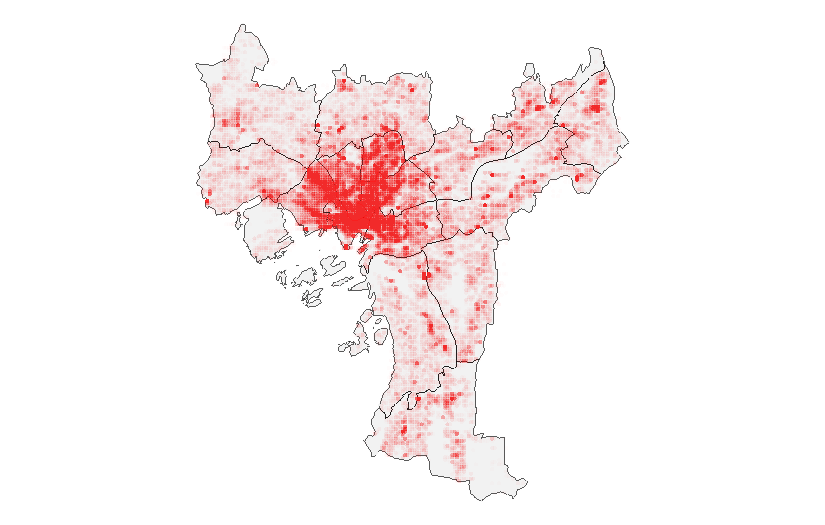
\includegraphics[keepaspectratio]{kart_files/figure-pdf/unnamed-chunk-25-1.pdf}}

Med \texttt{alpha\ =\ 0.01} (nesten gjennomsiktig) og
\texttt{size\ =\ 0.01} (sma punkter) kan vi vise alle hendelsene uten at
kartet blir helt rodt. Tettere omrader far sterkere farge fordi mange
halvgjennomsiktige punkter legges oppa hverandre.

\section{Rasterkart (heatmap)}\label{rasterkart-heatmap}

Punktkartet over er nyttig for a se det overordnede monsteret, men for a
sammenligne omrader mer presist trenger vi a \emph{aggregere} dataene.
Siden koordinatene allerede er avrundet til 100-meters ruter, kan vi
telle antall hendelser per rute:

\begin{Shaded}
\begin{Highlighting}[]
\NormalTok{krimplot }\OtherTok{\textless{}{-}}\NormalTok{ krim }\SpecialCharTok{\%\textgreater{}\%}
  \FunctionTok{group\_by}\NormalTok{(x, y) }\SpecialCharTok{\%\textgreater{}\%}
  \FunctionTok{summarise}\NormalTok{(}\AttributeTok{antall =} \FunctionTok{n}\NormalTok{()) }\SpecialCharTok{\%\textgreater{}\%}
  \FunctionTok{mutate}\NormalTok{(}\AttributeTok{antall =} \FunctionTok{ifelse}\NormalTok{(antall }\SpecialCharTok{\textgreater{}=} \DecValTok{200}\NormalTok{, }\DecValTok{200}\NormalTok{, antall))}
\end{Highlighting}
\end{Shaded}

Vi begrenser verdiene til maksimalt 200 for a unnga at noen ekstremt
tette ruter (typisk sentrum) dominerer hele fargeskalaen.

Na kan vi lage et rasterkart der hver rute er fargelagt etter antall
hendelser:

\begin{Shaded}
\begin{Highlighting}[]
\FunctionTok{ggplot}\NormalTok{(krimplot, }\FunctionTok{aes}\NormalTok{(}\AttributeTok{x =}\NormalTok{ x, }\AttributeTok{y =}\NormalTok{ y, }\AttributeTok{fill =}\NormalTok{ antall)) }\SpecialCharTok{+}
  \FunctionTok{geom\_tile}\NormalTok{() }\SpecialCharTok{+}
  \FunctionTok{coord\_sf}\NormalTok{(}\AttributeTok{datum =} \FunctionTok{st\_crs}\NormalTok{(oslo)) }\SpecialCharTok{+}
  \FunctionTok{theme\_void}\NormalTok{() }\SpecialCharTok{+}
  \FunctionTok{scale\_fill\_distiller}\NormalTok{(}\AttributeTok{palette =} \StringTok{"Spectral"}\NormalTok{)}
\end{Highlighting}
\end{Shaded}

\pandocbounded{\includegraphics[keepaspectratio]{kart_files/figure-pdf/unnamed-chunk-27-1.pdf}}

\texttt{geom\_tile()} tegner en firkant per rute, fargelagt etter antall
hendelser. \texttt{scale\_fill\_distiller(palette\ =\ "Spectral")} gir
en fargeskala som gar fra blatt (fa hendelser) til rodt (mange
hendelser).

For bedre kontekst legger vi til Oslos omriss oppa heatmapen:

\begin{Shaded}
\begin{Highlighting}[]
\NormalTok{oslo\_omkr }\OtherTok{\textless{}{-}} \FunctionTok{st\_union}\NormalTok{(oslo)}

\NormalTok{kart }\SpecialCharTok{+}
  \FunctionTok{geom\_tile}\NormalTok{(}\AttributeTok{data =}\NormalTok{ krimplot, }\FunctionTok{aes}\NormalTok{(}\AttributeTok{x =}\NormalTok{ x, }\AttributeTok{y =}\NormalTok{ y, }\AttributeTok{fill =}\NormalTok{ antall), }\AttributeTok{alpha =} \FloatTok{0.75}\NormalTok{) }\SpecialCharTok{+}
  \FunctionTok{scale\_fill\_distiller}\NormalTok{(}\AttributeTok{palette =} \StringTok{"Spectral"}\NormalTok{) }\SpecialCharTok{+}
  \FunctionTok{geom\_sf}\NormalTok{(}\AttributeTok{data =}\NormalTok{ oslo\_omkr, }\AttributeTok{color =} \StringTok{"black"}\NormalTok{, }\AttributeTok{fill =} \ConstantTok{NA}\NormalTok{) }\SpecialCharTok{+}
  \FunctionTok{labs}\NormalTok{(}\AttributeTok{fill =} \StringTok{"Hendelser"}\NormalTok{)}
\end{Highlighting}
\end{Shaded}

\pandocbounded{\includegraphics[keepaspectratio]{kart_files/figure-pdf/unnamed-chunk-28-1.pdf}}

\texttt{st\_union()} slar sammen alle bydelspolygonene til en ytre
grense. \texttt{fill\ =\ NA} gjor at bare grenselinjen tegnes, slik at
heatmapen synes gjennom. Merk at vi bruker grunnkartet (\texttt{kart})
som utgangspunkt og legger nye lag oppa -- akkurat samme prinsipp som
med vanlige ggplot-figurer.

\section{Oppdelt etter
kriminalitetstype}\label{oppdelt-etter-kriminalitetstype}

Med \texttt{facet\_wrap()} kan vi lage ett delkart per
kriminalitetstype. Vi aggregerer pa nytt, men na ogsa gruppert etter
type:

\begin{Shaded}
\begin{Highlighting}[]
\NormalTok{krimplot\_type }\OtherTok{\textless{}{-}}\NormalTok{ krim }\SpecialCharTok{\%\textgreater{}\%}
  \FunctionTok{group\_by}\NormalTok{(x, y, krimtypekodenavn) }\SpecialCharTok{\%\textgreater{}\%}
  \FunctionTok{summarise}\NormalTok{(}\AttributeTok{antall =} \FunctionTok{n}\NormalTok{()) }\SpecialCharTok{\%\textgreater{}\%}
  \FunctionTok{mutate}\NormalTok{(}\AttributeTok{antall =} \FunctionTok{ifelse}\NormalTok{(antall }\SpecialCharTok{\textgreater{}=} \DecValTok{150}\NormalTok{, }\DecValTok{150}\NormalTok{, antall))}

\NormalTok{kart }\SpecialCharTok{+}
  \FunctionTok{geom\_tile}\NormalTok{(}\AttributeTok{data =}\NormalTok{ krimplot\_type, }\FunctionTok{aes}\NormalTok{(}\AttributeTok{x =}\NormalTok{ x, }\AttributeTok{y =}\NormalTok{ y, }\AttributeTok{fill =}\NormalTok{ antall), }\AttributeTok{alpha =} \FloatTok{0.75}\NormalTok{) }\SpecialCharTok{+}
  \FunctionTok{scale\_fill\_distiller}\NormalTok{(}\AttributeTok{palette =} \StringTok{"Spectral"}\NormalTok{) }\SpecialCharTok{+}
  \FunctionTok{geom\_sf}\NormalTok{(}\AttributeTok{data =}\NormalTok{ oslo\_omkr, }\AttributeTok{color =} \StringTok{"black"}\NormalTok{, }\AttributeTok{fill =} \ConstantTok{NA}\NormalTok{) }\SpecialCharTok{+}
  \FunctionTok{facet\_wrap}\NormalTok{(}\SpecialCharTok{\textasciitilde{}}\NormalTok{krimtypekodenavn) }\SpecialCharTok{+}
  \FunctionTok{labs}\NormalTok{(}\AttributeTok{fill =} \StringTok{"Hendelser"}\NormalTok{)}
\end{Highlighting}
\end{Shaded}

\pandocbounded{\includegraphics[keepaspectratio]{kart_files/figure-pdf/unnamed-chunk-29-1.pdf}}

Na ser vi at de ulike kriminalitetstypene har svart forskjellig
geografisk fordeling. Vinningskriminalitet er spredt over hele byen,
mens narkotika er mer konsentrert. \texttt{facet\_wrap()} fungerer pa
kart akkurat som pa vanlige ggplot-figurer.

\section{Oppsummering}\label{oppsummering-1}

Kart i R folger samme logikk som annen ggplot-grafikk: du har data, du
velger en geometrisk form (\texttt{geom\_sf()}), og du tilpasser
utseendet. Med \texttt{sf}-pakken kan du lese inn kartfiler, koble pa
dine egne data, og lage bade statiske og interaktive kart. De viktigste
funksjonene a huske er:

\begin{longtable}[]{@{}ll@{}}
\toprule\noalign{}
Funksjon & Hva den gjor \\
\midrule\noalign{}
\endhead
\bottomrule\noalign{}
\endlastfoot
\texttt{st\_read()} & Leser inn geografiske data \\
\texttt{geom\_sf()} & Plotter sf-objekter i ggplot \\
\texttt{st\_as\_sf()} & Gjor vanlig data.frame om til sf-objekt \\
\texttt{st\_transform()} & Endrer koordinatreferansesystem \\
\texttt{st\_crs()} & Sjekker koordinatreferansesystemet \\
\texttt{st\_union()} & Slar sammen geometrier til en \\
\texttt{geom\_tile()} & Tegner rasterkart (heatmap) \\
\texttt{facet\_wrap()} & Deler kartet opp etter en variabel \\
\end{longtable}

\chapter{Nettverksanalyse}\label{nettverksanalyse}

\begin{Shaded}
\begin{Highlighting}[]
\FunctionTok{library}\NormalTok{(tidyverse)}
\FunctionTok{library}\NormalTok{(igraph)}
\end{Highlighting}
\end{Shaded}

Nettverksanalyse handler om relasjoner mellom enheter. Mens vi i
regresjonsanalyse fokuserer på egenskaper ved individer (f.eks. alder,
inntekt, utdanning), fokuserer nettverksanalyse på \emph{forbindelsene}
mellom dem. Hvem kjenner hvem? Hvem samarbeider med hvem? Hvilke
organisasjoner har overlappende styremedlemmer? Dette er typiske
sporsmal som nettverksanalyse kan belyse.

\section{Hva er et nettverk?}\label{hva-er-et-nettverk}

Et nettverk bestar av to grunnleggende byggeklosser: \emph{noder} og
\emph{kanter}. Nodene er enhetene i nettverket (f.eks. personer,
organisasjoner, land), mens kantene er forbindelsene mellom dem (f.eks.
vennskap, handelsrelasjoner, kommunikasjon).

I samfunnsvitenskap er vi ofte interessert i \emph{sosiale nettverk},
der nodene er personer og kantene representerer en eller annen form for
relasjon. Men nettverksanalyse brukes ogsa pa mange andre typer data.

\section{Typer nettverk}\label{typer-nettverk}

Det finnes ulike typer nettverk, og det er viktig a vite hvilken type
man jobber med:

\begin{itemize}
\tightlist
\item
  \textbf{Urettet nettverk}: Kantene gar begge veier. Vennskap er et
  typisk eksempel: hvis A er venn med B, sa er B venn med A.
\item
  \textbf{Rettet nettverk}: Kantene har en retning. Twitter-folging er
  et eksempel: A kan folge B uten at B folger A tilbake.
\item
  \textbf{Vektet nettverk}: Kantene har en styrke. F.eks. kan man vekte
  etter hvor mange ganger to personer har kommunisert.
\end{itemize}

\section{Lage nettverksobjekter med
igraph}\label{lage-nettverksobjekter-med-igraph}

Pakken \texttt{igraph} er det mest brukte verktøyet for nettverksanalyse
i R. La oss starte med a lage et lite eksempelnettverk. Tenk deg en
liten vennegjeng:

\begin{Shaded}
\begin{Highlighting}[]
\NormalTok{venner }\OtherTok{\textless{}{-}} \FunctionTok{graph\_from\_literal}\NormalTok{(Anna }\SpecialCharTok{{-}{-}}\NormalTok{ Bjorn,}
\NormalTok{                             Anna }\SpecialCharTok{{-}{-}}\NormalTok{ Cecilie,}
\NormalTok{                             Bjorn }\SpecialCharTok{{-}{-}}\NormalTok{ Cecilie,}
\NormalTok{                             Bjorn }\SpecialCharTok{{-}{-}}\NormalTok{ David,}
\NormalTok{                             Cecilie }\SpecialCharTok{{-}{-}}\NormalTok{ Elin,}
\NormalTok{                             David }\SpecialCharTok{{-}{-}}\NormalTok{ Elin,}
\NormalTok{                             David }\SpecialCharTok{{-}{-}}\NormalTok{ Fredrik)}
\NormalTok{venner}
\end{Highlighting}
\end{Shaded}

\begin{verbatim}
IGRAPH 2621013 UN-- 6 7 -- 
+ attr: name (v/c)
+ edges from 2621013 (vertex names):
[1] Anna   --Bjorn   Anna   --Cecilie Bjorn  --Cecilie Bjorn  --David  
[5] Cecilie--Elin    David  --Elin    David  --Fredrik
\end{verbatim}

Her har vi laget et urettet nettverk med seks personer og syv
relasjoner. Dobbel bindestrek \texttt{-\/-} betyr urettet kant. Hadde vi
brukt \texttt{+-+} ville det blitt rettet.

Vi kan plotte dette med en gang:

\begin{Shaded}
\begin{Highlighting}[]
\FunctionTok{plot}\NormalTok{(venner,}
     \AttributeTok{vertex.color =} \StringTok{"lightblue"}\NormalTok{,}
     \AttributeTok{vertex.size =} \DecValTok{30}\NormalTok{,}
     \AttributeTok{vertex.label.cex =} \FloatTok{0.9}\NormalTok{,}
     \AttributeTok{edge.color =} \StringTok{"gray50"}\NormalTok{,}
     \AttributeTok{main =} \StringTok{"Vennenettverket"}\NormalTok{)}
\end{Highlighting}
\end{Shaded}

\pandocbounded{\includegraphics[keepaspectratio]{nettverksanalyse_files/figure-pdf/unnamed-chunk-4-1.pdf}}

\section{Kantlister og nabomatriser}\label{kantlister-og-nabomatriser}

I praksis lager man sjelden nettverk for hand slik som ovenfor. Data
kommer ofte som en \emph{kantliste} (edge list), som er en tabell med to
kolonner: fra-node og til-node. Hver rad representerer en forbindelse
mellom to noder.

La oss lese inn det samme vennenettverket fra en CSV-fil:

\begin{Shaded}
\begin{Highlighting}[]
\NormalTok{kantliste }\OtherTok{\textless{}{-}} \FunctionTok{read\_csv}\NormalTok{(}\StringTok{"data/venner\_kantliste.csv"}\NormalTok{)}
\end{Highlighting}
\end{Shaded}

La oss se pa datastrukturen:

\begin{Shaded}
\begin{Highlighting}[]
\NormalTok{kantliste}
\end{Highlighting}
\end{Shaded}

\begin{verbatim}
# A tibble: 7 x 2
  fra     til    
  <chr>   <chr>  
1 Anna    Bjorn  
2 Anna    Cecilie
3 Bjorn   Cecilie
4 Bjorn   David  
5 Cecilie Elin   
6 David   Elin   
7 David   Fredrik
\end{verbatim}

Kantlisten er en helt vanlig tabell med to kolonner: \texttt{fra} og
\texttt{til}. Hver rad er en kant i nettverket. Dette er den vanligste
maten a lagre nettverksdata pa, og formatet er lett a lage i Excel eller
eksportere fra andre systemer.

Fra en slik kantliste kan vi lage et nettverksobjekt:

\begin{Shaded}
\begin{Highlighting}[]
\NormalTok{g }\OtherTok{\textless{}{-}} \FunctionTok{graph\_from\_data\_frame}\NormalTok{(kantliste, }\AttributeTok{directed =} \ConstantTok{FALSE}\NormalTok{)}
\FunctionTok{plot}\NormalTok{(g,}
     \AttributeTok{vertex.color =} \StringTok{"lightblue"}\NormalTok{,}
     \AttributeTok{vertex.size =} \DecValTok{30}\NormalTok{,}
     \AttributeTok{vertex.label.cex =} \FloatTok{0.9}\NormalTok{)}
\end{Highlighting}
\end{Shaded}

\pandocbounded{\includegraphics[keepaspectratio]{nettverksanalyse_files/figure-pdf/unnamed-chunk-7-1.pdf}}

En annen vanlig representasjon er en \emph{nabomatrise} (adjacency
matrix), der radene og kolonnene er noder, og cellene angir om det er en
kant mellom dem (1) eller ikke (0):

\begin{Shaded}
\begin{Highlighting}[]
\FunctionTok{as\_adjacency\_matrix}\NormalTok{(g, }\AttributeTok{sparse =} \ConstantTok{FALSE}\NormalTok{)}
\end{Highlighting}
\end{Shaded}

\begin{verbatim}
        Anna Bjorn Cecilie David Elin Fredrik
Anna       0     1       1     0    0       0
Bjorn      1     0       1     1    0       0
Cecilie    1     1       0     0    1       0
David      0     1       0     0    1       1
Elin       0     0       1     1    0       0
Fredrik    0     0       0     1    0       0
\end{verbatim}

Nabomatrisen er symmetrisk fordi nettverket er urettet. For rettede
nettverk ville matrisen typisk ikke vaert symmetrisk.

\section{Nettverksmaal}\label{nettverksmaal}

Nettverksanalyse tilbyr en rekke mal for a beskrive bade hele nettverket
og enkeltnoders posisjon. Her ser vi pa tre av de mest sentrale:

\subsection{Grad (degree)}\label{grad-degree}

Grad er det enkleste malet: hvor mange kanter har en node? I et
vennskapsnettverk betyr det rett og slett hvor mange venner en person
har.

\begin{Shaded}
\begin{Highlighting}[]
\FunctionTok{degree}\NormalTok{(g)}
\end{Highlighting}
\end{Shaded}

\begin{verbatim}
   Anna   Bjorn Cecilie   David    Elin Fredrik 
      2       3       3       3       2       1 
\end{verbatim}

Bjorn og David har flest forbindelser, mens Fredrik bare har en.

\subsection{Mellomleddsentralitet
(betweenness)}\label{mellomleddsentralitet-betweenness}

Mellomleddsentralitet maler hvor ofte en node ligger pa den korteste
veien mellom andre noder. En person med hay mellomleddsentralitet
fungerer som en \emph{bro} i nettverket.

\begin{Shaded}
\begin{Highlighting}[]
\FunctionTok{betweenness}\NormalTok{(g)}
\end{Highlighting}
\end{Shaded}

\begin{verbatim}
   Anna   Bjorn Cecilie   David    Elin Fredrik 
    0.0     3.0     1.5     4.5     1.0     0.0 
\end{verbatim}

\subsection{Naerhetssentralitet
(closeness)}\label{naerhetssentralitet-closeness}

Naerhetssentralitet maler hvor naer en node er alle andre noder i
nettverket. En person med hay naerhetssentralitet kan na alle andre
raskt.

\begin{Shaded}
\begin{Highlighting}[]
\FunctionTok{closeness}\NormalTok{(g)}
\end{Highlighting}
\end{Shaded}

\begin{verbatim}
      Anna      Bjorn    Cecilie      David       Elin    Fredrik 
0.11111111 0.14285714 0.12500000 0.14285714 0.12500000 0.09090909 
\end{verbatim}

La oss samle disse malene i en tabell:

\begin{Shaded}
\begin{Highlighting}[]
\NormalTok{sentralitet }\OtherTok{\textless{}{-}} \FunctionTok{tibble}\NormalTok{(}
  \AttributeTok{navn =} \FunctionTok{V}\NormalTok{(g)}\SpecialCharTok{$}\NormalTok{name,}
  \AttributeTok{grad =} \FunctionTok{degree}\NormalTok{(g),}
  \AttributeTok{mellomled =} \FunctionTok{round}\NormalTok{(}\FunctionTok{betweenness}\NormalTok{(g), }\DecValTok{1}\NormalTok{),}
  \AttributeTok{naerhet =} \FunctionTok{round}\NormalTok{(}\FunctionTok{closeness}\NormalTok{(g), }\DecValTok{3}\NormalTok{)}
\NormalTok{)}
\NormalTok{sentralitet}
\end{Highlighting}
\end{Shaded}

\begin{verbatim}
# A tibble: 6 x 4
  navn     grad mellomled naerhet
  <chr>   <dbl>     <dbl>   <dbl>
1 Anna        2       0     0.111
2 Bjorn       3       3     0.143
3 Cecilie     3       1.5   0.125
4 David       3       4.5   0.143
5 Elin        2       1     0.125
6 Fredrik     1       0     0.091
\end{verbatim}

Vi ser at Bjorn og David skiller seg ut som de mest sentrale personene i
dette nettverket, uansett hvilket mal vi bruker.

\section{Visualisering med ggraph}\label{visualisering-med-ggraph}

For finere grafisk kontroll kan vi bruke pakken \texttt{ggraph}, som
bygger pa ggplot-logikken:

\begin{Shaded}
\begin{Highlighting}[]
\FunctionTok{library}\NormalTok{(ggraph)}

\FunctionTok{ggraph}\NormalTok{(g, }\AttributeTok{layout =} \StringTok{"fr"}\NormalTok{) }\SpecialCharTok{+}
  \FunctionTok{geom\_edge\_link}\NormalTok{(}\AttributeTok{color =} \StringTok{"gray60"}\NormalTok{) }\SpecialCharTok{+}
  \FunctionTok{geom\_node\_point}\NormalTok{(}\AttributeTok{size =} \DecValTok{8}\NormalTok{, }\AttributeTok{color =} \StringTok{"steelblue"}\NormalTok{) }\SpecialCharTok{+}
  \FunctionTok{geom\_node\_text}\NormalTok{(}\FunctionTok{aes}\NormalTok{(}\AttributeTok{label =}\NormalTok{ name), }\AttributeTok{repel =} \ConstantTok{TRUE}\NormalTok{, }\AttributeTok{size =} \DecValTok{4}\NormalTok{) }\SpecialCharTok{+}
  \FunctionTok{theme\_void}\NormalTok{() }\SpecialCharTok{+}
  \FunctionTok{ggtitle}\NormalTok{(}\StringTok{"Vennenettverket med ggraph"}\NormalTok{)}
\end{Highlighting}
\end{Shaded}

\pandocbounded{\includegraphics[keepaspectratio]{nettverksanalyse_files/figure-pdf/unnamed-chunk-13-1.pdf}}

Her bruker vi Fruchterman-Reingold-algoritmen (\texttt{layout\ =\ "fr"})
for a plassere nodene. \texttt{geom\_edge\_link()} tegner kantene,
\texttt{geom\_node\_point()} tegner nodene, og
\texttt{geom\_node\_text()} legger pa navnene. Merk at dette folger
ggplot-logikken med lag oppå lag.

Vi kan ogsa la nodestorrelsen reflektere grad:

\begin{Shaded}
\begin{Highlighting}[]
\FunctionTok{ggraph}\NormalTok{(g, }\AttributeTok{layout =} \StringTok{"fr"}\NormalTok{) }\SpecialCharTok{+}
  \FunctionTok{geom\_edge\_link}\NormalTok{(}\AttributeTok{color =} \StringTok{"gray60"}\NormalTok{) }\SpecialCharTok{+}
  \FunctionTok{geom\_node\_point}\NormalTok{(}\FunctionTok{aes}\NormalTok{(}\AttributeTok{size =} \FunctionTok{degree}\NormalTok{(g)), }\AttributeTok{color =} \StringTok{"steelblue"}\NormalTok{) }\SpecialCharTok{+}
  \FunctionTok{geom\_node\_text}\NormalTok{(}\FunctionTok{aes}\NormalTok{(}\AttributeTok{label =}\NormalTok{ name), }\AttributeTok{repel =} \ConstantTok{TRUE}\NormalTok{, }\AttributeTok{size =} \DecValTok{4}\NormalTok{) }\SpecialCharTok{+}
  \FunctionTok{scale\_size\_continuous}\NormalTok{(}\AttributeTok{range =} \FunctionTok{c}\NormalTok{(}\DecValTok{4}\NormalTok{, }\DecValTok{12}\NormalTok{), }\AttributeTok{name =} \StringTok{"Grad"}\NormalTok{) }\SpecialCharTok{+}
  \FunctionTok{theme\_void}\NormalTok{()}
\end{Highlighting}
\end{Shaded}

\pandocbounded{\includegraphics[keepaspectratio]{nettverksanalyse_files/figure-pdf/unnamed-chunk-14-1.pdf}}

\section{Samfunnsdeteksjon}\label{samfunnsdeteksjon}

En vanlig oppgave i nettverksanalyse er a identifisere \emph{grupper}
(communities/klynger) av noder som er tettere knyttet til hverandre enn
til resten av nettverket. Det finnes flere algoritmer for dette. Her
bruker vi en enkel metode:

\begin{Shaded}
\begin{Highlighting}[]
\NormalTok{grupper }\OtherTok{\textless{}{-}} \FunctionTok{cluster\_walktrap}\NormalTok{(g)}
\FunctionTok{membership}\NormalTok{(grupper)}
\end{Highlighting}
\end{Shaded}

\begin{verbatim}
   Anna   Bjorn Cecilie   David    Elin Fredrik 
      2       2       2       1       1       1 
\end{verbatim}

Vi kan fargelegge nettverket etter gruppemedlemskap:

\begin{Shaded}
\begin{Highlighting}[]
\FunctionTok{plot}\NormalTok{(grupper, g,}
     \AttributeTok{vertex.size =} \DecValTok{30}\NormalTok{,}
     \AttributeTok{vertex.label.cex =} \FloatTok{0.9}\NormalTok{,}
     \AttributeTok{main =} \StringTok{"Grupper i vennenettverket"}\NormalTok{)}
\end{Highlighting}
\end{Shaded}

\pandocbounded{\includegraphics[keepaspectratio]{nettverksanalyse_files/figure-pdf/unnamed-chunk-16-1.pdf}}

\section{Praktisk eksempel:
samarbeidsnettverk}\label{praktisk-eksempel-samarbeidsnettverk}

Tenk deg et forskningssamarbeid mellom ansatte pa et institutt. Vi leser
inn en kantliste der hver rad er et samarbeid mellom to forskere, og
kolonnen \texttt{antall\_artikler} angir hvor mange felles artikler de
har:

\begin{Shaded}
\begin{Highlighting}[]
\NormalTok{samarbeid }\OtherTok{\textless{}{-}} \FunctionTok{read\_csv}\NormalTok{(}\StringTok{"data/samarbeid\_kantliste.csv"}\NormalTok{)}
\end{Highlighting}
\end{Shaded}

La oss se pa datastrukturen:

\begin{Shaded}
\begin{Highlighting}[]
\NormalTok{samarbeid}
\end{Highlighting}
\end{Shaded}

\begin{verbatim}
# A tibble: 11 x 3
   forsker1 forsker2 antall_artikler
   <chr>    <chr>              <dbl>
 1 Ola      Kari                   5
 2 Ola      Per                    2
 3 Kari     Liv                    3
 4 Kari     Mona                   1
 5 Per      Jan                    4
 6 Liv      Jan                    6
 7 Liv      Mona                   2
 8 Liv      Ola                    1
 9 Jan      Mona                   3
10 Jan      Ola                    1
11 Mona     Per                    1
\end{verbatim}

Denne kantlisten har tre kolonner: \texttt{forsker1} og
\texttt{forsker2} angir hvem som samarbeider, mens
\texttt{antall\_artikler} er en vekt som sier noe om styrken pa
relasjonen. Slike vektede kantlister er svart vanlige i praksis.

Na kan vi lage et nettverksobjekt og bruke vektene:

\begin{Shaded}
\begin{Highlighting}[]
\NormalTok{g2 }\OtherTok{\textless{}{-}} \FunctionTok{graph\_from\_data\_frame}\NormalTok{(samarbeid, }\AttributeTok{directed =} \ConstantTok{FALSE}\NormalTok{)}
\FunctionTok{E}\NormalTok{(g2)}\SpecialCharTok{$}\NormalTok{weight }\OtherTok{\textless{}{-}}\NormalTok{ samarbeid}\SpecialCharTok{$}\NormalTok{antall\_artikler}

\FunctionTok{ggraph}\NormalTok{(g2, }\AttributeTok{layout =} \StringTok{"fr"}\NormalTok{) }\SpecialCharTok{+}
  \FunctionTok{geom\_edge\_link}\NormalTok{(}\FunctionTok{aes}\NormalTok{(}\AttributeTok{width =}\NormalTok{ weight), }\AttributeTok{alpha =} \FloatTok{0.6}\NormalTok{, }\AttributeTok{color =} \StringTok{"gray40"}\NormalTok{) }\SpecialCharTok{+}
  \FunctionTok{geom\_node\_point}\NormalTok{(}\FunctionTok{aes}\NormalTok{(}\AttributeTok{size =} \FunctionTok{degree}\NormalTok{(g2)), }\AttributeTok{color =} \StringTok{"tomato"}\NormalTok{) }\SpecialCharTok{+}
  \FunctionTok{geom\_node\_text}\NormalTok{(}\FunctionTok{aes}\NormalTok{(}\AttributeTok{label =}\NormalTok{ name), }\AttributeTok{repel =} \ConstantTok{TRUE}\NormalTok{, }\AttributeTok{size =} \DecValTok{4}\NormalTok{) }\SpecialCharTok{+}
  \FunctionTok{scale\_edge\_width\_continuous}\NormalTok{(}\AttributeTok{range =} \FunctionTok{c}\NormalTok{(}\FloatTok{0.5}\NormalTok{, }\DecValTok{3}\NormalTok{), }\AttributeTok{name =} \StringTok{"Artikler"}\NormalTok{) }\SpecialCharTok{+}
  \FunctionTok{scale\_size\_continuous}\NormalTok{(}\AttributeTok{range =} \FunctionTok{c}\NormalTok{(}\DecValTok{4}\NormalTok{, }\DecValTok{12}\NormalTok{), }\AttributeTok{name =} \StringTok{"Grad"}\NormalTok{) }\SpecialCharTok{+}
  \FunctionTok{theme\_void}\NormalTok{() }\SpecialCharTok{+}
  \FunctionTok{ggtitle}\NormalTok{(}\StringTok{"Samarbeidsnettverk"}\NormalTok{)}
\end{Highlighting}
\end{Shaded}

\pandocbounded{\includegraphics[keepaspectratio]{nettverksanalyse_files/figure-pdf/unnamed-chunk-19-1.pdf}}

Her ser vi at kanttykkelsen viser antall felles artikler, mens
nodestorrelsen viser antall samarbeidspartnere. Liv og Jan ser ut til a
vaere sentrale i dette nettverket.

\section{Nar er nettverksanalyse
nyttig?}\label{nar-er-nettverksanalyse-nyttig}

Nettverksanalyse er et godt valg nar:

\begin{itemize}
\tightlist
\item
  Du er interessert i \emph{relasjoner} mellom enheter, ikke bare
  egenskaper ved enhetene selv.
\item
  Du vil identifisere sentrale aktorer i et nettverk (f.eks.
  nøkkelpersoner i en organisasjon).
\item
  Du vil forstå hvordan informasjon eller innflytelse sprer seg.
\item
  Du vil finne grupper eller klynger i data.
\item
  Du vil studere strukturen i et sosialt system.
\end{itemize}

Nettverksanalyse er mye brukt i sosiologi, statsvitenskap, kriminologi,
folkehelse og mange andre fagfelt. Det er et kraftig verktoy for a
forstå sosiale strukturer som ikke lar seg fange med tradisjonelle
regresjonsmodeller.

\part{Del III: Statistisk modellering}

\chapter{Regresjon: Sammenheng mellom
variable}\label{regresjon-sammenheng-mellom-variable}

\begin{Shaded}
\begin{Highlighting}[]
\FunctionTok{library}\NormalTok{(tidyverse)}
\FunctionTok{library}\NormalTok{(gtsummary)}
\FunctionTok{library}\NormalTok{(modelsummary)}
\end{Highlighting}
\end{Shaded}

Vi skal her se på helt grunnleggende lineær regresjon med en og to
forklaringsvariable.

\section{Scatterplot}\label{scatterplot-1}

Bivariat regresjon beskriver sammenhengen mellom to variable. En
naturlig start er å se på et scatterplot. Her er en figur som viser
hvordan timelønn varierer med alder. I det nedenforstående er det brukt
jitter og gjennomsiktig farge for å håndtere overplotting.

I tillegg er det tegnet inn en linje som illustrerer \emph{trenden i
gjennomsnittlig lønn} med alder. Denne linjen skrår svakt oppover, som
altså betyr at gjennomsnittlig lønn øker noe med alder. Vi ser med det
blotte øyet at en rett linje ikke beskriver denne sammenhengen perfekt.
Først og fremst er det en stor variasjon rundt denne linjen, så det er
mye annet som påvirker lønna enn alder. Det er også verd å legge merke
til at i de yngste aldersgruppene er lønna en god del lavere - og
kanskje litt lavere i eldste aldersgrupper også. Så en rett linje er
kanskje ikke optimalt i utgangspunktet. Fordelen med en rett linje er at
vi kan si noe slikt som at ``gjennosmsnittslønna øker med x antall
kroner for hvert år eldre man blir''. Hvis linja er kurvlineær blir det
litt mer komplisert. Så et første poeng er at en slik linje er en
\emph{forenkling}, og det er en tilsiktet forenkling.

\begin{Shaded}
\begin{Highlighting}[]
\FunctionTok{ggplot}\NormalTok{(abu89, }\FunctionTok{aes}\NormalTok{(}\AttributeTok{x =}\NormalTok{age, }\AttributeTok{y =}\NormalTok{ time89))}\SpecialCharTok{+}
  \FunctionTok{geom\_jitter}\NormalTok{(}\AttributeTok{alpha =}\NormalTok{ .}\DecValTok{2}\NormalTok{)}\SpecialCharTok{+}
  \FunctionTok{geom\_smooth}\NormalTok{(}\AttributeTok{method =} \StringTok{"lm"}\NormalTok{, }\AttributeTok{se =} \ConstantTok{FALSE}\NormalTok{)}
\end{Highlighting}
\end{Shaded}

\pandocbounded{\includegraphics[keepaspectratio]{lineaer_regresjon_files/figure-pdf/unnamed-chunk-4-1.pdf}}

Det er en viss tendens til at lønnen øker med alder, men det er ikke
helt lett å si hvor mye. Poenget med lineær regresjon er å beskrive en
gjennomsnittlig trend.

\begin{Shaded}
\begin{Highlighting}[]
\FunctionTok{ggplot}\NormalTok{(abu89, }\FunctionTok{aes}\NormalTok{(}\AttributeTok{x =}\NormalTok{age, }\AttributeTok{y =}\NormalTok{ time89))}\SpecialCharTok{+}
  \FunctionTok{geom\_jitter}\NormalTok{(}\AttributeTok{alpha =}\NormalTok{ .}\DecValTok{2}\NormalTok{)}\SpecialCharTok{+}
  \FunctionTok{geom\_smooth}\NormalTok{(}\AttributeTok{method =} \StringTok{"lm"}\NormalTok{, }\AttributeTok{se =} \ConstantTok{FALSE}\NormalTok{)}
\end{Highlighting}
\end{Shaded}

\pandocbounded{\includegraphics[keepaspectratio]{lineaer_regresjon_files/figure-pdf/unnamed-chunk-5-1.pdf}}

Denne trendlinja er hva vi vanligvis kaller regresjonslinje.

\section{Regresjonslinja}\label{regresjonslinja}

Regresjonslinja kan beskrives med et \emph{stigningstall}, som sier hvor
bratt linjen er. Substansielt sett betyr det hvor mye utfallsvariabelen
(y-aksen) endres med økning i forklaringsvariabelen (x-aksen). I tillegg
trenger vi også vite hvor høyt/lavt linjen ligger.\footnote{Du kan jo
  tenke deg flere parallelle linjer i plottet ovenfor med samme
  stigningstall} Til det bruker vi startpunktet for linjen, der hvor
\(x\) har verdien 0. Dette må regnes ut, og det er akkurat dette
estimering av lineær regresjon gir oss.

Utregningen av regresjonslinja går vi ikke inn på her, men intuitivt
sett ønsker vi jo \emph{den beste linja} og ikke en hvilken som helst
omtrentlig linje. Datapunktene (de svarte punktene i grafen) er spredt
rundt linja, og avstanden mellom linje og punkt kalles
\emph{residualer}. Summen av disse residualene er grunnlaget for mål på
hvor godt regresjonslinja beskriver de faktiske dataene. Den beste linja
er definert som den som minimerer residualene. Det er dette som kalles
``minste kvadraters metode''.

I R estimeres regresjonsmodeller med funksjonen \texttt{lm}. Første
argument er en formel på formen
\texttt{utfallsvariabel\ \textasciitilde{}\ forklaringsvariabel}.
Rekkefølgen variablene oppgis i er altså viktig. Dernest må det
spesifiseres hvilket datasett som skal brukes med \texttt{data\ =}
.\footnote{Grunnen til det siste er at R kan ha flere datasett oppe
  samtidig, så R vet ikke nødvendigvis hvilket datasett du tenker på}

Legg alltid resultatene i et eget objekt med et navnt som er rimelig
enkelt å forstå hva er. I følgende kode legges resultatet i en nytt
objekt \texttt{lm\_est1}. Deretter bruker kan man hente ut de delene av
resultatet vi er interessert i. I aller første omgang er bare
interessert i regresjonslinjas konstantledd (startpunktet) og
stigningstall. Disse kaller vi vanligvis \emph{regresjonskoeffisienter}.
Det kan vi få ut ved å bruke funksjonen \texttt{coef}. (Vi kommer
tilbake til å se på de fulle resultatene senere, som vi oftest er
interessert i).

\begin{Shaded}
\begin{Highlighting}[]
\NormalTok{lm\_est1 }\OtherTok{\textless{}{-}} \FunctionTok{lm}\NormalTok{(time89 }\SpecialCharTok{\textasciitilde{}}\NormalTok{ age, }\AttributeTok{data =}\NormalTok{ abu89)}
\FunctionTok{coef}\NormalTok{(lm\_est1)}
\end{Highlighting}
\end{Shaded}

\begin{verbatim}
(Intercept)         age 
 71.1101883   0.4828415 
\end{verbatim}

Regresjonslingningen kan skrives på formel der \(\alpha\) er
konstantleddet og \(\beta\) er stigningstallet slik:

\[
\operatorname{time89} = \alpha + \beta_{1}(\operatorname{age}) + \epsilon
\]

Når vi setter inn de estimerte koeffisientene inn i ligningen får vi
følgende:

\[
\operatorname{\widehat{time89}} = 71.11 + 0.48(\operatorname{age})
\]

Tolkningen her er at gjennomsnittlig forskjell i timelønn mellom grupper
der aldersforskjellen er ett år er 0.48 kroner i favør av den eldre
gruppen.\footnote{Noen ganger sier man at gjennomsnittslønna øker med
  0.48 kroner for hvert år eldre man blir. Men det er ikke helt riktig,
  for dataene beskriver jo ikke individuell endringer over tid! Men hvis
  du synes det er lettere å tenke på det på den måten er det ok - men
  prøv å husk at det også er litt feil.} Merk enheten her:
stigningstallet tolkes på den skalaen utfallsvariabelen er på, i dette
tilfellet kroner. Det er også uttrykt endring ved at
forklaringsvariabelen endres med nøyaktig 1.

Vi sier gjerne at regresjonslinjen er \emph{estimert}, og det innebærer
at det er usikkerhet i estimatene. Vi kommer tilbake til dette, men en
vanligere output fra regresjonsmodeller er å bruke funksjonen
\texttt{summary}. Da får man med mye mer detaljer og output vil se ut
som følger:

\begin{Shaded}
\begin{Highlighting}[]
\FunctionTok{summary}\NormalTok{(lm\_est1)}
\end{Highlighting}
\end{Shaded}

\begin{verbatim}

Call:
lm(formula = time89 ~ age, data = abu89)

Residuals:
    Min      1Q  Median      3Q     Max 
-69.287 -19.131  -6.304  12.864 255.258 

Coefficients:
            Estimate Std. Error t value Pr(>|t|)    
(Intercept) 71.11019    1.62232   43.83   <2e-16 ***
age          0.48284    0.03926   12.30   <2e-16 ***
---
Signif. codes:  0 '***' 0.001 '**' 0.01 '*' 0.05 '.' 0.1 ' ' 1

Residual standard error: 29.73 on 3757 degrees of freedom
  (368 observations deleted due to missingness)
Multiple R-squared:  0.0387,    Adjusted R-squared:  0.03844 
F-statistic: 151.2 on 1 and 3757 DF,  p-value: < 2.2e-16
\end{verbatim}

\section{Dummy-variable}\label{dummy-variable}

Hvis en forklaringsvariabel har kun to verdier vil vi typisk gi den ene
kategorien verdien 0 og den andre kategorien 1. Dette kalles en «dummy
variabel» eller en «indikator variabel». For eksempel vil et datasett
ofte ha en variabel for kjønn med verdiene «Mann» og «Kvinne». Da kan vi
la mann få verdien 0 og kvinne verdien 1. Ofte vil man da gi variabelen
et navn som indikerer hvilken verdi som er 1. Så i dette eksempelet er
det hensiktsmessig å gi den nye variabelen navnet «Kvinne». I dette
eksempelet vil man også kunne si at variabelen er en «dummy for kvinne»
(altså: den kategorien som får verdien 1).

Det spiller ingen rolle hvilken kategori som får verdien 0 og 1. I dette
eksempelet kunne man like gjerne gjort det motsatt, og latt det være en
«dummy for mann». Da ville det være naturlig å kalle variabelen «mann» i
stedet for «kvinne». Som vi skal se nedenfor vil det bare påvirke
fortegnet når vi bruker variabelen i en regresjonsanalyse.

I datasettet abu89 er variabelen ``female'' en slik variabel som har
verdiene 0 eller 1, og der 0 betyr ``mann'' og 1 betyr ``kvinne''.

\begin{longtable}[]{@{}ll@{}}
\toprule\noalign{}
Kjønn & Female \\
\midrule\noalign{}
\endhead
\bottomrule\noalign{}
\endlastfoot
Mann & 0 \\
Kvinne & 1 \\
Kvinne & 1 \\
Mann & 0 \\
Kvinne & 1 \\
Kvinne & 1 \\
Kvinne & 1 \\
Mann & 0 \\
\end{longtable}

I R vil vi ofte ha slike variable som factor-variable. Da er variabelen
definert som kategorisk og selv om det er tekst-verdier i variabelen, så
vil R automatisk behandle den som om verdiene var 0 og 1 i estimeringen
av regresjonsmodellen.

\begin{Shaded}
\begin{Highlighting}[]
\FunctionTok{theme\_gtsummary\_mean\_sd}\NormalTok{()}
\NormalTok{abu89 }\SpecialCharTok{\%\textgreater{}\%} 
  \FunctionTok{select}\NormalTok{(female, time89) }\SpecialCharTok{\%\textgreater{}\%} 
  \FunctionTok{tbl\_summary}\NormalTok{(}\AttributeTok{by =}\NormalTok{ female) }
\end{Highlighting}
\end{Shaded}

\begin{table}
\fontsize{12.0pt}{14.0pt}\selectfont
\begin{tabular*}{\linewidth}{@{\extracolsep{\fill}}lcc}
\toprule
\textbf{Characteristic} & \textbf{0}  N = 2,193\textsuperscript{\textit{1}} & \textbf{1}  N = 1,934\textsuperscript{\textit{1}} \\ 
\midrule\addlinespace[2.5pt]
Gjennomsnittlig timelønn 1989 & 100 (32) & 79 (24) \\ 
    Unknown & 190 & 178 \\ 
\bottomrule
\end{tabular*}
\begin{minipage}{\linewidth}
\vspace{.05em}
\textsuperscript{\textit{1}}Mean (SD)\\
\end{minipage}
\end{table}

Vi ser altså at menn hadde i gjennomsnitt høyere timelønn enn kvinner,
nærmere bestemt 21 kroner mer. Dette kan vi også undersøke med lineær
regresjon som følger:

\begin{Shaded}
\begin{Highlighting}[]
\NormalTok{lm\_est\_i }\OtherTok{\textless{}{-}} \FunctionTok{lm}\NormalTok{(time89 }\SpecialCharTok{\textasciitilde{}}\NormalTok{ female , }\AttributeTok{data =}\NormalTok{ abu89)}

\FunctionTok{coef}\NormalTok{(lm\_est\_i)}
\end{Highlighting}
\end{Shaded}

\begin{verbatim}
(Intercept)      female 
   99.84382   -20.75229 
\end{verbatim}

Regresjonskoeffisenten for variabelen female uttrykker nettopp
differansen mellom menn og kvinner, som er 21 kroner. Husk at \(\beta\)
er hvor mye \(y\)-variabelen endres når man sammenligner
\(x\)-variabelen med akkurat 1 enhets forskjell. Her er mann 0 og
kvinner 1, så da er dette faktisk 1 enhets forskjell. Altså: når \(x\)
går fra 0 til 1, så reduseres \(y\) med 21. Derfor negativt fortegn.

I R vil vi ofte gjøre om kategoriske variable til såkalte
factor-variable. En factor-variabel vil håndtere kategoriske variable
som tekst, men med en underliggende numerisk verdi. Da kan man bruke
factor-variable i alle standard analysemetoder. I regresjon vil R
automatisk bruke den første kategorien som referansekategori.

Vi kan gjøre den samme analysen med kjønn som en factor variabel og få
de samme resultatene som ovenefor.

\begin{Shaded}
\begin{Highlighting}[]
\NormalTok{abu89 }\OtherTok{\textless{}{-}}\NormalTok{ abu89 }\SpecialCharTok{\%\textgreater{}\%}
  \FunctionTok{mutate}\NormalTok{(}\AttributeTok{sex =} \FunctionTok{factor}\NormalTok{(}\FunctionTok{ifelse}\NormalTok{(female }\SpecialCharTok{==} \DecValTok{1}\NormalTok{, }\StringTok{"Female"}\NormalTok{, }\StringTok{"Male"}\NormalTok{), }\AttributeTok{levels =} \FunctionTok{c}\NormalTok{(}\StringTok{"Male"}\NormalTok{, }\StringTok{"Female"}\NormalTok{))) }\SpecialCharTok{\%\textgreater{}\%} 
  \FunctionTok{filter}\NormalTok{(}\SpecialCharTok{!}\FunctionTok{is.na}\NormalTok{(time89))}

\NormalTok{lm\_est2 }\OtherTok{\textless{}{-}} \FunctionTok{lm}\NormalTok{(time89 }\SpecialCharTok{\textasciitilde{}}\NormalTok{ female , }\AttributeTok{data =}\NormalTok{ abu89)}

\FunctionTok{coef}\NormalTok{(lm\_est2)}
\end{Highlighting}
\end{Shaded}

\begin{verbatim}
(Intercept)      female 
   99.84382   -20.75229 
\end{verbatim}

\subsection{Dummy-variable med mer enn en
kategori}\label{dummy-variable-med-mer-enn-en-kategori}

Noen ganger har vi forklaringsvariable med flere enn to kategorier. Det
kan vi løse på en tilsvarende måte ved å lage flere dummy-variable. Et
eksempel kan være sosial klasse. I datasettet abu89 er det fem
kategorier.

En dummy-variabel har bare to kategorier: 0 og 1, men vi kan lage flere
dummy-variable. Vi kan lager en ny variabel «klasse II» som har verdien
1 hvis personen tilhører denne klassen og 0 ellers. Altså en dummy. Så
kan vi lage en ny variabel «Klasse III» som har verdien 1 hvis personen
tilhører denne klassen og 0 ellers. Slik kan man lage en dummy-variabel
for hver av kategoriene. Da har vi altså flere dummy-variable som til
sammen fanger opp informasjonen i den opprinnelige variabelen.

\begin{longtable}[]{@{}lllll@{}}
\toprule\noalign{}
Utdanning & Klasse II & Klasse III & Klasse V-VI & Klasse VII \\
\midrule\noalign{}
\endhead
\bottomrule\noalign{}
\endlastfoot
Klasse I & 0 & 0 & 0 & 0 \\
Klasse II & 1 & 0 & 0 & 0 \\
Klasse III & 0 & 1 & 0 & 0 \\
Klasse V-VI & 0 & 0 & 1 & 0 \\
Klasse VII & 0 & 0 & 0 & 1 \\
\end{longtable}

Merk at her er det ingen dummy for ``Klasse I''. Denne gruppen brukes
som referansekategori slik at estimatene for \emph{de andre} dummyene
blir tolkbare som forskjellen til denne referansekategorien. Mer om det
siden, men man kan velge å bruke en annen referansekategori hvis man
vil.

La oss først se på et plot. Her er det brukt en jitter-plot. Den røde
linjen viser endring i gjennomsnitt mellom de kategoriene. En
regresjonsanalyse vil gi slike estimater på differanser, men det er
enklest hvis alle endringene er i forhold til samme referansekategori.

\begin{Shaded}
\begin{Highlighting}[]
\FunctionTok{ggplot}\NormalTok{( abu89x, }\FunctionTok{aes}\NormalTok{(}\AttributeTok{x =}\NormalTok{klasse89, }\AttributeTok{y =}\NormalTok{ time89))}\SpecialCharTok{+}
  \FunctionTok{geom\_jitter}\NormalTok{(}\AttributeTok{alpha =}\NormalTok{ .}\DecValTok{3}\NormalTok{, }\AttributeTok{width =}\NormalTok{ .}\DecValTok{2}\NormalTok{)}\SpecialCharTok{+}
  \FunctionTok{geom\_point}\NormalTok{(}\FunctionTok{aes}\NormalTok{(}\AttributeTok{y=}\NormalTok{gr\_snitt), }\AttributeTok{col =} \StringTok{"red"}\NormalTok{, }\AttributeTok{size =} \DecValTok{3}\NormalTok{)}\SpecialCharTok{+}
  \CommentTok{\#geom\_hline(yintercept = mean(abu89x$time89, na.rm = TRUE))+}
  \FunctionTok{geom\_line}\NormalTok{(}\FunctionTok{aes}\NormalTok{(}\AttributeTok{x =} \FunctionTok{as.numeric}\NormalTok{(klasse89), }\AttributeTok{y =}\NormalTok{ smooth), }\AttributeTok{col =} \StringTok{"red"}\NormalTok{, }\AttributeTok{linewidth =} \DecValTok{1}\NormalTok{) }
\end{Highlighting}
\end{Shaded}

\pandocbounded{\includegraphics[keepaspectratio]{lineaer_regresjon_files/figure-pdf/unnamed-chunk-14-1.pdf}}

Den generelle regresjonsligningen skrives som \(y=a+bx\), der \(x\) er
forklaringsvariabelen. Regresjonskoeffisienten, \(b\), tolkes som hvor
forskjellen i gjennomsnittet på utfallsvariabelen, \(y\), mellom de som
er en enhets forskjell på \(x\)-variabelen.

Så kan vi kjøre en regresjon og få ut regresjonskoeffisientene på samme
måte som før. Akkurat her er \texttt{coef} lagt inn i en parentes for
\texttt{data.frame}, men det er bare for at det skal bli en pen kolonne.
Vi kommer altså tilbake til teknikker for penere output nedenfor.

\begin{Shaded}
\begin{Highlighting}[]
\NormalTok{est2 }\OtherTok{\textless{}{-}} \FunctionTok{lm}\NormalTok{(time89 }\SpecialCharTok{\textasciitilde{}}\NormalTok{ klasse89, }\AttributeTok{data =}\NormalTok{ abu89)  }
\FunctionTok{data.frame}\NormalTok{(}\FunctionTok{coef}\NormalTok{(est2)) }
\end{Highlighting}
\end{Shaded}

\begin{verbatim}
                                 coef.est2.
(Intercept)                       118.39851
klasse89II Nedre serviceklasse    -14.49078
klasse89III Rutinefunksjonærer    -42.89842
klasse89V-VI Faglærte arbeidere   -29.68788
klasse89VIIa Ufaglærte arbeidere  -36.95234
\end{verbatim}

Hvert estimat for kategori for klasse sammenlignes med \emph{den første
kategorien} (altså den som mangler): klasse I. Det betyr at klasse VII
(ufaglærte arbeidere) har en timelønn på -37 kroner mindre enn klasse I
(øvre serviceklasse). Mens klasse II (nedre serviceklasse) tjener -14.5
kroner mindre enn klasse I.

Forskjellen mellom andre grupper er således differansen mellom disse
estimatene. Altså: klasse VII tjener mindre enn klasse V-VI:
\(36.9 - 29.7 = 7.2\) kroner. Se på plottet over, så ser du at disse
tallene ser riktige ut.

\section{Flere variable}\label{flere-variable}

Det er ikke så ofte vi bruker regresjon med bare en forklaringsvariabel,
såklat ``enkel lineær regresjon''.\footnote{Det er selvsagt ingenting
  \emph{enkelt} med slike modeller utover at det finnes mer kompliserte
  varianter.} Langt mer vanlig er å bruke flere variable samtidig i det
vi kaller ``multippel regresjon''.\footnote{Noen kaller dette også for
  \emph{multivariat} regresjon, men det er tvetydig da det også kan bety
  modeller med flere utfallsvariable, som er noe ganske annet.} I
multippel regresjon kan man altså beskrive mer kompliserte mønstre i
dataene.

Vi fortsetter med eksempelet om lønn og alder, men utvider med en
dimensjon til, nemlig kjønn. La oss først se på kjønnsforskjellene i
gjennomsnittlig timelønn.

\begin{Shaded}
\begin{Highlighting}[]
\NormalTok{abu89 }\OtherTok{\textless{}{-}}\NormalTok{ abu89 }\SpecialCharTok{\%\textgreater{}\%}
  \FunctionTok{mutate}\NormalTok{(}\AttributeTok{sex =} \FunctionTok{factor}\NormalTok{(}\FunctionTok{ifelse}\NormalTok{(female }\SpecialCharTok{==} \DecValTok{1}\NormalTok{, }\StringTok{"Female"}\NormalTok{, }\StringTok{"Male"}\NormalTok{), }\AttributeTok{levels =} \FunctionTok{c}\NormalTok{(}\StringTok{"Male"}\NormalTok{, }\StringTok{"Female"}\NormalTok{))) }\SpecialCharTok{\%\textgreater{}\%} 
  \FunctionTok{filter}\NormalTok{(}\SpecialCharTok{!}\FunctionTok{is.na}\NormalTok{(time89))}

\NormalTok{abu89 }\SpecialCharTok{\%\textgreater{}\%} 
  \FunctionTok{select}\NormalTok{(sex, time89) }\SpecialCharTok{\%\textgreater{}\%} 
  \FunctionTok{tbl\_summary}\NormalTok{(}\AttributeTok{by =}\NormalTok{ sex) }
\end{Highlighting}
\end{Shaded}

\begin{table}
\fontsize{12.0pt}{14.0pt}\selectfont
\begin{tabular*}{\linewidth}{@{\extracolsep{\fill}}lcc}
\toprule
\textbf{Characteristic} & \textbf{Male}  N = 2,003\textsuperscript{\textit{1}} & \textbf{Female}  N = 1,756\textsuperscript{\textit{1}} \\ 
\midrule\addlinespace[2.5pt]
Gjennomsnittlig timelønn 1989 & 100 (32) & 79 (24) \\ 
\bottomrule
\end{tabular*}
\begin{minipage}{\linewidth}
\vspace{.05em}
\textsuperscript{\textit{1}}Mean (SD)\\
\end{minipage}
\end{table}

Vi ser altså at menn hadde i gjennomsnitt høyere timelønn enn kvinner,
nærmere bestemt 21 kroner mer. Dette kan vi også undersøke med lineær
regresjon som følger:

\begin{Shaded}
\begin{Highlighting}[]
\NormalTok{lm\_est2 }\OtherTok{\textless{}{-}} \FunctionTok{lm}\NormalTok{(time89 }\SpecialCharTok{\textasciitilde{}}\NormalTok{ sex , }\AttributeTok{data =}\NormalTok{ abu89)}

\FunctionTok{coef}\NormalTok{(lm\_est2)}
\end{Highlighting}
\end{Shaded}

\begin{verbatim}
(Intercept)   sexFemale 
   99.84382   -20.75229 
\end{verbatim}

Det er altså slik at koeffisienten, \(\beta\), gir den samme differansen
som en enkel sammenligning av to gjennomsnitt.

Vi har allerede sett på alder og lønn, så vi kan utvide dette til å
inkludere kjønn samtidig i et scatterplot.

Grafisk er det da greit å bruke farger og slik vise for menn og kvinner
for seg. I \texttt{ggplot} spesifiseres da \texttt{group\ =\ sex} og at
fargene skal settes etter sammen grupperingen \texttt{col\ =\ sex} slik:

\begin{Shaded}
\begin{Highlighting}[]
\FunctionTok{ggplot}\NormalTok{(abu89, }\FunctionTok{aes}\NormalTok{(}\AttributeTok{x =}\NormalTok{ age, }\AttributeTok{y =}\NormalTok{ time89, }\AttributeTok{group =}\NormalTok{ sex, }\AttributeTok{col =}\NormalTok{ sex)) }\SpecialCharTok{+}
  \FunctionTok{geom\_jitter}\NormalTok{(}\AttributeTok{alpha =}\NormalTok{ .}\DecValTok{4}\NormalTok{)}
\end{Highlighting}
\end{Shaded}

\pandocbounded{\includegraphics[keepaspectratio]{lineaer_regresjon_files/figure-pdf/unnamed-chunk-18-1.pdf}}

\begin{Shaded}
\begin{Highlighting}[]
\NormalTok{lm\_est3 }\OtherTok{\textless{}{-}} \FunctionTok{lm}\NormalTok{(time89 }\SpecialCharTok{\textasciitilde{}}\NormalTok{ sex }\SpecialCharTok{+}\NormalTok{ age, }\AttributeTok{data =}\NormalTok{ abu89)}

\FunctionTok{coef}\NormalTok{(lm\_est3)}
\end{Highlighting}
\end{Shaded}

\begin{verbatim}
(Intercept)   sexFemale         age 
 81.1014711 -20.6251051   0.4738042 
\end{verbatim}

\subsection{Interaksjonsledd}\label{interaksjonsledd}

Det kan tenkes at hvordan inntekten varierer med alder er
\emph{forskjellig} for menn og kvinner. I modellen ovenfor er det
derimot antatt at denne er \emph{lik}. Vi kan beskrive forskjellen i
aldersgradienten i inntekt mellom menn og kvinner ved å inkludere
interaksjonsledd (samspill) mellom kjønn og alder.

Dette gjør vi ved å spesifisere en regresjonslikning som følger:

\[
time89 = \alpha + \beta_{1}(age) + \beta_{2}(sex) + \beta_{3}(age \times sex)
\] Eller med andre ord: timelønn varierer med \emph{alder} og
\emph{kjønn}, og \emph{kombinasjonen} av disse. Merk hvordan dette
skrives i R:

\begin{Shaded}
\begin{Highlighting}[]
\NormalTok{lm\_est4 }\OtherTok{\textless{}{-}} \FunctionTok{lm}\NormalTok{(time89 }\SpecialCharTok{\textasciitilde{}}\NormalTok{ sex }\SpecialCharTok{+}\NormalTok{ age }\SpecialCharTok{+}\NormalTok{ sex }\SpecialCharTok{*}\NormalTok{ age, }\AttributeTok{data =}\NormalTok{ abu89)}

\FunctionTok{coef}\NormalTok{(lm\_est4)}
\end{Highlighting}
\end{Shaded}

\begin{verbatim}
  (Intercept)     sexFemale           age sexFemale:age 
   75.8535901    -9.9048054     0.6064699    -0.2719530 
\end{verbatim}

Merk nå at referansekategorien for kjønn er menn, så den estimerte
koeffisienten er for kvinner. Det betyr at i utregningen får menn
verdien 0 og kvinner får verdien 1. Sette man det inn i
regresjonslikningen for menn blir det da som følger:

\[
time89 = \alpha + \beta_{1}(age) + \beta_{2}\times 0 + \beta_{3}(age \times 0)
\] Siden alt som multipliseres med 0 blir 0 kan vi også skrive dette
som:

\[
time89 = \alpha + \beta_{1}(age) 
\] For kvinner skal det derimot multipliseres med 1 og vi får:

\[
time89 = \alpha + \beta_{1}(age) + \beta_{2}\times 1 + \beta_{3}(age \times 1)
\] Det som multipliseres med 1 endres jo ikke, så da kan det skrives
som:

\[
time89 = \alpha + \beta_{1}(age) + \beta_{2} + \beta_{3}(age)
\] Men siden vi har to termer for alder kan det forkortes til:

\[
time89 = \alpha + (\beta_{1} + \beta_{3})(age) + \beta_{2} 
\] Kortere sagt: forskjellen i stigningstallet mellom menn og kvinner er
\(\beta_{3}\). I det empiriske eksempelet over betyr det at timelønn
øker med alder for begge kjønn, men for kvinner øker det med 0.27 kroner
mindre per år sammenlignet med menn. Eller sagt motsatt: menns lønn øker
med 0.27 mer enn kvinner per år.

\section{Prediksjon}\label{prediksjon}

Lineær regresjon kan også brukes til \emph{prediksjon} selv om dette i
liten grad er hva samfunnsvitere bruker regresjonsmodeller til.
Vanligvis vil vi primært være interessert i å tolke
regresjonskoeffisientene som sammenligninger mellom grupper. Man kan si
at man da er opptatt av \emph{forklaringsvariablene}. Når man predikerer
er man derimot opptatt av \emph{utfallsvariabelen}. Hvis man skulle være
interessert i temaer som maskinlæring, vil dette være en god inngang til
det.\footnote{f.eks. Et introduksjonskurs i maskinlæring som
  \href{https://www.uio.no/studier/emner/sv/iss/SOS2901/index.html}{SOS2901}
  starter gjerne med nettopp prediksjon med lineær regresjon.}

\subsection{Regne ut forventet verdi}\label{regne-ut-forventet-verdi}

Merk at konstantleddet er tolkbart som forventet verdi på
utfallsvariabelen når alle andre prediktorer er null. I eksempelet
ovenfor med timelønn og klassetilhøringhet, er det altså ikke noen
koeffisient for klasse I. Gjennomsnittlig timelønn i klasse I er når de
andre dummyene er 0, altså 118.4 kroner. Gjennomsnittlig timelønn for
klasse II er tilsvarende 118.4 + (-14.49) = 103.9.

Hvis du skulle gjette timelønna til en person uten å vite noe annet enn
klasseposisjon ville det være fornuftig å gjette på gjennomsnittet for
denne klassen. Så vi kan bruke regresjonsmodeller til å regne ut
gjennomsnittslønn for gitte verdier av forklaringsvariable. I dette
eksempelet er det kanskje litt i overkant komplisert da vi jo også bare
kunne regnet ut gjennomsnittet per gruppe i en enkel tabell. Det ville
faktisk gitt akkurat samme resultat. Det er mer nyttig med kontinuerlige
variable og mer kompliserte modeller.

La oss se på regresjonsmodellen for hvordan timelønn varierer med alder
i stedet. Alder er kontinuerlig, så det er få personer på hvert
alderstrinn.

\begin{Shaded}
\begin{Highlighting}[]
\FunctionTok{coef}\NormalTok{(lm\_est1)}
\end{Highlighting}
\end{Shaded}

\begin{verbatim}
(Intercept)         age 
 71.1101883   0.4828415 
\end{verbatim}

Gjennomsnittlig timelønn ved 30 år vil da være 71.1 + 30 \(\times\) 0.5
= 86.1 kroner. Ved 35 år blir det tilsvarende 71.1 + 35 \(\times\) 0.5 =
88.6 kroner.

Dette kan vi altså regne ut for hånd, men man kan også bruke en
r-funksjon, nemlig \texttt{predict}. Denne funksjonen tar som argument
et regresjonsobjekt og en data.frame (altså et datasett eller
tilsvarende struktur) med samme variabelnavn som ble brukt i opprinnelig
regresjonsmodell.\footnote{Hvis man ikke spesifiserer data.frame brukes
  opprinnelige data og predikerer for hver person. Det kan man også
  gjøre for å f.eks. regne ut residualer, men vi gjør ikke det her nå.}

\subsection{Predikere for kontinuerlig
variabel}\label{predikere-for-kontinuerlig-variabel}

Koden nedenfor lager først et datasett med én variabel: alder med noen
verdier man er interessert i utregning for. Så bruker man
\texttt{mutate} til å lage en kolonne til med predikerte verdier.

\begin{Shaded}
\begin{Highlighting}[]
\NormalTok{nyedata }\OtherTok{\textless{}{-}} \FunctionTok{data.frame}\NormalTok{(}\AttributeTok{age =} \FunctionTok{c}\NormalTok{(}\DecValTok{17}\NormalTok{, }\DecValTok{20}\NormalTok{, }\DecValTok{30}\NormalTok{, }\DecValTok{40}\NormalTok{, }\DecValTok{50}\NormalTok{, }\DecValTok{60}\NormalTok{))}

\NormalTok{nyedata }\SpecialCharTok{\%\textgreater{}\%} 
  \FunctionTok{mutate}\NormalTok{(}\AttributeTok{pred =} \FunctionTok{predict}\NormalTok{(lm\_est1, }\AttributeTok{newdata =}\NormalTok{ nyedata))}
\end{Highlighting}
\end{Shaded}

\begin{verbatim}
  age      pred
1  17  79.31849
2  20  80.76702
3  30  85.59543
4  40  90.42385
5  50  95.25226
6  60 100.08068
\end{verbatim}

\subsection{Predikere kategorisk
variabel}\label{predikere-kategorisk-variabel}

Tilsvarende kan vi predikere for kategoriske variable slik som ble
benyttet i regresjonsmodellen for klasse. I det nye datasettet
spesifiseres f.eks. alle nivåene av en factor-variabel med funksjonen
\texttt{levels} og predikerer for disse.

\begin{Shaded}
\begin{Highlighting}[]
\NormalTok{nyedata }\OtherTok{\textless{}{-}} \FunctionTok{data.frame}\NormalTok{(}\AttributeTok{klasse89 =} \FunctionTok{levels}\NormalTok{(abu89}\SpecialCharTok{$}\NormalTok{klasse89))}

\NormalTok{nyedata }\SpecialCharTok{\%\textgreater{}\%} 
  \FunctionTok{mutate}\NormalTok{(}\AttributeTok{pred =} \FunctionTok{predict}\NormalTok{(est2, }\AttributeTok{newdata =}\NormalTok{ nyedata))}
\end{Highlighting}
\end{Shaded}

\begin{verbatim}
                  klasse89      pred
1     I Øvre serviceklasse 118.39851
2   II Nedre serviceklasse 103.90773
3   III Rutinefunksjonærer  75.50009
4  V-VI Faglærte arbeidere  88.71063
5 VIIa Ufaglærte arbeidere  81.44618
\end{verbatim}

\subsection{Predikere for multippel
regresjon}\label{predikere-for-multippel-regresjon}

Nytten av predict-funksjonen kommer mer til sin rett ved mer kompliserte
modeller. Her er et eksempel med flere variable:

Så kan vi regne ut estimert gjennomsnittlig verdi for de ulike
kombinasjonene av utvalgte verdier som følger:

\begin{Shaded}
\begin{Highlighting}[]
\NormalTok{nyedata }\OtherTok{\textless{}{-}} \FunctionTok{expand.grid}\NormalTok{(}\AttributeTok{age =} \DecValTok{30}\SpecialCharTok{:}\DecValTok{35}\NormalTok{, }
                      \AttributeTok{sex =} \FunctionTok{c}\NormalTok{(}\StringTok{"Female"}\NormalTok{, }\StringTok{"Male"}\NormalTok{))}
\NormalTok{nyedata }\SpecialCharTok{\%\textgreater{}\%} 
  \FunctionTok{mutate}\NormalTok{(}\AttributeTok{pred =} \FunctionTok{predict}\NormalTok{(lm\_est3, }\AttributeTok{newdata =}\NormalTok{ nyedata))}
\end{Highlighting}
\end{Shaded}

\begin{verbatim}
   age    sex     pred
1   30 Female 74.69049
2   31 Female 75.16429
3   32 Female 75.63810
4   33 Female 76.11190
5   34 Female 76.58571
6   35 Female 77.05951
7   30   Male 95.31560
8   31   Male 95.78940
9   32   Male 96.26320
10  33   Male 96.73701
11  34   Male 97.21081
12  35   Male 97.68462
\end{verbatim}

Funksjonen \texttt{predict} fungerer på tilsvarende måte uansett hvor
komplisert modellen måtte være. Men det kreves at det nye datasettet har
samme variabelnavn og variabeltype som i opprinnelige data.

\section{Pene tabeller og eksport til
fil}\label{pene-tabeller-og-eksport-til-fil}

Slik resultatene ser ut med bruk av \texttt{summary} er forsåvidt fint,
og du får den informasjonen du trenger. Men det er ikke særlig
presentabelt som ferdig produkt i en analyse. Du trenger typisk to ting:
1) Samle flere regresjonsmodeller i samme tabell, og 2) gjøre tabellene
penere og lettere å lese, og 3) eksportere til det
tekstbehandlingsprogrammet du bruker, typisk Microsoft Word.

R har en hel rekke funksjoner for dette. Det spiller egentlig ingen
rolle hvilke funksjoner du bruker da det er noe smak og behag her, så
det viktigste er at det fungerer rimelig greit for deg. Nedenfor
presenteres tre pakker for dette formålet. Velg én av dem. Hvis du ikke
har egne preferanser, så velg det første alternativet: \{modelsummary\}.
Alle disse funksjonene håndterer svært mange typer modeller, gir gode
muligheter for å ferdigstille tabellene fullstendig før eksport, og
eksporterer til de formatene som er mest aktuelle. De har også mer
avansert funksjonalitet som f.eks. å rapportere robuste standardfeil (av
forskjellig type) i stedet for vanlige standardfeil (dette er pensum på
SOS4020).

Vi vil som regel ha behov for å flytte resultatene over til et
tekstbehandlingsprogram. En strategi som går ut på ``klipp og lim''
eller skjermbilde etc er uaktuelt og må unngås for nærmest enhver
pris.\footnote{Hvis du blir tatt i å gjøre slikt vil faglærer sette fyr
  på datamaskinen din som straff.} Resultatene skal skrives til en fil
på en effektiv måte. Det er en fordel om tabellene da ser ganske ok ut i
utgangspunktet og du kan bruke samme prosedyre for å eksportere til
flere typer format hvis behovet skulle melde seg. Det er jo MS Word som
er viktigst for de fleste, mens de øvrige formatene nedenfor er for
spesielt interessert - men noen av dere vil kanskje bli det på et senere
tidspunkt. De viktigste formatene som er:

\begin{itemize}
\tightlist
\item
  MS Word - det vanligste tekstbehandlingsprogrammet som de aller fleste
  av dere bruker.
\item
  rtf - rikt tekstformat. Er et enklere format som fungerer på tvers av
  de fleste programmer. Kan brukes i Word også.
\item
  html - for websider
\item
  latex - for mer tekniske dokumenter, særlig hvis du har mye formler og
  stæsj
\item
  Markdown/Quarto - for dynamiske dokumenter med integrert R-kode og
  tekst, og kan eksportere ferdig dokument til alle ovennevnte
  formater\footnote{F.eks. dette dokumentet er skrevet i Quarto} Det som
  fungerer med Markdown fungerer også med Quarto for samme formål.
\end{itemize}

\subsection{\texorpdfstring{Alt 1: Bruke
\texttt{modelsummary()}}{Alt 1: Bruke modelsummary()}}\label{alt-1-bruke-modelsummary}

Eksporterer til bl.a. følgende formater: Word, rtf, html, latex,
markdown

Fordel: Gir pene og oversiktlige tabeller med enkel kode, og relativt
enkelt å modifisere videre. Eksporterer direkte til alle viktigste
formater. Kan også lett integreres med andre eksterne verktøy, først og
fremst ``grammar of tables'' i pakket \{gt\} Ulempe:

Her er kode for en enkel tabell med to regresjonsmodeller som vist
ovenfor. Merk at objektene med regresjonsresultatene må legges inni
funksjonen \texttt{list()}.

\begin{Shaded}
\begin{Highlighting}[]
\FunctionTok{library}\NormalTok{(modelsummary)}
\FunctionTok{modelsummary}\NormalTok{(}\FunctionTok{list}\NormalTok{(lm\_est2, lm\_est3))}
\end{Highlighting}
\end{Shaded}

\begin{table}
\centering
\begin{tblr}[         %% tabularray outer open
]                     %% tabularray outer close
{                     %% tabularray inner open
colspec={Q[]Q[]Q[]},
hline{2}={1-3}{solid, black, 0.05em},
hline{8}={1-3}{solid, black, 0.05em},
hline{1}={1-3}{solid, black, 0.08em},
hline{16}={1-3}{solid, black, 0.08em},
column{2-3}={}{halign=c},
column{1}={}{halign=l},
}                     %% tabularray inner close
& (1) & (2) \\
(Intercept) & \num{99.844} & \num{81.101} \\
& (\num{0.637}) & (\num{1.585}) \\
sexFemale & \num{-20.752} & \num{-20.625} \\
& (\num{0.932}) & (\num{0.912}) \\
age &  & \num{0.474} \\
&  & (\num{0.037}) \\
Num.Obs. & \num{3759} & \num{3759} \\
R2 & \num{0.117} & \num{0.154} \\
R2 Adj. & \num{0.116} & \num{0.153} \\
AIC & \num{35854.9} & \num{35694.9} \\
BIC & \num{35873.6} & \num{35719.8} \\
Log.Lik. & \num{-17924.434} & \num{-17843.437} \\
F & \num{496.278} & \num{341.699} \\
RMSE & \num{28.49} & \num{27.88} \\
\end{tblr}
\end{table}

Denne tabellen inneholder mer enn du er interessert i. Nedre del av
tabellen inneholder ``goodness of fit'' statistikker, altså mål på
hvordan modellen passer til dataene. Det finnes mange slike, men ingen
grunn til å gå seg vill i disse her. De kan fjernes med argumentet
\texttt{gof\_omit\ =} og så angis statistikkene med de navnene du ser i
tabellen. Det skrives på en spesiell måte: som en tekststreng angitt med
anførselstegn rundt, og \texttt{\textbar{}} mellom hver. I koden
nedenfor beholdes kun antall observasjoner, \(r^2\) og \(F\).\footnote{Øvrige
  statistikker har selvsagt sitt bruksområde. De nevnte holder for de
  fleste formål.}

Vi gjør et par andre justeringer samtidig for å demonstrere noe
funksjonalitet. I stedet for å oppgi estimatet og standardfeil på
forskjellig linje kan vi spesifisere å ha det på samme linje med
argumentet \texttt{estimate\ =}. Merk at den statistikken du vil
rapportere settes i parentes \{\ldots\} og mellomrom og parentes er
ellers som det står. Man har også andre valg, derav det vanligste i bruk
er å angi \emph{p}-verdier eller \emph{stjerner} for å vise disse på en
forenklet måte. Det angis ved \texttt{\{p.value\}} eller
\texttt{\{stars\}} på tilsvarende måte.

I stedet for standardfeil på egen linje er det her angitt
konfidensintervall på neste linje. For konfidensintervall vil det som
forvalg være 95\%, men vi kan angi f.eks. 99\% konfidensintervall i
stedet ved \texttt{conf\_level\ =}. Hvis man ikke vil ha noe på neste
linje kan man angi \texttt{statistic\ =\ NULL} i stedet. Man kan også
velge å sette inn \texttt{p.value} eller \texttt{stars} på denne linjen.

Merk at utfallsvariabelen i modellene er timelønn i kroner. I forrige
tabell ble estimatene gitt med tre desimaler. Det er i overkant mange
desimaler. En desimal er mer passende og nedenfor endres dette med
\texttt{fmt\ =}.

\begin{Shaded}
\begin{Highlighting}[]
\FunctionTok{modelsummary}\NormalTok{(}\FunctionTok{list}\NormalTok{(lm\_est2, lm\_est3), }
             \AttributeTok{fmt =} \DecValTok{1}\NormalTok{,}
             \AttributeTok{estimate =} \StringTok{"\{estimate\} (\{std.error\})"}\NormalTok{,}
             \AttributeTok{statistic =} \StringTok{\textquotesingle{}conf.int\textquotesingle{}}\NormalTok{, }
             \AttributeTok{conf\_level =}\NormalTok{ .}\DecValTok{99}\NormalTok{, }
             \AttributeTok{gof\_omit =} \StringTok{\textquotesingle{}DF|Deviance|R2 Adj.|AIC|BIC|Log.Lik.|RMSE\textquotesingle{}}\NormalTok{)}
\end{Highlighting}
\end{Shaded}

\begin{table}
\centering
\begin{tblr}[         %% tabularray outer open
]                     %% tabularray outer close
{                     %% tabularray inner open
colspec={Q[]Q[]Q[]},
hline{2}={1-3}{solid, black, 0.05em},
hline{8}={1-3}{solid, black, 0.05em},
hline{1}={1-3}{solid, black, 0.08em},
hline{11}={1-3}{solid, black, 0.08em},
column{2-3}={}{halign=c},
column{1}={}{halign=l},
}                     %% tabularray inner close
& (1) & (2) \\
(Intercept) & \num{99.8} (\num{0.6}) & \num{81.1} (\num{1.6}) \\
& [\num{98.2}, \num{101.5}] & [\num{77.0}, \num{85.2}] \\
sexFemale & \num{-20.8} (\num{0.9}) & \num{-20.6} (\num{0.9}) \\
& [\num{-23.2}, \num{-18.4}] & [\num{-23.0}, \num{-18.3}] \\
age &  & \num{0.5} (\num{0.0}) \\
&  & [\num{0.4}, \num{0.6}] \\
Num.Obs. & \num{3759} & \num{3759} \\
R2 & \num{0.117} & \num{0.154} \\
F & \num{496.278} & \num{341.699} \\
\end{tblr}
\end{table}

To siste ting å ta med her er å endre navn på variablene til noe mer
presentabelt og eksportere til Word. Med argumentet
\texttt{coef\_rename\ =} angis variabelen slik den ser ut i output og
spesifiserer hva du vil skal stå. Koden nedenfor viser eksempel.

For å eksportere til Word settes \texttt{output\ =} med filbane og
filnavn, og der filhalen \emph{.docx} angir Word format. Du kan
eksportere til annet format ved å angi annen filhale f.eks. .rtf eller
.html.

\begin{table}
\centering
\begin{tblr}[         %% tabularray outer open
]                     %% tabularray outer close
{                     %% tabularray inner open
colspec={Q[]Q[]Q[]},
hline{2}={1-3}{solid, black, 0.05em},
hline{8}={1-3}{solid, black, 0.05em},
hline{1}={1-3}{solid, black, 0.08em},
hline{11}={1-3}{solid, black, 0.08em},
column{2-3}={}{halign=c},
column{1}={}{halign=l},
}                     %% tabularray inner close
& (1) & (2) \\
Konstant & \num{99.8} (\num{0.6}) & \num{81.1} (\num{1.6}) \\
& [\num{98.2}, \num{101.5}] & [\num{77.0}, \num{85.2}] \\
Kvinne & \num{-20.8} (\num{0.9}) & \num{-20.6} (\num{0.9}) \\
& [\num{-23.2}, \num{-18.4}] & [\num{-23.0}, \num{-18.3}] \\
Alder &  & \num{0.5} (\num{0.0}) \\
&  & [\num{0.4}, \num{0.6}] \\
Num.Obs. & \num{3759} & \num{3759} \\
R2 & \num{0.117} & \num{0.154} \\
F & \num{496.278} & \num{341.699} \\
\end{tblr}
\end{table}

\begin{Shaded}
\begin{Highlighting}[]
\FunctionTok{modelsummary}\NormalTok{(}\FunctionTok{list}\NormalTok{(lm\_est2, lm\_est3), }
             \AttributeTok{fmt =} \DecValTok{1}\NormalTok{,}
             \AttributeTok{estimate =} \StringTok{"\{estimate\} (\{std.error\})"}\NormalTok{,}
             \AttributeTok{statistic =} \StringTok{\textquotesingle{}conf.int\textquotesingle{}}\NormalTok{, }
             \AttributeTok{conf\_level =}\NormalTok{ .}\DecValTok{99}\NormalTok{, }
             \AttributeTok{gof\_omit =} \StringTok{\textquotesingle{}DF|Deviance|R2 Adj.|AIC|BIC|Log.Lik.|RMSE\textquotesingle{}}\NormalTok{, }
             \AttributeTok{coef\_rename =} \FunctionTok{c}\NormalTok{(}\StringTok{"sexFemale"} \OtherTok{=} \StringTok{"Kvinne"}\NormalTok{, }
                                   \StringTok{"age"} \OtherTok{=} \StringTok{"Alder"}\NormalTok{, }
                                  \StringTok{"(Intercept)"} \OtherTok{=} \StringTok{"Konstant"}\NormalTok{), }
             \AttributeTok{output =} \StringTok{"output/reg\_table.docx"}\NormalTok{)}
\end{Highlighting}
\end{Shaded}

Merk at Word vil vise tabellen med de fonter etc som er forvalgt for
Word. Dette kan du endre i Word etterpå. Det er en rekke funksjoner i
Word for å formattere tabeller som du kan bruke.

Pakken \{modelsummary\} har også en rekke andre funksjoner for å
redigere tabeller som du kan utforske ved behov. For avanserte brukere
kan man også gjøre om tabellen til et gt-objekt og redigere videre med
pakken \{gt\} eller tilsvarende med pakken \{flextable\}. Det er altså
tilnærmet uendelige muligheter for avanserte tabeller. Dette går
imidlertid langt utenfor hva de fleste av dere vil trenge.
\{modelsummary\} har
\href{https://vincentarelbundock.github.io/modelsummary/index.html}{egen
hjemmeside} med mer detaljer og instruksjoner.

\subsection{Alt 2: Bruke \{stargazer\}}\label{alt-2-bruke-stargazer}

Mange R-brukere foretrekker pakken \{stargazer\}. Dette er en noe eldre
funksjon og er derfor godt etablert.

Eksporterer til bl.a. følgende formater: rtf, html, latex, markdown

Fordel: Er en stand-alone pakke men gir enkelt veldig fine tabeller som
antakeligvis er det du trenger Ulempe: Eksport til Word er ikke den
beste, men god nok.

Stargazer lager tabeller i kun tre formater: latex, html, og ren tekst.
Vi velger derfor \texttt{type\ =\ "text"} for at det skal se ok ut her.

\begin{Shaded}
\begin{Highlighting}[]
\FunctionTok{library}\NormalTok{(stargazer)}
\FunctionTok{stargazer}\NormalTok{(lm\_est2, lm\_est3, }\AttributeTok{type =} \StringTok{"text"}\NormalTok{)}
\end{Highlighting}
\end{Shaded}

\begin{verbatim}

=======================================================================
                                    Dependent variable:                
                    ---------------------------------------------------
                                          time89                       
                               (1)                       (2)           
-----------------------------------------------------------------------
sexFemale                  -20.752***                -20.625***        
                             (0.932)                   (0.912)         
                                                                       
age                                                   0.474***         
                                                       (0.037)         
                                                                       
Constant                    99.844***                 81.101***        
                             (0.637)                   (1.585)         
                                                                       
-----------------------------------------------------------------------
Observations                  3,759                     3,759          
R2                            0.117                     0.154          
Adjusted R2                   0.116                     0.153          
Residual Std. Error    28.495 (df = 3757)        27.891 (df = 3756)    
F Statistic         496.278*** (df = 1; 3757) 341.699*** (df = 2; 3756)
=======================================================================
Note:                                       *p<0.1; **p<0.05; ***p<0.01
\end{verbatim}

Vi kan modifisere tabellen tilsvarende som vi gjorde med
\{modelsummary\}. Forklaringer av de enkelte argumenter finnes i
\href{https://cran.r-project.org/web/packages/stargazer/stargazer.pdf}{manualen
for stargazer}.

\texttt{covariate.labels\ =} Angir teksten for variabelnavn. Merk at det
oppgis i den \emph{rekkefølgen} det skal stå, så være veldig nøye hvis
du har mange variable! \texttt{report\ =} angir hva som skal inngå i
tabellen, der hver bokstav viser til spesifikke deler: v = variabelnavn,
c = koeffisient/estimat, s = standardfeil. \texttt{single.row\ =} setter
statistikkene på samme linje fremfor under hverandre.
\texttt{keep.stat\ =} angir hvilke ``model fit statistics'' som skal
rapporteres. Hvis du skriver ``all'' her får du en lang remse
tilsvarende vi fikk med \{modelsummary\}. \texttt{digits\ =} angir
antall desimaler

\begin{Shaded}
\begin{Highlighting}[]
\FunctionTok{stargazer}\NormalTok{(lm\_est2, lm\_est3, }
          \AttributeTok{type =} \StringTok{"text"}\NormalTok{, }
          \AttributeTok{covariate.labels =} \FunctionTok{c}\NormalTok{(}\StringTok{"Kvinne"}\NormalTok{, }\StringTok{"Alder"}\NormalTok{, }\StringTok{"Konstant"}\NormalTok{),}
          \AttributeTok{report =} \StringTok{"vcs"}\NormalTok{,}
          \AttributeTok{single.row =} \ConstantTok{TRUE}\NormalTok{, }
          \AttributeTok{keep.stat =} \FunctionTok{c}\NormalTok{(}\StringTok{"n"}\NormalTok{,}\StringTok{"rsq"}\NormalTok{, }\StringTok{"ser"}\NormalTok{),}
          \AttributeTok{digits =} \DecValTok{1}\NormalTok{)}
\end{Highlighting}
\end{Shaded}

\begin{verbatim}

=====================================================
                           Dependent variable:       
                    ---------------------------------
                                 time89              
                          (1)              (2)       
-----------------------------------------------------
Kvinne                -20.8 (0.9)      -20.6 (0.9)   
Alder                                   0.5 (0.04)   
Konstant               99.8 (0.6)       81.1 (1.6)   
-----------------------------------------------------
Observations             3,759            3,759      
R2                        0.1              0.2       
Residual Std. Error 28.5 (df = 3757) 27.9 (df = 3756)
=====================================================
Note:                     *p<0.1; **p<0.05; ***p<0.01
\end{verbatim}

For å eksportere til Word kan man bruke rikt tekstformat (.rtf) eller
html. rtf-formatet er som navnet tilsier ren tekst og selv om det ser
greit ut, så er videre redigering i et tekstbehandlingsprogram krøkete.
(Prøv og se selv). Bruk heller html fordi da beholdes tabell-strukturen.
Du kan åpne html-tabeller fra Word og redigere videre der ved behov.

\begin{Shaded}
\begin{Highlighting}[]
\FunctionTok{stargazer}\NormalTok{(lm\_est2, lm\_est3, }
          \AttributeTok{type =} \StringTok{"text"}\NormalTok{,}
          \AttributeTok{covariate.labels =} \FunctionTok{c}\NormalTok{(}\StringTok{"Kvinne"}\NormalTok{, }\StringTok{"Alder"}\NormalTok{, }\StringTok{"Konstant"}\NormalTok{),}
          \AttributeTok{report =} \StringTok{"vcs"}\NormalTok{,}
          \AttributeTok{single.row =} \ConstantTok{TRUE}\NormalTok{, }
          \AttributeTok{keep.stat =} \FunctionTok{c}\NormalTok{(}\StringTok{"n"}\NormalTok{,}\StringTok{"rsq"}\NormalTok{, }\StringTok{"ser"}\NormalTok{),}
          \AttributeTok{digits =} \DecValTok{1}\NormalTok{, }
          \AttributeTok{out =} \StringTok{"output/reg\_starg.html"}\NormalTok{)}
\end{Highlighting}
\end{Shaded}

Mer detaljer finner du i
\href{https://cran.r-project.org/web/packages/stargazer/vignettes/stargazer.pdf}{\{stargazer\}
sin vignette}.

\subsection{Alt 3: Bruke \{gtsummary\}}\label{alt-3-bruke-gtsummary}

Vi har tidligere brukt \{gtsummary\} for å lage deskriptive tabeller,
som er det pakken er best til. Men den kan også lage gode
regresjonstabeller. Det er imidlertid en stor ulempe for nybegynnere i
R: det er ganske krøkete å sette sammen flere regresjonsmodeller i en
samlet tabell. Derfor er rådet å \emph{ikke bruke} denne pakken med
mindre du har veldig lyst til å prøve.

Fordel med å bruke denne pakken er at man slipper å lære enda en ny
pakke og slik sett ha ett sett med konsistent syntaks. En mulighet er
selvsagt å ikke lage tabellene så ferdig i R, men eksportere til Word og
redigere ferdig der mer manuelt.

\{gtsummary\} kan eksportere til følgende formater: Word, rtf, html,
latex og markdown. Resultatene kan også lett integreres med andre
funksjoner, først og fremst ``grammar of tables'' i pakket \{gt\} og
\{flextable\} - altså for mer avanserte ting som vi ikke dekker her.

Prinsippet er å lage hver tabell for seg og så slå dem sammen med
\texttt{tbl\_merge} etterpå. Det innebærer en del mer kode, rett og
slett. I utgangspunktet virker det ganske greit, men det er alltid en
del småting som krever litt mer.

Følgende kode lager først en ryddig tabell for hver regresionsmodell og
så kobler sammen disse to tabellene.

\begin{Shaded}
\begin{Highlighting}[]
\NormalTok{lm\_tab1 }\OtherTok{\textless{}{-}} \FunctionTok{tbl\_regression}\NormalTok{(lm\_est2, }\AttributeTok{intercept =}\NormalTok{ T, }
                          \AttributeTok{estimate\_fun =} \ControlFlowTok{function}\NormalTok{(x) }\FunctionTok{style\_number}\NormalTok{(x, }\AttributeTok{digits =} \DecValTok{1}\NormalTok{),}
                          \AttributeTok{show\_single\_row =} \StringTok{"sex"}\NormalTok{,}
                          \AttributeTok{label =} \FunctionTok{list}\NormalTok{(sex }\SpecialCharTok{\textasciitilde{}} \StringTok{"Kvinne"}\NormalTok{)) }\SpecialCharTok{\%\textgreater{}\%} 
    \FunctionTok{add\_glance\_table}\NormalTok{(}\AttributeTok{include =} \FunctionTok{c}\NormalTok{(nobs, r.squared, sigma))}
                     
\NormalTok{lm\_tab2 }\OtherTok{\textless{}{-}} \FunctionTok{tbl\_regression}\NormalTok{(lm\_est3, }\AttributeTok{intercept =}\NormalTok{ T,}
                          \AttributeTok{estimate\_fun =} \ControlFlowTok{function}\NormalTok{(x) }\FunctionTok{style\_number}\NormalTok{(x, }\AttributeTok{digits =} \DecValTok{1}\NormalTok{), }
                          \AttributeTok{show\_single\_row =} \StringTok{"sex"}\NormalTok{,}
                          \AttributeTok{label =} \FunctionTok{list}\NormalTok{(age }\SpecialCharTok{\textasciitilde{}} \StringTok{"Alder"}\NormalTok{, sex }\SpecialCharTok{\textasciitilde{}} \StringTok{"Kvinne"}\NormalTok{)) }\SpecialCharTok{\%\textgreater{}\%} 
    \FunctionTok{add\_glance\_table}\NormalTok{(}\AttributeTok{include =} \FunctionTok{c}\NormalTok{(nobs, r.squared, sigma)}
\NormalTok{  )}


\FunctionTok{tbl\_merge}\NormalTok{(}\AttributeTok{tbls =} \FunctionTok{list}\NormalTok{(lm\_tab1, lm\_tab2)) }\SpecialCharTok{\%\textgreater{}\%} 
  \FunctionTok{modify\_table\_body}\NormalTok{(}
    \SpecialCharTok{\textasciitilde{}}\NormalTok{.x }\SpecialCharTok{\%\textgreater{}\%} 
\NormalTok{      dplyr}\SpecialCharTok{::}\FunctionTok{arrange}\NormalTok{(}
\NormalTok{        row\_type }\SpecialCharTok{==} \StringTok{"glance\_statistic"}\NormalTok{, }\CommentTok{\# sort glance table to bottom}
\NormalTok{        var\_label                       }\CommentTok{\# sort by the variable label (a hidden column) }
\NormalTok{      )}
\NormalTok{  )}
\end{Highlighting}
\end{Shaded}

\begin{verbatim}
The number rows in the tables to be merged do not match, which may result in
rows appearing out of order.
i See `tbl_merge()` (`?gtsummary::tbl_merge()`) help file for details. Use
  `quiet=TRUE` to silence message.
\end{verbatim}

\begin{table}
\fontsize{12.0pt}{14.0pt}\selectfont
\begin{tabular*}{\linewidth}{@{\extracolsep{\fill}}lcccccc}
\toprule
 & \multicolumn{3}{c}{{\textbf{Table 1}}} & \multicolumn{3}{c}{{\textbf{Table 2}}} \\ 
\cmidrule(lr){2-4} \cmidrule(lr){5-7}
\textbf{Characteristic} & \textbf{Beta} & \textbf{95\% CI} & \textbf{p-value} & \textbf{Beta} & \textbf{95\% CI} & \textbf{p-value} \\ 
\midrule\addlinespace[2.5pt]
(Intercept) & 99.8 & 98.6, 101.1 & <0.001 & 81.1 & 78.0, 84.2 & <0.001 \\ 
Alder &  &  &  & 0.5 & 0.4, 0.5 & <0.001 \\ 
Kvinne & -20.8 & -22.6, -18.9 & <0.001 & -20.6 & -22.4, -18.8 & <0.001 \\ 
{No. Obs.} & {3,759} & {} & {} & {3,759} & {} & {} \\ 
R² & 0.117 &  &  & 0.154 &  &  \\ 
Sigma & 28.5 &  &  & 27.9 &  &  \\ 
\bottomrule
\end{tabular*}
\begin{minipage}{\linewidth}
\vspace{.05em}
Abbreviation: CI = Confidence Interval\\
\end{minipage}
\end{table}

\chapter{Utvidelser av
regresjonsmodeller}\label{utvidelser-av-regresjonsmodeller}

\begin{Shaded}
\begin{Highlighting}[]
\FunctionTok{library}\NormalTok{(tidyverse)}
\FunctionTok{library}\NormalTok{(haven)}
\FunctionTok{library}\NormalTok{(modelsummary)}
\FunctionTok{library}\NormalTok{(lmtest)}
\FunctionTok{library}\NormalTok{(sandwich)}
\end{Highlighting}
\end{Shaded}

I forrige kapittel så vi på helt grunnleggende lineær regresjon. Det er
et godt utgangspunkt, men i praksis trenger man ofte å utvide modellene
litt. I dette kapittelet ser vi på noen av de vanligste utvidelsene:
ikke-lineære sammenhenger, log-transformasjoner, og robuste
standardfeil. Alt dette er ting du vil møte i pensumlitteraturen og i
empiriske artikler, så det er nyttig å vite hvordan det gjøres i R.

\section{Polynomiske ledd: ikke-lineære
sammenhenger}\label{polynomiske-ledd-ikke-lineuxe6re-sammenhenger}

I forrige kapittel så vi at sammenhengen mellom alder og timelønn ikke
nødvendigvis er helt lineær. Kanskje lønna øker raskt i starten av
karrieren, flater ut, og så synker litt mot slutten? En rett linje
fanger ikke opp dette. En enkel løsning er å legge til et
\emph{andregradsledd}, altså alder i andre potens (\(alder^2\)). Da får
vi en kurve i stedet for en rett linje.

I R bruker vi funksjonen \texttt{poly()} eller legger til
\texttt{I(age\^{}2)} direkte i formelen. La oss prøve begge:

\begin{Shaded}
\begin{Highlighting}[]
\NormalTok{est\_lin }\OtherTok{\textless{}{-}} \FunctionTok{lm}\NormalTok{(time89 }\SpecialCharTok{\textasciitilde{}}\NormalTok{ age, }\AttributeTok{data =}\NormalTok{ abu89)}
\NormalTok{est\_poly }\OtherTok{\textless{}{-}} \FunctionTok{lm}\NormalTok{(time89 }\SpecialCharTok{\textasciitilde{}}\NormalTok{ age }\SpecialCharTok{+} \FunctionTok{I}\NormalTok{(age}\SpecialCharTok{\^{}}\DecValTok{2}\NormalTok{), }\AttributeTok{data =}\NormalTok{ abu89)}
\end{Highlighting}
\end{Shaded}

La oss sammenligne de to modellene:

\begin{Shaded}
\begin{Highlighting}[]
\FunctionTok{modelsummary}\NormalTok{(}\FunctionTok{list}\NormalTok{(}\StringTok{"Lineær"} \OtherTok{=}\NormalTok{ est\_lin, }\StringTok{"Kvadratisk"} \OtherTok{=}\NormalTok{ est\_poly),}
             \AttributeTok{fmt =} \DecValTok{2}\NormalTok{,}
             \AttributeTok{gof\_omit =} \StringTok{\textquotesingle{}DF|Deviance|AIC|BIC|Log.Lik.|RMSE\textquotesingle{}}\NormalTok{)}
\end{Highlighting}
\end{Shaded}

\begin{table}
\centering
\begin{tblr}[         %% tabularray outer open
]                     %% tabularray outer close
{                     %% tabularray inner open
colspec={Q[]Q[]Q[]},
hline{2}={1-3}{solid, black, 0.05em},
hline{8}={1-3}{solid, black, 0.05em},
hline{1}={1-3}{solid, black, 0.08em},
hline{12}={1-3}{solid, black, 0.08em},
column{2-3}={}{halign=c},
column{1}={}{halign=l},
}                     %% tabularray inner close
& Lineær & Kvadratisk \\
(Intercept) & \num{71.11} & \num{5.11} \\
& (\num{1.62}) & (\num{4.60}) \\
age & \num{0.48} & \num{4.01} \\
& (\num{0.04}) & (\num{0.23}) \\
I(age\textasciicircum{}2) &  & \num{-0.04} \\
&  & (\num{0.00}) \\
Num.Obs. & \num{3759} & \num{3759} \\
R2 & \num{0.039} & \num{0.095} \\
R2 Adj. & \num{0.038} & \num{0.094} \\
F & \num{151.239} & \num{197.015} \\
\end{tblr}
\end{table}

Koeffisienten for \texttt{I(age\^{}2)} er negativ, noe som betyr at
kurven bøyer nedover. Altså: lønna øker med alder, men økningen avtar.
Dette gir en omvendt U-form som er ganske typisk for inntekt over
livsløpet.

Merk at når du har med et andregradsledd er det ikke lenger meningsfylt
å tolke koeffisienten for \texttt{age} alene. De to koeffisientene må
tolkes \emph{sammen} fordi de beskriver ulike deler av den samme kurven.
Den beste måten å forstå effekten på er å se på et plot:

\begin{Shaded}
\begin{Highlighting}[]
\FunctionTok{ggplot}\NormalTok{(abu89, }\FunctionTok{aes}\NormalTok{(}\AttributeTok{x =}\NormalTok{ age, }\AttributeTok{y =}\NormalTok{ time89)) }\SpecialCharTok{+}
  \FunctionTok{geom\_jitter}\NormalTok{(}\AttributeTok{alpha =}\NormalTok{ .}\DecValTok{15}\NormalTok{) }\SpecialCharTok{+}
  \FunctionTok{geom\_smooth}\NormalTok{(}\AttributeTok{method =} \StringTok{"lm"}\NormalTok{, }\AttributeTok{formula =}\NormalTok{ y }\SpecialCharTok{\textasciitilde{}}\NormalTok{ x,}
              \AttributeTok{se =} \ConstantTok{FALSE}\NormalTok{, }\AttributeTok{col =} \StringTok{"blue"}\NormalTok{, }\AttributeTok{linetype =} \StringTok{"dashed"}\NormalTok{) }\SpecialCharTok{+}
  \FunctionTok{geom\_smooth}\NormalTok{(}\AttributeTok{method =} \StringTok{"lm"}\NormalTok{, }\AttributeTok{formula =}\NormalTok{ y }\SpecialCharTok{\textasciitilde{}}\NormalTok{ x }\SpecialCharTok{+} \FunctionTok{I}\NormalTok{(x}\SpecialCharTok{\^{}}\DecValTok{2}\NormalTok{),}
              \AttributeTok{se =} \ConstantTok{FALSE}\NormalTok{, }\AttributeTok{col =} \StringTok{"red"}\NormalTok{) }\SpecialCharTok{+}
  \FunctionTok{labs}\NormalTok{(}\AttributeTok{x =} \StringTok{"Alder"}\NormalTok{, }\AttributeTok{y =} \StringTok{"Timelønn (kr)"}\NormalTok{) }\SpecialCharTok{+}
  \FunctionTok{theme\_minimal}\NormalTok{()}
\end{Highlighting}
\end{Shaded}

\pandocbounded{\includegraphics[keepaspectratio]{regresjon_utvidelser_files/figure-pdf/unnamed-chunk-6-1.pdf}}

Den stiplete blå linjen er den lineære modellen, mens den røde kurven er
modellen med andregradsledd. Vi ser at den røde kurven fanger opp
mønsteret i dataene bedre, særlig for de yngste og de eldste.

Man kan i prinsippet legge til høyere ordens ledd (\texttt{I(age\^{}3)}
osv.), men i praksis er det sjelden nødvendig med mer enn
andregradsledd. Høyere ordens polynomer gir fort rare kurver som er
vanskelige å tolke og som gjerne bare tilpasser seg støy i dataene.

\section{Log-transformasjoner}\label{log-transformasjoner}

En annen vanlig måte å håndtere ikke-lineære sammenhenger på er å bruke
\emph{logaritmen} av variablene. Dette er særlig nyttig for variable som
inntekt, lønn, og andre økonomiske størrelser som ofte har en skjev
fordeling med en lang hale til høyre.

\subsection{Logaritme av
utfallsvariabelen}\label{logaritme-av-utfallsvariabelen}

Hvis vi tar logaritmen av utfallsvariabelen (\texttt{time89}), endrer vi
tolkningen av koeffisientene. Nå uttrykkes endringer i \emph{prosent} i
stedet for i kroner:

\begin{Shaded}
\begin{Highlighting}[]
\NormalTok{est\_log }\OtherTok{\textless{}{-}} \FunctionTok{lm}\NormalTok{(}\FunctionTok{log}\NormalTok{(time89) }\SpecialCharTok{\textasciitilde{}}\NormalTok{ age, }\AttributeTok{data =}\NormalTok{ abu89)}

\FunctionTok{modelsummary}\NormalTok{(}\FunctionTok{list}\NormalTok{(}\StringTok{"Kroner"} \OtherTok{=}\NormalTok{ est\_lin, }\StringTok{"Log(kroner)"} \OtherTok{=}\NormalTok{ est\_log),}
             \AttributeTok{fmt =} \DecValTok{3}\NormalTok{,}
             \AttributeTok{gof\_omit =} \StringTok{\textquotesingle{}DF|Deviance|AIC|BIC|Log.Lik.|RMSE\textquotesingle{}}\NormalTok{)}
\end{Highlighting}
\end{Shaded}

\begin{table}
\centering
\begin{tblr}[         %% tabularray outer open
]                     %% tabularray outer close
{                     %% tabularray inner open
colspec={Q[]Q[]Q[]},
hline{2}={1-3}{solid, black, 0.05em},
hline{6}={1-3}{solid, black, 0.05em},
hline{1}={1-3}{solid, black, 0.08em},
hline{10}={1-3}{solid, black, 0.08em},
column{2-3}={}{halign=c},
column{1}={}{halign=l},
}                     %% tabularray inner close
& Kroner & Log(kroner) \\
(Intercept) & \num{71.110} & \num{4.226} \\
& (\num{1.622}) & (\num{0.016}) \\
age & \num{0.483} & \num{0.006} \\
& (\num{0.039}) & (\num{0.000}) \\
Num.Obs. & \num{3759} & \num{3759} \\
R2 & \num{0.039} & \num{0.053} \\
R2 Adj. & \num{0.038} & \num{0.053} \\
F & \num{151.239} & \num{210.357} \\
\end{tblr}
\end{table}

I den første modellen (i kroner) betyr koeffisienten for alder at
timelønna øker med ca. 0.48 \emph{kroner} per år. I den andre modellen
(log) betyr koeffisienten at timelønna øker med ca. 0.5\% per
år.\footnote{Teknisk sett er tolkningen at en enhets økning i alder er
  assosiert med en endring i log-timelønn på 0.005. For å få
  prosent-tolkning multipliserer man med 100. Denne tilnærmingen
  fungerer godt for små koeffisienter (under ca. 0.1), men for større
  koeffisienter bør man bruke den eksakte formelen:
  \((e^\beta - 1) \times 100\).}

\subsection{Logaritme av
forklaringsvariabelen}\label{logaritme-av-forklaringsvariabelen}

Man kan også ta logaritmen av forklaringsvariabelen. Da endres
tolkningen til å handle om \emph{prosentvis} endring i
forklaringsvariabelen. Vi bruker et annet eksempel her fordi log av
alder ikke er så meningsfylt, men log av f.eks. arbeidstid eller
lignende variable kan gi mening i andre datasett.

\subsection{Oppsummering av
log-transformasjoner}\label{oppsummering-av-log-transformasjoner}

\begin{longtable}[]{@{}
  >{\raggedright\arraybackslash}p{(\linewidth - 2\tabcolsep) * \real{0.2759}}
  >{\raggedright\arraybackslash}p{(\linewidth - 2\tabcolsep) * \real{0.7241}}@{}}
\toprule\noalign{}
\begin{minipage}[b]{\linewidth}\raggedright
Modell
\end{minipage} & \begin{minipage}[b]{\linewidth}\raggedright
Tolkning av \(\beta\)
\end{minipage} \\
\midrule\noalign{}
\endhead
\bottomrule\noalign{}
\endlastfoot
\(y = \alpha + \beta x\) & \(x\) opp 1 enhet \(\rightarrow\) \(y\)
endres med \(\beta\) enheter \\
\(\log(y) = \alpha + \beta x\) & \(x\) opp 1 enhet \(\rightarrow\) \(y\)
endres med ca. \(\beta \times 100\) prosent \\
\(y = \alpha + \beta \log(x)\) & \(x\) opp 1\% \(\rightarrow\) \(y\)
endres med ca. \(\beta / 100\) enheter \\
\(\log(y) = \alpha + \beta \log(x)\) & \(x\) opp 1\% \(\rightarrow\)
\(y\) endres med ca. \(\beta\) prosent (elastisitet) \\
\end{longtable}

Denne tabellen er verd å ha i bakhodet. Det siste tilfellet, der begge
er log-transformert, er det man kaller en \emph{elastisitet} i økonomi.

\section{Robuste standardfeil}\label{robuste-standardfeil}

Standardfeilene fra vanlig OLS-regresjon bygger på en antakelse om at
variansen i feilleddene er \emph{konstant} (homoskedastisitet). Hvis
denne antakelsen er brutt -- noe den ofte er i praksis -- kan
standardfeilene bli feil. Konsekvensen er at konfidensintervaller og
p-verdier ikke er til å stole på.

Løsningen er å bruke \emph{robuste standardfeil}, gjerne kalt
``Huber-White'' eller ``sandwich'' standardfeil. Disse gir korrekte
standardfeil selv om variansen ikke er konstant.\footnote{Det som endres
  er altså bare standardfeilene og dermed p-verdier og
  konfidensintervaller. Selve koeffisientene (estimatene) er de samme.}

\subsection{\texorpdfstring{Med
\texttt{modelsummary}}{Med modelsummary}}\label{med-modelsummary}

Den enkleste måten å rapportere robuste standardfeil i R er å bruke
\texttt{vcov}-argumentet i \texttt{modelsummary}. Da trenger du ikke
engang å laste ekstra pakker utover det du allerede har:

\begin{Shaded}
\begin{Highlighting}[]
\FunctionTok{modelsummary}\NormalTok{(}\FunctionTok{list}\NormalTok{(}\StringTok{"Vanlige SE"} \OtherTok{=}\NormalTok{ est\_lin, }\StringTok{"Robuste SE"} \OtherTok{=}\NormalTok{ est\_lin),}
             \AttributeTok{vcov =} \FunctionTok{list}\NormalTok{(}\StringTok{"classical"}\NormalTok{, }\StringTok{"HC1"}\NormalTok{),}
             \AttributeTok{fmt =} \DecValTok{2}\NormalTok{,}
             \AttributeTok{gof\_omit =} \StringTok{\textquotesingle{}DF|Deviance|AIC|BIC|Log.Lik.|RMSE\textquotesingle{}}\NormalTok{)}
\end{Highlighting}
\end{Shaded}

\begin{table}
\centering
\begin{tblr}[         %% tabularray outer open
]                     %% tabularray outer close
{                     %% tabularray inner open
colspec={Q[]Q[]Q[]},
hline{2}={1-3}{solid, black, 0.05em},
hline{6}={1-3}{solid, black, 0.05em},
hline{1}={1-3}{solid, black, 0.08em},
hline{11}={1-3}{solid, black, 0.08em},
column{2-3}={}{halign=c},
column{1}={}{halign=l},
}                     %% tabularray inner close
& Vanlige SE & Robuste SE \\
(Intercept) & \num{71.11} & \num{71.11} \\
& (\num{1.62}) & (\num{1.52}) \\
age & \num{0.48} & \num{0.48} \\
& (\num{0.04}) & (\num{0.04}) \\
Num.Obs. & \num{3759} & \num{3759} \\
R2 & \num{0.039} & \num{0.039} \\
R2 Adj. & \num{0.038} & \num{0.038} \\
F & \num{151.239} & \num{155.345} \\
Std.Errors & Classical & HC1 \\
\end{tblr}
\end{table}

Her er det nøyaktig \emph{samme} modell i begge kolonnene, men med ulike
standardfeil. \texttt{"HC1"} er den vanligste varianten av robuste
standardfeil og tilsvarer det Stata bruker som forvalg.\footnote{Det
  finnes flere varianter: HC0, HC1, HC2, HC3. HC1 er den mest brukte i
  praksis og inkluderer en korreksjon for antall observasjoner.}

\subsection{\texorpdfstring{Med \texttt{lmtest} og
\texttt{sandwich}}{Med lmtest og sandwich}}\label{med-lmtest-og-sandwich}

Du kan også bruke pakkene \texttt{lmtest} og \texttt{sandwich} direkte
for å se robuste standardfeil:

\begin{Shaded}
\begin{Highlighting}[]
\FunctionTok{coeftest}\NormalTok{(est\_lin, }\AttributeTok{vcov =} \FunctionTok{vcovHC}\NormalTok{(est\_lin, }\AttributeTok{type =} \StringTok{"HC1"}\NormalTok{))}
\end{Highlighting}
\end{Shaded}

\begin{verbatim}

t test of coefficients:

            Estimate Std. Error t value  Pr(>|t|)    
(Intercept) 71.11019    1.51953  46.797 < 2.2e-16 ***
age          0.48284    0.03874  12.464 < 2.2e-16 ***
---
Signif. codes:  0 '***' 0.001 '**' 0.01 '*' 0.05 '.' 0.1 ' ' 1
\end{verbatim}

Dette gir deg koeffisientene, robuste standardfeil, t-verdier og
p-verdier. Funksjonen \texttt{vcovHC} beregner den robuste
varians-kovariansmatrisen, og \texttt{coeftest} bruker denne til å
beregne nye teststatistikker.

\section{Klustrede standardfeil}\label{klustrede-standardfeil}

I noen datasett er observasjonene gruppert, f.eks. elever innenfor
skoler, eller ansatte innenfor bedrifter. Da kan observasjoner innenfor
samme gruppe være mer like hverandre enn observasjoner på tvers av
grupper. Vanlige standardfeil tar ikke hensyn til dette og kan bli for
\emph{lave}, noe som gjør at man feilaktig finner ``statistisk
signifikante'' resultater.

Løsningen er \emph{klustrede standardfeil}, som tar hensyn til
gruppestrukturen. I \texttt{modelsummary} kan dette gjøres med
\texttt{vcov}-argumentet ved å angi en formel med klustervariabelen:

\begin{Shaded}
\begin{Highlighting}[]
\FunctionTok{modelsummary}\NormalTok{(}\FunctionTok{list}\NormalTok{(est\_lin),}
             \AttributeTok{vcov =} \SpecialCharTok{\textasciitilde{}}\NormalTok{klasse89,}
             \AttributeTok{fmt =} \DecValTok{2}\NormalTok{)}
\end{Highlighting}
\end{Shaded}

Klustrede standardfeil er særlig viktig i paneldata og flernivådata. Vi
går ikke dypere inn på dette her, men det er viktig å vite at det finnes
og at det er enkelt å implementere.

\section{Vektet regresjon}\label{vektet-regresjon}

Noen ganger har vi data der observasjonene har ulik \emph{vekt}. Det kan
for eksempel være at noen observasjoner er mer pålitelige enn andre,
eller at datasettet er et stratifisert utvalg der noen grupper er
overrepresentert. I slike tilfeller bruker vi \emph{vektet regresjon}.

I R legger man til \texttt{weights}-argumentet i \texttt{lm}:

\begin{Shaded}
\begin{Highlighting}[]
\NormalTok{est\_vektet }\OtherTok{\textless{}{-}} \FunctionTok{lm}\NormalTok{(time89 }\SpecialCharTok{\textasciitilde{}}\NormalTok{ age }\SpecialCharTok{+}\NormalTok{ female, }\AttributeTok{data =}\NormalTok{ abu89, }\AttributeTok{weights =}\NormalTok{ en\_vekt\_variabel)}
\end{Highlighting}
\end{Shaded}

Vektet regresjon er vanlig i analyser av surveydata der ulike grupper
har ulik trekkesannsynlighet. Mange norske datasett fra SSB kommer med
slike vekter. Prinsippet er at observasjoner med høyere vekt teller mer
i estimeringen.

\section{Faste effekter (fixed
effects)}\label{faste-effekter-fixed-effects}

Faste effekter er en teknikk som brukes mye i paneldata, altså data der
man observerer de samme enhetene over flere tidspunkter. Ideen er å
kontrollere for \emph{alle} tidskonstante egenskaper ved enhetene, også
de man ikke har observert. For eksempel: hvis man ser på lønnsutvikling
over tid, vil faste effekter for person fjerne all variasjon som skyldes
uobserverte, stabile personegenskaper (motivasjon, evner, osv.).

I praksis fungerer det ved at man sammenligner \emph{endringer} innenfor
hver enhet over tid, i stedet for å sammenligne \emph{nivåer} mellom
enheter. Det gjør at tidskonstante forstyrrende variable elimineres fra
analysen.

En enkel (men lite effektiv) måte å estimere faste effekter på i R er å
inkludere grupperingsvariabelen som en faktorvariabel:

\begin{Shaded}
\begin{Highlighting}[]
\FunctionTok{lm}\NormalTok{(time89 }\SpecialCharTok{\textasciitilde{}}\NormalTok{ age }\SpecialCharTok{+} \FunctionTok{factor}\NormalTok{(gruppe\_id), }\AttributeTok{data =}\NormalTok{ paneldata)}
\end{Highlighting}
\end{Shaded}

Dette fungerer greit med få grupper, men er upraktisk med mange grupper
(f.eks. tusenvis av personer). Da bruker man heller spesialiserte pakker
som \texttt{plm} eller \texttt{fixest}. Spesielt \texttt{fixest} er
blitt veldig populær fordi den er rask og håndterer mange typer faste
effekter elegant:

\begin{Shaded}
\begin{Highlighting}[]
\FunctionTok{library}\NormalTok{(fixest)}
\FunctionTok{feols}\NormalTok{(time89 }\SpecialCharTok{\textasciitilde{}}\NormalTok{ age }\SpecialCharTok{|}\NormalTok{ person\_id, }\AttributeTok{data =}\NormalTok{ paneldata)}
\end{Highlighting}
\end{Shaded}

Syntaksen \texttt{\textbar{}\ person\_id} angir at det skal inkluderes
faste effekter for person. Man kan inkludere faste effekter for flere
grupperinger samtidig ved å skille dem med \texttt{+}, f.eks.
\texttt{\textbar{}\ person\_id\ +\ year}.

Vi går ikke dypere inn på faste effekter her, men dette er et helt
sentralt verktøy i kvantitativ samfunnsforskning og noe du vil møte i
mer avanserte kurs.\footnote{For en grundig innføring i faste effekter
  anbefales f.eks. (\textbf{huntington2022?}) eller tilsvarende
  pensumlitteratur for kausalanalyse.}

\section{Oppsummering}\label{oppsummering-2}

I dette kapittelet har vi sett på noen vanlige utvidelser av den lineære
regresjonsmodellen:

\begin{itemize}
\tightlist
\item
  \textbf{Polynomiske ledd} lar oss fange opp kurvlineære sammenhenger
  ved å legge til f.eks. \(x^2\) som forklaringsvariabel.
\item
  \textbf{Log-transformasjoner} er nyttige for skjeve fordelinger og gir
  tolkninger i prosent.
\item
  \textbf{Robuste standardfeil} korrigerer for heteroskedastisitet og
  bør brukes som standard i de fleste analyser.
\item
  \textbf{Klustrede standardfeil} tar hensyn til gruppestruktur i
  dataene.
\item
  \textbf{Vektet regresjon} brukes når observasjonene har ulik
  betydning.
\item
  \textbf{Faste effekter} kontrollerer for uobserverte, tidskonstante
  egenskaper og er sentralt i paneldataanalyse.
\end{itemize}

Felles for alle disse utvidelsene er at de bygger videre på den
grunnleggende lineære regresjonsmodellen. Selve R-koden er ofte bare små
justeringer, men tolkningen kan endre seg en del. Det er derfor viktig å
tenke gjennom hva man gjør og hvorfor, fremfor å bare kjøre kode
mekanisk.

\chapter{Modelldiagnostikk}\label{modelldiagnostikk}

\begin{Shaded}
\begin{Highlighting}[]
\FunctionTok{library}\NormalTok{(tidyverse)}
\FunctionTok{library}\NormalTok{(haven)}
\end{Highlighting}
\end{Shaded}

Når vi estimerer en regresjonsmodell gjør vi en del antakelser om
dataene. Disse antakelsene er ikke bare formaliteter -- de har betydning
for om vi kan stole på resultatene. Modelldiagnostikk handler om å
sjekke om disse antakelsene holder rimelig godt. Heldigvis finnes det
enkle grafiske verktøy og tester som gjør dette ganske oversiktlig.

Vi bruker en enkel regresjonsmodell som utgangspunkt for diagnostikken.
Her predikerer vi timelønn med alder og kjønn:

\begin{Shaded}
\begin{Highlighting}[]
\NormalTok{mod1 }\OtherTok{\textless{}{-}} \FunctionTok{lm}\NormalTok{(time89 }\SpecialCharTok{\textasciitilde{}}\NormalTok{ age }\SpecialCharTok{+}\NormalTok{ female, }\AttributeTok{data =}\NormalTok{ abu89)}
\FunctionTok{summary}\NormalTok{(mod1)}
\end{Highlighting}
\end{Shaded}

\begin{verbatim}

Call:
lm(formula = time89 ~ age + female, data = abu89)

Residuals:
   Min     1Q Median     3Q    Max 
-72.37 -17.12  -4.90  10.99 247.94 

Coefficients:
             Estimate Std. Error t value Pr(>|t|)    
(Intercept)  81.10147    1.58497   51.17   <2e-16 ***
age           0.47380    0.03684   12.86   <2e-16 ***
female      -20.62511    0.91186  -22.62   <2e-16 ***
---
Signif. codes:  0 '***' 0.001 '**' 0.01 '*' 0.05 '.' 0.1 ' ' 1

Residual standard error: 27.89 on 3756 degrees of freedom
Multiple R-squared:  0.1539,    Adjusted R-squared:  0.1535 
F-statistic: 341.7 on 2 and 3756 DF,  p-value: < 2.2e-16
\end{verbatim}

\section{Hva er det vi sjekker?}\label{hva-er-det-vi-sjekker}

De viktigste antakelsene i lineær regresjon er:

\begin{enumerate}
\def\labelenumi{\arabic{enumi}.}
\tightlist
\item
  \textbf{Linearitet}: Sammenhengen mellom forklaringsvariable og
  utfallsvariabel er tilnærmet lineær.
\item
  \textbf{Normalfordelte residualer}: Residualene (avvikene fra
  regresjonslinjen) er tilnærmet normalfordelt.
\item
  \textbf{Homoskedastisitet}: Variansen i residualene er omtrent lik for
  alle verdier av forklaringsvariablene.
\item
  \textbf{Ingen ekstreme observasjoner} som alene driver resultatene.
\item
  \textbf{Ingen alvorlig multikollinearitet}: Forklaringsvariablene er
  ikke for sterkt korrelert med hverandre.
\end{enumerate}

Ingen av disse trenger å holde \emph{perfekt}. Regresjon er ganske
robust, og poenget er å avdekke grove brudd som kan påvirke
konklusjonene.

\section{Residualplot: Residualer mot predikerte
verdier}\label{residualplot-residualer-mot-predikerte-verdier}

Det mest grunnleggende diagnostiske plottet er å sette residualene opp
mot de predikerte (fitted) verdiene. Hvis alt er som det skal, vil
punktene ligge tilfeldig spredt rundt null uten noe tydelig mønster.

\begin{Shaded}
\begin{Highlighting}[]
\NormalTok{abu89 }\OtherTok{\textless{}{-}}\NormalTok{ abu89 }\SpecialCharTok{\%\textgreater{}\%}
  \FunctionTok{mutate}\NormalTok{(}\AttributeTok{fitted\_val =} \FunctionTok{fitted}\NormalTok{(mod1),}
         \AttributeTok{resid\_val  =} \FunctionTok{residuals}\NormalTok{(mod1))}

\FunctionTok{ggplot}\NormalTok{(abu89, }\FunctionTok{aes}\NormalTok{(}\AttributeTok{x =}\NormalTok{ fitted\_val, }\AttributeTok{y =}\NormalTok{ resid\_val)) }\SpecialCharTok{+}
  \FunctionTok{geom\_point}\NormalTok{(}\AttributeTok{alpha =}\NormalTok{ .}\DecValTok{2}\NormalTok{) }\SpecialCharTok{+}
  \FunctionTok{geom\_hline}\NormalTok{(}\AttributeTok{yintercept =} \DecValTok{0}\NormalTok{, }\AttributeTok{col =} \StringTok{"red"}\NormalTok{) }\SpecialCharTok{+}
  \FunctionTok{labs}\NormalTok{(}\AttributeTok{x =} \StringTok{"Predikerte verdier"}\NormalTok{, }\AttributeTok{y =} \StringTok{"Residualer"}\NormalTok{) }\SpecialCharTok{+}
  \FunctionTok{theme\_minimal}\NormalTok{()}
\end{Highlighting}
\end{Shaded}

\pandocbounded{\includegraphics[keepaspectratio]{modelldiagnostikk_files/figure-pdf/unnamed-chunk-5-1.pdf}}

Her ser vi etter systematiske mønstre. Hvis punktene danner en trakt
(vifteform), tyder det på heteroskedastisitet. Hvis det er en kurve, kan
det tyde på at sammenhengen ikke er lineær. I dette tilfellet ser vi at
variansen ser ut til å øke noe med predikerte verdier, og det er noen
observasjoner med veldig store residualer.

\section{QQ-plot for normalitet}\label{qq-plot-for-normalitet}

Et QQ-plot (quantile-quantile plot) sammenligner fordelingen av
residualene med en teoretisk normalfordeling. Hvis residualene er
normalfordelt, vil punktene ligge omtrent langs en rett linje.

\begin{Shaded}
\begin{Highlighting}[]
\FunctionTok{ggplot}\NormalTok{(abu89, }\FunctionTok{aes}\NormalTok{(}\AttributeTok{sample =}\NormalTok{ resid\_val)) }\SpecialCharTok{+}
  \FunctionTok{stat\_qq}\NormalTok{(}\AttributeTok{alpha =}\NormalTok{ .}\DecValTok{2}\NormalTok{) }\SpecialCharTok{+}
  \FunctionTok{stat\_qq\_line}\NormalTok{(}\AttributeTok{col =} \StringTok{"red"}\NormalTok{) }\SpecialCharTok{+}
  \FunctionTok{labs}\NormalTok{(}\AttributeTok{x =} \StringTok{"Teoretiske kvantiler"}\NormalTok{, }\AttributeTok{y =} \StringTok{"Observerte kvantiler"}\NormalTok{) }\SpecialCharTok{+}
  \FunctionTok{theme\_minimal}\NormalTok{()}
\end{Highlighting}
\end{Shaded}

\pandocbounded{\includegraphics[keepaspectratio]{modelldiagnostikk_files/figure-pdf/unnamed-chunk-6-1.pdf}}

Her ser vi at punktene følger linjen rimelig bra i midten, men avviker i
halene. Det betyr at fordelingen har tyngre haler enn normalfordelingen.
Med store utvalg er dette sjelden et stort problem for estimatene, men
det er greit å vite om.

\section{De fire standard
diagnostikkplottene}\label{de-fire-standard-diagnostikkplottene}

R har en innebygd funksjon som gir fire diagnostiske plot samtidig. Man
bruker bare \texttt{plot()} på et \texttt{lm}-objekt:

\begin{Shaded}
\begin{Highlighting}[]
\FunctionTok{par}\NormalTok{(}\AttributeTok{mfrow =} \FunctionTok{c}\NormalTok{(}\DecValTok{2}\NormalTok{, }\DecValTok{2}\NormalTok{))}
\FunctionTok{plot}\NormalTok{(mod1)}
\end{Highlighting}
\end{Shaded}

\pandocbounded{\includegraphics[keepaspectratio]{modelldiagnostikk_files/figure-pdf/unnamed-chunk-7-1.pdf}}

\begin{Shaded}
\begin{Highlighting}[]
\FunctionTok{par}\NormalTok{(}\AttributeTok{mfrow =} \FunctionTok{c}\NormalTok{(}\DecValTok{1}\NormalTok{, }\DecValTok{1}\NormalTok{))}
\end{Highlighting}
\end{Shaded}

Disse fire plottene viser:

\begin{enumerate}
\def\labelenumi{\arabic{enumi}.}
\tightlist
\item
  \textbf{Residuals vs Fitted}: Sjekker linearitet og homoskedastisitet
  (det vi allerede har sett på).
\item
  \textbf{Normal Q-Q}: Sjekker normalitet i residualene.
\item
  \textbf{Scale-Location}: Sjekker homoskedastisitet. Linjen bør være
  tilnærmet flat.
\item
  \textbf{Residuals vs Leverage}: Identifiserer innflytelsesrike
  observasjoner.
\end{enumerate}

Legg merke til at R merker noen observasjoner med radnummer. Det er de
mest avvikende observasjonene som du kanskje bør se nærmere på.

\section{Heteroskedastisitet}\label{heteroskedastisitet}

Heteroskedastisitet betyr at variansen i residualene varierer
systematisk. Det påvirker ikke selve estimatene, men det gjør at
standardfeilene kan bli feil -- og dermed også p-verdier og
konfidensintervaller.

Vi har allerede sett visuelt etter dette i residualplottet. Man kan også
bruke en formell test. Breusch-Pagan-testen sjekker om variansen i
residualene korrelerer med de predikerte verdiene:

\begin{Shaded}
\begin{Highlighting}[]
\FunctionTok{library}\NormalTok{(lmtest)}
\FunctionTok{bptest}\NormalTok{(mod1)}
\end{Highlighting}
\end{Shaded}

\begin{verbatim}

    studentized Breusch-Pagan test

data:  mod1
BP = 30.972, df = 2, p-value = 1.882e-07
\end{verbatim}

En lav p-verdi (under 0.05) tyder på at heteroskedastisitet er til
stede. Men husk at med store utvalg vil selv små avvik bli statistisk
signifikante, så det visuelle inntrykket fra residualplottet er vel så
viktig.

\section{Innflytelsesrike observasjoner og Cooks
avstand}\label{innflytelsesrike-observasjoner-og-cooks-avstand}

Noen enkeltobservasjoner kan ha uforholdsmessig stor innflytelse på
regresjonsresultatene. Cooks avstand (Cook's distance) er et samlemål
for hvor mye hvert datapunkt påvirker de estimerte koeffisientene. En
tommelfingerregel er at verdier over \(4/n\) (der \(n\) er antall
observasjoner) bør undersøkes nærmere.

\begin{Shaded}
\begin{Highlighting}[]
\NormalTok{abu89 }\OtherTok{\textless{}{-}}\NormalTok{ abu89 }\SpecialCharTok{\%\textgreater{}\%}
  \FunctionTok{mutate}\NormalTok{(}\AttributeTok{cooks\_d =} \FunctionTok{cooks.distance}\NormalTok{(mod1))}

\FunctionTok{ggplot}\NormalTok{(abu89, }\FunctionTok{aes}\NormalTok{(}\AttributeTok{x =} \FunctionTok{seq\_along}\NormalTok{(cooks\_d), }\AttributeTok{y =}\NormalTok{ cooks\_d)) }\SpecialCharTok{+}
  \FunctionTok{geom\_point}\NormalTok{(}\AttributeTok{alpha =}\NormalTok{ .}\DecValTok{3}\NormalTok{) }\SpecialCharTok{+}
  \FunctionTok{geom\_hline}\NormalTok{(}\AttributeTok{yintercept =} \DecValTok{4} \SpecialCharTok{/} \FunctionTok{nrow}\NormalTok{(abu89), }\AttributeTok{col =} \StringTok{"red"}\NormalTok{, }\AttributeTok{linetype =} \StringTok{"dashed"}\NormalTok{) }\SpecialCharTok{+}
  \FunctionTok{labs}\NormalTok{(}\AttributeTok{x =} \StringTok{"Observasjon"}\NormalTok{, }\AttributeTok{y =} \StringTok{"Cooks avstand"}\NormalTok{) }\SpecialCharTok{+}
  \FunctionTok{theme\_minimal}\NormalTok{()}
\end{Highlighting}
\end{Shaded}

\pandocbounded{\includegraphics[keepaspectratio]{modelldiagnostikk_files/figure-pdf/unnamed-chunk-9-1.pdf}}

Punktene over den røde linjen er observasjoner som har relativt stor
innflytelse. Det betyr ikke nødvendigvis at de er feil eller at de bør
fjernes, men det er lurt å sjekke hva slags observasjoner det er. I
lønnsdata er det gjerne folk med uvanlig høy inntekt som trekker
resultatene.

\section{Multikollinearitet og VIF}\label{multikollinearitet-og-vif}

Multikollinearitet oppstår når forklaringsvariablene er sterkt korrelert
med hverandre. Det gjør at det blir vanskelig å skille effektene fra
hverandre, og standardfeilene blåses opp.

VIF (Variance Inflation Factor) måler dette. En VIF på 1 betyr ingen
korrelasjon med andre forklaringsvariable. Tommelfingerregler varierer,
men VIF over 5 gir grunn til bekymring, og over 10 er et klart problem.

La oss utvide modellen med noen flere variable og sjekke VIF:

\begin{Shaded}
\begin{Highlighting}[]
\NormalTok{mod2 }\OtherTok{\textless{}{-}} \FunctionTok{lm}\NormalTok{(time89 }\SpecialCharTok{\textasciitilde{}}\NormalTok{ age }\SpecialCharTok{+}\NormalTok{ female }\SpecialCharTok{+}\NormalTok{ ed, }\AttributeTok{data =}\NormalTok{ abu89)}

\FunctionTok{library}\NormalTok{(car)}
\FunctionTok{vif}\NormalTok{(mod2)}
\end{Highlighting}
\end{Shaded}

\begin{verbatim}
     age   female       ed 
1.004787 1.015293 1.019662 
\end{verbatim}

Her ser vi at VIF-verdiene er lave, noe som betyr at multikollinearitet
ikke er et problem i denne modellen. Hvis du hadde inkludert variable
som i praksis måler det samme, ville VIF blitt høyere.

\section{\texorpdfstring{Rask diagnostikk med
\texttt{performance}-pakken}{Rask diagnostikk med performance-pakken}}\label{rask-diagnostikk-med-performance-pakken}

Pakken \{performance\} har en veldig nyttig funksjon som gjør mye av
diagnostikken i ett steg. Funksjonen \texttt{check\_model()} lager et
sett med diagnostiske plot som dekker de viktigste antakelsene.

\begin{Shaded}
\begin{Highlighting}[]
\FunctionTok{library}\NormalTok{(performance)}
\FunctionTok{check\_model}\NormalTok{(mod2)}
\end{Highlighting}
\end{Shaded}

\pandocbounded{\includegraphics[keepaspectratio]{modelldiagnostikk_files/figure-pdf/unnamed-chunk-11-1.pdf}}

Dette gir deg et samlet bilde av modellens egenskaper, inkludert
linearitet, homoskedastisitet, normalitet, innflytelsesrike
observasjoner og multikollinearitet. Det er en fin snarvei for en rask
sjekk.

Du kan også få en tekstbasert oppsummering:

\begin{Shaded}
\begin{Highlighting}[]
\FunctionTok{check\_model}\NormalTok{(mod2, }\AttributeTok{check =} \StringTok{"all"}\NormalTok{) }\SpecialCharTok{|\textgreater{}} \FunctionTok{summary}\NormalTok{()}
\end{Highlighting}
\end{Shaded}

\begin{verbatim}
            Length Class                Mode   
VIF            3   check_collinearity   list   
QQ             2   data.frame           list   
NORM           3   data.frame           list   
NCV            2   data.frame           list   
HOMOGENEITY    2   data.frame           list   
OUTLIERS    3759   check_outliers       logical
INFLUENTIAL    7   data.frame           list   
PP_CHECK      51   performance_pp_check list   
\end{verbatim}

\section{Hva gjør man hvis antakelsene
brytes?}\label{hva-gjuxf8r-man-hvis-antakelsene-brytes}

I praksis er det sjelden at alle antakelser holder perfekt. Her er noen
praktiske råd:

\textbf{Heteroskedastisitet}: Bruk robuste standardfeil. Det endrer ikke
estimatene, men gir korrekte standardfeil og p-verdier. I R kan du bruke
pakken \{sandwich\} sammen med \{lmtest\}, eller rapportere robuste
standardfeil direkte via \{modelsummary\}.

\textbf{Ikke-normalfordelte residualer}: Med store utvalg (over noen
hundre observasjoner) er dette sjelden et problem for estimatene eller
standardfeilene takket være sentralgrenseteoremet. Men det kan tyde på
at modellen mangler noe viktig.

\textbf{Innflytelsesrike observasjoner}: Sjekk hva slags observasjoner
det er. Kjør modellen med og uten disse observasjonene. Hvis resultatene
endrer seg mye, bør du diskutere dette.

\textbf{Ikke-linearitet}: Vurder å transformere variablene (f.eks.
logaritme) eller inkludere polynomiske ledd.

\textbf{Multikollinearitet}: Vurder om du trenger alle variablene i
modellen. Kanskje noen av dem måler det samme og du kan droppe en av
dem.

Det viktigste er at du \emph{faktisk sjekker} antakelsene. Det er mye
bedre å gjøre en enkel sjekk og diskutere eventuelle problemer enn å
ignorere diagnostikk fullstendig. Og husk: ingen modell er perfekt.
Poenget er at den er nyttig nok til å fortelle oss noe meningsfullt om
dataene.

\chapter{Lineær
sannsynlighetsmodell}\label{lineuxe6r-sannsynlighetsmodell}

\begin{Shaded}
\begin{Highlighting}[]
\FunctionTok{library}\NormalTok{(tidyverse)}
\FunctionTok{library}\NormalTok{(gtsummary)}
\end{Highlighting}
\end{Shaded}

I samfunnsvitenskapen har vi ganske ofte kategoriske variable både som
forklaringsvariable og utfallsvariable, eller en kombinasjon. I en
regresjon vil vi behandle kategoriske variable dem som om de er tall på
kontinuerlig akse, men der det typisk bare finnes to verdier: 0 og 1.
Dette kalles en dummyvariabel eller en indikatorvariabel.

Når man bruker kategoriske variable i en lineær regresjon er det derfor
ikke egentlig noe nytt. Det som står i læreboken om kontinuerlige
variable gjelder også for kategoriske variable (i hvert fall for alle
praktiske formål som dekkes for dette kurset).

\section{Dummy som utfallsvariabel}\label{dummy-som-utfallsvariabel}

I samfunnsvitenskapen er utfallsvariabelen ganske ofte kategorisk. I en
regresjon vil vi behandle kategoriske variable dem som om de er tall på
kontinuerlig akse, også der det typisk bare finnes to verdier: 0 og 1.
Dette kalles en dummyvariabel eller en indikatorvariabel.

Når man bruker kategoriske variable i en lineær regresjon er det derfor
ikke egentlig noe nytt. Det som står i boken om kontinuerlige variable
gjelder også for kategoriske variable (i hvert fall for alle praktiske
formål som dekkes for dette kurset).

Husk at tolkningen av regresjonskoeffisienten, \(b\), tolkes på den
skalaen \(y\)-variabelen er på. Altså: hvis utfallsvariabelen er i
kroner, så er tolkningen av \(b\) i måleenheten kroner. Hvis
y-variabelen er i antall timer, så er tolkningen av \(b\) i antall
timer, osv. Husk også at vi estimerer endring i gjennomsnitt.

Når utfallsvariabelen er en dummy, så har den verdiene 0 eller 1. Da er
gjennomsnittet det samme som en andel. For eksempel: hvis utfallet er om
man er i jobb eller ikke, og koder å være i jobb som 1 og 0 ellers. Hvis
man har 5 personer, derav 3 er i jobb får man så:
\(\bar{y} = \frac{(0+0+1+1+1)} {5} = \frac{3}{5}=0.6\) som er det samme
som 60\%.

I regresjon med slike variable er dermed utfallet en andel og dette
kalles derfor ofte en «lineær sannsynlighetsmodell». Men det er egentlig
en helt vanlig regresjonsmodell. Vi tolker fremdeles på den skalaen
y-variabelen er på, som altså er en andel. (Vi skal forresten senere
omtale andeler som estimater på sannsynligheter). En økning i
\(x\)-variabelen tilsvarer altså en endring, b, i andelen med den
egenskapen som er kodet 1 på \(y\)-variabelen.

La oss si at vi er interessert i å beskrive kjønnsforskjell i hvorvidt
menn og kvinner jobber i privat vs offentlig sektor. Variabelen
``private'' er en factor-variabel der første kategori er ``public'', som
da blir referansekategorien. R regner da privat sektor som 1 mens
offentlig sektor er 0. Koeffisientene vil da uttrykke forskjell i
sannsynlighet for å være i privat sektor.

\begin{Shaded}
\begin{Highlighting}[]
\FunctionTok{lm}\NormalTok{(private }\SpecialCharTok{\textasciitilde{}}\NormalTok{ female }\SpecialCharTok{+}\NormalTok{ ed }\SpecialCharTok{+}\NormalTok{ age, }\AttributeTok{data =}\NormalTok{ abu89)}
\end{Highlighting}
\end{Shaded}

\begin{verbatim}

Call:
lm(formula = private ~ female + ed + age, data = abu89)

Coefficients:
(Intercept)       female           ed          age  
   2.167030    -0.287998    -0.049017    -0.007274  
\end{verbatim}

Vi ser her at sannsynligheten for at kvinner jobber i privat sektor er
0.28 lavere enn for menn, dvs. 28 prosentpoeng lavere. Dette er da
kontrollert for utdanning og alder, slik at vi kan se bort fra at
utdanningsnivå og forskjell i aldersfordeling i dataene kan være grunnen
til forskjellene.

\chapter{Kontrollere for bakenforliggende
variable}\label{kontrollere-for-bakenforliggende-variable}

\begin{Shaded}
\begin{Highlighting}[]
\FunctionTok{library}\NormalTok{(tidyverse)}
\FunctionTok{library}\NormalTok{(haven)}
\FunctionTok{library}\NormalTok{(modelsummary)}
\end{Highlighting}
\end{Shaded}

I forrige kapittel så vi hvordan vi kan estimere regresjonsmodeller med
en eller flere forklaringsvariable. Men \emph{hvorfor} vil vi ha flere
variable i modellen? Det handler om noe av det mest sentrale i
kvantitativ samfunnsvitenskap: å kontrollere for bakenforliggende
variable. I dette kapittelet skal vi se på hva det betyr, hvorfor det er
viktig, og hvordan vi gjør det i praksis.

\section{Simpsons paradoks: Når helheten
lyver}\label{simpsons-paradoks-nuxe5r-helheten-lyver}

La oss starte med et tankeksperiment. Tenk deg at du sammenligner to
sykehus for å finne ut hvilket som er best. Sykehus A har høyere
dødelighet enn sykehus B totalt sett. Men når du ser på lette og
alvorlige tilfeller \emph{hver for seg}, er sykehus A faktisk bedre i
\emph{begge} gruppene. Hvordan er det mulig?

Forklaringen er at sykehus A er et spesialistsykehus som tar imot de
mest alvorlige pasientene. Alvorlige tilfeller har naturligvis høyere
dødelighet uansett sykehus. Når vi \emph{kontrollerer for}
alvorlighetsgrad -- altså sammenligner likt med likt -- snur bildet seg.

Dette fenomenet kalles \emph{Simpsons paradoks}: en sammenheng som går i
en retning totalt sett kan snu når man deler opp etter en tredje
variabel. Det er ikke bare et teoretisk kuriosum. Det skjer hele tiden i
samfunnsvitenskapelige data, og det er en av hovedgrunnene til at vi
bruker multippel regresjon.

\section{Hva betyr det å ``kontrollere for'' en
variabel?}\label{hva-betyr-det-uxe5-kontrollere-for-en-variabel}

Uttrykket ``kontrollere for'' er noe man hører hele tiden i
metodeundervisning. Men hva betyr det egentlig?

Kort sagt betyr det at vi sammenligner grupper som er \emph{like} på den
variabelen vi kontrollerer for, men \emph{forskjellige} på den
variabelen vi er interessert i. Hvis vi kontrollerer for sosial klasse i
en analyse av kjønnsforskjeller i lønn, betyr det at vi sammenligner
menn og kvinner \emph{innenfor samme klasse}. Vi sammenligner altså likt
med likt, så godt det lar seg gjøre.

I praksis gjør multippel regresjon dette for oss matematisk: når vi
legger til en variabel i modellen, ``renser'' vi sammenhengen mellom de
andre variablene og utfallet for den variabelen vi la til. Det er dette
vi mener med å kontrollere for.

\section{Praktisk eksempel: Kjønnsgapet i
lønn}\label{praktisk-eksempel-kjuxf8nnsgapet-i-luxf8nn}

La oss se på et konkret eksempel med abu89-datasettet. Vi starter med
den enkle sammenhengen mellom kjønn og timelønn.

\begin{Shaded}
\begin{Highlighting}[]
\NormalTok{mod1 }\OtherTok{\textless{}{-}} \FunctionTok{lm}\NormalTok{(time89 }\SpecialCharTok{\textasciitilde{}}\NormalTok{ female, }\AttributeTok{data =}\NormalTok{ abu89)}
\FunctionTok{coef}\NormalTok{(mod1)}
\end{Highlighting}
\end{Shaded}

\begin{verbatim}
(Intercept)      female 
   99.84382   -20.75229 
\end{verbatim}

Koeffisienten for \texttt{female} viser forskjellen i gjennomsnittlig
timelønn mellom kvinner og menn. Kvinner tjente altså betydelig mindre
enn menn. Men er hele denne forskjellen fordi arbeidsgivere betaler
kvinner mindre? Eller kan noe av forskjellen skyldes at menn og kvinner
i gjennomsnitt har forskjellige yrker, utdanninger og klasseposisjoner?

La oss legge til sosial klasse i modellen:

\begin{Shaded}
\begin{Highlighting}[]
\NormalTok{mod2 }\OtherTok{\textless{}{-}} \FunctionTok{lm}\NormalTok{(time89 }\SpecialCharTok{\textasciitilde{}}\NormalTok{ female }\SpecialCharTok{+}\NormalTok{ klasse89, }\AttributeTok{data =}\NormalTok{ abu89)}
\FunctionTok{coef}\NormalTok{(mod2)}
\end{Highlighting}
\end{Shaded}

\begin{verbatim}
                     (Intercept)                           female 
                       122.63676                        -18.19952 
  klasse89II Nedre serviceklasse   klasse89III Rutinefunksjonærer 
                       -10.39630                        -32.70807 
 klasse89V-VI Faglærte arbeidere klasse89VIIa Ufaglærte arbeidere 
                       -32.60689                        -34.03860 
\end{verbatim}

Legg merke til hva som skjedde med koeffisienten for \texttt{female}.
Den ble mindre (i absoluttverdi). Det betyr at \emph{noe} av
lønnsforskjellen mellom menn og kvinner kan tilskrives at de befinner
seg i ulike klasseposisjoner. Når vi sammenligner menn og kvinner
\emph{i samme klasse}, er forskjellen mindre.

Vi kan utvide enda mer og legge til utdanning:

\begin{Shaded}
\begin{Highlighting}[]
\NormalTok{mod3 }\OtherTok{\textless{}{-}} \FunctionTok{lm}\NormalTok{(time89 }\SpecialCharTok{\textasciitilde{}}\NormalTok{ female }\SpecialCharTok{+}\NormalTok{ klasse89 }\SpecialCharTok{+}\NormalTok{ ed, }\AttributeTok{data =}\NormalTok{ abu89)}
\FunctionTok{coef}\NormalTok{(mod3)}
\end{Highlighting}
\end{Shaded}

\begin{verbatim}
                     (Intercept)                           female 
                      104.807681                       -17.197749 
  klasse89II Nedre serviceklasse   klasse89III Rutinefunksjonærer 
                       -4.945598                       -20.364392 
 klasse89V-VI Faglærte arbeidere klasse89VIIa Ufaglærte arbeidere 
                      -19.696567                       -19.227326 
                              ed 
                        2.812244 
\end{verbatim}

Også her kan vi se at koeffisienten for \texttt{female} endrer seg noe
når vi legger til flere kontrollvariable.

\section{Bivariat vs.~multippel
regresjon}\label{bivariat-vs.-multippel-regresjon}

I en \emph{bivariat} regresjon (kun en forklaringsvariabel) beskriver
koeffisienten den \emph{totale} sammenhengen mellom variabelen og
utfallet. Denne sammenhengen kan inneholde både en direkte effekt og
indirekte effekter via andre variable.

I en \emph{multippel} regresjon (flere forklaringsvariable) beskriver
koeffisienten sammenhengen mellom variabelen og utfallet \emph{gitt at
de andre variablene holdes konstant}. Det er dette ``kontrollere for''
betyr i praksis.

Forskjellen kan oppsummeres slik:

\begin{itemize}
\tightlist
\item
  \textbf{Bivariat}: Hva er den gjennomsnittlige lønnsforskjellen mellom
  menn og kvinner?
\item
  \textbf{Multippel}: Hva er den gjennomsnittlige lønnsforskjellen
  mellom menn og kvinner \emph{som er i samme sosiale klasse og har
  samme utdanningsnivå}?
\end{itemize}

Det er viktig å forstå at begge spørsmålene kan være relevante. Det
avhenger av hva du er interessert i.

\section{\texorpdfstring{Sammenligne modeller med
\texttt{modelsummary()}}{Sammenligne modeller med modelsummary()}}\label{sammenligne-modeller-med-modelsummary}

For å virkelig se hva som skjer når vi legger til kontrollvariable er
det nyttig å sette modellene ved siden av hverandre i en tabell. Da kan
vi direkte se hvordan koeffisienten for \texttt{female} endres.

\begin{Shaded}
\begin{Highlighting}[]
\FunctionTok{modelsummary}\NormalTok{(}\FunctionTok{list}\NormalTok{(}\StringTok{"Bivariat"} \OtherTok{=}\NormalTok{ mod1,}
                  \StringTok{"Med klasse"} \OtherTok{=}\NormalTok{ mod2,}
                  \StringTok{"Med klasse og utd."} \OtherTok{=}\NormalTok{ mod3),}
             \AttributeTok{fmt =} \DecValTok{1}\NormalTok{,}
             \AttributeTok{estimate =} \StringTok{"\{estimate\} (\{std.error\})"}\NormalTok{,}
             \AttributeTok{statistic =} \ConstantTok{NULL}\NormalTok{,}
             \AttributeTok{gof\_omit =} \StringTok{\textquotesingle{}DF|Deviance|R2 Adj.|AIC|BIC|Log.Lik.|RMSE\textquotesingle{}}\NormalTok{,}
             \AttributeTok{coef\_rename =} \FunctionTok{c}\NormalTok{(}\StringTok{"female"} \OtherTok{=} \StringTok{"Kvinne"}\NormalTok{,}
                             \StringTok{"educ"} \OtherTok{=} \StringTok{"Utdanning (år)"}\NormalTok{,}
                             \StringTok{"(Intercept)"} \OtherTok{=} \StringTok{"Konstant"}\NormalTok{))}
\end{Highlighting}
\end{Shaded}

\begin{table}
\centering
\begin{tblr}[         %% tabularray outer open
]                     %% tabularray outer close
{                     %% tabularray inner open
colspec={Q[]Q[]Q[]Q[]},
hline{2}={1-4}{solid, black, 0.05em},
hline{9}={1-4}{solid, black, 0.05em},
hline{1}={1-4}{solid, black, 0.08em},
hline{12}={1-4}{solid, black, 0.08em},
column{2-4}={}{halign=c},
column{1}={}{halign=l},
}                     %% tabularray inner close
& Bivariat & Med klasse & Med klasse og utd. \\
Konstant & \num{99.8} (\num{0.6}) & \num{122.6} (\num{1.5}) & \num{104.8} (\num{2.0}) \\
Kvinne & \num{-20.8} (\num{0.9}) & \num{-18.2} (\num{1.0}) & \num{-17.2} (\num{1.0}) \\
klasse89II Nedre serviceklasse &  & \num{-10.4} (\num{1.7}) & \num{-4.9} (\num{1.7}) \\
klasse89III Rutinefunksjonærer &  & \num{-32.7} (\num{1.8}) & \num{-20.4} (\num{2.0}) \\
klasse89V-VI Faglærte arbeidere &  & \num{-32.6} (\num{1.8}) & \num{-19.7} (\num{2.0}) \\
klasse89VIIa Ufaglærte arbeidere &  & \num{-34.0} (\num{1.8}) & \num{-19.2} (\num{2.1}) \\
ed &  &  & \num{2.8} (\num{0.2}) \\
Num.Obs. & \num{3759} & \num{3680} & \num{3680} \\
R2 & \num{0.117} & \num{0.280} & \num{0.312} \\
F & \num{496.278} &  &  \\
\end{tblr}
\end{table}

I den bivariate modellen (modell 1) ser vi den totale lønnsforskjellen
mellom menn og kvinner. I modell 2 har vi kontrollert for klasse, og
forskjellen er noe redusert. I modell 3 har vi i tillegg kontrollert for
utdanning.

Legg merke til to ting: For det første, koeffisienten for
\texttt{female} endres mellom modellene. For det andre, \(R^2\)
(forklart varians) øker når vi legger til flere variable. Det betyr at
modellen passer bedre til dataene. Men det betyr \emph{ikke}
nødvendigvis at modellen er bedre for det vi er interessert i.

\section{Når skal vi kontrollere -- og når skal vi la
være?}\label{nuxe5r-skal-vi-kontrollere-og-nuxe5r-skal-vi-la-vuxe6re}

Det er fristende å tenke at man bør kontrollere for \emph{alt} man har
tilgang til. Men det er ikke riktig. Hvorvidt du bør kontrollere for en
variabel avhenger av hva rollen til variabelen er i den sammenhengen du
studerer.

En nyttig tommelfingerregel er at du bør kontrollere for variable som:

\begin{enumerate}
\def\labelenumi{\arabic{enumi}.}
\tightlist
\item
  Påvirker \emph{både} forklaringsvariabelen og utfallsvariabelen
  (konfunderende variable)
\item
  Ikke selv er et \emph{resultat} av forklaringsvariabelen
\end{enumerate}

Punkt 2 er viktig og leder oss til det som kalles \emph{bad controls}.

\section{``Bad controls'': Ikke kontroller for
konsekvenser}\label{bad-controls-ikke-kontroller-for-konsekvenser}

En vanlig feil er å kontrollere for variable som er \emph{konsekvenser}
av den forklaringsvariabelen du er interessert i. Tenk deg at du
studerer effekten av utdanning på inntekt. Hvis du kontrollerer for
\emph{yrke}, kan du faktisk fjerne en viktig del av effekten -- fordi
utdanning påvirker inntekt delvis \emph{gjennom} hvilket yrke man får.
Ved å kontrollere for yrke fjerner du denne mekanismen fra estimatet.

Tilsvarende: Hvis du er interessert i effekten av kjønn på lønn, bør du
tenke nøye gjennom om du skal kontrollere for variabler som arbeidstid
eller stillingsnivå. Hvis kvinner systematisk styres mot lavere
stillinger \emph{på grunn av} kjønn, er stillingsnivå en
\emph{konsekvens} av kjønn -- og da fjerner du en del av den faktiske
kjønnseffekten ved å kontrollere for det.

Det finnes ingen enkel mekanisk regel for dette. Du må tenke gjennom
\emph{rekkefølgen} av variablene: Hva kommer først? Hva påvirker hva? Et
nyttig verktøy for å tenke gjennom dette er såkalte DAGs (Directed
Acyclic Graphs), men det går vi ikke inn på her.\footnote{DAGs er et
  tema som dekkes grundigere i videregående metodekurs.}

\section{Steg-for-steg: Bygge modeller i
R}\label{steg-for-steg-bygge-modeller-i-r}

I praksis vil du ofte bygge opp modeller steg for steg. Her er en
oppsummering av fremgangsmåten:

\textbf{Steg 1:} Start med den bivariate sammenhengen du er interessert
i.

\begin{Shaded}
\begin{Highlighting}[]
\NormalTok{mod1 }\OtherTok{\textless{}{-}} \FunctionTok{lm}\NormalTok{(time89 }\SpecialCharTok{\textasciitilde{}}\NormalTok{ female, }\AttributeTok{data =}\NormalTok{ abu89)}
\end{Highlighting}
\end{Shaded}

\textbf{Steg 2:} Legg til variable du mener er konfunderende
(bakenforliggende).

\begin{Shaded}
\begin{Highlighting}[]
\NormalTok{mod2 }\OtherTok{\textless{}{-}} \FunctionTok{lm}\NormalTok{(time89 }\SpecialCharTok{\textasciitilde{}}\NormalTok{ female }\SpecialCharTok{+}\NormalTok{ klasse89, }\AttributeTok{data =}\NormalTok{ abu89)}
\end{Highlighting}
\end{Shaded}

\textbf{Steg 3:} Legg eventuelt til ytterligere kontrollvariable.

\begin{Shaded}
\begin{Highlighting}[]
\NormalTok{mod3 }\OtherTok{\textless{}{-}} \FunctionTok{lm}\NormalTok{(time89 }\SpecialCharTok{\textasciitilde{}}\NormalTok{ female }\SpecialCharTok{+}\NormalTok{ klasse89 }\SpecialCharTok{+}\NormalTok{ ed, }\AttributeTok{data =}\NormalTok{ abu89)}
\end{Highlighting}
\end{Shaded}

\textbf{Steg 4:} Sammenlign modellene i en tabell.

\begin{Shaded}
\begin{Highlighting}[]
\FunctionTok{modelsummary}\NormalTok{(}\FunctionTok{list}\NormalTok{(}\StringTok{"Modell 1"} \OtherTok{=}\NormalTok{ mod1,}
                  \StringTok{"Modell 2"} \OtherTok{=}\NormalTok{ mod2,}
                  \StringTok{"Modell 3"} \OtherTok{=}\NormalTok{ mod3),}
             \AttributeTok{fmt =} \DecValTok{1}\NormalTok{,}
             \AttributeTok{estimate =} \StringTok{"\{estimate\} (\{std.error\})"}\NormalTok{,}
             \AttributeTok{statistic =} \ConstantTok{NULL}\NormalTok{,}
             \AttributeTok{gof\_omit =} \StringTok{\textquotesingle{}DF|Deviance|R2 Adj.|AIC|BIC|Log.Lik.|RMSE\textquotesingle{}}\NormalTok{)}
\end{Highlighting}
\end{Shaded}

Det viktige er ikke bare \emph{tallene}, men \emph{hvordan}
koeffisienten du er interessert i endrer seg fra modell til modell. Hvis
den endres mye, tyder det på at de variablene du la til er viktige
konfunderende variable. Hvis den knapt endrer seg, betyr det at disse
variablene ikke forklarer mye av den opprinnelige sammenhengen.

\section{Oppsummering}\label{oppsummering-3}

\begin{itemize}
\tightlist
\item
  Simpsons paradoks viser at sammenhenger kan snu når man kontrollerer
  for en tredje variabel.
\item
  Å ``kontrollere for'' betyr å sammenligne grupper som er like på
  kontrollvariabelen.
\item
  Multippel regresjon gjør dette for oss: koeffisienten uttrykker
  sammenhengen \emph{gitt at de andre variablene holdes konstant}.
\item
  Du bør kontrollere for variable som påvirker både forklaringsvariabel
  og utfall (konfunderende variable).
\item
  Du bør \emph{ikke} kontrollere for variable som er konsekvenser av
  forklaringsvariabelen (``bad controls'').
\item
  Bygg modeller steg for steg og sammenlign med \texttt{modelsummary()}
  for å se hva kontrollvariablene gjør med estimatene.
\end{itemize}

\chapter{Logistisk regresjon}\label{logistisk-regresjon}

\begin{Shaded}
\begin{Highlighting}[]
\FunctionTok{library}\NormalTok{(tidyverse)}
\FunctionTok{library}\NormalTok{(haven)}
\FunctionTok{library}\NormalTok{(modelsummary)}
\end{Highlighting}
\end{Shaded}

I forrige kapittel om den lineære sannsynlighetsmodellen så vi at man
kan bruke vanlig lineær regresjon selv om utfallsvariabelen er binær
(0/1). Det fungerer greit i mange sammenhenger, men har noen
begrensninger. Den viktigste er at modellen kan gi predikerte
sannsynligheter som er under 0 eller over 1, noe som jo ikke gir mening.
Logistisk regresjon løser dette problemet.

Logistisk regresjon er den vanligste metoden når utfallsvariabelen er
binær, altså har to verdier. I samfunnsvitenskapen brukes det veldig
mye: er personen i jobb eller ikke? Stemte personen ved valget eller
ikke? Har personen høy eller lav inntekt? Osv.

\section{Lage en binær
utfallsvariabel}\label{lage-en-binuxe6r-utfallsvariabel}

Vi skal bruke et eksempel der vi prøver å predikere hvem som har høy
timelønn. Vi lager en ny variabel \texttt{hoylonn} som er 1 hvis
timelønna er over medianen og 0 ellers.

\begin{Shaded}
\begin{Highlighting}[]
\NormalTok{abu89 }\OtherTok{\textless{}{-}}\NormalTok{ abu89 }\SpecialCharTok{\%\textgreater{}\%}
  \FunctionTok{mutate}\NormalTok{(}\AttributeTok{hoylonn =} \FunctionTok{ifelse}\NormalTok{(time89 }\SpecialCharTok{\textgreater{}} \FunctionTok{median}\NormalTok{(time89, }\AttributeTok{na.rm =} \ConstantTok{TRUE}\NormalTok{), }\DecValTok{1}\NormalTok{, }\DecValTok{0}\NormalTok{))}
\end{Highlighting}
\end{Shaded}

La oss sjekke fordelingen:

\begin{Shaded}
\begin{Highlighting}[]
\FunctionTok{table}\NormalTok{(abu89}\SpecialCharTok{$}\NormalTok{hoylonn)}
\end{Highlighting}
\end{Shaded}

\begin{verbatim}

   0    1 
1901 1858 
\end{verbatim}

Omtrent halvparten har høy lønn, noe som gir mening siden vi delte ved
medianen.

\section{Hvorfor ikke bare bruke lineær
regresjon?}\label{hvorfor-ikke-bare-bruke-lineuxe6r-regresjon}

Som vi så i kapittelet om \href{lineaer_sannsynlighetsmodell.qmd}{lineær
sannsynlighetsmodell}, kan vi bruke vanlig \texttt{lm()} også med binær
utfallsvariabel. Koeffisientene tolkes da som endring i sannsynlighet
(andel). Problemet oppstår spesielt når vi predikerer: vi kan få verdier
under 0 eller over 1. Logistisk regresjon sørger for at predikerte
sannsynligheter alltid ligger mellom 0 og 1.

\section{Logit-transformasjonen og
odds}\label{logit-transformasjonen-og-odds}

Ideen bak logistisk regresjon er å modellere \emph{log-oddsen} i stedet
for sannsynligheten direkte. Men hva er egentlig odds?

Tenk deg at 80 av 100 personer i en gruppe er i jobb. Da er
sannsynligheten 0.80 (80\%). Oddsen er forholdet mellom sannsynligheten
for å være i jobb og sannsynligheten for å \emph{ikke} være i jobb:
\(0.80 / 0.20 = 4\). Altså: det er fire ganger så sannsynlig å være i
jobb som å ikke være det.

Logistisk regresjon modellerer logaritmen av oddsen (log-odds). Fordelen
er at log-odds kan variere fritt fra minus uendelig til pluss uendelig,
mens sannsynligheter er begrenset mellom 0 og 1. Matematisk sett gjør
dette at modellen alltid gir gyldige sannsynligheter.

Du trenger ikke bekymre deg så mye om den matematiske detaljen her. Det
viktigste å huske er:

\begin{itemize}
\tightlist
\item
  Koeffisientene fra logistisk regresjon er på log-odds-skalaen
\item
  Man kan konvertere til odds-ratio ved å eksponentiere:
  \texttt{exp(koeffisient)}
\item
  Man kan regne om til sannsynligheter med
  \texttt{predict(...,\ type\ =\ "response")}
\end{itemize}

\section{Estimere logistisk regresjon i
R}\label{estimere-logistisk-regresjon-i-r}

I R bruker vi \texttt{glm()} med argumentet \texttt{family\ =\ binomial}
for å estimere logistisk regresjon. Syntaksen er ellers helt lik
\texttt{lm()}.

La oss starte enkelt med kjønn som forklaringsvariabel:

\begin{Shaded}
\begin{Highlighting}[]
\NormalTok{logit1 }\OtherTok{\textless{}{-}} \FunctionTok{glm}\NormalTok{(hoylonn }\SpecialCharTok{\textasciitilde{}}\NormalTok{ female, }\AttributeTok{data =}\NormalTok{ abu89, }\AttributeTok{family =}\NormalTok{ binomial)}
\FunctionTok{summary}\NormalTok{(logit1)}
\end{Highlighting}
\end{Shaded}

\begin{verbatim}

Call:
glm(formula = hoylonn ~ female, family = binomial, data = abu89)

Coefficients:
            Estimate Std. Error z value Pr(>|z|)    
(Intercept)  0.66334    0.04717   14.06   <2e-16 ***
female      -1.48581    0.07007  -21.20   <2e-16 ***
---
Signif. codes:  0 '***' 0.001 '**' 0.01 '*' 0.05 '.' 0.1 ' ' 1

(Dispersion parameter for binomial family taken to be 1)

    Null deviance: 5210.6  on 3758  degrees of freedom
Residual deviance: 4728.7  on 3757  degrees of freedom
  (368 observations deleted due to missingness)
AIC: 4732.7

Number of Fisher Scoring iterations: 4
\end{verbatim}

Koeffisienten for \texttt{female} er negativ, som betyr at kvinner har
lavere log-odds for å ha høy lønn sammenlignet med menn. Men log-odds er
ikke veldig intuitivt, så vi konverterer til odds-ratio.

\section{Tolke koeffisientene:
odds-ratio}\label{tolke-koeffisientene-odds-ratio}

For å gjøre koeffisientene mer tolkbare konverterer vi fra log-odds til
odds-ratio med \texttt{exp()}:

\begin{Shaded}
\begin{Highlighting}[]
\FunctionTok{exp}\NormalTok{(}\FunctionTok{coef}\NormalTok{(logit1))}
\end{Highlighting}
\end{Shaded}

\begin{verbatim}
(Intercept)      female 
  1.9412628   0.2263188 
\end{verbatim}

En odds-ratio på 1 betyr ingen forskjell. Over 1 betyr høyere odds,
under 1 betyr lavere odds. Koeffisienten for \texttt{female} gir en
odds-ratio under 1, som altså betyr at kvinner har lavere odds for høy
lønn enn menn.

Man kan også få ut konfidensintervaller for odds-ratioene:

\begin{Shaded}
\begin{Highlighting}[]
\FunctionTok{exp}\NormalTok{(}\FunctionTok{confint}\NormalTok{(logit1))}
\end{Highlighting}
\end{Shaded}

\begin{verbatim}
                2.5 %   97.5 %
(Intercept) 1.7706203 2.130296
female      0.1971601 0.259492
\end{verbatim}

\section{Flere forklaringsvariable}\label{flere-forklaringsvariable}

La oss utvide modellen med klasse og alder i tillegg til kjønn:

\begin{Shaded}
\begin{Highlighting}[]
\NormalTok{logit2 }\OtherTok{\textless{}{-}} \FunctionTok{glm}\NormalTok{(hoylonn }\SpecialCharTok{\textasciitilde{}}\NormalTok{ female }\SpecialCharTok{+}\NormalTok{ klasse89 }\SpecialCharTok{+}\NormalTok{ age, }\AttributeTok{data =}\NormalTok{ abu89, }\AttributeTok{family =}\NormalTok{ binomial)}
\FunctionTok{summary}\NormalTok{(logit2)}
\end{Highlighting}
\end{Shaded}

\begin{verbatim}

Call:
glm(formula = hoylonn ~ female + klasse89 + age, family = binomial, 
    data = abu89)

Coefficients:
                                  Estimate Std. Error z value Pr(>|z|)    
(Intercept)                       1.806579   0.239652   7.538 4.76e-14 ***
female                           -1.618252   0.093501 -17.307  < 2e-16 ***
klasse89II Nedre serviceklasse   -0.926952   0.217423  -4.263 2.01e-05 ***
klasse89III Rutinefunksjonærer   -2.751740   0.217219 -12.668  < 2e-16 ***
klasse89V-VI Faglærte arbeidere  -2.624620   0.224599 -11.686  < 2e-16 ***
klasse89VIIa Ufaglærte arbeidere -2.990663   0.225225 -13.279  < 2e-16 ***
age                               0.025410   0.003199   7.944 1.96e-15 ***
---
Signif. codes:  0 '***' 0.001 '**' 0.01 '*' 0.05 '.' 0.1 ' ' 1

(Dispersion parameter for binomial family taken to be 1)

    Null deviance: 5100.9  on 3679  degrees of freedom
Residual deviance: 3886.2  on 3673  degrees of freedom
  (447 observations deleted due to missingness)
AIC: 3900.2

Number of Fisher Scoring iterations: 5
\end{verbatim}

Tolkningen av koeffisientene er litt annerledes enn i lineær regresjon.
Hver koeffisient viser endring i log-odds for utfallet (høy lønn) per
enhets endring i forklaringsvariabelen, kontrollert for de andre
variablene. La oss se på odds-ratioene:

\begin{Shaded}
\begin{Highlighting}[]
\FunctionTok{exp}\NormalTok{(}\FunctionTok{coef}\NormalTok{(logit2))}
\end{Highlighting}
\end{Shaded}

\begin{verbatim}
                     (Intercept)                           female 
                      6.08958125                       0.19824496 
  klasse89II Nedre serviceklasse   klasse89III Rutinefunksjonærer 
                      0.39575797                       0.06381675 
 klasse89V-VI Faglærte arbeidere klasse89VIIa Ufaglærte arbeidere 
                      0.07246732                       0.05025410 
                             age 
                      1.02573524 
\end{verbatim}

Odds-ratioene tolkes slik: en odds-ratio for \texttt{age} på f.eks. 1.02
ville bety at for hvert års økning i alder øker oddsen for høy lønn med
2\%, kontrollert for kjønn og klasse.

\section{Predikere sannsynligheter}\label{predikere-sannsynligheter}

En veldig nyttig ting med logistisk regresjon er at vi kan predikere
sannsynligheter. Vi bruker \texttt{predict()} med
\texttt{type\ =\ "response"} for å få sannsynligheter i stedet for
log-odds:

\begin{Shaded}
\begin{Highlighting}[]
\NormalTok{nyedata }\OtherTok{\textless{}{-}} \FunctionTok{expand.grid}\NormalTok{(}
  \AttributeTok{female =} \FunctionTok{c}\NormalTok{(}\DecValTok{0}\NormalTok{, }\DecValTok{1}\NormalTok{),}
  \AttributeTok{klasse89 =} \FunctionTok{levels}\NormalTok{(abu89}\SpecialCharTok{$}\NormalTok{klasse89)[}\DecValTok{1}\SpecialCharTok{:}\DecValTok{2}\NormalTok{],}
  \AttributeTok{age =} \FunctionTok{c}\NormalTok{(}\DecValTok{30}\NormalTok{, }\DecValTok{40}\NormalTok{, }\DecValTok{50}\NormalTok{)}
\NormalTok{)}

\NormalTok{nyedata}\SpecialCharTok{$}\NormalTok{pred\_sannsynlighet }\OtherTok{\textless{}{-}} \FunctionTok{predict}\NormalTok{(logit2, }\AttributeTok{newdata =}\NormalTok{ nyedata, }\AttributeTok{type =} \StringTok{"response"}\NormalTok{)}
\NormalTok{nyedata}
\end{Highlighting}
\end{Shaded}

\begin{verbatim}
   female               klasse89 age pred_sannsynlighet
1       0   I Øvre serviceklasse  30          0.9288310
2       1   I Øvre serviceklasse  30          0.7212393
3       0 II Nedre serviceklasse  30          0.8377956
4       1 II Nedre serviceklasse  30          0.5059160
5       0   I Øvre serviceklasse  40          0.9439043
6       1   I Øvre serviceklasse  40          0.7693623
7       0 II Nedre serviceklasse  40          0.8694397
8       1 II Nedre serviceklasse  40          0.5689974
9       0   I Øvre serviceklasse  50          0.9559366
10      1   I Øvre serviceklasse  50          0.8113507
11      0 II Nedre serviceklasse  50          0.8956791
12      1 II Nedre serviceklasse  50          0.6299164
\end{verbatim}

Nå har vi estimerte sannsynligheter for høy lønn for ulike kombinasjoner
av kjønn, klasse og alder. Merk at alle verdier ligger mellom 0 og 1,
slik det skal være.

\section{\texorpdfstring{Presentere resultater med
\texttt{modelsummary()}}{Presentere resultater med modelsummary()}}\label{presentere-resultater-med-modelsummary}

Vi kan bruke \texttt{modelsummary()} for å lage pene tabeller, akkurat
som for lineær regresjon. Her viser vi først koeffisienter på
log-odds-skalaen:

\begin{Shaded}
\begin{Highlighting}[]
\FunctionTok{modelsummary}\NormalTok{(}\FunctionTok{list}\NormalTok{(}\StringTok{"Log{-}odds"} \OtherTok{=}\NormalTok{ logit1, }\StringTok{"Log{-}odds"} \OtherTok{=}\NormalTok{ logit2),}
             \AttributeTok{fmt =} \DecValTok{3}\NormalTok{,}
             \AttributeTok{estimate =} \StringTok{"\{estimate\} (\{std.error\})"}\NormalTok{,}
             \AttributeTok{statistic =} \ConstantTok{NULL}\NormalTok{,}
             \AttributeTok{gof\_omit =} \StringTok{\textquotesingle{}DF|Deviance|AIC|BIC|Log.Lik.|F|RMSE\textquotesingle{}}\NormalTok{)}
\end{Highlighting}
\end{Shaded}

\begin{table}
\centering
\begin{tblr}[         %% tabularray outer open
]                     %% tabularray outer close
{                     %% tabularray inner open
colspec={Q[]Q[]Q[]},
hline{2}={1-3}{solid, black, 0.05em},
hline{9}={1-3}{solid, black, 0.05em},
hline{1}={1-3}{solid, black, 0.08em},
hline{10}={1-3}{solid, black, 0.08em},
column{2-3}={}{halign=c},
column{1}={}{halign=l},
}                     %% tabularray inner close
& Log-odds & Log-odds  \\
(Intercept) & \num{0.663} (\num{0.047}) & \num{1.807} (\num{0.240}) \\
female & \num{-1.486} (\num{0.070}) & \num{-1.618} (\num{0.094}) \\
klasse89II Nedre serviceklasse &  & \num{-0.927} (\num{0.217}) \\
klasse89III Rutinefunksjonærer &  & \num{-2.752} (\num{0.217}) \\
klasse89V-VI Faglærte arbeidere &  & \num{-2.625} (\num{0.225}) \\
klasse89VIIa Ufaglærte arbeidere &  & \num{-2.991} (\num{0.225}) \\
age &  & \num{0.025} (\num{0.003}) \\
Num.Obs. & \num{3759} & \num{3680} \\
\end{tblr}
\end{table}

Vi kan også vise odds-ratioer ved å bruke
\texttt{exponentiate\ =\ TRUE}:

\begin{Shaded}
\begin{Highlighting}[]
\FunctionTok{modelsummary}\NormalTok{(}\FunctionTok{list}\NormalTok{(}\StringTok{"OR"} \OtherTok{=}\NormalTok{ logit1, }\StringTok{"OR"} \OtherTok{=}\NormalTok{ logit2),}
             \AttributeTok{exponentiate =} \ConstantTok{TRUE}\NormalTok{,}
             \AttributeTok{fmt =} \DecValTok{2}\NormalTok{,}
             \AttributeTok{estimate =} \StringTok{"\{estimate\} (\{std.error\})"}\NormalTok{,}
             \AttributeTok{statistic =} \StringTok{\textquotesingle{}conf.int\textquotesingle{}}\NormalTok{,}
             \AttributeTok{gof\_omit =} \StringTok{\textquotesingle{}DF|Deviance|AIC|BIC|Log.Lik.|F|RMSE\textquotesingle{}}\NormalTok{)}
\end{Highlighting}
\end{Shaded}

\begin{table}
\centering
\begin{tblr}[         %% tabularray outer open
]                     %% tabularray outer close
{                     %% tabularray inner open
colspec={Q[]Q[]Q[]},
hline{2}={1-3}{solid, black, 0.05em},
hline{16}={1-3}{solid, black, 0.05em},
hline{1}={1-3}{solid, black, 0.08em},
hline{17}={1-3}{solid, black, 0.08em},
column{2-3}={}{halign=c},
column{1}={}{halign=l},
}                     %% tabularray inner close
& OR & OR  \\
(Intercept) & \num{1.94} (\num{0.09}) & \num{6.09} (\num{1.46}) \\
& [\num{1.77}, \num{2.13}] & [\num{3.86}, \num{9.89}] \\
female & \num{0.23} (\num{0.02}) & \num{0.20} (\num{0.02}) \\
& [\num{0.20}, \num{0.26}] & [\num{0.16}, \num{0.24}] \\
klasse89II Nedre serviceklasse &  & \num{0.40} (\num{0.09}) \\
&  & [\num{0.25}, \num{0.60}] \\
klasse89III Rutinefunksjonærer &  & \num{0.06} (\num{0.01}) \\
&  & [\num{0.04}, \num{0.10}] \\
klasse89V-VI Faglærte arbeidere &  & \num{0.07} (\num{0.02}) \\
&  & [\num{0.05}, \num{0.11}] \\
klasse89VIIa Ufaglærte arbeidere &  & \num{0.05} (\num{0.01}) \\
&  & [\num{0.03}, \num{0.08}] \\
age &  & \num{1.03} (\num{0.00}) \\
&  & [\num{1.02}, \num{1.03}] \\
Num.Obs. & \num{3759} & \num{3680} \\
\end{tblr}
\end{table}

Merk \texttt{exponentiate\ =\ TRUE} som gjør at koeffisientene vises som
odds-ratioer. Det er som regel lurt å rapportere odds-ratioer fordi de
er lettere å tolke.

For å eksportere til Word gjøres det på nøyaktig samme måte som for
lineær regresjon, ved å sette \texttt{output\ =\ "filnavn.docx"}.

\section{Modelltilpasning}\label{modelltilpasning}

I lineær regresjon har vi \(R^2\) som mål på hvor godt modellen passer
til dataene. I logistisk regresjon finnes det ingen perfekt ekvivalent,
men det finnes flere varianter av pseudo-\(R^2\). Disse kan tolkes
omtrent på samme måte: et tall mellom 0 og 1 der høyere verdier betyr
bedre tilpasning.

En annen tilnærming er å se på hvor godt modellen klassifiserer
observasjonene. Vi kan sammenligne predikerte verdier med faktiske
verdier:

\begin{Shaded}
\begin{Highlighting}[]
\NormalTok{abu89\_pred }\OtherTok{\textless{}{-}}\NormalTok{ abu89 }\SpecialCharTok{\%\textgreater{}\%}
  \FunctionTok{filter}\NormalTok{(}\SpecialCharTok{!}\FunctionTok{is.na}\NormalTok{(hoylonn), }\SpecialCharTok{!}\FunctionTok{is.na}\NormalTok{(klasse89), }\SpecialCharTok{!}\FunctionTok{is.na}\NormalTok{(age)) }\SpecialCharTok{\%\textgreater{}\%}
  \FunctionTok{mutate}\NormalTok{(}\AttributeTok{pred\_prob =} \FunctionTok{predict}\NormalTok{(logit2, }\AttributeTok{type =} \StringTok{"response"}\NormalTok{),}
         \AttributeTok{pred\_klasse =} \FunctionTok{ifelse}\NormalTok{(pred\_prob }\SpecialCharTok{\textgreater{}} \FloatTok{0.5}\NormalTok{, }\DecValTok{1}\NormalTok{, }\DecValTok{0}\NormalTok{))}

\FunctionTok{table}\NormalTok{(}\AttributeTok{Faktisk =}\NormalTok{ abu89\_pred}\SpecialCharTok{$}\NormalTok{hoylonn, }\AttributeTok{Predikert =}\NormalTok{ abu89\_pred}\SpecialCharTok{$}\NormalTok{pred\_klasse)}
\end{Highlighting}
\end{Shaded}

\begin{verbatim}
       Predikert
Faktisk    0    1
      0 1384  480
      1  479 1337
\end{verbatim}

Denne tabellen kalles en \emph{forvirringsmatrise} (confusion matrix).
Diagonalen viser korrekte prediksjoner, mens de andre cellene viser
feilklassifiseringer. Andelen korrekte prediksjoner kan regnes ut slik:

\begin{Shaded}
\begin{Highlighting}[]
\FunctionTok{mean}\NormalTok{(abu89\_pred}\SpecialCharTok{$}\NormalTok{hoylonn }\SpecialCharTok{==}\NormalTok{ abu89\_pred}\SpecialCharTok{$}\NormalTok{pred\_klasse, }\AttributeTok{na.rm =} \ConstantTok{TRUE}\NormalTok{)}
\end{Highlighting}
\end{Shaded}

\begin{verbatim}
[1] 0.7394022
\end{verbatim}

Dette gir oss en enkel indikasjon på hvor godt modellen predikerer. Husk
imidlertid at hovedpoenget med logistisk regresjon i samfunnsvitenskap
som regel er å forstå sammenhenger mellom variable, ikke nødvendigvis å
predikere best mulig.

\section{Oppsummering}\label{oppsummering-4}

Logistisk regresjon brukes når utfallsvariabelen er binær (0/1). De
viktigste punktene er:

\begin{itemize}
\tightlist
\item
  Bruk \texttt{glm(y\ \textasciitilde{}\ x,\ family\ =\ binomial)} for å
  estimere modellen
\item
  Koeffisientene er på log-odds-skalaen, konverter til odds-ratio med
  \texttt{exp()}
\item
  Odds-ratio over 1 betyr høyere odds, under 1 betyr lavere odds
\item
  Bruk \texttt{predict(modell,\ type\ =\ "response")} for å få
  predikerte sannsynligheter
\item
  Bruk \texttt{modelsummary()} med \texttt{exponentiate\ =\ TRUE} for å
  vise odds-ratioer i tabeller
\item
  Tolkningen av kontrollvariable er den samme som i lineær regresjon
\end{itemize}

\chapter{Marginaleffekter}\label{marginaleffekter}

\begin{Shaded}
\begin{Highlighting}[]
\FunctionTok{library}\NormalTok{(tidyverse)}
\FunctionTok{library}\NormalTok{(haven)}
\FunctionTok{library}\NormalTok{(marginaleffects)}
\end{Highlighting}
\end{Shaded}

I de foregående kapitlene har vi sett på lineær regresjon og logistisk
regresjon. I lineær regresjon er regresjonskoeffisientene greie å tolke
direkte: de uttrykker endring i gjennomsnittlig verdi på
utfallsvariabelen per enhets endring i forklaringsvariabelen. Men i
logistisk regresjon er koeffisientene på log-odds-skalaen, og det er
ikke spesielt intuitivt. Vi kan eksponentiere til oddsratioer, men det
er heller ikke alltid lett å forklare hva en oddsratio \emph{betyr} i
praksis.

Her kommer \emph{marginaleffekter} inn i bildet. Marginaleffekter lar
oss uttrykke effekten av en forklaringsvariabel som endring i
sannsynlighet, noe som er langt mer intuitivt. Pakken
\texttt{\{marginaleffects\}} gir oss et samlet rammeverk for å beregne
marginaleffekter, predikerte verdier og sammenligninger mellom grupper.
Hvis du ikke har installert pakken fra før:

\begin{Shaded}
\begin{Highlighting}[]
\FunctionTok{install.packages}\NormalTok{(}\StringTok{"marginaleffects"}\NormalTok{)}
\end{Highlighting}
\end{Shaded}

\section{Eksempelmodeller}\label{eksempelmodeller}

Vi trenger noen modeller å jobbe med. La oss estimere en lineær modell
for timelønn og en logistisk modell for sannsynligheten for å ha høy
lønn. Først lager vi en dummy for høy lønn, definert som timelønn over
medianen.

\begin{Shaded}
\begin{Highlighting}[]
\NormalTok{abu89 }\OtherTok{\textless{}{-}}\NormalTok{ abu89 }\SpecialCharTok{\%\textgreater{}\%}
  \FunctionTok{filter}\NormalTok{(}\SpecialCharTok{!}\FunctionTok{is.na}\NormalTok{(time89)) }\SpecialCharTok{\%\textgreater{}\%}
  \FunctionTok{mutate}\NormalTok{(}\AttributeTok{hoy\_lonn =} \FunctionTok{ifelse}\NormalTok{(time89 }\SpecialCharTok{\textgreater{}} \FunctionTok{median}\NormalTok{(time89, }\AttributeTok{na.rm =} \ConstantTok{TRUE}\NormalTok{), }\DecValTok{1}\NormalTok{, }\DecValTok{0}\NormalTok{))}
\end{Highlighting}
\end{Shaded}

Så estimerer vi to modeller:

\begin{Shaded}
\begin{Highlighting}[]
\NormalTok{lm\_mod }\OtherTok{\textless{}{-}} \FunctionTok{lm}\NormalTok{(time89 }\SpecialCharTok{\textasciitilde{}}\NormalTok{ age }\SpecialCharTok{+}\NormalTok{ female }\SpecialCharTok{+}\NormalTok{ ed, }\AttributeTok{data =}\NormalTok{ abu89)}
\NormalTok{logit\_mod }\OtherTok{\textless{}{-}} \FunctionTok{glm}\NormalTok{(hoy\_lonn }\SpecialCharTok{\textasciitilde{}}\NormalTok{ age }\SpecialCharTok{+}\NormalTok{ female }\SpecialCharTok{+}\NormalTok{ ed,}
                 \AttributeTok{data =}\NormalTok{ abu89, }\AttributeTok{family =}\NormalTok{ binomial)}
\end{Highlighting}
\end{Shaded}

I den lineære modellen kan vi lese koeffisientene direkte, men i den
logistiske modellen er koeffisientene på log-odds-skalaen:

\begin{Shaded}
\begin{Highlighting}[]
\FunctionTok{coef}\NormalTok{(logit\_mod)}
\end{Highlighting}
\end{Shaded}

\begin{verbatim}
(Intercept)         age      female          ed 
-1.84743222  0.03867057 -1.58421620  0.41064784 
\end{verbatim}

Det er her marginaleffekter kommer inn.

\section{Gjennomsnittlige marginaleffekter
(AME)}\label{gjennomsnittlige-marginaleffekter-ame}

Den vanligste bruken er å beregne \emph{Average Marginal Effects} (AME).
Det betyr at vi beregner den marginale effekten for hver observasjon og
tar gjennomsnittet. Funksjonen \texttt{avg\_slopes()} gjør nettopp
dette.

\begin{Shaded}
\begin{Highlighting}[]
\FunctionTok{avg\_slopes}\NormalTok{(logit\_mod)}
\end{Highlighting}
\end{Shaded}

\begin{verbatim}

   Term Contrast Estimate Std. Error     z Pr(>|z|)     S    2.5 %   97.5 %
 age       dY/dX  0.00693   0.000538  12.9   <0.001 123.7  0.00588  0.00799
 ed        dY/dX  0.07362   0.002552  28.8   <0.001 605.6  0.06862  0.07862
 female    1 - 0 -0.30865   0.014233 -21.7   <0.001 344.0 -0.33655 -0.28076

Type: response
\end{verbatim}

Nå er effektene uttrykt som endring i sannsynlighet. For eksempel betyr
en effekt av \texttt{female} på -0.10 at kvinner i gjennomsnitt har 10
prosentpoeng lavere sannsynlighet for høy lønn sammenlignet med menn,
alt annet likt.

For den lineære modellen gir \texttt{avg\_slopes()} de samme verdiene
som de vanlige regresjonskoeffisientene, fordi marginaleffekten er lik
overalt i en lineær modell:

\begin{Shaded}
\begin{Highlighting}[]
\FunctionTok{avg\_slopes}\NormalTok{(lm\_mod)}
\end{Highlighting}
\end{Shaded}

\begin{verbatim}

   Term Contrast Estimate Std. Error     z Pr(>|z|)     S   2.5 %  97.5 %
 age       dY/dX    0.542     0.0332  16.3   <0.001 196.6   0.477   0.607
 ed        dY/dX    4.874     0.1626  30.0   <0.001 653.0   4.555   5.192
 female    1 - 0  -17.601     0.8255 -21.3   <0.001 332.7 -19.219 -15.983

Type: response
\end{verbatim}

\section{Marginaleffekter ved bestemte
verdier}\label{marginaleffekter-ved-bestemte-verdier}

Noen ganger vil man vite hva marginaleffekten er ved \emph{bestemte}
verdier av forklaringsvariablene. Funksjonen \texttt{slopes()} gjør
dette. Med \texttt{datagrid()} kan vi lage et datasett med bestemte
verdier, der variable som ikke spesifiseres holdes på
gjennomsnittsverdier.

\begin{Shaded}
\begin{Highlighting}[]
\FunctionTok{slopes}\NormalTok{(logit\_mod,}
       \AttributeTok{variables =} \StringTok{"ed"}\NormalTok{,}
       \AttributeTok{newdata =} \FunctionTok{datagrid}\NormalTok{(}\AttributeTok{age =} \FunctionTok{c}\NormalTok{(}\DecValTok{25}\NormalTok{, }\DecValTok{40}\NormalTok{, }\DecValTok{55}\NormalTok{)))}
\end{Highlighting}
\end{Shaded}

\begin{verbatim}

 age Estimate Std. Error    z Pr(>|z|)     S  2.5 % 97.5 %
  25   0.0996    0.00458 21.7   <0.001 344.9 0.0906 0.1085
  40   0.0833    0.00366 22.8   <0.001 379.2 0.0761 0.0904
  55   0.0608    0.00327 18.6   <0.001 254.2 0.0544 0.0672

Term: ed
Type: response
Comparison: dY/dX
\end{verbatim}

Her ser vi at effekten av utdanning varierer med alder. Det er fordi
logistisk regresjon er ikke-lineær: den marginale effekten avhenger av
\emph{hvor} på fordelingen man befinner seg.

\section{Predikerte verdier}\label{predikerte-verdier}

I kapittelet om lineær regresjon brukte vi \texttt{predict()} for å
beregne predikerte verdier. Pakken \texttt{\{marginaleffects\}} har
tilsvarende funksjoner som gir ryddigere output med
konfidensintervaller. Funksjonen \texttt{predictions()} gir predikerte
verdier, mens \texttt{avg\_predictions()} gir gjennomsnitt per gruppe.

\begin{Shaded}
\begin{Highlighting}[]
\FunctionTok{predictions}\NormalTok{(logit\_mod,}
            \AttributeTok{newdata =} \FunctionTok{datagrid}\NormalTok{(}\AttributeTok{age =} \FunctionTok{c}\NormalTok{(}\DecValTok{25}\NormalTok{, }\DecValTok{35}\NormalTok{, }\DecValTok{45}\NormalTok{, }\DecValTok{55}\NormalTok{),}
                               \AttributeTok{female =} \FunctionTok{c}\NormalTok{(}\DecValTok{0}\NormalTok{, }\DecValTok{1}\NormalTok{)))}
\end{Highlighting}
\end{Shaded}

\begin{verbatim}

 age female Estimate Pr(>|z|)     S 2.5 % 97.5 %
  25      0    0.587   <0.001  22.6 0.555  0.618
  25      1    0.226   <0.001 192.5 0.201  0.253
  35      0    0.677   <0.001 134.7 0.653  0.700
  35      1    0.300   <0.001 144.4 0.276  0.326
  45      0    0.755   <0.001 258.0 0.732  0.776
  45      1    0.387   <0.001  45.5 0.360  0.415
  55      0    0.819   <0.001 267.6 0.795  0.841
  55      1    0.482    0.331   1.6 0.445  0.518

Type: invlink(link)
\end{verbatim}

Med \texttt{avg\_predictions()} kan vi beregne gjennomsnittlig predikert
sannsynlighet fordelt på grupper:

\begin{Shaded}
\begin{Highlighting}[]
\FunctionTok{avg\_predictions}\NormalTok{(logit\_mod, }\AttributeTok{by =} \StringTok{"female"}\NormalTok{)}
\end{Highlighting}
\end{Shaded}

\begin{verbatim}

 female Estimate Std. Error    z Pr(>|z|)     S 2.5 % 97.5 %
      0    0.660    0.00968 68.2   <0.001   Inf 0.641  0.679
      1    0.305    0.00984 31.0   <0.001 700.1 0.286  0.325

Type: response
\end{verbatim}

\section{Sammenligninger mellom
grupper}\label{sammenligninger-mellom-grupper}

Funksjonen \texttt{avg\_comparisons()} beregner gjennomsnittlige
forskjeller mellom grupper eller ved endring i en variabel. For eksempel
forskjellen mellom menn og kvinner:

\begin{Shaded}
\begin{Highlighting}[]
\FunctionTok{avg\_comparisons}\NormalTok{(logit\_mod, }\AttributeTok{variables =} \StringTok{"female"}\NormalTok{)}
\end{Highlighting}
\end{Shaded}

\begin{verbatim}

 Estimate Std. Error     z Pr(>|z|)     S  2.5 % 97.5 %
   -0.309     0.0142 -21.7   <0.001 344.0 -0.337 -0.281

Term: female
Type: response
Comparison: 1 - 0
\end{verbatim}

Vi kan også se på effekten av en bestemt endring i en kontinuerlig
variabel, for eksempel fra 10 til 15 års utdanning:

\begin{Shaded}
\begin{Highlighting}[]
\FunctionTok{avg\_comparisons}\NormalTok{(logit\_mod,}
                \AttributeTok{variables =} \FunctionTok{list}\NormalTok{(}\AttributeTok{ed =} \FunctionTok{c}\NormalTok{(}\DecValTok{10}\NormalTok{, }\DecValTok{15}\NormalTok{)))}
\end{Highlighting}
\end{Shaded}

\begin{verbatim}

 Estimate Std. Error    z Pr(>|z|)    S  2.5 % 97.5 %
   0.0547    0.00619 8.83   <0.001 59.8 0.0426 0.0668

Term: ed
Type: response
Comparison: 15 - 10
\end{verbatim}

\section{Plotting av
marginaleffekter}\label{plotting-av-marginaleffekter}

En stor styrke med \texttt{\{marginaleffects\}} er enkle og fine plot.
Funksjonen \texttt{plot\_predictions()} viser predikerte verdier, mens
\texttt{plot\_slopes()} viser hvordan marginaleffekten varierer.

Her plotter vi predikert sannsynlighet for høy lønn som funksjon av
alder, separat for menn og kvinner:

\begin{Shaded}
\begin{Highlighting}[]
\FunctionTok{plot\_predictions}\NormalTok{(logit\_mod, }\AttributeTok{condition =} \FunctionTok{c}\NormalTok{(}\StringTok{"age"}\NormalTok{, }\StringTok{"female"}\NormalTok{))}
\end{Highlighting}
\end{Shaded}

\pandocbounded{\includegraphics[keepaspectratio]{marginaleffekter_files/figure-pdf/unnamed-chunk-15-1.pdf}}

Den grå sonen viser konfidensintervallet. Vi ser den karakteristiske
S-formen fra logistisk regresjon. For den lineære modellen blir linjene
rette:

\begin{Shaded}
\begin{Highlighting}[]
\FunctionTok{plot\_predictions}\NormalTok{(lm\_mod, }\AttributeTok{condition =} \FunctionTok{c}\NormalTok{(}\StringTok{"age"}\NormalTok{, }\StringTok{"female"}\NormalTok{))}
\end{Highlighting}
\end{Shaded}

\pandocbounded{\includegraphics[keepaspectratio]{marginaleffekter_files/figure-pdf/unnamed-chunk-16-1.pdf}}

Med \texttt{plot\_slopes()} kan vi visualisere hvordan marginaleffekten
av en variabel varierer med en annen:

\begin{Shaded}
\begin{Highlighting}[]
\FunctionTok{plot\_slopes}\NormalTok{(logit\_mod, }\AttributeTok{variables =} \StringTok{"ed"}\NormalTok{, }\AttributeTok{condition =} \StringTok{"age"}\NormalTok{)}
\end{Highlighting}
\end{Shaded}

\pandocbounded{\includegraphics[keepaspectratio]{marginaleffekter_files/figure-pdf/unnamed-chunk-17-1.pdf}}

Siden disse funksjonene returnerer ggplot-objekter, kan de tilpasses med
vanlig ggplot-syntaks:

\begin{Shaded}
\begin{Highlighting}[]
\FunctionTok{plot\_predictions}\NormalTok{(logit\_mod, }\AttributeTok{condition =} \FunctionTok{c}\NormalTok{(}\StringTok{"age"}\NormalTok{, }\StringTok{"female"}\NormalTok{)) }\SpecialCharTok{+}
  \FunctionTok{labs}\NormalTok{(}\AttributeTok{x =} \StringTok{"Alder"}\NormalTok{,}
       \AttributeTok{y =} \StringTok{"Predikert sannsynlighet for høy lønn"}\NormalTok{,}
       \AttributeTok{color =} \StringTok{"Kjønn"}\NormalTok{) }\SpecialCharTok{+}
  \FunctionTok{theme\_minimal}\NormalTok{()}
\end{Highlighting}
\end{Shaded}

\pandocbounded{\includegraphics[keepaspectratio]{marginaleffekter_files/figure-pdf/unnamed-chunk-18-1.pdf}}

\section{Sammenhengen med predict()}\label{sammenhengen-med-predict}

I kapittelet om lineær regresjon brukte vi \texttt{predict()} for å
beregne predikerte verdier. Her er en kort sammenligning:

\begin{Shaded}
\begin{Highlighting}[]
\NormalTok{nyedata }\OtherTok{\textless{}{-}} \FunctionTok{data.frame}\NormalTok{(}\AttributeTok{age =} \DecValTok{40}\NormalTok{, }\AttributeTok{female =} \DecValTok{0}\NormalTok{, }\AttributeTok{ed =} \DecValTok{12}\NormalTok{)}

\CommentTok{\# Med predict():}
\FunctionTok{predict}\NormalTok{(logit\_mod, }\AttributeTok{newdata =}\NormalTok{ nyedata, }\AttributeTok{type =} \StringTok{"response"}\NormalTok{)}
\end{Highlighting}
\end{Shaded}

\begin{verbatim}
        1 
0.9903123 
\end{verbatim}

\begin{Shaded}
\begin{Highlighting}[]
\CommentTok{\# Med predictions():}
\FunctionTok{predictions}\NormalTok{(logit\_mod, }\AttributeTok{newdata =}\NormalTok{ nyedata)}
\end{Highlighting}
\end{Shaded}

\begin{verbatim}

 Estimate Pr(>|z|)     S 2.5 % 97.5 %
     0.99   <0.001 408.6 0.986  0.993

Type: invlink(link)
\end{verbatim}

Begge gir samme predikerte verdi, men \texttt{predictions()} gir i
tillegg konfidensintervaller og standardfeil. Funksjonen
\texttt{predict()} er innebygd i R og fungerer alltid, men
\texttt{\{marginaleffects\}} gir ryddigere output og er enklere for mer
avanserte ting.

\section{Oppsummering}\label{oppsummering-5}

\begin{longtable}[]{@{}
  >{\raggedright\arraybackslash}p{(\linewidth - 2\tabcolsep) * \real{0.4348}}
  >{\raggedright\arraybackslash}p{(\linewidth - 2\tabcolsep) * \real{0.5652}}@{}}
\toprule\noalign{}
\begin{minipage}[b]{\linewidth}\raggedright
Funksjon
\end{minipage} & \begin{minipage}[b]{\linewidth}\raggedright
Hva den gjør
\end{minipage} \\
\midrule\noalign{}
\endhead
\bottomrule\noalign{}
\endlastfoot
\texttt{avg\_slopes()} & Gjennomsnittlige marginaleffekter (AME) \\
\texttt{slopes()} & Marginaleffekter ved bestemte verdier \\
\texttt{predictions()} & Predikerte verdier for angitte observasjoner \\
\texttt{avg\_predictions()} & Gjennomsnittlige predikerte verdier per
gruppe \\
\texttt{avg\_comparisons()} & Gjennomsnittlige sammenligninger mellom
grupper \\
\texttt{plot\_predictions()} & Plot av predikerte verdier \\
\texttt{plot\_slopes()} & Plot av marginale effekter \\
\end{longtable}

Hovedpoenget er at marginaleffekter lar oss tolke resultater fra
ikke-lineære modeller (som logistisk regresjon) på en intuitiv skala. I
stedet for log-odds eller oddsratioer kan vi snakke om endring i
sannsynlighet, noe som er langt lettere å forstå.

\chapter{Prediksjon og
maskinlæring}\label{prediksjon-og-maskinluxe6ring}

\begin{Shaded}
\begin{Highlighting}[]
\FunctionTok{library}\NormalTok{(tidyverse)}
\FunctionTok{library}\NormalTok{(haven)}
\end{Highlighting}
\end{Shaded}

I tidligere kapitler har vi brukt regresjonsmodeller til å beskrive
sammenhenger mellom variable. Vi har tolket regresjonskoeffisienter som
uttrykk for forskjeller mellom grupper. Men regresjonsmodeller kan også
brukes til noe annet: \emph{prediksjon}. Her gir vi en kort introduksjon
til hvordan man tenker på prediksjon og hva som skiller det fra den
vanlige tilnærmingen i samfunnsvitenskap.

\section{Forklaring vs.~prediksjon}\label{forklaring-vs.-prediksjon}

I samfunnsvitenskap er vi vanligvis opptatt av \emph{forklaring}: vi vil
forstå \emph{hvorfor} ting henger sammen. Da er vi mest interessert i
regresjonskoeffisientene. Hva er sammenhengen mellom utdanning og
inntekt? Hva er kjønnsforskjellen i timelønn?

Men noen ganger er vi mer opptatt av å \emph{predikere} utfall. Da bryr
vi oss ikke nødvendigvis om hvorfor modellen virker, men om den gir gode
gjetninger. Eksempler kan være:

\begin{itemize}
\tightlist
\item
  Hvilke pasienter har høy risiko for tilbakefall?
\item
  Hvilke elever har høy risiko for å falle fra videregående?
\item
  Hva blir arbeidsledigheten neste kvartal?
\end{itemize}

I slike tilfeller er det \emph{utfallsvariabelen} vi er mest opptatt av,
ikke forklaringsvariablene. Vi vil ha en modell som gir gode
prediksjoner for nye observasjoner vi ikke har sett ennå. Dette er
kjernen i det som ofte kalles \emph{maskinlæring}.

\section{Overtilpasning}\label{overtilpasning}

Et sentralt problem i prediksjon er \emph{overtilpasning} (engelsk:
\emph{overfitting}). En modell som er veldig kompleks kan tilpasse seg
alle særegenhetene i dataene vi har, inkludert tilfeldig støy. Da får
modellen veldig god ``score'' på treningsdataene, men dårlige
prediksjoner for nye data.

Tenk deg at du pugger gamle eksamensoppgaver ord for ord. Du kan gjengi
alle svarene perfekt -- men bare for akkurat de oppgavene. Får du en ny
oppgave som er litt annerledes, hjelper det lite. Det er det samme som
skjer med en overtilpasset modell.

En enkel modell med få variable vil kanskje ikke fange opp alt i
treningsdataene, men kan likevel gi bedre prediksjoner for nye data
fordi den har lært det generelle mønsteret i stedet for støyen. Balansen
mellom for enkel og for kompleks modell er det viktigste spørsmålet i
prediksjon.

\section{Trening og test: dele opp
dataene}\label{trening-og-test-dele-opp-dataene}

Hvordan vet vi om modellen vår gir gode prediksjoner for \emph{nye}
data? En enkel strategi er å dele opp dataene i to deler:

\begin{itemize}
\tightlist
\item
  \textbf{Treningsdata}: Brukes til å estimere modellen
\item
  \textbf{Testdata}: Brukes til å evaluere hvor gode prediksjonene er
\end{itemize}

Vi estimerer modellen kun på treningsdataene, og deretter ser vi hvor
godt modellen predikerer utfallsvariabelen i testdataene -- data
modellen aldri har ``sett'' under estimeringen.

La oss prøve dette med abu89-datasettet. Vi deler tilfeldig dataene i
80\% trening og 20\% test.

\begin{Shaded}
\begin{Highlighting}[]
\FunctionTok{set.seed}\NormalTok{(}\DecValTok{42}\NormalTok{)}
\NormalTok{n }\OtherTok{\textless{}{-}} \FunctionTok{nrow}\NormalTok{(abu89)}
\NormalTok{trenings\_indeks }\OtherTok{\textless{}{-}} \FunctionTok{sample}\NormalTok{(}\DecValTok{1}\SpecialCharTok{:}\NormalTok{n, }\AttributeTok{size =} \FunctionTok{round}\NormalTok{(}\FloatTok{0.8} \SpecialCharTok{*}\NormalTok{ n))}

\NormalTok{trening }\OtherTok{\textless{}{-}}\NormalTok{ abu89[trenings\_indeks, ]}
\NormalTok{test     }\OtherTok{\textless{}{-}}\NormalTok{ abu89[}\SpecialCharTok{{-}}\NormalTok{trenings\_indeks, ]}
\end{Highlighting}
\end{Shaded}

Funksjonen \texttt{set.seed()} sørger for at den tilfeldige oppdelingen
blir den samme hver gang koden kjøres. Det er god praksis for
reproduserbarhet.

\section{En enkel prediksjonsmodell}\label{en-enkel-prediksjonsmodell}

Vi bruker helt vanlig lineær regresjon som prediksjonsmodell. La oss
predikere timelønn (\texttt{time89}) basert på alder, kjønn, utdanning
og yrkeserfaring.

\begin{Shaded}
\begin{Highlighting}[]
\NormalTok{mod }\OtherTok{\textless{}{-}} \FunctionTok{lm}\NormalTok{(time89 }\SpecialCharTok{\textasciitilde{}}\NormalTok{ age }\SpecialCharTok{+}\NormalTok{ female }\SpecialCharTok{+}\NormalTok{ ed }\SpecialCharTok{+}\NormalTok{ fexp, }\AttributeTok{data =}\NormalTok{ trening)}
\end{Highlighting}
\end{Shaded}

Nå bruker vi \texttt{predict()} til å lage prediksjoner for testdataene:

\begin{Shaded}
\begin{Highlighting}[]
\NormalTok{test }\OtherTok{\textless{}{-}}\NormalTok{ test }\SpecialCharTok{\%\textgreater{}\%}
  \FunctionTok{mutate}\NormalTok{(}\AttributeTok{predikert =} \FunctionTok{predict}\NormalTok{(mod, }\AttributeTok{newdata =}\NormalTok{ test))}
\end{Highlighting}
\end{Shaded}

Vi kan visualisere hvor godt modellen treffer ved å plotte predikert mot
faktisk timelønn:

\begin{Shaded}
\begin{Highlighting}[]
\FunctionTok{ggplot}\NormalTok{(test, }\FunctionTok{aes}\NormalTok{(}\AttributeTok{x =}\NormalTok{ predikert, }\AttributeTok{y =}\NormalTok{ time89)) }\SpecialCharTok{+}
  \FunctionTok{geom\_point}\NormalTok{(}\AttributeTok{alpha =} \FloatTok{0.3}\NormalTok{) }\SpecialCharTok{+}
  \FunctionTok{geom\_abline}\NormalTok{(}\AttributeTok{intercept =} \DecValTok{0}\NormalTok{, }\AttributeTok{slope =} \DecValTok{1}\NormalTok{, }\AttributeTok{col =} \StringTok{"red"}\NormalTok{, }\AttributeTok{linewidth =} \DecValTok{1}\NormalTok{) }\SpecialCharTok{+}
  \FunctionTok{labs}\NormalTok{(}\AttributeTok{x =} \StringTok{"Predikert timelønn"}\NormalTok{, }\AttributeTok{y =} \StringTok{"Faktisk timelønn"}\NormalTok{) }\SpecialCharTok{+}
  \FunctionTok{theme\_minimal}\NormalTok{()}
\end{Highlighting}
\end{Shaded}

\pandocbounded{\includegraphics[keepaspectratio]{prediksjon_ml_files/figure-pdf/unnamed-chunk-7-1.pdf}}

Den røde linjen viser hvor punktene ville ligget hvis modellen
predikerte perfekt. Vi ser at modellen fanger opp den generelle trenden,
men det er mye variasjon den ikke klarer å forklare. Det er helt normalt
for denne typen data.

\section{Mål på prediksjonsevne}\label{muxe5l-puxe5-prediksjonsevne}

For å tallfeste hvor gode prediksjonene er bruker vi gjerne to mål:

\textbf{RMSE} (\emph{Root Mean Squared Error}) måler gjennomsnittlig
avvik mellom predikert og faktisk verdi, i samme enhet som
utfallsvariabelen. Lavere er bedre.

\textbf{R-kvadrat} (\(R^2\)) måler hvor stor andel av variasjonen i
utfallsvariabelen modellen forklarer. Verdien ligger mellom 0 og 1, der
1 betyr perfekt prediksjon.

\begin{Shaded}
\begin{Highlighting}[]
\NormalTok{residualer }\OtherTok{\textless{}{-}}\NormalTok{ test}\SpecialCharTok{$}\NormalTok{time89 }\SpecialCharTok{{-}}\NormalTok{ test}\SpecialCharTok{$}\NormalTok{predikert}

\NormalTok{rmse }\OtherTok{\textless{}{-}} \FunctionTok{sqrt}\NormalTok{(}\FunctionTok{mean}\NormalTok{(residualer}\SpecialCharTok{\^{}}\DecValTok{2}\NormalTok{))}
\NormalTok{r2   }\OtherTok{\textless{}{-}} \DecValTok{1} \SpecialCharTok{{-}} \FunctionTok{sum}\NormalTok{(residualer}\SpecialCharTok{\^{}}\DecValTok{2}\NormalTok{) }\SpecialCharTok{/} \FunctionTok{sum}\NormalTok{((test}\SpecialCharTok{$}\NormalTok{time89 }\SpecialCharTok{{-}} \FunctionTok{mean}\NormalTok{(test}\SpecialCharTok{$}\NormalTok{time89))}\SpecialCharTok{\^{}}\DecValTok{2}\NormalTok{)}

\FunctionTok{data.frame}\NormalTok{(}\AttributeTok{RMSE =} \FunctionTok{round}\NormalTok{(rmse, }\DecValTok{1}\NormalTok{),}
           \AttributeTok{R2   =} \FunctionTok{round}\NormalTok{(r2, }\DecValTok{3}\NormalTok{))}
\end{Highlighting}
\end{Shaded}

\begin{verbatim}
  RMSE    R2
1 23.6 0.366
\end{verbatim}

Her er RMSE uttrykt i kroner, altså det gjennomsnittlige avviket i
predikert timelønn. R-kvadrat forteller oss hvor mye av variasjonen i
timelønn modellen fanger opp.

\section{Kryssvalidering}\label{kryssvalidering}

Oppdelingen i trening og test er litt tilfeldig. Kanskje fikk vi et
uheldig utvalg? En mer robust tilnærming er \emph{kryssvalidering}
(engelsk: \emph{cross-validation}). Prinsippet er at man deler dataene i
\(k\) deler (f.eks. 10), og så bruker man 9 deler til trening og 1 del
til testing. Dette gjentas slik at hver del brukes som testdata nøyaktig
en gang. Til slutt regner man ut gjennomsnittet av prediksjonsfeilen
over alle rundene.

Vi går ikke nærmere inn på implementeringen her, men det er viktig å
vite at dette er standardmetoden for å evaluere prediksjonsmodeller.
Pakker som \texttt{caret} og \texttt{tidymodels} i R gjør dette enkelt i
praksis.

\section{Regularisering: LASSO}\label{regularisering-lasso}

Når man har mange mulige forklaringsvariable, kan det være fristende å
inkludere alle sammen. Men det kan føre til overtilpasning. En teknikk
som hjelper med dette er \emph{regularisering}. Den mest brukte
varianten kalles \textbf{LASSO} (Least Absolute Shrinkage and Selection
Operator).

LASSO fungerer som vanlig regresjon, men legger til en ``straff'' for
store koeffisienter. Resultatet er at noen koeffisienter krympes mot
null, og noen settes til nøyaktig null. Det betyr at LASSO automatisk
velger bort variable som ikke bidrar nok til prediksjon. Dette er veldig
nyttig når man har mange potensielle forklaringsvariable.

Vi viser ikke koden for LASSO her, men pakken \texttt{glmnet} er
standardverktøyet i R. Poenget er at dette er et naturlig neste steg
etter at man har forstått prediksjon med vanlig regresjon.

\section{Klassifisering}\label{klassifisering}

Så langt har vi predikert en kontinuerlig variabel (timelønn). Men ofte
vil vi predikere en \emph{kategorisk} variabel. For eksempel: vil en
person bli arbeidsledig eller ikke? Er en e-post spam eller ikke? Dette
kalles \emph{klassifisering}.

For klassifisering bruker vi gjerne logistisk regresjon (som vi har sett
i et annet kapittel) i stedet for lineær regresjon. Evalueringsmålene er
da litt annerledes: i stedet for RMSE ser vi på \emph{andelen riktig
klassifiserte} (accuracy) og andre mål som presisjon og recall.

\section{Når er prediksjon nyttig i
samfunnsvitenskap?}\label{nuxe5r-er-prediksjon-nyttig-i-samfunnsvitenskap}

Selv om samfunnsvitenskap tradisjonelt er mest opptatt av forklaring, er
det flere områder der prediksjon er sentralt:

\begin{itemize}
\tightlist
\item
  \textbf{Risikoscoring}: Identifisere individer med høy risiko for
  f.eks. tilbakefall til kriminalitet, frafall fra skolen, eller
  helseproblemer
\item
  \textbf{Klassifisering av tekst}: Automatisk kategorisering av store
  mengder tekst, f.eks. avisartikler eller stortingsdebatter
\item
  \textbf{Prognoser}: Forutsi utvikling i arbeidsledighet, kriminalitet
  eller demografiske trender
\item
  \textbf{Variabelseleksjon}: Bruke maskinlæring til å identifisere
  hvilke variable som er viktigst, som utgangspunkt for videre analyse
\end{itemize}

Det er verdt å merke seg at mange av maskinlæringsmetodene (tilfeldige
skoger, nevrale nettverk osv.) bygger på de samme grunnprinsippene vi
har gjennomgått her: dele opp data, evaluere prediksjonsevne, og
balansere modellkompleksitet mot overtilpasning.

\section{Videre lesning}\label{videre-lesning}

Dette kapittelet har gitt en helt grunnleggende smakebit på prediksjon
og maskinlæring. Temaet er svært omfattende, og vi har bare skrapt i
overflaten. For de som vil lære mer er
\href{https://www.uio.no/studier/emner/sv/iss/SOS2901/index.html}{SOS2901}
et introduksjonskurs i maskinlæring for samfunnsvitere ved UiO som tar
utgangspunkt i nettopp disse konseptene. En god bok for videre lesning
er \emph{An Introduction to Statistical Learning} av James, Witten,
Hastie og Tibshirani, som også er tilgjengelig gratis på nett.

\part{Del IV: Statistisk tolkning}

\chapter{Statistisk tolkning}\label{statistisk-tolkning}

Det vi omtaler som \emph{statistisk tolkning} eller \emph{statistisk
inferens} handler om å skille systematikk fra støy. Altså: håndtering av
usikkerhet ved estimeringen.

\begin{enumerate}
\def\labelenumi{\arabic{enumi})}
\tightlist
\item
  ``Bekvemmelighetsutvalg'': Dataene er ikke et tilfeldig utvalg fra
  noen bestemt populasjon, og det er ikke randomisert til f.eks.
  kontrollgruppe. I slike utvalg er det ikke den typen usikkerhet ved
  estimeringen at vi kan regne på usikkerhet på meningsfull måte.
  Statistisk tolkning er lite relevant.\\
\item
  Data er et tilfeldig utvalg fra en veldefinert populasjon. Altså: det
  vi vanligvis mener med ``tilfeldig utvalg''. Hvis ikke populasjonen er
  veldefinert spørs det om det heller er er utvalg av type 2).
  Usikkerheten er knyttet til tilfeldigheter i hvem som ble med i
  utvalget. Statistisk tolkning for generalisering gjelder.
\item
  Data er fra et eksperiment eller kvasieksperiment der det er tilfeldig
  fordeling av hvem som er i behandlingsgruppen og kontrollgruppen (evt.
  flere grupper). Usikkerhet er knyttet til måling av kausaleffekter, og
  statistisk tolkning gjelder.
\end{enumerate}

På nivå 2 handler det om å \emph{generalisere} til en veldefinert
populasjon, mens det på nivå 3 handler om å si om en kausal effekten kan
skilles fra tilfeldig støy. De statistiske teknikken er imidlertid de
samme. I praksis handler dette om følgende:

\begin{enumerate}
\def\labelenumi{\arabic{enumi})}
\tightlist
\item
  standardfeil
\item
  konfidensintervall
\item
  p-verdi
\end{enumerate}

Disse tre henger nøye sammen og er forskjellige uttrykk for
\emph{feilmarginen} ved et estimat. Her skal vi ikke gjennomgå
begrunnelsene og det teoretiske grunnlaget for hvordan dette fungerer,
men hoppe rett til det praktiske. En skikkelig forklaring følger fra
\emph{sentralgrenseteoremet}\footnote{Hvis dette er ukjent stoff for deg
  kan du se f.eks. Moore, Notz, and Fligner (2021), kapittel 15,
  etterfulgt av forlengelsen til konfidensintervall og statistiske
  tester i kapittel 16 og 17.}.

Litt enkelt kan vi si at det hvis man gjør en studie på en ordenlig
måte, så er ganske sannsynlig at man får en estimat som er lik den sanne
verdien. Men det er også ganske \emph{lite sannsynlig} at man får et
estimat som er \emph{nøyaktig} lik den sanne verdien. Vi må regne med at
estimatet avviker noe på grunn av \emph{tilfeldigheter}! Det er veldig
nyttig å vite noe om hvor mye feil man kan forvente å få av tilfeldige
grunner. Altså: hva er feilmarginen til den metoden vi bruker til å
estimere?

Denne feilmarginen avhenger først og fremst av hvordan undersøkelsen er
gjennomført. Utvalgsprosedyren er det viktigste: tilfeldig trukket
utvalg er det mest grunnleggende momentet. Hvis det er systematiske
skjevheter i dataene, så vil estimatet bli systematisk skjevt på måter
vi ikke så lett kan håndtere med statistiske teknikker.

Dernest avhenger feilmarginen av utvalgsstørrelsen. Det er rett og slett
slik at større data gir sikrere estimatet. Hvis utvalget består av 10
personer, så vil estimatet være langt mer usikkert enn hvis det hadde
bestått av 5000 personer. Selv om det finnes en statistisk forklaring på
dette, så er det relativt intuitivt å forstå. I utregninger vil
standardfeilen bli mindre hvis antall observasjoner er større.

Til sist avhenger feilmarginen av en grense vi selv setter, som gjerne
kalles \emph{konfidensgrad}. Denne setter vi selv, men det er vanlig å
sette denne til 95\%. Det gjør at man noen ganger sier ``95\% sikker'',
hvilket er en nokså sleivete måte å si det på, men ikke helt galt under
visse forutsetninger som vi kommer tilbake til.

\section{Stokastiske variabler og
sannsynlighetsfordelinger}\label{stokastiske-variabler-og-sannsynlighetsfordelinger}

En stokastisk variabel er en funksjon som tilordner en numerisk verdi
til utfallet av et eksperiment. For eksempel, et terningkast er et
eksperiment med et utfallsrom som omfatter tallene 1 til 6. Det er
usikkerhet knyttet til utfallet av eksperimentet (vi vet ikke på forhånd
hva utfallet er, altså om vi kaster 2 eller 5 eller noe annet). La oss
si at jeg kaster terningen 100 ganger og teller antall ganger jeg får 6.
Vi kan se på denne prosessen som en stokastisk variabel som måler antall
6'ere (den gir utfallet en numerisk verdi).

Hvis vi kaster en vanlig terning, har alle mulige utfall den samme
sannsynligheten (1/6). I andre tilfeller, dvs. for andre stokastiske
variabler, kan det hende at noen utfall er mer sannsynlige enn andre.
Alle stokastiske variabler er derfor forbundet med en tilsvarende
sannsynlighetsfordeling. En sannsynlighetsfordeling er en funksjon som
tilordner en sannsynlighetsverdi (et tall mellom 0 og 1) til alle mulige
verdier av den stokastiske variabelen. Et terningkast følger en binomisk
fordeling. Andre fordelinger du kanskje har hørt om er
Bernoulli-fordelingen, uniformfordelingen, Poisson-fordelingen og
selsvsagt normalfordelingen.

Mini-oppgave: Kan du tenke på og forklare hvordan en survey er et
stokastisk utfall (en realisering) av et eksperiment?

\subsection{Estimater som stokastiske
variabler}\label{estimater-som-stokastiske-variabler}

Når vi produserer statistiske estimater, er vi som oftest avhengige av
et (tilfeldig) utvalg fra en større populasjon (vi måler som regel
utdanningsnivået til et utvalg mennesker, ikke for hele befolkningen).
Dette betyr at et estimat kan variere fra ett utvalg til et annet: det
er usikkerhet knyttet til det. Med andre ord, kan selve estimatet anses
som en stokastisk variabel. Med nok observasjoner, forteller
sentralgrenseteoremet at denne stokastiske variabelen følger en
normalfordeling med to viktige parametere: en gjennomsnittlig
(forventet) verdi og en varians. Denne variansen kvantifiserer hvor mye
estimatene våre kan variere dersom vi trekker et nytt (hypotetisk)
utvalg fra populasjonen. I praksis, forholder vi oss som regel til
standardavviket og ikke variansen til denne utvalgsfordelingen.
Standardavviket til denne fordelingen kalles \emph{standardfeilen} (se
under).

Standardfeilen forbundet med et estimat kan brukes til å bygge et
konfidensintervall (se under). Dette er et intervall som med en gitt
sannsynlighet inneholder den sanne verdien av det vi prøver å estimere
(gitt antakelsene som vår statistiske modell legger til grunn). Et 95
prosent konfidensintervall er definert som et intervall som gjennom
hypotetisk repeterte datasamlinger, ``fanger'' denne sanne verdien med
95 prosent sannsynlighet. Som en røff tommelfingerregel, tilsvarer et
slikt intervall estimatet ± 2 ganger standardfeilen.

Mini-oppgave: Gitt det du vet om normalfordelingen, forklar hvorfor vi
er 95 prosent sikre på at den sanne verdien til det vi estimerer faller
innenfor ca. 2 ganger standardfeilen.

\section{Estimater og feilmarginer}\label{estimater-og-feilmarginer}

\subsection{Estimat}\label{estimat}

La oss si at du ønsker å si noe om gjennomsnittet i \emph{populasjonen},
men har bare data om et tilfeldig \emph{utvalg} fra denne populasjonen.
Når du da regner ut gjennomsnittet i utvalget er det din beste gjetning
på hva gjennomsnittet er i populasjonen. En slik gjetning kaller vi et
\emph{estimat}.

\subsection{Standardfeil}\label{standardfeil}

Standardfeilen uttrykker usikkerheten ved \emph{estimatet}.
Standardfeilen til estimatet er et mål på usikkerheten ved målemetoden.
Usikker målemetode gjør at feilen kan være større.

Ordet standard\emph{feil} er lett å blande sammen med
standard\emph{avvik} i mer generell forstand, så la oss ta det med det
samme. Standardavviket beskriver som regel variasjon i observerte data,
f.eks. hvis man vil beskrive hvordan personers inntekt varierer rundt
gjennomsnittet. Standardavviket beskriver altå variasjon i \emph{data}.

Standard\emph{feilen} beskriver derimot ikke data, men
\emph{sannsynlighetsfordelingen} for hvordan vi forventer at
\textbf{estimatet} vil kunne avvike fra den sanne verdien på grunn av
tilfeldigheter.

Sentralgrenseteoremet sier at estimatet på et gjennomsnitt vil ha
tilfeldige feil som er \emph{normalfordelt}, og dermed kan vi bruke
normalfordelingen til å si noe om usikkerheten ved estimatet. Dette er
forsøkt illustrert nedenfor der x-aksen viser hvor mye estimatet kan
avvike fra den sanne verdien, mens kurven viser hvor
sannsynligsfordelingen til avviket. Den stiplede linjen viser den sanne
verdien. Når x-aksen er avvik fra sanne verdien, så vil altså \(x = 0\)
bety null avvik fra sanne verdien: helt riktig estimat.

Altså: det er aller mest sannsynlig å få et estimat som ligger nærme den
sanne verdien, men litt avvik (større eller lavere estimat) er nesten
like sannsynlig. Jo lengre til hver av sidene man går (større feil), jo
mindre sannsynlig er det å få et slikt estimat.

\pandocbounded{\includegraphics[keepaspectratio]{statistisk_inferens_files/figure-pdf/unnamed-chunk-1-1.pdf}}

Skalaen på x-aksen er \(z\), som i denne sammenheng kan tolkes som
antall standardfeil. Den følger en standard normalfordeling som har
kjente og faste egenskaper. Vi vet f.eks. at andelen \emph{nedenfor}
-1.96 er 0.025, og det samme gjelder \emph{ovenfor} 1.96. Dette er
illustrert i figuren nedenfor. Det er altså 0.05 (dvs 5\%) sannsynlighet
for å få et estimat som ligger 1.96 standardfeil unna den sanne verdien.
Motsatt er sannsynligheten for å få et estimatet innenfor intervallet
mellom -1.96 og 1.96 tilsvarende 95\%. Dette er grunnlaget for det vi
kaller \emph{konfidensintervall}.

\pandocbounded{\includegraphics[keepaspectratio]{statistisk_inferens_files/figure-pdf/unnamed-chunk-2-1.pdf}}

\subsection{Konfidensintervall}\label{konfidensintervall}

Hvis man ønsker å være ``95\% sikker'', så bruker man altså et 95\%
konfidensintervall. Det er ikke noe magisk ved akkurat 95\% og er
primært blitt en norm. Grunnen er bare at det skal være en ganske lav
sannsynlighet for at estimatet skyldes tilfeldig variasjon.

Til ethvert estimat er knyttet en feilmargin som uttrykkes ved
\(z \times se\), der \(se\) er forkortelse for standardfeil (engelsk:
``standard error''). \(z\) er et tall som er knyttet til grad av
usikkerhet ved feilmarginen. En feilmargin basert på 95\% konfidensgrad
er dermed \(1.96 \times se\). Hvis man så tar denne feilmarginen til
hver side, så gir det samme som illustrert i figuren ovenfor.

Et konfidensintervall er altså bare å ta hensyn til feilmarginen til
hver side av estimatet. Når vi bruker dette i praksis baserer vi oss på
denne normalfordelingen og trenger bare å få regnet ut standardfeilen i
tillegg.

\begin{verbatim}
[1] 91.0712
\end{verbatim}

Hvis man f.eks. har estimert gjennomsnittlig timelønn til å være 90.2 og
standardfeilen er 0.5. Da blir 95\% konfidensintervallet som følger:

\[ 90.1 \pm 1.96 \times 0.47 = [89.2, 91.1]\] Dette betyr at vi har
brukt en målemetode som har en feilmargin som gjør at vi kan være 95\%
sikker på at den sanne verdien ligger innenfor dette intervallet.

\subsubsection{Er man egentlig ``95\%
sikker''?}\label{er-man-egentlig-95-sikker}

Det sies ofte at feilmarginen uttrykker hvor sikker man er. Det er jo
ikke helt riktig - eller det er riktig under noen spesielle
forutsetninger om hva man mener med ``sikker''. La oss derfor ta dette
med en gang.

Et 95\% konfidensintervall er vårt anslag på hvor god vår
\emph{målemetode} er. Vi har jo regnet ut f.eks. et gjennomsnitt og det
er jo greit nok. Usikkerheten kommer fra utvalgsprosedyren og
variasjonen i data.

Vi vet ikke hvorvidt vårt estimat ligger nærme eller langt unna den
sanne verdien. Det vi derimot vet noe om er påliteligheten i den metoden
vi har brukt. Det viktigste her er altså tilfeldig utvalg, og hvis
utvalget ikke er tilnærmet tilfeldig trukket, så bryter det hele sammen.

Når man sier at konfidensintervallet uttrykker at man er ``95\% sikker''
på at den sanne verdien ligger i det intervallet mener man da følgende:
Man har brukt en \emph{metode} (dvs utvalg og utregninger og det hele)
som har en \emph{feilmargin}. Denne feilmarginen er slik at hvis man
gjorde estimeringen (altså nytt utvalg hver gang) på samme måte svært
mange ganger (f.eks. uendelig mange ganger), så ville 95\% av
resultatene ligget innenfor et slikt intervall.

Man gjør selvsagt ikke samme undersøkelse tusenvis av ganger, så dette
er en hypotetisk tanke. Man man kan også tenke seg at mange ulike
forskere gjør en tilsvarende studie og får litt forskjellige resultat.
Disse resultatene vil (i teorien) fordele seg som en normalfordeling
rundt den sanne verdien. Noen ganske få vil ligge langt unna sannheten.

\subsection{T-testen}\label{t-testen}

Hvis man skal sammenligne to grupper, så vet vi i utgangspunktet at
dataene fra et utvalg antakeligvis vil vise at de ikke er helt like på
grunn av tilfeldig variasjon. Det kan altså være at gruppene er like i
virkeligheten, bare at dataene våre tilfeldigvis ble litt forskjellige.
Det må vi jo regne med, men det er begrenset hvor forskjellig vi kan
forvente at gruppene er på grunn av rene tilfeldigheter.

Se igjen på figuren over av normalfordelingen i omtalen av
konfidensintervall. Gitt at det ikke er noen sann forskjell mellom
gruppene, så vil vi forvente at estimatet ligger \emph{innenfor} en viss
feilmargin. Det betyr at en observert forskjell i dataene som ligger
\emph{innenfor} denne feilmarginen vil være konsistent med at
forskjellene bare skyldes tilfeldig variasjon. Motsatt: hvis estimatet
ligger \emph{utenfor} denne feilmarginen, ja da kan vi si at det ikke er
konsistent med dette utgangspunktet om at forskjellene bare skyldes
tilfeldig variasjon.

En av de meste brukte statistiske testene i praksis er ``t-testen''. Du
kan tenke på det som en \textbf{beslutningsregel}: hva skal til for at
du skal bestemme deg for å tro at forskjellen \emph{ikke skyldes
tilfeldigheter}? Standardfeil og feilmarginer er det samme som før, så
du må bare bestemme deg for hvor stor feilmargin du er villig til å
operere med. Hvis estimatet på en differanse er \emph{større} enn
feilmarginen, da forkastes hypotesen om at forskjeller skyles
tilfeldigher. Altså: forskjellene i data må da skyldes noe mer
systematisk.

Så i utgangspunktet så må du altså ta stilling til om du mener det er en
forskjell - eller ikke. Du kan ikke konkludere med at det ``kanskje er
en forskjell'', men må ta et valg. Derfor kaller vi gjerne dette for
hypotesetesting i en litt snever forstand. Det er bare to mulige
hypoteser:

\(H_0\): Det er egentlig ingen forskjell mellom gruppene, og forskjell i
\emph{dataene} skyldes bare tilfeldig variasjon. (Nullhypotesen).
\(H_A\): Det er faktisk en forskjell mellom gruppene, og forskjellen i
\emph{dataene} er for stor til av det er sannsynlig at det skyldes
tilfeldig variasjon. (Alternativ hypotese).

\subsubsection{Formler og slikt}\label{formler-og-slikt}

T-testen i prinsippet en sammenligning mellom estimatets størrelse og
standardfeilen til estimatet. Vi kan skrive det som følger:

\[
 \frac{\mu}{SE(\mu)} = t 
\]

Eller sagt på en annen måte: \[
 \frac{estimat}{standardfeil} = t 
\]

Det betyr at \(t\)-verdien egentlig bare er forholdstallet mellom
estimatet og standardfeilen. Intuitivt kan man vel forstå at hvis
usikkerheten bør være mindre enn estimatet. Altså: hvis du har estimert
en forskjell i timelønn mellom to grupper, og feilmarginen til dette
estimatet er større enn forskjellen, ja, da er det vanskelig å lære noe
særlig fra det estimatet.

Verdien \(t\) tilsvarer verdien \(z\) som vi nevnte i forbindelse med
konfidensintervall. Så hvis \(t\) er større enn \(z\), så ligger
estimatet \emph{utenfor} konfidensintervallet.

Tolkningen av \(t\)-verdien brukes gjerne som en en beslutningsregel:
Ja/Nei. Litt firkantet, med andre ord. Men \(t\)-verdien er også knyttet
til normalfordelingen på samme måte som nevnt ovenfor i forbindelse med
konfidensintervaller. Ethvert mulig resultat er knyttet til en viss
sannsynlighet for at det skal skje ved en tilfeldighet.

\subsubsection{P-verdi}\label{p-verdi}

Tolkningen av p-verdien er i hvilken grad det er sannsynlig å få det
observerte resultatet \emph{ved en tilfeldighet} hvis NULL-hypotesen er
riktig. Dette høres ganske pussig ut. Tanken er at man nesten alltid vil
observere noe forskjell fra null, og det kan skje ved en tilfeldighet.
Hvis null-hypotesen er riktig er det mindre sannsynlig at vi observerer
en veldig stor forskjell. Men hvor stor forskjell er det, egentlig?
Løsningen er å se avstanden fra null i lys av standardfeilen. Hvis man
bruker en usikker målemetode, så er det mer sannsynlig å observere en
stor forskjell ved tilfeldigheter enn om man bruker en veldig nøyaktig
målemetode.

I praksis: Tenk at du observerer en stor forskjell mellom to grupper.
Med ``stor'' mener vi f.eks. at forskjellen er over dobbelt så stor som
standardfeilen. Da får vi en p-verdi som er \(p < 0.05\). Da kan vi si
at hvis nullhypotesen er sann, så er det lite sannsynlig at vi ville
fått et slikt resultat på grunn av tilfeldigheter.\^{}(Hvis vi ønsker
være pinlig korrekte kan vi også si noe slikt som at hvis man gjorde
målingen tusenvis av ganger, så ville 5\% av resultatene ligge så langt
unna null (eller lengre).)

Så er logikken videre at vi som hovedregel ikke tror på resultater som
er usannsynlige. Så i stedet for å holde fast på nullhypotesen velger vi
i stedet å tro på den alternative hypotesen.

\section{Kan man velge fritt
konfidensgrad?}\label{kan-man-velge-fritt-konfidensgrad}

Det er ingenting magisk med tallet 1.96 eller \(p < 0.05\). Det er en
konvensjon. Konfidensgrad er nemlig noe \emph{du} velger. All tolkning
av ``statistisk signifikans'' er basert på en gitt konfidensgrad.

Problemet oppstår hvis du først ser på resultatene og så velger en
konfidensgrad som passer til det du har mest lyst til å konkludere med.
Det er rett og slett juks. For at du skal velge en annen konfidensgrad
må du si det høyt og tydelig \emph{før} du gjennomfører undersøkelsen -
og da må du faktisk etterleve det når resultatene foreligger. Du bør
også kunne argumentere selvstendig for en annen konfidensgrad, altså før
resultatene foreligger. Dette innebærer at det ikke er godt nok å si det
høyt ut i luften der du sitter alene for deg selv. Det må
\emph{pre-registeres} på et offentlig sted, f.eks. \url{osf.io} eller
tilsvarende websider.

Dette er egentlig en mye større diskusjon, men verd å være obs på. Du
\emph{kan} velge konfidensgrad, men i så fall må du gjøre det på en
ordenlig måte hvis du vil bli tatt seriøst av andre. Vi skal ikke drive
med cherry-picking av resultater og konklusjoner!

\section{Statistiske tester generelt}\label{statistiske-tester-generelt}

Det finnes en hel haug av statistiske tester. Prinsippet er gjerne
variasjoner av \emph{t}-testen og har disse komponentene:

\begin{enumerate}
\def\labelenumi{\arabic{enumi}.}
\tightlist
\item
  en nullhypotese og et alternativ
\item
  en \emph{statistikk}, altså et måltall som er et avstandsmål mellom
  observert resultat og hva man forventer under nullhypotesen
\item
  en statistisk modell for samplingfordelingen som sier noe om
  fordelingen av tilfeldige feil
\item
  en uttalt beslutningsregel for konklusjonen. Et vanlig mål er at hvis
  \(p < 0.05\), så forkastes nullhypotesen.
\end{enumerate}

Du har sikker lært om \(\chi^2\) testen for krysstabeller. Den er
forskjellig på mange måter fra \(t\)-testen, men logikken er
tilsvarende: \(\chi^2\) er et avstandsmål for hva vi forventer gitt
hypotesen om ingen forskjell. Hvis resultatet fra dataanalysen er for
langt unna dette, så beslutter vi å tro at forskjellen skyldes
systematikk.

\chapter{Statistikk i praksis}\label{statistikk-i-praksis}

\begin{Shaded}
\begin{Highlighting}[]
\FunctionTok{library}\NormalTok{(tidyverse)}
\FunctionTok{library}\NormalTok{(gtsummary)}
\FunctionTok{library}\NormalTok{(modelsummary)}
\end{Highlighting}
\end{Shaded}

Statistiske analyser innebærer å analysere data og vurdere usikkerhet.
En kjerneoppgave er å \emph{sammenligne}. Enten mellom grupper eller på
ulike steder langs en kontinuerlig skala. Når vi sammenligner
Usikkerheten i sammenligningen uttrykkes ved p-verdier og
konfidensintervaller.

\section{Deskriptiv statistikk}\label{deskriptiv-statistikk}

Når man har en tabell med deskriptiv statistikk fordelt på grupper, så
gjør man jo en sammenligning av disse gruppene på de aktuelle
variablene. Da kan man bare legge til en statistisk test for denne
sammenligningen. I følgende eksempel brukes \texttt{tbl\_summary} med
tilhørende \texttt{add\_difference}. I første omgang tar vi bare med
kontinuerlige variable. Resultatet blir tilsvarende som i det tidligere
kapittelet for deskriptiv statistikk, men her legges det til tre
kolonner: forskjellen i gjennomsnitt, konfidensintervallet og p-verdi
fra en \(t\)-test.\^{}(Legg merke til fotnoten som spesifiserer ``Welch
two sample t-test''. Dette er den vanlig t-testen. Den opprinnelige
``Student's t-test'' forutsetter lik varians i begge grupper, noe som
Welch t-test ikke gjør. Vi kaller det bare for \(t\)-test. Dette bare
til oppklaring.)

\begin{Shaded}
\begin{Highlighting}[]
\FunctionTok{theme\_gtsummary\_mean\_sd}\NormalTok{()}
\NormalTok{abu89 }\SpecialCharTok{\%\textgreater{}\%} 
  \CommentTok{\#select({-}io\_nr) \%\textgreater{}\%}
  \FunctionTok{select}\NormalTok{(female, time89, ed,  fexp, age) }\SpecialCharTok{\%\textgreater{}\%} 
  \FunctionTok{mutate}\NormalTok{(}\AttributeTok{female =} \FunctionTok{ifelse}\NormalTok{(female }\SpecialCharTok{==} \DecValTok{0}\NormalTok{, }\StringTok{"Menn"}\NormalTok{, }\StringTok{"Kvinner"}\NormalTok{)) }\SpecialCharTok{\%\textgreater{}\%} 
    \FunctionTok{tbl\_summary}\NormalTok{(}\AttributeTok{by =}\NormalTok{ female, }
                \AttributeTok{label =} \FunctionTok{list}\NormalTok{(}\AttributeTok{klasse89 =} \StringTok{"Klasse"}\NormalTok{), }
              \AttributeTok{type =} \FunctionTok{list}\NormalTok{(ed }\SpecialCharTok{\textasciitilde{}} \StringTok{"continuous"}\NormalTok{), }
              \AttributeTok{missing =} \StringTok{"no"}\NormalTok{) }\SpecialCharTok{\%\textgreater{}\%} 
  \FunctionTok{add\_difference}\NormalTok{() }
\end{Highlighting}
\end{Shaded}

\begin{table}
\fontsize{12.0pt}{14.0pt}\selectfont
\begin{tabular*}{\linewidth}{@{\extracolsep{\fill}}lccccc}
\toprule
\textbf{Characteristic} & \textbf{Kvinner}  N = 1,934\textsuperscript{\textit{1}} & \textbf{Menn}  N = 2,193\textsuperscript{\textit{1}} & \textbf{Difference}\textsuperscript{\textit{2}} & \textbf{95\% CI}\textsuperscript{\textit{2}} & \textbf{p-value}\textsuperscript{\textit{2}} \\ 
\midrule\addlinespace[2.5pt]
Gjennomsnittlig timelønn 1989 & 79 (24) & 100 (32) & -21 & -23, -19 & <0.001 \\ 
År utdanning & 2.38 (2.40) & 2.96 (2.66) & -0.58 & -0.74, -0.43 & <0.001 \\ 
Bedriftserfaring & 0.83 (0.81) & 1.05 (0.97) & -0.22 & -0.27, -0.16 & <0.001 \\ 
Alder & 40 (13) & 40 (12) & -0.17 & -0.93, 0.58 & 0.7 \\ 
\bottomrule
\end{tabular*}
\begin{minipage}{\linewidth}
\vspace{.05em}
\textsuperscript{\textit{1}}Mean (SD)\\
\textsuperscript{\textit{2}}Welch Two Sample t-test\\
Abbreviation: CI = Confidence Interval\\
\end{minipage}
\end{table}

Legg merke til at kollonnen ``Difference'' er forskjellen i gjennomsnitt
i de to gruppene, og konfidensintervallet gjelder for denne differansen.
Den gjennomsnittlige forskjellen i timelønn for menn er altså 21 kroner
høyere enn for kvinner, men når vi tar feilmarginen med i beregningen er
det rimelig å si at den ligger mellom 19 og 23 kroner høyere for menn
enn for kvinner, siden et 95\% konfidensintervall tilsier det.

\begin{Shaded}
\begin{Highlighting}[]
\NormalTok{abu89 }\SpecialCharTok{\%\textgreater{}\%} 
  \FunctionTok{select}\NormalTok{(female, time89, ed,  fexp, age) }\SpecialCharTok{\%\textgreater{}\%} 
  \FunctionTok{mutate}\NormalTok{(}\AttributeTok{female =} \FunctionTok{ifelse}\NormalTok{(female }\SpecialCharTok{==} \DecValTok{0}\NormalTok{, }\StringTok{"Menn"}\NormalTok{, }\StringTok{"Kvinner"}\NormalTok{)) }\SpecialCharTok{\%\textgreater{}\%} 
    \FunctionTok{tbl\_summary}\NormalTok{(}\AttributeTok{by =}\NormalTok{ female, }
                \AttributeTok{label =} \FunctionTok{list}\NormalTok{(}\AttributeTok{klasse89 =} \StringTok{"Klasse"}\NormalTok{), }
              \AttributeTok{type =} \FunctionTok{list}\NormalTok{(ed }\SpecialCharTok{\textasciitilde{}} \StringTok{"continuous"}\NormalTok{), }
              \AttributeTok{missing =} \StringTok{"no"}\NormalTok{) }\SpecialCharTok{\%\textgreater{}\%} 
  \FunctionTok{add\_p}\NormalTok{() }
\end{Highlighting}
\end{Shaded}

\begin{table}
\fontsize{12.0pt}{14.0pt}\selectfont
\begin{tabular*}{\linewidth}{@{\extracolsep{\fill}}lccc}
\toprule
\textbf{Characteristic} & \textbf{Kvinner}  N = 1,934\textsuperscript{\textit{1}} & \textbf{Menn}  N = 2,193\textsuperscript{\textit{1}} & \textbf{p-value}\textsuperscript{\textit{2}} \\ 
\midrule\addlinespace[2.5pt]
Gjennomsnittlig timelønn 1989 & 79 (24) & 100 (32) & <0.001 \\ 
År utdanning & 2.38 (2.40) & 2.96 (2.66) & <0.001 \\ 
Bedriftserfaring & 0.83 (0.81) & 1.05 (0.97) & <0.001 \\ 
Alder & 40 (13) & 40 (12) & 0.7 \\ 
\bottomrule
\end{tabular*}
\begin{minipage}{\linewidth}
\vspace{.05em}
\textsuperscript{\textit{1}}Mean (SD)\\
\textsuperscript{\textit{2}}Welch Two Sample t-test\\
\end{minipage}
\end{table}

For kategoriske variable bruker man ikke en t-test, men en test som
omtales som \(\chi^2\) test (uttales som ``kji-kvadrat
test'').\footnote{Denne gir identisk resultat som z-test for andeler.}

\begin{Shaded}
\begin{Highlighting}[]
\NormalTok{abu89 }\SpecialCharTok{\%\textgreater{}\%} 
  \FunctionTok{select}\NormalTok{(female, klasse89, promot, private) }\SpecialCharTok{\%\textgreater{}\%} 
  \FunctionTok{mutate}\NormalTok{(}\AttributeTok{female =} \FunctionTok{ifelse}\NormalTok{(female }\SpecialCharTok{==} \DecValTok{0}\NormalTok{, }\StringTok{"Menn"}\NormalTok{, }\StringTok{"Kvinner"}\NormalTok{)) }\SpecialCharTok{\%\textgreater{}\%} 
    \FunctionTok{tbl\_summary}\NormalTok{(}\AttributeTok{by =}\NormalTok{ female, }
                \AttributeTok{label =} \FunctionTok{list}\NormalTok{(}\AttributeTok{klasse89 =} \StringTok{"Klasse"}\NormalTok{), }
              \AttributeTok{missing =} \StringTok{"no"}\NormalTok{) }\SpecialCharTok{\%\textgreater{}\%} 
  \FunctionTok{add\_p}\NormalTok{() }
\end{Highlighting}
\end{Shaded}

\begin{table}
\fontsize{12.0pt}{14.0pt}\selectfont
\begin{tabular*}{\linewidth}{@{\extracolsep{\fill}}lccc}
\toprule
\textbf{Characteristic} & \textbf{Kvinner}  N = 1,934\textsuperscript{\textit{1}} & \textbf{Menn}  N = 2,193\textsuperscript{\textit{1}} & \textbf{p-value}\textsuperscript{\textit{2}} \\ 
\midrule\addlinespace[2.5pt]
Klasse &  &  & <0.001 \\ 
    I Øvre serviceklasse & 74 (3.9\%) & 254 (12\%) &  \\ 
    II Nedre serviceklasse & 555 (29\%) & 626 (29\%) &  \\ 
    III Rutinefunksjonærer & 986 (52\%) & 262 (12\%) &  \\ 
    V-VI Faglærte arbeidere & 46 (2.4\%) & 602 (28\%) &  \\ 
    VIIa Ufaglærte arbeidere & 244 (13\%) & 393 (18\%) &  \\ 
Noen gang forfremmet &  &  & <0.001 \\ 
    NEI & 1,308 (68\%) & 1,260 (57\%) &  \\ 
    JA & 626 (32\%) & 933 (43\%) &  \\ 
Privat sektor &  &  & <0.001 \\ 
    Public & 1,016 (53\%) & 586 (27\%) &  \\ 
    Private & 918 (47\%) & 1,607 (73\%) &  \\ 
\bottomrule
\end{tabular*}
\begin{minipage}{\linewidth}
\vspace{.05em}
\textsuperscript{\textit{1}}n (\%)\\
\textsuperscript{\textit{2}}Pearson's Chi-squared test\\
\end{minipage}
\end{table}

Det kan også settes sammen i en felles tabell.

\begin{Shaded}
\begin{Highlighting}[]
\NormalTok{abu89 }\SpecialCharTok{\%\textgreater{}\%} 
  \FunctionTok{select}\NormalTok{(}\SpecialCharTok{{-}}\NormalTok{io\_nr) }\SpecialCharTok{\%\textgreater{}\%}
  \FunctionTok{mutate}\NormalTok{(}\AttributeTok{female =} \FunctionTok{ifelse}\NormalTok{(female }\SpecialCharTok{==} \DecValTok{0}\NormalTok{, }\StringTok{"Menn"}\NormalTok{, }\StringTok{"Kvinner"}\NormalTok{)) }\SpecialCharTok{\%\textgreater{}\%} 
    \FunctionTok{tbl\_summary}\NormalTok{(}\AttributeTok{by =}\NormalTok{ female, }
                \AttributeTok{label =} \FunctionTok{list}\NormalTok{(}\AttributeTok{klasse89 =} \StringTok{"Klasse"}\NormalTok{), }
              \AttributeTok{type =} \FunctionTok{list}\NormalTok{(ed }\SpecialCharTok{\textasciitilde{}} \StringTok{"continuous"}\NormalTok{), }
              \AttributeTok{missing =} \StringTok{"no"}\NormalTok{) }\SpecialCharTok{\%\textgreater{}\%} 
  \FunctionTok{add\_overall}\NormalTok{() }\SpecialCharTok{\%\textgreater{}\%} 
  \FunctionTok{add\_p}\NormalTok{() }
\end{Highlighting}
\end{Shaded}

\begin{table}
\fontsize{12.0pt}{14.0pt}\selectfont
\begin{tabular*}{\linewidth}{@{\extracolsep{\fill}}lcccc}
\toprule
\textbf{Characteristic} & \textbf{Overall}  N = 4,127\textsuperscript{\textit{1}} & \textbf{Kvinner}  N = 1,934\textsuperscript{\textit{1}} & \textbf{Menn}  N = 2,193\textsuperscript{\textit{1}} & \textbf{p-value}\textsuperscript{\textit{2}} \\ 
\midrule\addlinespace[2.5pt]
Gjennomsnittlig timelønn 1989 & 90 (30) & 79 (24) & 100 (32) & <0.001 \\ 
År utdanning & 2.69 (2.56) & 2.38 (2.40) & 2.96 (2.66) & <0.001 \\ 
Alder & 40 (12) & 40 (13) & 40 (12) & 0.7 \\ 
Klasse &  &  &  & <0.001 \\ 
    I Øvre serviceklasse & 328 (8.1\%) & 74 (3.9\%) & 254 (12\%) &  \\ 
    II Nedre serviceklasse & 1,181 (29\%) & 555 (29\%) & 626 (29\%) &  \\ 
    III Rutinefunksjonærer & 1,248 (31\%) & 986 (52\%) & 262 (12\%) &  \\ 
    V-VI Faglærte arbeidere & 648 (16\%) & 46 (2.4\%) & 602 (28\%) &  \\ 
    VIIa Ufaglærte arbeidere & 637 (16\%) & 244 (13\%) & 393 (18\%) &  \\ 
Noen gang forfremmet &  &  &  & <0.001 \\ 
    NEI & 2,568 (62\%) & 1,308 (68\%) & 1,260 (57\%) &  \\ 
    JA & 1,559 (38\%) & 626 (32\%) & 933 (43\%) &  \\ 
Bedriftserfaring & 0.95 (0.91) & 0.83 (0.81) & 1.05 (0.97) & <0.001 \\ 
Privat sektor &  &  &  & <0.001 \\ 
    Public & 1,602 (39\%) & 1,016 (53\%) & 586 (27\%) &  \\ 
    Private & 2,525 (61\%) & 918 (47\%) & 1,607 (73\%) &  \\ 
\bottomrule
\end{tabular*}
\begin{minipage}{\linewidth}
\vspace{.05em}
\textsuperscript{\textit{1}}Mean (SD); n (\%)\\
\textsuperscript{\textit{2}}Welch Two Sample t-test; Pearson's Chi-squared test\\
\end{minipage}
\end{table}

\section{Regresjon}\label{regresjon}

For regresjon er det i prinsippet det samme: regresjonskoeffisientene er
estimater med usikkerhet som uttrykkes med standardfeil og tilhørende
konfidenstintervaller og p-verdier. Merk at p-verdiene er resultat av en
helt ordinær t-test:

\[
t = \frac{\beta}{se_\beta} 
\]

Husk at \(\beta\) er et estimat på en forskjell mellom grupper eller
nivåer på en kontinuerlig variabel. Tolkningen er derfor lik som for
t-test: kan denne \emph{forskjellen} skyldes tilfeldig variasjon? Eller
er forskjellen såpass stor i forhold til feilmarginen at vi velger å
tolke det som en systematisk forskjell? Hvis p-verdien er høy (typisk:
større enn 0.05), så er vi ikke tilstrekkelig sikker på at det ikke bare
er tilfeldig støy.

\begin{Shaded}
\begin{Highlighting}[]
\NormalTok{lm\_est1 }\OtherTok{\textless{}{-}} \FunctionTok{lm}\NormalTok{(time89 }\SpecialCharTok{\textasciitilde{}}\NormalTok{ female , }\AttributeTok{data =}\NormalTok{ abu89)}
\FunctionTok{modelsummary}\NormalTok{(lm\_est1)}
\end{Highlighting}
\end{Shaded}

\begin{table}
\centering
\begin{tblr}[         %% tabularray outer open
]                     %% tabularray outer close
{                     %% tabularray inner open
colspec={Q[]Q[]},
hline{2}={1-2}{solid, black, 0.05em},
hline{6}={1-2}{solid, black, 0.05em},
hline{1}={1-2}{solid, black, 0.08em},
hline{14}={1-2}{solid, black, 0.08em},
column{2}={}{halign=c},
column{1}={}{halign=l},
}                     %% tabularray inner close
& (1) \\
(Intercept) & \num{99.844} \\
& (\num{0.637}) \\
female & \num{-20.752} \\
& (\num{0.932}) \\
Num.Obs. & \num{3759} \\
R2 & \num{0.117} \\
R2 Adj. & \num{0.116} \\
AIC & \num{35854.9} \\
BIC & \num{35873.6} \\
Log.Lik. & \num{-17924.434} \\
F & \num{496.278} \\
RMSE & \num{28.49} \\
\end{tblr}
\end{table}

\subsection{Multippel regresjon}\label{multippel-regresjon}

\begin{Shaded}
\begin{Highlighting}[]
\NormalTok{lm\_est2 }\OtherTok{\textless{}{-}} \FunctionTok{lm}\NormalTok{(time89 }\SpecialCharTok{\textasciitilde{}}\NormalTok{ female }\SpecialCharTok{+}\NormalTok{ age , }\AttributeTok{data =}\NormalTok{ abu89)}
\FunctionTok{modelsummary}\NormalTok{(lm\_est2)}
\end{Highlighting}
\end{Shaded}

\begin{table}
\centering
\begin{tblr}[         %% tabularray outer open
]                     %% tabularray outer close
{                     %% tabularray inner open
colspec={Q[]Q[]},
hline{2}={1-2}{solid, black, 0.05em},
hline{8}={1-2}{solid, black, 0.05em},
hline{1}={1-2}{solid, black, 0.08em},
hline{16}={1-2}{solid, black, 0.08em},
column{2}={}{halign=c},
column{1}={}{halign=l},
}                     %% tabularray inner close
& (1) \\
(Intercept) & \num{81.101} \\
& (\num{1.585}) \\
female & \num{-20.625} \\
& (\num{0.912}) \\
age & \num{0.474} \\
& (\num{0.037}) \\
Num.Obs. & \num{3759} \\
R2 & \num{0.154} \\
R2 Adj. & \num{0.153} \\
AIC & \num{35694.9} \\
BIC & \num{35719.8} \\
Log.Lik. & \num{-17843.437} \\
F & \num{341.699} \\
RMSE & \num{27.88} \\
\end{tblr}
\end{table}

\subsection{Interaksjonsledd}\label{interaksjonsledd-1}

\begin{Shaded}
\begin{Highlighting}[]
\NormalTok{lm\_est3 }\OtherTok{\textless{}{-}} \FunctionTok{lm}\NormalTok{(time89 }\SpecialCharTok{\textasciitilde{}}\NormalTok{ female }\SpecialCharTok{+}\NormalTok{ age }\SpecialCharTok{+}\NormalTok{ female }\SpecialCharTok{*}\NormalTok{ age , }\AttributeTok{data =}\NormalTok{ abu89)}
\FunctionTok{modelsummary}\NormalTok{(lm\_est3)}
\end{Highlighting}
\end{Shaded}

\begin{table}
\centering
\begin{tblr}[         %% tabularray outer open
]                     %% tabularray outer close
{                     %% tabularray inner open
colspec={Q[]Q[]},
hline{2}={1-2}{solid, black, 0.05em},
hline{10}={1-2}{solid, black, 0.05em},
hline{1}={1-2}{solid, black, 0.08em},
hline{18}={1-2}{solid, black, 0.08em},
column{2}={}{halign=c},
column{1}={}{halign=l},
}                     %% tabularray inner close
& (1) \\
(Intercept) & \num{75.854} \\
& (\num{2.126}) \\
female & \num{-9.905} \\
& (\num{3.040}) \\
age & \num{0.606} \\
& (\num{0.051}) \\
female × age & \num{-0.272} \\
& (\num{0.074}) \\
Num.Obs. & \num{3759} \\
R2 & \num{0.157} \\
R2 Adj. & \num{0.156} \\
AIC & \num{35683.2} \\
BIC & \num{35714.4} \\
Log.Lik. & \num{-17836.611} \\
F & \num{233.121} \\
RMSE & \num{27.83} \\
\end{tblr}
\end{table}

\begin{Shaded}
\begin{Highlighting}[]
\FunctionTok{modelsummary}\NormalTok{(}\FunctionTok{list}\NormalTok{(lm\_est1, lm\_est2, lm\_est3))}
\end{Highlighting}
\end{Shaded}

\begin{table}
\centering
\begin{tblr}[         %% tabularray outer open
]                     %% tabularray outer close
{                     %% tabularray inner open
colspec={Q[]Q[]Q[]Q[]},
hline{2}={1-4}{solid, black, 0.05em},
hline{10}={1-4}{solid, black, 0.05em},
hline{1}={1-4}{solid, black, 0.08em},
hline{18}={1-4}{solid, black, 0.08em},
column{2-4}={}{halign=c},
column{1}={}{halign=l},
}                     %% tabularray inner close
& (1) & (2) & (3) \\
(Intercept) & \num{99.844} & \num{81.101} & \num{75.854} \\
& (\num{0.637}) & (\num{1.585}) & (\num{2.126}) \\
female & \num{-20.752} & \num{-20.625} & \num{-9.905} \\
& (\num{0.932}) & (\num{0.912}) & (\num{3.040}) \\
age &  & \num{0.474} & \num{0.606} \\
&  & (\num{0.037}) & (\num{0.051}) \\
female × age &  &  & \num{-0.272} \\
&  &  & (\num{0.074}) \\
Num.Obs. & \num{3759} & \num{3759} & \num{3759} \\
R2 & \num{0.117} & \num{0.154} & \num{0.157} \\
R2 Adj. & \num{0.116} & \num{0.153} & \num{0.156} \\
AIC & \num{35854.9} & \num{35694.9} & \num{35683.2} \\
BIC & \num{35873.6} & \num{35719.8} & \num{35714.4} \\
Log.Lik. & \num{-17924.434} & \num{-17843.437} & \num{-17836.611} \\
F & \num{496.278} & \num{341.699} & \num{233.121} \\
RMSE & \num{28.49} & \num{27.88} & \num{27.83} \\
\end{tblr}
\end{table}

\part{Del V: Tolkning og vitenskapelig praksis}

\chapter{Forskningsdesign og
tolkning}\label{forskningsdesign-og-tolkning}

Denne boken handler primært om \emph{hvordan} du gjør ting i R. Men det
er like viktig å forstå \emph{hva} du faktisk gjør og \emph{hvorfor}.
Statistiske analyser gir bare mening i lys av forskningsdesignet og den
substansielle teorien du jobber med. I dette kapittelet diskuterer vi
noen viktige prinsippelle poenger som bør ligge i bakhodet når du gjør
dataanalyse.

\section{Observasjonsdata vs.~eksperimentelle
data}\label{observasjonsdata-vs.-eksperimentelle-data}

I samfunnsvitenskap jobber vi nesten alltid med \emph{observasjonsdata}.
Det vil si at vi observerer verden slik den er, uten å ha manipulert
noe. I et \emph{eksperiment} kan forskeren derimot kontrollere hvem som
får en ``behandling'' og hvem som ikke får det.

Denne forskjellen har store konsekvenser for hva vi kan konkludere. I et
eksperiment med tilfeldig fordeling av behandling kan vi si at
forskjeller mellom gruppene \emph{skyldes} behandlingen. Med
observasjonsdata kan vi som regel ikke trekke slike slutninger like
enkelt, fordi gruppene kan være forskjellige på mange andre måter enn
det vi er interessert i.

Det betyr ikke at observasjonsdata er ubrukelige - det er tvert imot
svært mye nyttig kunnskap vi kan trekke ut. Men vi må være bevisste på
begrensningene og tolke resultatene deretter.

\section{Korrelasjon er ikke
kausalitet}\label{korrelasjon-er-ikke-kausalitet}

Du har garantert hørt dette utsagnet før. Men hva betyr det egentlig i
praksis?

Når vi finner en statistisk sammenheng mellom to variable, betyr det at
de \emph{samvarierer}. Men det betyr ikke nødvendigvis at den ene
\emph{forårsaker} den andre. Det finnes flere grunner til at to variable
kan samvariere:

\begin{enumerate}
\def\labelenumi{\arabic{enumi}.}
\tightlist
\item
  \textbf{Kausalitet}: X forårsaker faktisk Y. For eksempel: røyking
  forårsaker lungekreft.
\item
  \textbf{Omvendt kausalitet}: Y forårsaker X. For eksempel: dårlig
  helse (Y) kan føre til lavere inntekt (X), ikke bare omvendt.
\item
  \textbf{Felles bakenforliggende årsak (confounding)}: En tredje
  variabel Z påvirker \emph{både} X og Y. For eksempel: fysisk aktivitet
  (X) og god helse (Y) kan begge påvirkes av sosioøkonomisk bakgrunn
  (Z).
\item
  \textbf{Tilfeldig samvariasjon}: Med nok variable vil noen alltid
  korrelere tilfeldig.
\end{enumerate}

I observasjonsstudier er det spesielt \emph{confounding} som er den
store utfordringen. Det er dette vi prøver å håndtere med
kontrollvariable i regresjonsanalyser (se kapittelet om
kontrollvariable), men det er begrenset hva vi kan oppnå med statistiske
metoder alene.

\section{Seleksjonsskjevhet}\label{seleksjonsskjevhet}

Seleksjonsskjevhet oppstår når utvalget vi studerer ikke er
representativt for populasjonen vi er interessert i. Det kan skje på
mange måter:

\begin{itemize}
\tightlist
\item
  \textbf{Utvalgsskjevhet}: De som svarer på en spørreundersøkelse er
  kanskje systematisk forskjellige fra de som ikke svarer.
\item
  \textbf{Selvseleksjon}: Folk velger selv om de deltar i et program
  eller en aktivitet. De som velger å delta kan være systematisk
  forskjellige fra de som ikke deltar.
\item
  \textbf{Frafall}: Deltakere faller ut av en studie, og frafallet er
  kanskje ikke tilfeldig.
\end{itemize}

I praksis betyr dette at vi alltid bør tenke over: hvem er det egentlig
vi studerer? Og kan resultatene generaliseres til en bredere befolkning?

\section{Teoriens rolle}\label{teoriens-rolle}

Statistiske analyser kan fortelle oss \emph{om} det finnes en sammenheng
mellom variable, og \emph{hvor sterk} sammenhengen er. Men statistikken
kan ikke fortelle oss \emph{hvorfor} sammenhengen finnes. Det er
teoriens jobb.

Teori er viktig for dataanalyse på flere måter:

\begin{enumerate}
\def\labelenumi{\arabic{enumi}.}
\tightlist
\item
  \textbf{Velge variable}: Teori hjelper oss å bestemme hvilke variable
  som bør inkluderes i analysen og hvilke som bør holdes utenfor.
\item
  \textbf{Bestemme modellstruktur}: Bør vi inkludere interaksjonsledd?
  Ikke-lineære termer? Det avhenger av hva teorien sier om sammenhengen.
\item
  \textbf{Tolke resultater}: Et regresjonsestimat er bare et tall inntil
  vi legger en substansiell tolkning på det.
\item
  \textbf{Identifisere confounders}: Teori forteller oss hvilke
  bakenforliggende variable som kan forstyrre analysen.
\end{enumerate}

Poenget er at god dataanalyse krever faglig forståelse av det du
studerer. R er et verktøy, men det er \emph{du} som må bruke det klokt.

\section{DAGer: Rettet asyklisk graf}\label{dager-rettet-asyklisk-graf}

Et nyttig verktøy for å tenke om kausale sammenhenger er \emph{DAGer}
(Directed Acyclic Graphs, eller rettede asykliske grafer). En DAG er et
diagram som viser antatte kausale sammenhenger mellom variable.

\begin{Shaded}
\begin{Highlighting}[]
\FunctionTok{library}\NormalTok{(ggdag)}

\NormalTok{dag }\OtherTok{\textless{}{-}} \FunctionTok{dagify}\NormalTok{(}
\NormalTok{  Y }\SpecialCharTok{\textasciitilde{}}\NormalTok{ X }\SpecialCharTok{+}\NormalTok{ Z,}
\NormalTok{  X }\SpecialCharTok{\textasciitilde{}}\NormalTok{ Z,}
  \AttributeTok{labels =} \FunctionTok{c}\NormalTok{(}\StringTok{"Y"} \OtherTok{=} \StringTok{"Lønn"}\NormalTok{,}
             \StringTok{"X"} \OtherTok{=} \StringTok{"Utdanning"}\NormalTok{,}
             \StringTok{"Z"} \OtherTok{=} \StringTok{"Familiebakgrunn"}\NormalTok{)}
\NormalTok{)}

\FunctionTok{ggdag}\NormalTok{(dag, }\AttributeTok{text =} \ConstantTok{FALSE}\NormalTok{, }\AttributeTok{use\_labels =} \StringTok{"label"}\NormalTok{) }\SpecialCharTok{+}
  \FunctionTok{theme\_dag}\NormalTok{()}
\end{Highlighting}
\end{Shaded}

I denne DAGen ser vi at:

\begin{itemize}
\tightlist
\item
  Familiebakgrunn påvirker både utdanning og lønn
\item
  Utdanning påvirker lønn
\item
  Familiebakgrunn er en \emph{confounding}-variabel som vi bør
  kontrollere for
\end{itemize}

DAGer tvinger oss til å være eksplisitte om hvilke kausale antakelser vi
gjør. Det kan avsløre problemer vi ikke hadde tenkt på. Det kan også
hjelpe oss å unngå å kontrollere for variable vi \emph{ikke} bør
kontrollere for (se kapittelet om kontrollvariable, avsnittet om
``dårlige kontrollvariable'').

For mer om DAGer anbefales å utforske pakken \texttt{dagitty} og
nettressursen \href{http://www.dagitty.net/}{daggity.net}. Der kan du
tegne DAGer interaktivt og få hjelp til å identifisere hvilke variable
du bør kontrollere for.

\section{Trusler mot validitet}\label{trusler-mot-validitet}

Validitet handler om hvorvidt vi faktisk måler og konkluderer det vi
tror vi gjør. Det er vanlig å skille mellom:

\subsection{Intern validitet}\label{intern-validitet}

Intern validitet handler om hvorvidt den observerte sammenhengen mellom
X og Y faktisk reflekterer en kausal effekt. Trusler mot intern
validitet inkluderer:

\begin{itemize}
\tightlist
\item
  \textbf{Confounding}: Uobserverte variable som påvirker både X og Y
\item
  \textbf{Omvendt kausalitet}: Y påvirker X, ikke bare omvendt
\item
  \textbf{Seleksjonsskjevhet}: Systematiske forskjeller mellom grupper
\item
  \textbf{Målefeil}: Variablene måler ikke det vi tror de måler
\end{itemize}

\subsection{Ekstern validitet}\label{ekstern-validitet}

Ekstern validitet handler om hvorvidt resultatene kan generaliseres til
andre kontekster. Selv om en effekt er godt identifisert i én studie, er
det ikke sikkert den gjelder i en annen kontekst, tidsperiode eller
populasjon.

\section{Kvasi-eksperimentelle
design}\label{kvasi-eksperimentelle-design}

I mange tilfeller kan vi komme nærmere kausale konklusjoner selv med
observasjonsdata ved å bruke smarte forskningsdesign. Dette er et stort
felt, men her nevnes bare kort noen av de viktigste tilnærmingene:

\begin{itemize}
\tightlist
\item
  \textbf{Difference-in-differences (DiD)}: Sammenligner endringer over
  tid mellom en behandlingsgruppe og en kontrollgruppe. Krever antakelse
  om parallelle trender.
\item
  \textbf{Regression discontinuity (RDD)}: Utnytter at en behandling
  tildeles basert på en terskelverdi (f.eks. aldersgrenser,
  poenggrenser).
\item
  \textbf{Instrumentvariabler (IV)}: Bruker en ekstern variabel som
  påvirker X, men ikke Y direkte, for å estimere kausal effekt.
\item
  \textbf{Matching}: Sammenligner individer som er like på observerbare
  kjennetegn, men forskjellige på behandlingsvariabelen.
\end{itemize}

Disse metodene går langt utover denne boken, men det er nyttig å vite at
de finnes. Hvis du skal gjøre kausale analyser med observasjonsdata, bør
du sette deg inn i minst én av disse.

\section{Praktiske råd}\label{praktiske-ruxe5d}

Her er noen konkrete råd for å tenke godt om forskningsdesign i din egen
analyse:

\begin{enumerate}
\def\labelenumi{\arabic{enumi}.}
\tightlist
\item
  \textbf{Vær eksplisitt om antakelser}: Skriv ned hva du antar om
  kausale sammenhenger. Tegn gjerne en DAG.
\item
  \textbf{Tenk over confounders}: Hva kan påvirke \emph{både} X og Y?
  Har du kontrollert for det?
\item
  \textbf{Ikke overfortolke}: En statistisk signifikant sammenheng er
  ikke det samme som en kausal effekt.
\item
  \textbf{Diskuter begrensninger}: Enhver analyse har begrensninger. Det
  er bedre å diskutere dem åpent enn å ignorere dem.
\item
  \textbf{Les andres forskning}: Se hvordan andre har håndtert lignende
  problemstillinger. Hvilke metoder har de brukt? Hvilke
  kontrollvariable?
\item
  \textbf{Bruk teori aktivt}: La faglig teori veilede valgene dine, ikke
  bare statistiske kriterier.
\end{enumerate}

\section{Oppsummering}\label{oppsummering-6}

\begin{itemize}
\tightlist
\item
  Observasjonsdata gir sjelden grunnlag for å trekke kausale
  konklusjoner direkte
\item
  Korrelasjon skyldes ikke nødvendigvis kausalitet - confounding er en
  hovedutfordring
\item
  Teori er nødvendig for å velge variable, spesifisere modeller og tolke
  resultater
\item
  DAGer er et nyttig verktøy for å tenke eksplisitt om kausale
  sammenhenger
\item
  Det finnes kvasi-eksperimentelle metoder som kan styrke kausale
  slutninger
\item
  God dataanalyse krever faglig forståelse - R er verktøyet, men du må
  bruke det klokt
\end{itemize}

\chapter{Reproduserbarhet}\label{reproduserbarhet}

Forskning handler om å finne ut noe om verden, og det er viktig at andre
kan etterprøve det vi har gjort. Reproduserbarhet betyr ganske enkelt at
noen andre skal kunne ta dine data og din kode, kjøre analysen på nytt,
og få nøyaktig samme resultat. Det høres kanskje selvfølgelig ut, men
det er overraskende vanskelig i praksis.

En del av grunnen til at vi bruker R og skriver kode er nettopp dette:
alt vi gjør er dokumentert i et script. Det er ingen skjulte klikk i
menyer som ingen husker etterpå. Men det kreves litt disiplin for å
gjøre det ordentlig. Dette kapittelet handler om praktiske grep du kan
ta for å gjøre analysene dine reproduserbare.

\section{Replikasjonskrisen}\label{replikasjonskrisen}

I løpet av de siste årene har det blitt avdekket at overraskende mange
forskningsresultater ikke lar seg reprodusere. Dette omtales ofte som
``replikasjonskrisen'' og har særlig rammet psykologi og andre
samfunnsvitenskapelige fag. Studier som forsøkte å gjenta klassiske
eksperimenter fant at bare omtrent halvparten ga tilsvarende resultater
som det opprinnelige studiet. Årsakene er sammensatte og handler om mye
mer enn kode og data, men en viktig del av løsningen er åpenhet om
hvordan analyser er gjennomført. Det starter med at analysekoden er
tilgjengelig og at andre faktisk kan kjøre den.

\section{Bruk script -- ikke
pek-og-klikk}\label{bruk-script-ikke-pek-og-klikk}

Det mest grunnleggende grepet for reproduserbarhet er å gjøre \emph{alt}
i et script. Alt du gjør i analysen skal stå i koden. Du skal ikke gjøre
noe manuelt som ikke er dokumentert. Det betyr for eksempel at du ikke
skal sortere data i Excel, ikke redigere datafiler for hånd, og ikke
kopiere tall fra R-output og lime inn i et Word-dokument manuelt.

Grunnen er enkel: hvis du gjør noe manuelt, så er det ingen garanti for
at du (eller noen andre) kan gjøre nøyaktig det samme om igjen. Og du
vil garantert glemme hva du gjorde etter noen måneder.

\section{R-prosjekter og filstier}\label{r-prosjekter-og-filstier}

En av de vanligste kildene til problemer med reproduserbarhet er
filstier. Hvis koden din inneholder noe slikt:

\begin{Shaded}
\begin{Highlighting}[]
\NormalTok{data }\OtherTok{\textless{}{-}} \FunctionTok{read.csv}\NormalTok{(}\StringTok{"C:/Users/torbjorn/Mine dokumenter/masteroppgave/data/survey.csv"}\NormalTok{)}
\end{Highlighting}
\end{Shaded}

\ldots så vil denne koden bare fungere på akkurat din datamaskin. Ingen
andre har den samme mappestien. Løsningen er å bruke
\textbf{R-prosjekter} (.Rproj-filer) og \textbf{relative filstier}.

Når du åpner et R-prosjekt i RStudio, settes arbeidskatalogen automatisk
til mappen der .Rproj-filen ligger. Da kan du skrive:

\begin{Shaded}
\begin{Highlighting}[]
\NormalTok{data }\OtherTok{\textless{}{-}} \FunctionTok{read.csv}\NormalTok{(}\StringTok{"data/survey.csv"}\NormalTok{)}
\end{Highlighting}
\end{Shaded}

Dette fungerer for alle som har prosjektmappen, uansett hvor på
datamaskinen den ligger. Opprett et nytt prosjekt via \emph{File
\textgreater{} New Project} i RStudio.

\subsection{\texorpdfstring{Aldri bruk
\texttt{setwd()}}{Aldri bruk setwd()}}\label{aldri-bruk-setwd}

Du har kanskje sett at noen bruker \texttt{setwd()} for å sette
arbeidskatalogen. Ikke gjør det. Problemet er det samme som med
absolutte filstier: \texttt{setwd("C:/Users/torbjorn/prosjekt")}
fungerer bare på din maskin. I tillegg gjør det at koden blir avhengig
av \emph{rekkefølgen} ting kjøres i, noe som gjør det vanskeligere å
feilsøke. Bruk R-prosjekter i stedet, så slipper du \texttt{setwd()}
helt.

\subsection{\texorpdfstring{\texttt{here}-pakken for
filstier}{here-pakken for filstier}}\label{here-pakken-for-filstier}

Selv med R-prosjekter kan det noen ganger være litt klønete med
filstier, særlig i Quarto-dokumenter der arbeidskatalogen er mappen der
.qmd-filen ligger, ikke prosjektets rotmappe. Pakken \texttt{here} løser
dette elegant:

\begin{Shaded}
\begin{Highlighting}[]
\FunctionTok{library}\NormalTok{(here)}
\NormalTok{data }\OtherTok{\textless{}{-}} \FunctionTok{read.csv}\NormalTok{(}\FunctionTok{here}\NormalTok{(}\StringTok{"data"}\NormalTok{, }\StringTok{"survey.csv"}\NormalTok{))}
\end{Highlighting}
\end{Shaded}

Funksjonen \texttt{here()} finner alltid prosjektets rotmappe (der
.Rproj-filen ligger) og bygger filstien derfra. Det fungerer uansett
hvor i prosjektmappen scriptet ditt befinner seg.

\section{Kommenter koden din}\label{kommenter-koden-din}

God kode er kode som andre kan lese og forstå. Og med ``andre'' mener vi
også deg selv om seks måneder. Bruk kommentarer (\texttt{\#}) for å
forklare \emph{hvorfor} du gjør noe, ikke bare \emph{hva} du gjør. R
ignorerer alt som står etter \texttt{\#} på en linje.

\begin{Shaded}
\begin{Highlighting}[]
\CommentTok{\# Fjerner observasjoner med manglende inntektsdata}
\CommentTok{\# fordi disse er kodet som {-}1 i rådataene}
\NormalTok{data }\OtherTok{\textless{}{-}}\NormalTok{ data }\SpecialCharTok{\%\textgreater{}\%}
  \FunctionTok{filter}\NormalTok{(inntekt }\SpecialCharTok{\textgreater{}=} \DecValTok{0}\NormalTok{)}
\end{Highlighting}
\end{Shaded}

Du trenger ikke kommentere hver eneste linje, men de stegene der det
ikke er opplagt hva som skjer eller \emph{hvorfor} du gjør det, bør ha
en kommentar.

\section{Quarto og R Markdown for
rapporter}\label{quarto-og-r-markdown-for-rapporter}

Denne boken er skrevet i Quarto, og det er et godt eksempel på hvordan
man kan kombinere tekst og kode i ett dokument. Når du skriver en
oppgave eller rapport i Quarto, ligger all kode og alle resultater i
samme fil. Det betyr at du aldri trenger å kopiere tall fra R-output og
lime inn i Word. Resultatene genereres direkte fra koden, og hvis data
endres, oppdateres alt automatisk.

For semesteroppgaver og masteroppgaver er det veldig lurt å skrive i
Quarto. Du slipper mye rot med å holde styr på hvilke tall som hører til
hvilken analyse, og du unngår feil som oppstår ved manuell kopiering av
resultater.

\section{Versjonskontroll med Git}\label{versjonskontroll-med-git}

Har du noen gang hatt filer som heter \texttt{analyse\_v2.R},
\texttt{analyse\_v3\_endelig.R},
\texttt{analyse\_v3\_endelig\_VIRKELIG.R}? Da trenger du
versjonskontroll.

\textbf{Git} er et system for å holde styr på endringer i filer over
tid. Hver gang du gjør en meningsfull endring, lager du et ``commit'' --
et slags øyeblikksbilde av filene dine. Du kan alltid gå tilbake til en
tidligere versjon, og du kan se nøyaktig hva som ble endret og når.

Git brukes mest via kommandolinjen, men RStudio har innebygd støtte for
Git slik at du kan gjøre de vanligste operasjonene direkte i RStudio.
For å komme i gang med Git trenger du å installere det og koble det til
RStudio. Det er litt oppsett første gangen, men når det er på plass er
det veldig nyttig. For de fleste studentprosjekter er det nok å lære seg
de grunnleggende operasjonene: \texttt{commit}, \texttt{push} og
\texttt{pull}.

Vi går ikke i detalj om Git her, men det er verdt å vite at det finnes
og at det er standard verktøy for versjonskontroll i de fleste
fagmiljøer.

\section{\texorpdfstring{Pakkeversjoner med
\texttt{renv}}{Pakkeversjoner med renv}}\label{pakkeversjoner-med-renv}

R-pakker oppdateres hele tiden, og noen ganger kan en ny versjon av en
pakke gi andre resultater enn den gamle. For å sikre at analysen din gir
samme resultat om et år, kan du bruke pakken \texttt{renv} til å
``fryse'' pakkene i prosjektet ditt.

\begin{Shaded}
\begin{Highlighting}[]
\CommentTok{\# Initialiser renv i prosjektet}
\NormalTok{renv}\SpecialCharTok{::}\FunctionTok{init}\NormalTok{()}

\CommentTok{\# Etter at du har installert alle pakkene du trenger:}
\NormalTok{renv}\SpecialCharTok{::}\FunctionTok{snapshot}\NormalTok{()}
\end{Highlighting}
\end{Shaded}

Kommandoen \texttt{renv::snapshot()} lager en fil (\texttt{renv.lock})
som inneholder en oversikt over alle pakkene du bruker og nøyaktig
hvilke versjoner som er installert. Hvis noen andre skal kjøre koden
din, kan de bruke \texttt{renv::restore()} for å installere nøyaktig de
samme versjonene.

For en masteroppgave eller et forskningsprosjekt er dette et veldig godt
grep. For vanlige semesteroppgaver er det kanskje ikke strengt
nødvendig, men det er greit å vite at muligheten finnes.

\section{Dele data og kode}\label{dele-data-og-kode}

Reproduserbarhet handler også om at andre faktisk har \emph{tilgang} til
data og kode. To vanlige plattformer for dette er:

\begin{itemize}
\item
  \textbf{GitHub}: Et nettsted for å dele kode og samarbeide om
  prosjekter. GitHub er tett integrert med Git og er standard plattform
  i mange fagmiljøer. Du kan opprette en konto gratis på
  \href{https://github.com}{github.com}.
\item
  \textbf{Open Science Framework (OSF)}: En plattform laget spesifikt
  for forskning, der du kan dele data, kode, og annen dokumentasjon. OSF
  er mye brukt i samfunnsvitenskap og er tilgjengelig på
  \href{https://osf.io}{osf.io}.
\end{itemize}

For en masteroppgave kan det være veldig nyttig å legge kode og data
(hvis dataene kan deles) på en av disse plattformene. Det viser at du
tar reproduserbarhet på alvor, og det gjør det lett for veileder å se på
koden din.

\section{Dokumenter R-miljøet ditt}\label{dokumenter-r-miljuxf8et-ditt}

En enkel ting du kan gjøre helt til slutt i ethvert prosjekt er å
dokumentere hvilken versjon av R og hvilke pakker du har brukt.
Funksjonen \texttt{sessionInfo()} gir deg alt du trenger:

\begin{Shaded}
\begin{Highlighting}[]
\FunctionTok{sessionInfo}\NormalTok{()}
\end{Highlighting}
\end{Shaded}

Dette skriver ut R-versjon, operativsystem, og alle pakkene som er
lastet inn med versjonsnumre. Hvis noen har problemer med å reprodusere
resultatene dine, er dette det første stedet å se etter forskjeller.
Legg gjerne til \texttt{sessionInfo()} helt sist i Quarto-dokumentet
ditt.

\section{Sjekkliste for reproduserbare
prosjekter}\label{sjekkliste-for-reproduserbare-prosjekter}

Her er en praktisk sjekkliste du kan bruke for å sjekke at prosjektet
ditt er rimelig reproduserbart:

\begin{itemize}
\tightlist
\item[$\square$]
  All analyse er gjort i script (ingen manuelle steg)
\item[$\square$]
  Prosjektet bruker en .Rproj-fil
\item[$\square$]
  Alle filstier er relative (ingen \texttt{setwd()}, ingen absolutte
  stier)
\item[$\square$]
  Koden er kommentert der det trengs
\item[$\square$]
  Rapporten er skrevet i Quarto eller R Markdown
\item[$\square$]
  \texttt{sessionInfo()} er inkludert i dokumentet
\item[$\square$]
  Data og kode er organisert i en logisk mappestruktur
\item[$\square$]
  Prosjektet kan kjøres fra start til slutt uten feil på en annen maskin
\end{itemize}

Du trenger ikke krysse av alt for en vanlig semesteroppgave, men jo
flere punkter du får med, desto bedre. For en masteroppgave bør du sikte
på å få med alt.

\part{Del VI: Importere og utforske data}

\chapter{Innlesning av data}\label{innlesning-av-data}

Vi skal bruke følgende pakker i dette kapittelet

\begin{Shaded}
\begin{Highlighting}[]
\FunctionTok{library}\NormalTok{(tidyverse)}
\FunctionTok{library}\NormalTok{(haven)}
\FunctionTok{library}\NormalTok{(labelled)}
\FunctionTok{library}\NormalTok{(readxl)}
\end{Highlighting}
\end{Shaded}

\section{Generelt om ulike
dataformat}\label{generelt-om-ulike-dataformat}

Data kan være lagret i mange ulike formater, men det er også
problemstillinger knyttet til \emph{hvordan} dataene er lagret i et gitt
format. Dette handler delvis om hvordan noen har valgt å lagre og
distribuere data, ikke bare om dataformatet i seg selv.

Det kan være vanskelig å skille mellom hvorvidt utfordringene du møter
skyldes dataformatet, softwaren man bruker eller valg andre har tatt.
Det kan være flere av disse, men som hovedregel er problemet at data
ofte ikke er distribuert i et universelt format. Permanent lagring og
distribusjon av data er krevende, men ikke temaet her.

Uansett: du vil ofte få data i et format som ikke er tilrettelagt verken
i eller for R. Å gjøre om data fra et format til et annet kan være en
avgjørende oppgave for å få gjort noe som helst.

Dette kan være krøkete og du har virkelig muligheten til å kløne det til
skikkelig. For at du skal slippe det gir dette kapittelet en oppskrift
for å håndtere slike data slik at du kan jobbe videre med dem i R på en
hensiktsmessig måte.

R kan imidlertid håndtere det aller meste av dataformater på en eller
annen måte, men vi ser bare på de aller mest vanlige her.

\subsection{rds}\label{rds}

Rds-formatet er et format særlig egnet for R. Her er et eksempel med et
utdrag fra datasettet \texttt{wagepan} (paneldata om lønn fra pakken
\texttt{wooldridge})

\begin{Shaded}
\begin{Highlighting}[]
\NormalTok{wagepan\_rds }\OtherTok{\textless{}{-}} \FunctionTok{readRDS}\NormalTok{(}\StringTok{"data/wagepan\_eksempel.rds"}\NormalTok{)}
\FunctionTok{glimpse}\NormalTok{(wagepan\_rds)}
\end{Highlighting}
\end{Shaded}

\begin{verbatim}
Rows: 4,360
Columns: 10
$ nr      <int> 13, 13, 13, 13, 13, 13, 13, 13, 17, 17, 17, 17, 17, 17, 17, 17~
$ year    <int> 1980, 1981, 1982, 1983, 1984, 1985, 1986, 1987, 1980, 1981, 19~
$ hours   <int> 2672, 2320, 2940, 2960, 3071, 2864, 2994, 2640, 2484, 2804, 25~
$ lwage   <dbl> 1.1975402, 1.8530600, 1.3444617, 1.4332134, 1.5681251, 1.69989~
$ educ    <int> 14, 14, 14, 14, 14, 14, 14, 14, 13, 13, 13, 13, 13, 13, 13, 13~
$ black   <int> 0, 0, 0, 0, 0, 0, 0, 0, 0, 0, 0, 0, 0, 0, 0, 0, 0, 0, 0, 0, 0,~
$ hisp    <int> 0, 0, 0, 0, 0, 0, 0, 0, 0, 0, 0, 0, 0, 0, 0, 0, 0, 0, 0, 0, 0,~
$ married <int> 0, 0, 0, 0, 0, 0, 0, 0, 0, 0, 0, 0, 0, 0, 0, 0, 1, 1, 1, 1, 1,~
$ union   <int> 0, 1, 0, 0, 0, 0, 0, 0, 0, 0, 0, 0, 0, 0, 0, 0, 0, 0, 0, 0, 0,~
$ exper   <int> 1, 2, 3, 4, 5, 6, 7, 8, 4, 5, 6, 7, 8, 9, 10, 11, 4, 5, 6, 7, ~
\end{verbatim}

\subsection{\texorpdfstring{Laste workspace med
\texttt{load()}}{Laste workspace med load()}}\label{laste-workspace-med-load}

Filer av typen .Rdat eller .Rdata er egentlig ikke et dataformat, men
brukes tidvis for å lagre datafiler. Man kan lagre en eller flere
datafiler i samme .Rdat fil på disk.

Du kan også lagre et ``speilbilde'' av hele ditt workspace på denne
måten slik at du kan lukke R og så åpne R senere akkurat på det stedet
du var i arbeidet. Det kan være kjekt, men forutsetter at du husker hva
du drev med forrige gang. Den klare anbefalingen er derfor å ikke bruke
dette rutinemessig.

Her bruker man \texttt{load} som laster dette speilbildet og objektet
med dataene i beholder det navnet de hadde da de ble laget. Se i fanen
``Environment'' i Rstudio om det har dukket opp noe nytt der, for å
finne navnet hvis du ikke vet det fra før. I dette eksempelet er dataene
lagret i et objekt som ``wagepan\_eksempel\_rdata'' som altså er lagret
i en fil som heter ``wagepan\_eksempel.Rdata''. Ved lasting av filen
dukker objektet opp under ``Enviroment''-fanen, men du får ikke noen
melding av noe slag. Men er altså tilgjengelig i minnet i R. Her er
koden:

\begin{Shaded}
\begin{Highlighting}[]
\FunctionTok{load}\NormalTok{(}\StringTok{"data/wagepan\_eksempel.Rdata"}\NormalTok{)}
\FunctionTok{glimpse}\NormalTok{(wagepan\_eksempel\_rdata)}
\end{Highlighting}
\end{Shaded}

\begin{verbatim}
Rows: 4,360
Columns: 10
$ nr      <int> 13, 13, 13, 13, 13, 13, 13, 13, 17, 17, 17, 17, 17, 17, 17, 17~
$ year    <int> 1980, 1981, 1982, 1983, 1984, 1985, 1986, 1987, 1980, 1981, 19~
$ hours   <int> 2672, 2320, 2940, 2960, 3071, 2864, 2994, 2640, 2484, 2804, 25~
$ lwage   <dbl> 1.1975402, 1.8530600, 1.3444617, 1.4332134, 1.5681251, 1.69989~
$ educ    <int> 14, 14, 14, 14, 14, 14, 14, 14, 13, 13, 13, 13, 13, 13, 13, 13~
$ black   <int> 0, 0, 0, 0, 0, 0, 0, 0, 0, 0, 0, 0, 0, 0, 0, 0, 0, 0, 0, 0, 0,~
$ hisp    <int> 0, 0, 0, 0, 0, 0, 0, 0, 0, 0, 0, 0, 0, 0, 0, 0, 0, 0, 0, 0, 0,~
$ married <int> 0, 0, 0, 0, 0, 0, 0, 0, 0, 0, 0, 0, 0, 0, 0, 0, 1, 1, 1, 1, 1,~
$ union   <int> 0, 1, 0, 0, 0, 0, 0, 0, 0, 0, 0, 0, 0, 0, 0, 0, 0, 0, 0, 0, 0,~
$ exper   <int> 1, 2, 3, 4, 5, 6, 7, 8, 4, 5, 6, 7, 8, 9, 10, 11, 4, 5, 6, 7, ~
\end{verbatim}

\subsection{csv-filer}\label{csv-filer}

Såkalte csv-format er ren tekstformat der verdiene i kollonnene har
skilletegn. Skilletegnet er nesten alltid komma eller semikolon, men kan
i prinsippet være hva som helst. Hvis du får feilmeldinger og det ser
skikkelig rart ut, så åpen filen i Notepad (eller annet ren-tekst
program) og sjekk. I koden nedenfor er det spesifisert komma som
skilletegn, men hvis det er semikolon endrer du det til
\texttt{sep\ =","}. I utgangspunket forventer \texttt{read.csv} at det
er kommaseparert, så koden vil funkere her uten den delen.

\begin{Shaded}
\begin{Highlighting}[]
\NormalTok{wagepan\_eksempel\_csv }\OtherTok{\textless{}{-}} \FunctionTok{read.csv}\NormalTok{(}\StringTok{"data/wagepan\_eksempel.csv"}\NormalTok{, }\AttributeTok{sep =}\StringTok{","}\NormalTok{)}
\FunctionTok{glimpse}\NormalTok{(wagepan\_eksempel\_csv)}
\end{Highlighting}
\end{Shaded}

\begin{verbatim}
Rows: 4,360
Columns: 10
$ nr      <int> 13, 13, 13, 13, 13, 13, 13, 13, 17, 17, 17, 17, 17, 17, 17, 17~
$ year    <int> 1980, 1981, 1982, 1983, 1984, 1985, 1986, 1987, 1980, 1981, 19~
$ hours   <int> 2672, 2320, 2940, 2960, 3071, 2864, 2994, 2640, 2484, 2804, 25~
$ lwage   <dbl> 1.1975402, 1.8530600, 1.3444617, 1.4332134, 1.5681251, 1.69989~
$ educ    <int> 14, 14, 14, 14, 14, 14, 14, 14, 13, 13, 13, 13, 13, 13, 13, 13~
$ black   <int> 0, 0, 0, 0, 0, 0, 0, 0, 0, 0, 0, 0, 0, 0, 0, 0, 0, 0, 0, 0, 0,~
$ hisp    <int> 0, 0, 0, 0, 0, 0, 0, 0, 0, 0, 0, 0, 0, 0, 0, 0, 0, 0, 0, 0, 0,~
$ married <int> 0, 0, 0, 0, 0, 0, 0, 0, 0, 0, 0, 0, 0, 0, 0, 0, 1, 1, 1, 1, 1,~
$ union   <int> 0, 1, 0, 0, 0, 0, 0, 0, 0, 0, 0, 0, 0, 0, 0, 0, 0, 0, 0, 0, 0,~
$ exper   <int> 1, 2, 3, 4, 5, 6, 7, 8, 4, 5, 6, 7, 8, 9, 10, 11, 4, 5, 6, 7, ~
\end{verbatim}

\subsection{Excel}\label{excel}

Forbløffende mye data foreligger i Excel-format. Det finnes egne
funksjoner for å jobbe direkte med excel-filer. Blant annet pakken
\texttt{readxl} gir funksjoner til å lese inn denne typen filer. Det
finnes også andre pakker for å håndtere Excel-filer, men hvis formålet
bare er å lese inn data, så gjør denne pakken jobben. Husk å laste
pakken først. Her er et eksempel:

\begin{Shaded}
\begin{Highlighting}[]
\FunctionTok{library}\NormalTok{(readxl)}
\NormalTok{wagepan\_xlsx }\OtherTok{\textless{}{-}} \FunctionTok{read\_excel}\NormalTok{(}\StringTok{"data/wagepan\_eksempel.xlsx"}\NormalTok{)}
\FunctionTok{glimpse}\NormalTok{(wagepan\_xlsx)}
\end{Highlighting}
\end{Shaded}

\begin{verbatim}
Rows: 4,360
Columns: 10
$ nr      <dbl> 13, 13, 13, 13, 13, 13, 13, 13, 17, 17, 17, 17, 17, 17, 17, 17~
$ year    <dbl> 1980, 1981, 1982, 1983, 1984, 1985, 1986, 1987, 1980, 1981, 19~
$ hours   <dbl> 2672, 2320, 2940, 2960, 3071, 2864, 2994, 2640, 2484, 2804, 25~
$ lwage   <dbl> 1.1975402, 1.8530600, 1.3444617, 1.4332134, 1.5681251, 1.69989~
$ educ    <dbl> 14, 14, 14, 14, 14, 14, 14, 14, 13, 13, 13, 13, 13, 13, 13, 13~
$ black   <dbl> 0, 0, 0, 0, 0, 0, 0, 0, 0, 0, 0, 0, 0, 0, 0, 0, 0, 0, 0, 0, 0,~
$ hisp    <dbl> 0, 0, 0, 0, 0, 0, 0, 0, 0, 0, 0, 0, 0, 0, 0, 0, 0, 0, 0, 0, 0,~
$ married <dbl> 0, 0, 0, 0, 0, 0, 0, 0, 0, 0, 0, 0, 0, 0, 0, 0, 1, 1, 1, 1, 1,~
$ union   <dbl> 0, 1, 0, 0, 0, 0, 0, 0, 0, 0, 0, 0, 0, 0, 0, 0, 0, 0, 0, 0, 0,~
$ exper   <dbl> 1, 2, 3, 4, 5, 6, 7, 8, 4, 5, 6, 7, 8, 9, 10, 11, 4, 5, 6, 7, ~
\end{verbatim}

Men Excel-filer kan ha en litt mer komplisert struktur enn dette
eksempelet. Data kan ligge i ulike faner i Excel-filen, men det kan da
håndteres med å legge til argumentet \texttt{sheet\ =\ ...}. Hvis
excel-arket inneholder mye tekst eller andre ting som gjør at de
faktiske dataene kommer litt lengre ned, så kan det spesifiseres hvilket
celleområde som det skal leses inn fra ved \texttt{range\ =\ ...} eller
bare hoppe over noen rader med \texttt{skip\ =\ ...}.

På dette kurset skal vi ikke bruke Excel-filer, men det er stor
sannsynlighet for at du vil få bruk for dette senere en gang.

\subsection{Proprietære format: Stata, SPSS og
SAS}\label{proprietuxe6re-format-stata-spss-og-sas}

\subsubsection{Stata}\label{stata}

\begin{Shaded}
\begin{Highlighting}[]
\NormalTok{wagepan\_dta }\OtherTok{\textless{}{-}} \FunctionTok{read\_stata}\NormalTok{(}\StringTok{"data/wagepan\_eksempel.dta"}\NormalTok{)}
\FunctionTok{glimpse}\NormalTok{(wagepan\_dta)}
\end{Highlighting}
\end{Shaded}

\begin{verbatim}
Rows: 4,360
Columns: 10
$ nr      <dbl> 13, 13, 13, 13, 13, 13, 13, 13, 17, 17, 17, 17, 17, 17, 17, 17~
$ year    <dbl> 1980, 1981, 1982, 1983, 1984, 1985, 1986, 1987, 1980, 1981, 19~
$ hours   <dbl> 2672, 2320, 2940, 2960, 3071, 2864, 2994, 2640, 2484, 2804, 25~
$ lwage   <dbl> 1.1975402, 1.8530600, 1.3444617, 1.4332134, 1.5681251, 1.69989~
$ educ    <dbl> 14, 14, 14, 14, 14, 14, 14, 14, 13, 13, 13, 13, 13, 13, 13, 13~
$ black   <dbl> 0, 0, 0, 0, 0, 0, 0, 0, 0, 0, 0, 0, 0, 0, 0, 0, 0, 0, 0, 0, 0,~
$ hisp    <dbl> 0, 0, 0, 0, 0, 0, 0, 0, 0, 0, 0, 0, 0, 0, 0, 0, 0, 0, 0, 0, 0,~
$ married <dbl> 0, 0, 0, 0, 0, 0, 0, 0, 0, 0, 0, 0, 0, 0, 0, 0, 1, 1, 1, 1, 1,~
$ union   <dbl> 0, 1, 0, 0, 0, 0, 0, 0, 0, 0, 0, 0, 0, 0, 0, 0, 0, 0, 0, 0, 0,~
$ exper   <dbl> 1, 2, 3, 4, 5, 6, 7, 8, 4, 5, 6, 7, 8, 9, 10, 11, 4, 5, 6, 7, ~
\end{verbatim}

Legg merke til at den andre kolonnen her viser hva slags variabeltype
det er. \texttt{\textless{}dbl\textgreater{}} betyr at det er numerisk
variabel\^{}(Det finnes flere typer numeriske variable som vi for
praktiske analyser sjelden behøver å forholde oss til.
\texttt{\textless{}dbl\textgreater{}} står for \emph{Double} som er et
lagringsformat som kan ta svært mange desimaler. Det kan også stå
\texttt{\textless{}num\textgreater{}} som håndterer færre desimaler. Det
er også vanlig med \texttt{\textless{}int\textgreater{}} som står for
\emph{Integer}, altså heltall uten desimaler.) På noen variable står det
også \texttt{\textless{}dbl+lbl\textgreater{}} der \texttt{lbl} står for
\emph{labelled} som betyr at det finnes såkalte labler tilhørende
variabelen. \emph{Labler} er vanlig å bruke i programmene Stata og SPSS,
men er ikke noe som vanligvis brukes i R. Men R leser det inn og kan
håndtere dette helt fint. Men som hovedregel er det bedre å rydde opp
slik at dataene blir slik vi vanligvis bruker det i R.

Neste kapittel går nærmere inn på å håndtere data fra Stata og SPSS,
inkludert hvordan man effektivt gjør om labler. Hvordan dette gjøres i
praksis er dekket i et appendiks. De av dere som senere skal jobbe med
data levert ut fra Sikt kan ha behov for dette, og da kan dere ta en
nærmere titt på appendikset.

\subsubsection{SPSS og SAS}\label{spss-og-sas}

Andre vanlige dataformater er formater fra statistikkpakkene SPSS og
SAS, med filhalene henholdsvis \emph{.sav} og \emph{.sas7bdat}. De leses
inn på tilsvarende funksjoner tilpasset disse dataformatene. Her er
eksempel for innlesning av SPSS-fil:

\begin{Shaded}
\begin{Highlighting}[]
\NormalTok{wagepan\_sav }\OtherTok{\textless{}{-}} \FunctionTok{read\_spss}\NormalTok{(}\StringTok{"data/wagepan\_eksempel.sav"}\NormalTok{)}
\FunctionTok{glimpse}\NormalTok{(wagepan\_sav)}
\end{Highlighting}
\end{Shaded}

Her er eksempel for innlesning av SAS-fil:

\begin{Shaded}
\begin{Highlighting}[]
\NormalTok{wagepan\_sas }\OtherTok{\textless{}{-}} \FunctionTok{read\_sas}\NormalTok{(}\StringTok{"data/wagepan\_eksempel.sas7bdat"}\NormalTok{)}
\FunctionTok{glimpse}\NormalTok{(wagepan\_sas)}
\end{Highlighting}
\end{Shaded}

\begin{verbatim}
Rows: 4,360
Columns: 10
$ nr      <dbl> 13, 13, 13, 13, 13, 13, 13, 13, 17, 17, 17, 17, 17, 17, 17, 17~
$ year    <dbl> 1980, 1981, 1982, 1983, 1984, 1985, 1986, 1987, 1980, 1981, 19~
$ hours   <dbl> 2672, 2320, 2940, 2960, 3071, 2864, 2994, 2640, 2484, 2804, 25~
$ lwage   <dbl> 1.1975402, 1.8530600, 1.3444617, 1.4332134, 1.5681251, 1.69989~
$ educ    <dbl> 14, 14, 14, 14, 14, 14, 14, 14, 13, 13, 13, 13, 13, 13, 13, 13~
$ black   <dbl> 0, 0, 0, 0, 0, 0, 0, 0, 0, 0, 0, 0, 0, 0, 0, 0, 0, 0, 0, 0, 0,~
$ hisp    <dbl> 0, 0, 0, 0, 0, 0, 0, 0, 0, 0, 0, 0, 0, 0, 0, 0, 0, 0, 0, 0, 0,~
$ married <dbl> 0, 0, 0, 0, 0, 0, 0, 0, 0, 0, 0, 0, 0, 0, 0, 0, 1, 1, 1, 1, 1,~
$ union   <dbl> 0, 1, 0, 0, 0, 0, 0, 0, 0, 0, 0, 0, 0, 0, 0, 0, 0, 0, 0, 0, 0,~
$ exper   <dbl> 1, 2, 3, 4, 5, 6, 7, 8, 4, 5, 6, 7, 8, 9, 10, 11, 4, 5, 6, 7, ~
\end{verbatim}

\subsection{Dataformater for store
data}\label{dataformater-for-store-data}

Det finnes en hel rekke andre formater for spesielle formål, derav
formater for store data. Med store data mener vi her enten at de er så
store at det upraktisk lang tid å lese det inn - eller så store at det
ikke er plass i minnet på datamaskinen. Formatene \texttt{feather} og
\texttt{parquet} er varianter av det samme og håndteres med pakken
\emph{Arrow}. Det finnes også andre pakker for store data, men
\emph{Arrow} er nå den anbefalte. En annen grunn til det er at disse
datasettene tillater sømløs bytte mellom programmeringsspråkene R og
Python. Men det går laaaagt utenfor formålet med dette forkurset.

For mer spesielle behov går det også an å koble mot databaser som MySQL,
Spark, Oracle eller noe helt annet, og en oversikt
\href{https://cran.r-project.org/web/views/Databases.html}{finnes her}.

Eneste du trenger være klar over akkurat nå er at R kan håndtere svært
mange forskjellige dataformater og koble mot andre løsninger. Kanskje
vil du trenge det en gang - kanskje ikke.

\chapter{Import fra Stata og SPSS}\label{import-fra-stata-og-spss}

\begin{Shaded}
\begin{Highlighting}[]
\FunctionTok{library}\NormalTok{(tidyverse)}
\FunctionTok{library}\NormalTok{(haven)}
\FunctionTok{library}\NormalTok{(labelled)}
\end{Highlighting}
\end{Shaded}

I forrige kapittel så vi kort hvordan man leser inn data fra Stata og
SPSS. Det fungerer greit nok for de fleste formål, men det er noen
utfordringer knyttet til \emph{labelled} data som krever litt mer
arbeid. Dette kapittelet går dypere inn i dette.

Hvis du jobber med data som opprinnelig er laget i Stata eller SPSS, vil
du nesten garantert støte på det som kalles \emph{labler}. Det er en
spesiell måte å lagre informasjon om variablene på. R kan håndtere
dette, men det er viktig å forstå hva som skjer og hvordan du bør rydde
opp.

\section{Hva er labelled data?}\label{hva-er-labelled-data}

I Stata og SPSS er det vanlig å bruke to typer labler:

\begin{itemize}
\tightlist
\item
  \textbf{Value labels} (verdilabel): Knytter en tekst til en tallverdi.
  For eksempel kan verdien 0 ha labelen ``Not married'' og 1 ha labelen
  ``Married''.
\item
  \textbf{Variable labels} (variabellabel): En kort beskrivelse av hva
  variabelen inneholder. For eksempel kan variabelen \texttt{married} ha
  variabellabelen ``Sivilstatus''.
\end{itemize}

Når du leser inn en Stata- eller SPSS-fil med \texttt{haven}, beholdes
denne informasjonen. Men R behandler den annerledes enn det Stata og
SPSS gjør. I R er disse verdiene fortsatt tall, men med labler vedlagt
som metadata.

\section{Lese inn data}\label{lese-inn-data-1}

La oss starte med å lese inn en Stata-fil:

\begin{Shaded}
\begin{Highlighting}[]
\NormalTok{wagepan }\OtherTok{\textless{}{-}} \FunctionTok{read\_stata}\NormalTok{(}\StringTok{"data/wagepan\_eksempel.dta"}\NormalTok{)}
\FunctionTok{glimpse}\NormalTok{(wagepan)}
\end{Highlighting}
\end{Shaded}

\begin{verbatim}
Rows: 4,360
Columns: 10
$ nr      <dbl> 13, 13, 13, 13, 13, 13, 13, 13, 17, 17, 17, 17, 17, 17, 17, 17~
$ year    <dbl> 1980, 1981, 1982, 1983, 1984, 1985, 1986, 1987, 1980, 1981, 19~
$ hours   <dbl> 2672, 2320, 2940, 2960, 3071, 2864, 2994, 2640, 2484, 2804, 25~
$ lwage   <dbl> 1.1975402, 1.8530600, 1.3444617, 1.4332134, 1.5681251, 1.69989~
$ educ    <dbl> 14, 14, 14, 14, 14, 14, 14, 14, 13, 13, 13, 13, 13, 13, 13, 13~
$ black   <dbl> 0, 0, 0, 0, 0, 0, 0, 0, 0, 0, 0, 0, 0, 0, 0, 0, 0, 0, 0, 0, 0,~
$ hisp    <dbl> 0, 0, 0, 0, 0, 0, 0, 0, 0, 0, 0, 0, 0, 0, 0, 0, 0, 0, 0, 0, 0,~
$ married <dbl> 0, 0, 0, 0, 0, 0, 0, 0, 0, 0, 0, 0, 0, 0, 0, 0, 1, 1, 1, 1, 1,~
$ union   <dbl> 0, 1, 0, 0, 0, 0, 0, 0, 0, 0, 0, 0, 0, 0, 0, 0, 0, 0, 0, 0, 0,~
$ exper   <dbl> 1, 2, 3, 4, 5, 6, 7, 8, 4, 5, 6, 7, 8, 9, 10, 11, 4, 5, 6, 7, ~
\end{verbatim}

Legg merke til variabeltypene. Der det står
\texttt{\textless{}dbl+lbl\textgreater{}} betyr det at variabelen er
numerisk (\texttt{dbl} = double), men at det finnes labler knyttet til
verdiene. Dette er altså \emph{labelled} variable.

\section{Inspisere labler}\label{inspisere-labler}

Vi kan se på lablene til en enkelt variabel med \texttt{val\_labels()}:

\begin{Shaded}
\begin{Highlighting}[]
\FunctionTok{val\_labels}\NormalTok{(wagepan}\SpecialCharTok{$}\NormalTok{married)}
\end{Highlighting}
\end{Shaded}

\begin{verbatim}
NULL
\end{verbatim}

Vi kan også se variabellabelen (beskrivelsen av variabelen) med
\texttt{var\_label()}:

\begin{Shaded}
\begin{Highlighting}[]
\FunctionTok{var\_label}\NormalTok{(wagepan}\SpecialCharTok{$}\NormalTok{married)}
\end{Highlighting}
\end{Shaded}

\begin{verbatim}
[1] "Married"
\end{verbatim}

For å få oversikt over alle variable med labler kan vi bruke
\texttt{look\_for()} fra \texttt{labelled}-pakken:

\begin{Shaded}
\begin{Highlighting}[]
\FunctionTok{look\_for}\NormalTok{(wagepan)}
\end{Highlighting}
\end{Shaded}

\begin{verbatim}
 pos variable label               col_type missing values
 1   nr       Person identifier   dbl      0             
 2   year     Year                dbl      0             
 3   hours    Annual hours worked dbl      0             
 4   lwage    Log hourly wage     dbl      0             
 5   educ     Years of education  dbl      0             
 6   black    Black               dbl      0             
 7   hisp     Hispanic            dbl      0             
 8   married  Married             dbl      0             
 9   union    Union member        dbl      0             
 10  exper    Years of experience dbl      0             
\end{verbatim}

Denne funksjonen gir en ryddig oversikt over variabelnavn,
variabellabler, verdier og verdilabel. Det er veldig nyttig for å
utforske datasett fra Stata og SPSS.

\section{Problemet med labelled data i
R}\label{problemet-med-labelled-data-i-r}

Labelled data fungerer fint for å inspisere dataene, men de kan skape
problemer når du skal gjøre analyser. Mange R-funksjoner forventer enten
numeriske variable eller factor-variable, ikke labelled-variable. Du kan
for eksempel oppleve at:

\begin{itemize}
\tightlist
\item
  \texttt{ggplot} viser tallverdier i stedet for meningsfulle
  kategorinavn
\item
  Tabeller viser koder i stedet for tekst
\item
  Noen funksjoner gir uventede resultater eller feilmeldinger
\end{itemize}

Derfor er det lurt å konvertere labelled variable til factor-variable
tidlig i arbeidsprosessen.

\section{Konvertere til factor}\label{konvertere-til-factor}

Den enkleste måten å konvertere en labelled variabel til factor er med
\texttt{as\_factor()} fra \texttt{haven}:

\begin{Shaded}
\begin{Highlighting}[]
\NormalTok{wagepan }\OtherTok{\textless{}{-}}\NormalTok{ wagepan }\SpecialCharTok{\%\textgreater{}\%}
  \FunctionTok{mutate}\NormalTok{(}\AttributeTok{married\_factor =} \FunctionTok{as\_factor}\NormalTok{(married))}

\FunctionTok{table}\NormalTok{(wagepan}\SpecialCharTok{$}\NormalTok{married\_factor)}
\end{Highlighting}
\end{Shaded}

\begin{verbatim}

   0    1 
2446 1914 
\end{verbatim}

Men hvis du har mange labelled variable, er det mye mer effektivt å
konvertere alle på en gang med \texttt{across()}:

\begin{Shaded}
\begin{Highlighting}[]
\NormalTok{wagepan\_clean }\OtherTok{\textless{}{-}}\NormalTok{ wagepan }\SpecialCharTok{\%\textgreater{}\%}
  \FunctionTok{mutate}\NormalTok{(}\FunctionTok{across}\NormalTok{(}\FunctionTok{where}\NormalTok{(is.labelled), }\SpecialCharTok{\textasciitilde{}}\FunctionTok{as\_factor}\NormalTok{(.)))}

\FunctionTok{glimpse}\NormalTok{(wagepan\_clean)}
\end{Highlighting}
\end{Shaded}

\begin{verbatim}
Rows: 4,360
Columns: 11
$ nr             <dbl> 13, 13, 13, 13, 13, 13, 13, 13, 17, 17, 17, 17, 17, 17,~
$ year           <dbl> 1980, 1981, 1982, 1983, 1984, 1985, 1986, 1987, 1980, 1~
$ hours          <dbl> 2672, 2320, 2940, 2960, 3071, 2864, 2994, 2640, 2484, 2~
$ lwage          <dbl> 1.1975402, 1.8530600, 1.3444617, 1.4332134, 1.5681251, ~
$ educ           <dbl> 14, 14, 14, 14, 14, 14, 14, 14, 13, 13, 13, 13, 13, 13,~
$ black          <dbl> 0, 0, 0, 0, 0, 0, 0, 0, 0, 0, 0, 0, 0, 0, 0, 0, 0, 0, 0~
$ hisp           <dbl> 0, 0, 0, 0, 0, 0, 0, 0, 0, 0, 0, 0, 0, 0, 0, 0, 0, 0, 0~
$ married        <dbl> 0, 0, 0, 0, 0, 0, 0, 0, 0, 0, 0, 0, 0, 0, 0, 0, 1, 1, 1~
$ union          <dbl> 0, 1, 0, 0, 0, 0, 0, 0, 0, 0, 0, 0, 0, 0, 0, 0, 0, 0, 0~
$ exper          <dbl> 1, 2, 3, 4, 5, 6, 7, 8, 4, 5, 6, 7, 8, 9, 10, 11, 4, 5,~
$ married_factor <fct> 0, 0, 0, 0, 0, 0, 0, 0, 0, 0, 0, 0, 0, 0, 0, 0, 1, 1, 1~
\end{verbatim}

Denne ene linjen konverterer \emph{alle} labelled variable i datasettet
til factor-variable. Det er den anbefalte metoden.

Noen ganger vil du også fjerne ubrukte factor-nivåer som kan oppstå
etter filtrering:

\begin{Shaded}
\begin{Highlighting}[]
\NormalTok{wagepan\_clean }\OtherTok{\textless{}{-}}\NormalTok{ wagepan }\SpecialCharTok{\%\textgreater{}\%}
  \FunctionTok{mutate}\NormalTok{(}\FunctionTok{across}\NormalTok{(}\FunctionTok{where}\NormalTok{(is.labelled), }\SpecialCharTok{\textasciitilde{}}\FunctionTok{as\_factor}\NormalTok{(.)),}
         \FunctionTok{across}\NormalTok{(}\FunctionTok{where}\NormalTok{(is.factor), }\SpecialCharTok{\textasciitilde{}}\FunctionTok{fct\_drop}\NormalTok{(.)))}
\end{Highlighting}
\end{Shaded}

\section{Brukerdefinertemissing-verdier}\label{brukerdefinertemissing-verdier}

I Stata og SPSS er det vanlig å bruke spesielle verdier for å markere
ulike typer missing. For eksempel kan -9 bety ``ikke besvart'' og -8
bety ``ikke relevant''. Disse verdiene er ofte dokumentert med labler.

Pakken \texttt{haven} håndterer dette med \emph{tagged NA}-verdier. Du
kan sjekke om det finnes slike verdier:

\begin{Shaded}
\begin{Highlighting}[]
\CommentTok{\# Se brukerefinerte missing{-}verdier}
\FunctionTok{na\_values}\NormalTok{(wagepan}\SpecialCharTok{$}\NormalTok{hours)}
\end{Highlighting}
\end{Shaded}

I praksis er det ofte enklest å bare konvertere til factor (som gjort
ovenfor) og deretter filtrere ut de kategoriene du ikke trenger.
Alternativt kan du bruke \texttt{zap\_labels()} for å fjerne alle labler
og beholde bare tallverdiene:

\begin{Shaded}
\begin{Highlighting}[]
\NormalTok{wagepan\_tall }\OtherTok{\textless{}{-}}\NormalTok{ wagepan }\SpecialCharTok{\%\textgreater{}\%}
  \FunctionTok{mutate}\NormalTok{(}\FunctionTok{across}\NormalTok{(}\FunctionTok{where}\NormalTok{(is.labelled), }\SpecialCharTok{\textasciitilde{}}\FunctionTok{zap\_labels}\NormalTok{(.)))}
\end{Highlighting}
\end{Shaded}

Men vær forsiktig med dette - da mister du all informasjon om hva
verdiene betyr!

\section{Lese inn SPSS-filer}\label{lese-inn-spss-filer}

Innlesning av SPSS-filer fungerer på tilsvarende måte:

\begin{Shaded}
\begin{Highlighting}[]
\NormalTok{wagepan\_spss }\OtherTok{\textless{}{-}} \FunctionTok{read\_spss}\NormalTok{(}\StringTok{"data/wagepan\_eksempel.sav"}\NormalTok{)}
\FunctionTok{glimpse}\NormalTok{(wagepan\_spss)}
\end{Highlighting}
\end{Shaded}

Konvertering til factor gjøres på nøyaktig samme måte:

\begin{Shaded}
\begin{Highlighting}[]
\NormalTok{wagepan\_spss\_clean }\OtherTok{\textless{}{-}}\NormalTok{ wagepan\_spss }\SpecialCharTok{\%\textgreater{}\%}
  \FunctionTok{mutate}\NormalTok{(}\FunctionTok{across}\NormalTok{(}\FunctionTok{where}\NormalTok{(is.labelled), }\SpecialCharTok{\textasciitilde{}}\FunctionTok{as\_factor}\NormalTok{(.)),}
         \FunctionTok{across}\NormalTok{(}\FunctionTok{where}\NormalTok{(is.factor), }\SpecialCharTok{\textasciitilde{}}\FunctionTok{fct\_drop}\NormalTok{(.)))}
\end{Highlighting}
\end{Shaded}

\section{Tegnsett og encoding}\label{tegnsett-og-encoding}

Et vanlig problem med nordiske data er tegnsettproblemer. Norske
bokstaver (æ, ø, å) kan vises feil hvis filen er lagret med et annet
tegnsett enn det R forventer. Hvis du ser rare tegn i stedet for æøå,
kan du prøve å spesifisere tegnsett ved innlesning:

\begin{Shaded}
\begin{Highlighting}[]
\CommentTok{\# Prøv med ulike tegnsett}
\NormalTok{wagepan }\OtherTok{\textless{}{-}} \FunctionTok{read\_stata}\NormalTok{(}\StringTok{"data/wagepan\_eksempel.dta"}\NormalTok{, }\AttributeTok{encoding =} \StringTok{"latin1"}\NormalTok{)}
\end{Highlighting}
\end{Shaded}

De vanligste tegnsettene er \texttt{"UTF-8"} og \texttt{"latin1"} (også
kalt ISO-8859-1). Prøv begge hvis du har problemer.

\section{Anbefalt arbeidsflyt}\label{anbefalt-arbeidsflyt}

Her er en anbefalt arbeidsflyt for å jobbe med data fra Stata eller
SPSS:

\begin{enumerate}
\def\labelenumi{\arabic{enumi}.}
\tightlist
\item
  \textbf{Les inn} datafilen med \texttt{read\_stata()} eller
  \texttt{read\_spss()}
\item
  \textbf{Inspiser} dataene med \texttt{glimpse()} og
  \texttt{look\_for()}
\item
  \textbf{Konverter} labelled variable til factor med
  \texttt{across(where(is.labelled),\ \textasciitilde{}as\_factor(.))}
\item
  \textbf{Velg} de variablene du trenger med \texttt{select()}
\item
  \textbf{Lagre} den ryddede versjonen som .rds for videre bruk
\end{enumerate}

\begin{Shaded}
\begin{Highlighting}[]
\CommentTok{\# Komplett arbeidsflyt}
\NormalTok{wagepan\_ferdig }\OtherTok{\textless{}{-}} \FunctionTok{read\_stata}\NormalTok{(}\StringTok{"data/wagepan\_eksempel.dta"}\NormalTok{) }\SpecialCharTok{\%\textgreater{}\%}
  \FunctionTok{mutate}\NormalTok{(}\FunctionTok{across}\NormalTok{(}\FunctionTok{where}\NormalTok{(is.labelled), }\SpecialCharTok{\textasciitilde{}}\FunctionTok{as\_factor}\NormalTok{(.)),}
         \FunctionTok{across}\NormalTok{(}\FunctionTok{where}\NormalTok{(is.factor), }\SpecialCharTok{\textasciitilde{}}\FunctionTok{fct\_drop}\NormalTok{(.))) }\SpecialCharTok{\%\textgreater{}\%}
  \FunctionTok{select}\NormalTok{(nr, year, hours, lwage, educ, married, union)}

\CommentTok{\# Lagre til .rds for videre bruk}
\FunctionTok{saveRDS}\NormalTok{(wagepan\_ferdig, }\StringTok{"data/wagepan\_ferdig.rds"}\NormalTok{)}
\end{Highlighting}
\end{Shaded}

Fordelen med å lagre som \texttt{.rds} er at du slipper å gjøre denne
konverteringen hver gang. Neste gang du trenger dataene kan du bare
laste inn .rds-filen direkte.

\section{Oppsummering}\label{oppsummering-7}

\begin{itemize}
\tightlist
\item
  Data fra Stata og SPSS har labler som R behandler som \emph{labelled}
  data
\item
  Konverter til factor med
  \texttt{mutate(across(where(is.labelled),\ \textasciitilde{}as\_factor(.)))}
\item
  Bruk \texttt{look\_for()} for å utforske variabelnavn og labler
\item
  Lagre ryddede data som \texttt{.rds} for effektiv videre bruk
\item
  Pass på tegnsettproblemer med nordiske bokstaver
\end{itemize}

\chapter{Import av Excel-filer}\label{import-av-excel-filer}

\begin{Shaded}
\begin{Highlighting}[]
\FunctionTok{library}\NormalTok{(tidyverse)}
\FunctionTok{library}\NormalTok{(readxl)}
\end{Highlighting}
\end{Shaded}

Forbløffende mye data finnes i Excel-format. Selv om Excel ikke er
designet for statistisk analyse, er det slik at svært mange
organisasjoner, kommuner og offentlige etater lagrer og distribuerer
data i Excel. Du vil nesten garantert støte på Excel-filer i løpet av
studiene eller i arbeidslivet, så det er greit å vite hvordan du
håndterer dem i R.

Excel-filer kan være litt mer kronglete enn csv-filer fordi de kan
inneholde flere ark, sammenslåtte celler, formatering og formler. Men R
har gode verktøy for å håndtere dette.

\section{\texorpdfstring{Lese inn Excel-filer med
\texttt{readxl}}{Lese inn Excel-filer med readxl}}\label{lese-inn-excel-filer-med-readxl}

Pakken \texttt{readxl} er den anbefalte pakken for å lese inn
Excel-filer i R. Den er en del av tidyverse-familien og håndterer både
\texttt{.xls} (gammelt format) og \texttt{.xlsx} (nytt format). Den
enkleste bruken er helt rett frem:

\begin{Shaded}
\begin{Highlighting}[]
\NormalTok{wagepan\_xlsx }\OtherTok{\textless{}{-}} \FunctionTok{read\_excel}\NormalTok{(}\StringTok{"data/wagepan\_eksempel.xlsx"}\NormalTok{)}
\FunctionTok{glimpse}\NormalTok{(wagepan\_xlsx)}
\end{Highlighting}
\end{Shaded}

\begin{verbatim}
Rows: 4,360
Columns: 10
$ nr      <dbl> 13, 13, 13, 13, 13, 13, 13, 13, 17, 17, 17, 17, 17, 17, 17, 17~
$ year    <dbl> 1980, 1981, 1982, 1983, 1984, 1985, 1986, 1987, 1980, 1981, 19~
$ hours   <dbl> 2672, 2320, 2940, 2960, 3071, 2864, 2994, 2640, 2484, 2804, 25~
$ lwage   <dbl> 1.1975402, 1.8530600, 1.3444617, 1.4332134, 1.5681251, 1.69989~
$ educ    <dbl> 14, 14, 14, 14, 14, 14, 14, 14, 13, 13, 13, 13, 13, 13, 13, 13~
$ black   <dbl> 0, 0, 0, 0, 0, 0, 0, 0, 0, 0, 0, 0, 0, 0, 0, 0, 0, 0, 0, 0, 0,~
$ hisp    <dbl> 0, 0, 0, 0, 0, 0, 0, 0, 0, 0, 0, 0, 0, 0, 0, 0, 0, 0, 0, 0, 0,~
$ married <dbl> 0, 0, 0, 0, 0, 0, 0, 0, 0, 0, 0, 0, 0, 0, 0, 0, 1, 1, 1, 1, 1,~
$ union   <dbl> 0, 1, 0, 0, 0, 0, 0, 0, 0, 0, 0, 0, 0, 0, 0, 0, 0, 0, 0, 0, 0,~
$ exper   <dbl> 1, 2, 3, 4, 5, 6, 7, 8, 4, 5, 6, 7, 8, 9, 10, 11, 4, 5, 6, 7, ~
\end{verbatim}

Funksjonen \texttt{read\_excel()} gjetter selv om det er \texttt{.xls}
eller \texttt{.xlsx} basert på filendelsen. Du kan også bruke
\texttt{read\_xlsx()} eller \texttt{read\_xls()} direkte hvis du vil
være eksplisitt.

\section{\texorpdfstring{Velge ark med
\texttt{sheet}}{Velge ark med sheet}}\label{velge-ark-med-sheet}

En Excel-fil kan inneholde flere ark (sheets). Som standard leser
\texttt{read\_excel()} inn det første arket. For å se hvilke ark som
finnes i en fil kan du bruke \texttt{excel\_sheets()}:

\begin{Shaded}
\begin{Highlighting}[]
\FunctionTok{excel\_sheets}\NormalTok{(}\StringTok{"data/wagepan\_eksempel.xlsx"}\NormalTok{)}
\end{Highlighting}
\end{Shaded}

\begin{verbatim}
[1] "Sheet 1"
\end{verbatim}

Du kan velge ark enten med navn eller nummer:

\begin{Shaded}
\begin{Highlighting}[]
\CommentTok{\# Med navn}
\NormalTok{df }\OtherTok{\textless{}{-}} \FunctionTok{read\_excel}\NormalTok{(}\StringTok{"data/wagepan\_eksempel.xlsx"}\NormalTok{, }\AttributeTok{sheet =} \StringTok{"Sheet1"}\NormalTok{)}

\CommentTok{\# Med nummer (første ark)}
\NormalTok{df }\OtherTok{\textless{}{-}} \FunctionTok{read\_excel}\NormalTok{(}\StringTok{"data/wagepan\_eksempel.xlsx"}\NormalTok{, }\AttributeTok{sheet =} \DecValTok{1}\NormalTok{)}
\end{Highlighting}
\end{Shaded}

Hvis du trenger data fra flere ark kan du lese dem inn hver for seg og
eventuelt koble dem sammen etterpå.

\section{Håndtere overskriftsrader og hoppe over
rader}\label{huxe5ndtere-overskriftsrader-og-hoppe-over-rader}

I praksis ser Excel-filer sjelden så ryddige ut som man skulle ønske.
Det er vanlig at de første radene inneholder titler eller merknader som
ikke er en del av dataene. Med \texttt{skip} hopper du over et gitt
antall rader fra toppen:

\begin{Shaded}
\begin{Highlighting}[]
\CommentTok{\# Hopp over de 3 første radene}
\NormalTok{df }\OtherTok{\textless{}{-}} \FunctionTok{read\_excel}\NormalTok{(}\StringTok{"data/wagepan\_eksempel.xlsx"}\NormalTok{, }\AttributeTok{skip =} \DecValTok{3}\NormalTok{)}
\end{Highlighting}
\end{Shaded}

Noen ganger har ikke filen variabelnavn i det hele tatt. Da kan du bruke
\texttt{col\_names}:

\begin{Shaded}
\begin{Highlighting}[]
\CommentTok{\# Ingen overskriftsrad {-} R lager egne navn (X1, X2, ...)}
\NormalTok{df }\OtherTok{\textless{}{-}} \FunctionTok{read\_excel}\NormalTok{(}\StringTok{"data/wagepan\_eksempel.xlsx"}\NormalTok{, }\AttributeTok{col\_names =} \ConstantTok{FALSE}\NormalTok{)}

\CommentTok{\# Sett egne variabelnavn}
\NormalTok{df }\OtherTok{\textless{}{-}} \FunctionTok{read\_excel}\NormalTok{(}\StringTok{"data/wagepan\_eksempel.xlsx"}\NormalTok{,}
                 \AttributeTok{col\_names =} \FunctionTok{c}\NormalTok{(}\StringTok{"id"}\NormalTok{, }\StringTok{"alder"}\NormalTok{, }\StringTok{"kjonn"}\NormalTok{, }\StringTok{"inntekt"}\NormalTok{))}
\end{Highlighting}
\end{Shaded}

\section{\texorpdfstring{Spesifisere celleområde med
\texttt{range}}{Spesifisere celleområde med range}}\label{spesifisere-celleomruxe5de-med-range}

Hvis dataene bare ligger i en del av regnearket, kan du spesifisere
nøyaktig hvilke celler som skal leses inn.

\begin{Shaded}
\begin{Highlighting}[]
\CommentTok{\# Les bare cellene B2 til F100}
\NormalTok{df }\OtherTok{\textless{}{-}} \FunctionTok{read\_excel}\NormalTok{(}\StringTok{"data/wagepan\_eksempel.xlsx"}\NormalTok{, }\AttributeTok{range =} \StringTok{"B2:F100"}\NormalTok{)}

\CommentTok{\# Du kan også spesifisere ark og celleområde samtidig}
\NormalTok{df }\OtherTok{\textless{}{-}} \FunctionTok{read\_excel}\NormalTok{(}\StringTok{"data/wagepan\_eksempel.xlsx"}\NormalTok{, }\AttributeTok{range =} \StringTok{"Sheet1!B2:F100"}\NormalTok{)}
\end{Highlighting}
\end{Shaded}

Du kan også bruke \texttt{cell\_rows()} og \texttt{cell\_cols()} for å
spesifisere bare rader eller kolonner:

\begin{Shaded}
\begin{Highlighting}[]
\CommentTok{\# Bare radene 5 til 50}
\NormalTok{df }\OtherTok{\textless{}{-}} \FunctionTok{read\_excel}\NormalTok{(}\StringTok{"data/wagepan\_eksempel.xlsx"}\NormalTok{, }\AttributeTok{range =} \FunctionTok{cell\_rows}\NormalTok{(}\DecValTok{5}\SpecialCharTok{:}\DecValTok{50}\NormalTok{))}

\CommentTok{\# Bare kolonnene A til D}
\NormalTok{df }\OtherTok{\textless{}{-}} \FunctionTok{read\_excel}\NormalTok{(}\StringTok{"data/wagepan\_eksempel.xlsx"}\NormalTok{, }\AttributeTok{range =} \FunctionTok{cell\_cols}\NormalTok{(}\StringTok{"A:D"}\NormalTok{))}
\end{Highlighting}
\end{Shaded}

\section{Vanlige problemer med
Excel-filer}\label{vanlige-problemer-med-excel-filer}

\subsection{Datoer}\label{datoer}

Excel lagrer datoer som tall internt, og det kan noen ganger bli krøll
ved innlesning. Hvis datoene ser rare ut (f.eks. som femsifrede tall),
kan du konvertere dem:

\begin{Shaded}
\begin{Highlighting}[]
\CommentTok{\# Excel bruker 1899{-}12{-}30 som nullpunkt}
\NormalTok{excel\_tall }\OtherTok{\textless{}{-}} \DecValTok{44927}
\FunctionTok{as.Date}\NormalTok{(excel\_tall, }\AttributeTok{origin =} \StringTok{"1899{-}12{-}30"}\NormalTok{)}
\end{Highlighting}
\end{Shaded}

\begin{verbatim}
[1] "2023-01-01"
\end{verbatim}

Som regel håndterer \texttt{readxl} datoer automatisk, men det er greit
å vite om dette.

\subsection{Sammenslåtte celler}\label{sammensluxe5tte-celler}

Sammenslåtte celler er en gjenganger. Ved innlesning får bare den første
cellen verdien, resten blir \texttt{NA}. Løsningen er å fylle nedover
med \texttt{tidyr::fill()}:

\begin{Shaded}
\begin{Highlighting}[]
\CommentTok{\# Eksempel: Fyll NA{-}verdier nedover (typisk etter sammenslåtte celler)}
\NormalTok{demo }\OtherTok{\textless{}{-}} \FunctionTok{tibble}\NormalTok{(}
  \AttributeTok{kategori =} \FunctionTok{c}\NormalTok{(}\StringTok{"Menn"}\NormalTok{, }\ConstantTok{NA}\NormalTok{, }\ConstantTok{NA}\NormalTok{, }\StringTok{"Kvinner"}\NormalTok{, }\ConstantTok{NA}\NormalTok{, }\ConstantTok{NA}\NormalTok{),}
  \AttributeTok{alder =} \FunctionTok{c}\NormalTok{(}\StringTok{"18{-}29"}\NormalTok{, }\StringTok{"30{-}49"}\NormalTok{, }\StringTok{"50+"}\NormalTok{, }\StringTok{"18{-}29"}\NormalTok{, }\StringTok{"30{-}49"}\NormalTok{, }\StringTok{"50+"}\NormalTok{),}
  \AttributeTok{antall =} \FunctionTok{c}\NormalTok{(}\DecValTok{120}\NormalTok{, }\DecValTok{340}\NormalTok{, }\DecValTok{280}\NormalTok{, }\DecValTok{135}\NormalTok{, }\DecValTok{360}\NormalTok{, }\DecValTok{295}\NormalTok{)}
\NormalTok{)}

\NormalTok{demo }\SpecialCharTok{\%\textgreater{}\%}
  \FunctionTok{fill}\NormalTok{(kategori, }\AttributeTok{.direction =} \StringTok{"down"}\NormalTok{)}
\end{Highlighting}
\end{Shaded}

\begin{verbatim}
# A tibble: 6 x 3
  kategori alder antall
  <chr>    <chr>  <dbl>
1 Menn     18-29    120
2 Menn     30-49    340
3 Menn     50+      280
4 Kvinner  18-29    135
5 Kvinner  30-49    360
6 Kvinner  50+      295
\end{verbatim}

\subsection{Flere tabeller i samme
ark}\label{flere-tabeller-i-samme-ark}

Noen bruker ett Excel-ark til å plassere flere tabeller ved siden av
hverandre eller under hverandre. Da er \texttt{range}-argumentet din
beste venn. Les inn hver tabell for seg med hvert sitt celleområde.

\subsection{Tekst i tallkolonner}\label{tekst-i-tallkolonner}

Hvis noen har skrevet en kommentar eller merknad i en celle som ellers
inneholder tall, vil hele kolonnen kunne bli lest inn som tekst. Sjekk
variabeltypene med \texttt{glimpse()} og konverter om nødvendig med
\texttt{as.numeric()}.

\section{Skrive Excel-filer}\label{skrive-excel-filer}

Noen ganger trenger du å lagre data som Excel-fil, f.eks. fordi noen du
samarbeider med foretrekker det. Pakken \texttt{openxlsx} er et godt
alternativ:

\begin{Shaded}
\begin{Highlighting}[]
\FunctionTok{library}\NormalTok{(openxlsx)}

\CommentTok{\# Enkel eksport}
\FunctionTok{write.xlsx}\NormalTok{(wagepan\_xlsx, }\AttributeTok{file =} \StringTok{"data/eksempel\_ut.xlsx"}\NormalTok{)}

\CommentTok{\# Med flere ark i samme fil}
\FunctionTok{write.xlsx}\NormalTok{(}\FunctionTok{list}\NormalTok{(}\StringTok{"Datasett1"} \OtherTok{=}\NormalTok{ wagepan\_xlsx,}
                \StringTok{"Oppsummering"} \OtherTok{=} \FunctionTok{summary}\NormalTok{(wagepan\_xlsx) }\SpecialCharTok{\%\textgreater{}\%} \FunctionTok{as.data.frame}\NormalTok{()),}
           \AttributeTok{file =} \StringTok{"data/eksempel\_flere\_ark.xlsx"}\NormalTok{)}
\end{Highlighting}
\end{Shaded}

Et enklere alternativ er pakken \texttt{writexl} som ikke har noen
avhengigheter til Java eller andre systemer:

\begin{Shaded}
\begin{Highlighting}[]
\FunctionTok{library}\NormalTok{(writexl)}
\FunctionTok{write\_xlsx}\NormalTok{(wagepan\_xlsx, }\AttributeTok{path =} \StringTok{"data/eksempel\_ut.xlsx"}\NormalTok{)}
\end{Highlighting}
\end{Shaded}

Begge fungerer fint for enkel eksport. \texttt{openxlsx} gir deg mer
kontroll over formatering, mens \texttt{writexl} er mer lettvektig og
enklere å installere.

\section{Tips for rotete Excel-filer}\label{tips-for-rotete-excel-filer}

I virkeligheten er Excel-filer ofte rotete. Her er noen praktiske tips:

\begin{enumerate}
\def\labelenumi{\arabic{enumi}.}
\tightlist
\item
  \textbf{Åpne filen i Excel først} og se på strukturen. Legg merke til
  hvilke rader og kolonner dataene faktisk ligger i.
\item
  \textbf{Bruk \texttt{excel\_sheets()}} for å se hvilke ark som finnes.
\item
  \textbf{Start med \texttt{range}} hvis dataene ikke begynner i celle
  A1.
\item
  \textbf{Sjekk variabeltypene} med \texttt{glimpse()} rett etter
  innlesning. Hvis en tallkolonne er blitt tekst, er det gjerne en
  kommentar eller et spesialtegn som lurer seg inn.
\item
  \textbf{Bruk \texttt{fill()}} etter innlesning dersom det har vært
  sammenslåtte celler.
\item
  \textbf{Unngå å redigere Excel-filen manuelt} for å ``rydde'' den.
  Skriv heller R-kode som håndterer rotet. Da er arbeidet reproduserbart
  og du slipper å gjøre det om igjen neste gang du får oppdaterte data.
\end{enumerate}

Det siste punktet er kanskje det viktigste. Det er fristende å fikse
ting manuelt i Excel, men da mister du sporbarhet. Gjør du alt i R-kode,
kan du og andre kjøre koden på nytt og få nøyaktig samme resultat.

\chapter{Data fra SSBs
statistikkbank}\label{data-fra-ssbs-statistikkbank}

All statistikk fra SSB publiseres (også) i en statistikkbank der man kan
hente ut f.eks. tidsserier over flere årganger. Du kan ta en titt på
Statistikkbanken på \href{https://www.ssb.no/statbank}{SSB sine sider}.

SSB har laget et r-pakke for å hente data direkte fra SSBs
statistikkbank. Denne kan du installere direkte fra CRAN via R slik:

\begin{Shaded}
\begin{Highlighting}[]
\FunctionTok{install.packages}\NormalTok{(}\StringTok{"PxWebApiData"}\NormalTok{)}
\end{Highlighting}
\end{Shaded}

Vi skal altså bruke følgende pakker i dette kapittelet:

\begin{Shaded}
\begin{Highlighting}[]
\FunctionTok{library}\NormalTok{(PxWebApiData)}
\FunctionTok{library}\NormalTok{(tidyverse)}
\end{Highlighting}
\end{Shaded}

\begin{verbatim}
-- Attaching core tidyverse packages ------------------------ tidyverse 2.0.0 --
v dplyr     1.2.0     v readr     2.1.5
v forcats   1.0.1     v stringr   1.6.0
v ggplot2   4.0.2     v tibble    3.3.1
v lubridate 1.9.4     v tidyr     1.3.1
v purrr     1.2.1     
-- Conflicts ------------------------------------------ tidyverse_conflicts() --
x dplyr::filter() masks stats::filter()
x dplyr::lag()    masks stats::lag()
i Use the conflicted package (<http://conflicted.r-lib.org/>) to force all conflicts to become errors
\end{verbatim}

\begin{Shaded}
\begin{Highlighting}[]
\CommentTok{\# Befolkning}
\NormalTok{meta}\OtherTok{\textless{}{-}} \FunctionTok{ApiData}\NormalTok{(}\StringTok{"http://data.ssb.no/api/v0/en/table/07459"}\NormalTok{,  }\AttributeTok{returnMetaFrames =} \ConstantTok{TRUE}\NormalTok{)}
\FunctionTok{names}\NormalTok{(meta)}
\end{Highlighting}
\end{Shaded}

\begin{verbatim}
[1] "Region"       "Kjonn"        "Alder"        "ContentsCode" "Tid"         
\end{verbatim}

\begin{Shaded}
\begin{Highlighting}[]
\NormalTok{meta}\SpecialCharTok{$}\NormalTok{Kjonn}
\end{Highlighting}
\end{Shaded}

\begin{verbatim}
  values valueTexts
1      2    Females
2      1      Males
\end{verbatim}

\begin{Shaded}
\begin{Highlighting}[]
\DocumentationTok{\#\# Anmeldte lovbrudd}
\NormalTok{meta}\OtherTok{\textless{}{-}} \FunctionTok{ApiData}\NormalTok{(}\StringTok{"http://data.ssb.no/api/v0/en/table/08487"}\NormalTok{,  }\AttributeTok{returnMetaFrames =} \ConstantTok{TRUE}\NormalTok{)}

\NormalTok{kommuner }\OtherTok{\textless{}{-}}\NormalTok{ meta}\SpecialCharTok{$}\NormalTok{Gjerningssted }\SpecialCharTok{\%\textgreater{}\%} 
  \FunctionTok{filter}\NormalTok{(}\FunctionTok{nchar}\NormalTok{(values) }\SpecialCharTok{==} \DecValTok{4} \SpecialCharTok{\&} \SpecialCharTok{!}\NormalTok{(values }\SpecialCharTok{\%in\%} \FunctionTok{c}\NormalTok{(}\StringTok{"Ialt"}\NormalTok{, }\StringTok{"0000"}\NormalTok{))) }\SpecialCharTok{\%\textgreater{}\%} 
  \FunctionTok{pull}\NormalTok{(values)}

\NormalTok{grupper }\OtherTok{\textless{}{-}}\NormalTok{ meta}\SpecialCharTok{$}\NormalTok{LovbruddKrim }\SpecialCharTok{\%\textgreater{}\%} 
  \FunctionTok{filter}\NormalTok{(}\FunctionTok{nchar}\NormalTok{(values) }\SpecialCharTok{\textgreater{}} \DecValTok{5} \SpecialCharTok{\&}\NormalTok{ valueTexts }\SpecialCharTok{!=} \StringTok{"All groups of offences"}\NormalTok{ ) }\SpecialCharTok{\%\textgreater{}\%} 
  \FunctionTok{pull}\NormalTok{(values)}

\DocumentationTok{\#\# Pull data from API}
\NormalTok{anm\_list }\OtherTok{\textless{}{-}} \FunctionTok{ApiData}\NormalTok{(}\StringTok{"http://data.ssb.no/api/v0/en/table/08487"}\NormalTok{, }
                    \AttributeTok{ContentsCode =} \StringTok{"AnmLovbrPer1000"}\NormalTok{, }
                    \AttributeTok{Gjerningssted =}\NormalTok{ kommuner, }
                    \AttributeTok{LovbruddKrim =}\NormalTok{ grupper, }
                    \AttributeTok{Tid =} \ConstantTok{TRUE}\NormalTok{,}
                    \AttributeTok{makeNAstatus =} \ConstantTok{FALSE}\NormalTok{)}


\CommentTok{\# rename}
\FunctionTok{names}\NormalTok{(anm\_list[[}\DecValTok{1}\NormalTok{]]) }\OtherTok{\textless{}{-}} \FunctionTok{c}\NormalTok{(}\StringTok{"kommune"}\NormalTok{, }\StringTok{"lovbruddsgruppe"}\NormalTok{, }\StringTok{"content"}\NormalTok{, }\StringTok{"year"}\NormalTok{, }\StringTok{"lovbrudd\_per1000"}\NormalTok{, }\StringTok{"NAstatus"}\NormalTok{)}


\CommentTok{\# Combine and tidy up}
\NormalTok{anm }\OtherTok{\textless{}{-}} \FunctionTok{cbind}\NormalTok{(anm\_list[[}\DecValTok{2}\NormalTok{]][}\DecValTok{1}\NormalTok{], anm\_list[[}\DecValTok{1}\NormalTok{]]) }\SpecialCharTok{\%\textgreater{}\%}
  \FunctionTok{select}\NormalTok{(}\SpecialCharTok{{-}}\NormalTok{content, }\SpecialCharTok{{-}}\NormalTok{NAstatus) }\SpecialCharTok{\%\textgreater{}\%}
  \FunctionTok{mutate}\NormalTok{(}\AttributeTok{lovbruddsgruppe =} \FunctionTok{str\_sub}\NormalTok{(lovbruddsgruppe, }\DecValTok{3}\NormalTok{, }\FunctionTok{nchar}\NormalTok{(lovbruddsgruppe))) }\SpecialCharTok{\%\textgreater{}\%} 
  \FunctionTok{mutate}\NormalTok{(}\AttributeTok{year =} \FunctionTok{as.numeric}\NormalTok{(}\FunctionTok{str\_sub}\NormalTok{(year,}\DecValTok{1}\NormalTok{,}\DecValTok{4}\NormalTok{))) }\SpecialCharTok{\%\textgreater{}\%} 
  \FunctionTok{filter}\NormalTok{(}\SpecialCharTok{!}\FunctionTok{is.na}\NormalTok{(lovbrudd\_per1000)) }\SpecialCharTok{\%\textgreater{}\%} 
  \FunctionTok{mutate}\NormalTok{(}\AttributeTok{lovbruddsgruppe =} \FunctionTok{case\_when}\NormalTok{(}\FunctionTok{str\_sub}\NormalTok{(lovbruddsgruppe, }\DecValTok{1}\NormalTok{,}\DecValTok{4}\NormalTok{) }\SpecialCharTok{==} \StringTok{"Prop"} \SpecialCharTok{\textasciitilde{}} \StringTok{"vinningskriminalitet"}\NormalTok{, }
                                     \FunctionTok{str\_sub}\NormalTok{(lovbruddsgruppe, }\DecValTok{1}\NormalTok{,}\DecValTok{4}\NormalTok{) }\SpecialCharTok{==} \StringTok{"Viol"} \SpecialCharTok{\textasciitilde{}} \StringTok{"voldskriminalitet"}\NormalTok{,}
                                     \FunctionTok{str\_sub}\NormalTok{(lovbruddsgruppe, }\DecValTok{1}\NormalTok{,}\DecValTok{4}\NormalTok{) }\SpecialCharTok{==} \StringTok{"Drug"} \SpecialCharTok{\textasciitilde{}} \StringTok{"nark\_alko\_kriminalitet"}\NormalTok{,}
                                     \FunctionTok{str\_sub}\NormalTok{(lovbruddsgruppe, }\DecValTok{1}\NormalTok{,}\DecValTok{4}\NormalTok{) }\SpecialCharTok{==} \StringTok{"Publ"} \SpecialCharTok{\textasciitilde{}} \StringTok{"ordenslovbrudd"}\NormalTok{,}
                                     \FunctionTok{str\_sub}\NormalTok{(lovbruddsgruppe, }\DecValTok{1}\NormalTok{,}\DecValTok{4}\NormalTok{) }\SpecialCharTok{==} \StringTok{"Traf"} \SpecialCharTok{\textasciitilde{}} \StringTok{"trafikklovbrudd"}\NormalTok{,}
                                     \FunctionTok{str\_sub}\NormalTok{(lovbruddsgruppe, }\DecValTok{1}\NormalTok{,}\DecValTok{4}\NormalTok{) }\SpecialCharTok{==} \StringTok{"Othe"} \SpecialCharTok{\textasciitilde{}} \StringTok{"andre\_lovbrudd"}\NormalTok{)) }\SpecialCharTok{\%\textgreater{}\%} 
  \CommentTok{\# pivot\_wider(values\_from = lovbrudd\_per1000, names\_from = lovbruddsgruppe) \%\textgreater{}\% }
  \FunctionTok{rename}\NormalTok{(}\AttributeTok{kommune\_nr =}\NormalTok{ Gjerningssted) }\SpecialCharTok{\%\textgreater{}\%} 
  \FunctionTok{select}\NormalTok{(}\SpecialCharTok{{-}}\NormalTok{kommune)}

\FunctionTok{glimpse}\NormalTok{(anm)}
\end{Highlighting}
\end{Shaded}

\begin{verbatim}
Rows: 36,866
Columns: 4
$ kommune_nr       <chr> "3101", "3101", "3101", "3101", "3101", "3101", "3103~
$ lovbruddsgruppe  <chr> "vinningskriminalitet", "voldskriminalitet", "nark_al~
$ year             <dbl> 2023, 2023, 2023, 2023, 2023, 2023, 2023, 2023, 2023,~
$ lovbrudd_per1000 <dbl> 12.6, 11.6, 16.8, 13.2, 13.8, 18.0, 21.8, 7.4, 6.3, 5~
\end{verbatim}

\begin{Shaded}
\begin{Highlighting}[]
\CommentTok{\#Check}
\FunctionTok{ggplot}\NormalTok{( }\FunctionTok{filter}\NormalTok{(anm, kommune\_nr }\SpecialCharTok{==} \StringTok{"0301"}\NormalTok{), }
        \FunctionTok{aes}\NormalTok{(}\AttributeTok{x =}\NormalTok{ year, }\AttributeTok{y =}\NormalTok{ lovbrudd\_per1000, }\AttributeTok{group =}\NormalTok{ lovbruddsgruppe, }\AttributeTok{linetype =}\NormalTok{ lovbruddsgruppe))}\SpecialCharTok{+}
  \FunctionTok{geom\_line}\NormalTok{()}\SpecialCharTok{+}
  \FunctionTok{theme}\NormalTok{(}\AttributeTok{legend.position =} \StringTok{"bottom"}\NormalTok{, }\AttributeTok{legend.title =} \FunctionTok{element\_blank}\NormalTok{())}\SpecialCharTok{+}
  \FunctionTok{guides}\NormalTok{(}\AttributeTok{linetype =} \FunctionTok{guide\_legend}\NormalTok{(}\AttributeTok{ncol =} \DecValTok{2}\NormalTok{))}\SpecialCharTok{+}
  \FunctionTok{xlab}\NormalTok{(}\StringTok{""}\NormalTok{)}
\end{Highlighting}
\end{Shaded}

\pandocbounded{\includegraphics[keepaspectratio]{innlesning_ssb_files/figure-pdf/unnamed-chunk-4-1.pdf}}

\begin{Shaded}
\begin{Highlighting}[]
\CommentTok{\# meta$Alder}
\CommentTok{\# meta$Kjonn}
\CommentTok{\# meta$ContentsCode}
\CommentTok{\# meta$Region \%\textgreater{}\% head()}

\NormalTok{kommuner\_bef }\OtherTok{\textless{}{-}}\NormalTok{ meta}\SpecialCharTok{$}\NormalTok{Region }\SpecialCharTok{\%\textgreater{}\%} 
  \FunctionTok{filter}\NormalTok{(}\FunctionTok{nchar}\NormalTok{(values) }\SpecialCharTok{==} \DecValTok{4}\NormalTok{ ) }\SpecialCharTok{\%\textgreater{}\%} 
  \FunctionTok{pull}\NormalTok{(values)}
\FunctionTok{head}\NormalTok{(kommuner\_bef)}


\NormalTok{befolk }\OtherTok{\textless{}{-}} \FunctionTok{list}\NormalTok{(}\FunctionTok{length}\NormalTok{(meta}\SpecialCharTok{$}\NormalTok{Tid}\SpecialCharTok{$}\NormalTok{values))}
\ControlFlowTok{for}\NormalTok{(i }\ControlFlowTok{in} \DecValTok{1}\SpecialCharTok{:}\FunctionTok{length}\NormalTok{(meta}\SpecialCharTok{$}\NormalTok{Tid}\SpecialCharTok{$}\NormalTok{values))\{ }
  \CommentTok{\#print(i)}
\NormalTok{  bef\_list }\OtherTok{\textless{}{-}} \FunctionTok{ApiData}\NormalTok{(}\StringTok{"http://data.ssb.no/api/v0/en/table/07459"}\NormalTok{, }
                      \AttributeTok{ContentsCode =} \ConstantTok{TRUE}\NormalTok{, }
                      \AttributeTok{Region =}\NormalTok{ kommuner\_bef, }
                      \AttributeTok{Kjonn =} \ConstantTok{TRUE}\NormalTok{,  }
                      \AttributeTok{Alder =} \ConstantTok{TRUE}\NormalTok{,}
                      \AttributeTok{Tid =}\NormalTok{ i)}
\NormalTok{  befolk[[i]] }\OtherTok{\textless{}{-}} \FunctionTok{cbind}\NormalTok{(bef\_list[[}\DecValTok{2}\NormalTok{]][}\DecValTok{1}\NormalTok{], bef\_list[[}\DecValTok{1}\NormalTok{]])}
  
  \CommentTok{\#rm(bef\_list)}
\NormalTok{  \}}


\NormalTok{befolkning }\OtherTok{\textless{}{-}} \FunctionTok{bind\_rows}\NormalTok{(befolk)}

\CommentTok{\# rename}
\FunctionTok{names}\NormalTok{(befolkning) }\OtherTok{\textless{}{-}} \FunctionTok{c}\NormalTok{(}\StringTok{"kommune\_nr"}\NormalTok{, }\StringTok{"kommune"}\NormalTok{, }\StringTok{"kjonn"}\NormalTok{, }\StringTok{"alder"}\NormalTok{, }\StringTok{"contents"}\NormalTok{, }\StringTok{"year"}\NormalTok{, }\StringTok{"bef\_antall"}\NormalTok{)}

\CommentTok{\# Combine and tidy up}
\NormalTok{befolkning2 }\OtherTok{\textless{}{-}}\NormalTok{ befolkning }\SpecialCharTok{\%\textgreater{}\%} 
  \FunctionTok{select}\NormalTok{(}\SpecialCharTok{{-}}\NormalTok{contents) }\SpecialCharTok{\%\textgreater{}\%} 
  \FunctionTok{mutate}\NormalTok{(}\AttributeTok{year =} \FunctionTok{as.numeric}\NormalTok{(year)) }\SpecialCharTok{\%\textgreater{}\%} 
  \FunctionTok{mutate}\NormalTok{(}\AttributeTok{age =} \FunctionTok{str\_extract}\NormalTok{(alder, }\StringTok{"(}\SpecialCharTok{\textbackslash{}\textbackslash{}}\StringTok{d)+"}\NormalTok{)) }\SpecialCharTok{\%\textgreater{}\%} 
  \FunctionTok{mutate}\NormalTok{(}\AttributeTok{age\_gr =} \FunctionTok{case\_when}\NormalTok{(age }\SpecialCharTok{\textless{}} \DecValTok{18} \SpecialCharTok{\textasciitilde{}} \StringTok{"under 18"}\NormalTok{, }
\NormalTok{                            age }\SpecialCharTok{\textless{}=} \DecValTok{25} \SpecialCharTok{\textasciitilde{}} \StringTok{"18{-}25"}\NormalTok{,}
\NormalTok{                            age }\SpecialCharTok{\textless{}=} \DecValTok{35} \SpecialCharTok{\textasciitilde{}} \StringTok{"26{-}35"}\NormalTok{, }
\NormalTok{                            age }\SpecialCharTok{\textless{}=} \DecValTok{67} \SpecialCharTok{\textasciitilde{}} \StringTok{"36{-}67"}\NormalTok{, }
\NormalTok{                            age }\SpecialCharTok{\textgreater{}} \DecValTok{67} \SpecialCharTok{\textasciitilde{}} \StringTok{"over 67"}\NormalTok{)) }

\NormalTok{bef\_gruppe }\OtherTok{\textless{}{-}}\NormalTok{ befolkning2 }\SpecialCharTok{\%\textgreater{}\%} 
  \FunctionTok{group\_by}\NormalTok{(kommune\_nr, kommune, year, age\_gr, kjonn) }\SpecialCharTok{\%\textgreater{}\%} 
  \FunctionTok{summarise}\NormalTok{(}\AttributeTok{n =} \FunctionTok{sum}\NormalTok{(bef\_antall)) }\SpecialCharTok{\%\textgreater{}\%} 
  \FunctionTok{ungroup}\NormalTok{() }\SpecialCharTok{\%\textgreater{}\%} 
  \FunctionTok{pivot\_wider}\NormalTok{(}\AttributeTok{values\_from =}\NormalTok{ n, }\AttributeTok{names\_from =}\NormalTok{ age\_gr) }\SpecialCharTok{\%\textgreater{}\%} 
  \FunctionTok{rename}\NormalTok{(}\AttributeTok{bef\_18\_25 =} \StringTok{\textasciigrave{}}\AttributeTok{18{-}25}\StringTok{\textasciigrave{}}\NormalTok{, }\AttributeTok{bef\_26\_35 =} \StringTok{\textasciigrave{}}\AttributeTok{26{-}35}\StringTok{\textasciigrave{}}\NormalTok{, }\AttributeTok{bef\_36\_67 =} \StringTok{\textasciigrave{}}\AttributeTok{36{-}67}\StringTok{\textasciigrave{}}\NormalTok{, }
         \AttributeTok{bef\_67plus =} \StringTok{\textasciigrave{}}\AttributeTok{over 67}\StringTok{\textasciigrave{}}\NormalTok{, }\AttributeTok{bef\_18min =} \StringTok{\textasciigrave{}}\AttributeTok{under 18}\StringTok{\textasciigrave{}}\NormalTok{) }\SpecialCharTok{\%\textgreater{}\%} 
  \FunctionTok{filter}\NormalTok{(year }\SpecialCharTok{\textgreater{}=} \DecValTok{2010}\NormalTok{) }
  
\NormalTok{bef\_menn }\OtherTok{\textless{}{-}} \FunctionTok{filter}\NormalTok{(bef\_gruppe, kjonn }\SpecialCharTok{==} \StringTok{"Males"}\NormalTok{) }\SpecialCharTok{\%\textgreater{}\%} 
  \FunctionTok{rename\_all}\NormalTok{(str\_replace\_all, }\StringTok{"bef\_"}\NormalTok{, }\StringTok{"menn\_"}\NormalTok{) }\SpecialCharTok{\%\textgreater{}\%} 
  \FunctionTok{select}\NormalTok{(}\SpecialCharTok{{-}}\NormalTok{kjonn, }\SpecialCharTok{{-}}\NormalTok{kommune)}

\NormalTok{bef\_kvinner }\OtherTok{\textless{}{-}} \FunctionTok{filter}\NormalTok{(bef\_gruppe, kjonn }\SpecialCharTok{==} \StringTok{"Females"}\NormalTok{) }\SpecialCharTok{\%\textgreater{}\%} 
  \FunctionTok{rename\_all}\NormalTok{(str\_replace\_all, }\StringTok{"bef\_"}\NormalTok{, }\StringTok{"kvinner\_"}\NormalTok{) }\SpecialCharTok{\%\textgreater{}\%} 
  \FunctionTok{select}\NormalTok{(}\SpecialCharTok{{-}}\NormalTok{kjonn, }\SpecialCharTok{{-}}\NormalTok{kommune)}

\FunctionTok{head}\NormalTok{(bef\_kvinner)}


\NormalTok{bef\_tot }\OtherTok{\textless{}{-}}\NormalTok{ befolkning2 }\SpecialCharTok{\%\textgreater{}\%} 
  \FunctionTok{group\_by}\NormalTok{(kommune\_nr, kommune, year, age\_gr) }\SpecialCharTok{\%\textgreater{}\%} 
  \FunctionTok{summarise}\NormalTok{(}\AttributeTok{n =} \FunctionTok{sum}\NormalTok{(bef\_antall)) }\SpecialCharTok{\%\textgreater{}\%} 
  \FunctionTok{ungroup}\NormalTok{() }\SpecialCharTok{\%\textgreater{}\%} 
  \FunctionTok{pivot\_wider}\NormalTok{(}\AttributeTok{values\_from =}\NormalTok{ n, }\AttributeTok{names\_from =}\NormalTok{ age\_gr) }\SpecialCharTok{\%\textgreater{}\%} 
  \FunctionTok{rename}\NormalTok{(}\AttributeTok{bef\_18\_25 =} \StringTok{\textasciigrave{}}\AttributeTok{18{-}25}\StringTok{\textasciigrave{}}\NormalTok{, }\AttributeTok{bef\_26\_35 =} \StringTok{\textasciigrave{}}\AttributeTok{26{-}35}\StringTok{\textasciigrave{}}\NormalTok{, }\AttributeTok{bef\_36\_67 =} \StringTok{\textasciigrave{}}\AttributeTok{36{-}67}\StringTok{\textasciigrave{}}\NormalTok{, }
         \AttributeTok{bef\_67plus =} \StringTok{\textasciigrave{}}\AttributeTok{over 67}\StringTok{\textasciigrave{}}\NormalTok{, }\AttributeTok{bef\_18min =} \StringTok{\textasciigrave{}}\AttributeTok{under 18}\StringTok{\textasciigrave{}}\NormalTok{) }\SpecialCharTok{\%\textgreater{}\%} 
  \FunctionTok{filter}\NormalTok{(year }\SpecialCharTok{\textgreater{}=} \DecValTok{2010}\NormalTok{) }\SpecialCharTok{\%\textgreater{}\%} 
  \FunctionTok{rowwise}\NormalTok{() }\SpecialCharTok{\%\textgreater{}\%} 
  \FunctionTok{mutate}\NormalTok{(}\AttributeTok{bef\_totalt =} \FunctionTok{sum}\NormalTok{( }\FunctionTok{across}\NormalTok{(bef\_18\_25}\SpecialCharTok{:}\NormalTok{bef\_18min))) }\SpecialCharTok{\%\textgreater{}\%} 
  \FunctionTok{select}\NormalTok{(}\DecValTok{1}\SpecialCharTok{:}\DecValTok{3}\NormalTok{, }\DecValTok{8}\NormalTok{, }\DecValTok{4}\NormalTok{, }\DecValTok{5}\NormalTok{, }\DecValTok{9}\NormalTok{)}

\FunctionTok{glimpse}\NormalTok{(bef\_tot)}
\end{Highlighting}
\end{Shaded}

\begin{Shaded}
\begin{Highlighting}[]
\FunctionTok{ggplot}\NormalTok{(bef, }\FunctionTok{aes}\NormalTok{(}\AttributeTok{x =}\NormalTok{ year, }\AttributeTok{y =}\NormalTok{ value, }\AttributeTok{group =}\NormalTok{ region, }\AttributeTok{col =}\NormalTok{ region)) }\SpecialCharTok{+}
  \FunctionTok{geom\_line}\NormalTok{()}


\FunctionTok{ApiData}\NormalTok{(}\StringTok{"http://data.ssb.no/api/v0/no/table/07459"}\NormalTok{,  }\AttributeTok{returnMetaFrames =} \ConstantTok{TRUE}\NormalTok{)}







\CommentTok{\# bef\_agg \textless{}{-} befolkning2 \%\textgreater{}\% }
\CommentTok{\#   group\_by( year, age\_gr) \%\textgreater{}\% }
\CommentTok{\#   summarise(n = sum(bef\_antall)) \%\textgreater{}\% }
\CommentTok{\#   ungroup()}
\CommentTok{\# }
\CommentTok{\# glimpse(bef\_agg)}
\CommentTok{\# }
\CommentTok{\# ggplot(bef\_agg, aes(x = year, y = n, linetype = age\_gr, group = age\_gr))+}
\CommentTok{\#   geom\_line()+}
\CommentTok{\#   ylim(0,NA)}
\CommentTok{\# }
  

\DocumentationTok{\#\# Inntekt}

\NormalTok{meta}\OtherTok{\textless{}{-}} \FunctionTok{ApiData}\NormalTok{(}\StringTok{"http://data.ssb.no/api/v0/en/table/06944"}\NormalTok{,  }\AttributeTok{returnMetaFrames =} \ConstantTok{TRUE}\NormalTok{)}
\FunctionTok{names}\NormalTok{(meta)}
\NormalTok{meta}\SpecialCharTok{$}\NormalTok{Tid}
\NormalTok{meta}\SpecialCharTok{$}\NormalTok{HusholdType}
\NormalTok{meta}\SpecialCharTok{$}\NormalTok{ContentsCode}

\NormalTok{kommuner\_innt }\OtherTok{\textless{}{-}}\NormalTok{ meta}\SpecialCharTok{$}\NormalTok{Region }\SpecialCharTok{\%\textgreater{}\%} 
  \FunctionTok{filter}\NormalTok{(}\FunctionTok{nchar}\NormalTok{(values) }\SpecialCharTok{==} \DecValTok{4}\NormalTok{ ) }\SpecialCharTok{\%\textgreater{}\%} 
  \FunctionTok{pull}\NormalTok{(values)}
\FunctionTok{head}\NormalTok{(kommuner\_innt)}


\NormalTok{innt\_list }\OtherTok{\textless{}{-}} \FunctionTok{ApiData}\NormalTok{(}\StringTok{"http://data.ssb.no/api/v0/en/table/06944"}\NormalTok{, }
                    \AttributeTok{ContentsCode =} \ConstantTok{TRUE}\NormalTok{, }
                    \AttributeTok{Region =}\NormalTok{ kommuner\_innt, }
                    \AttributeTok{HusholdType =} \ConstantTok{TRUE}\NormalTok{,  }
                    \AttributeTok{Tid =} \ConstantTok{TRUE}\NormalTok{)}

\FunctionTok{glimpse}\NormalTok{(innt\_list[[}\DecValTok{1}\NormalTok{]])}

\NormalTok{inntekt }\OtherTok{\textless{}{-}} \FunctionTok{cbind}\NormalTok{(innt\_list[[}\DecValTok{2}\NormalTok{]][}\DecValTok{1}\NormalTok{], innt\_list[[}\DecValTok{1}\NormalTok{]]) }\SpecialCharTok{\%\textgreater{}\%} 
  \FunctionTok{mutate}\NormalTok{(}\AttributeTok{year =} \FunctionTok{as.numeric}\NormalTok{(year)) }\SpecialCharTok{\%\textgreater{}\%} 
  \FunctionTok{select}\NormalTok{(}\SpecialCharTok{{-}}\NormalTok{NAstatus) }\SpecialCharTok{\%\textgreater{}\%} 
  \FunctionTok{filter}\NormalTok{(}\SpecialCharTok{!}\FunctionTok{is.na}\NormalTok{(value)) }\SpecialCharTok{\%\textgreater{}\%} 
  \FunctionTok{rename}\NormalTok{(}\AttributeTok{kommune =}\NormalTok{ region, }\AttributeTok{kommune\_nr =}\NormalTok{ Region,}
         \AttributeTok{hushold =} \StringTok{\textasciigrave{}}\AttributeTok{type of household}\StringTok{\textasciigrave{}}\NormalTok{) }\SpecialCharTok{\%\textgreater{}\%} 
  \FunctionTok{mutate}\NormalTok{(}\AttributeTok{contents =} \FunctionTok{case\_when}\NormalTok{(}\FunctionTok{str\_sub}\NormalTok{(contents,}\DecValTok{1}\NormalTok{,}\DecValTok{5}\NormalTok{) }\SpecialCharTok{==} \StringTok{"Total"} \SpecialCharTok{\textasciitilde{}} \StringTok{"inntekt\_totalt\_median"}\NormalTok{,}
                             \FunctionTok{str\_sub}\NormalTok{(contents,}\DecValTok{1}\NormalTok{,}\DecValTok{6}\NormalTok{) }\SpecialCharTok{==} \StringTok{"Income"} \SpecialCharTok{\textasciitilde{}} \StringTok{"inntekt\_eskatt\_median"}\NormalTok{,}
                             \FunctionTok{str\_sub}\NormalTok{(contents,}\DecValTok{1}\NormalTok{,}\DecValTok{6}\NormalTok{) }\SpecialCharTok{==} \StringTok{"Number"} \SpecialCharTok{\textasciitilde{}} \StringTok{"ant\_husholdninger"}\NormalTok{)) }\SpecialCharTok{\%\textgreater{}\%}
  \FunctionTok{pivot\_wider}\NormalTok{(}\AttributeTok{values\_from =}\NormalTok{ value, }\AttributeTok{names\_from =}\NormalTok{ contents)}
  
\FunctionTok{glimpse}\NormalTok{(inntekt)}

\NormalTok{hh\_inntekt }\OtherTok{\textless{}{-}} \FunctionTok{filter}\NormalTok{(inntekt, hushold }\SpecialCharTok{==} \StringTok{"All households"}\NormalTok{) }\SpecialCharTok{\%\textgreater{}\%} 
  \FunctionTok{select}\NormalTok{(}\SpecialCharTok{{-}}\NormalTok{hushold, }\SpecialCharTok{{-}}\NormalTok{kommune)}
\FunctionTok{head}\NormalTok{(hh\_inntekt)}








\DocumentationTok{\#\# SOSIALHJLEP}

\NormalTok{meta}\OtherTok{\textless{}{-}} \FunctionTok{ApiData}\NormalTok{(}\StringTok{"http://data.ssb.no/api/v0/en/table/12210"}\NormalTok{,  }\AttributeTok{returnMetaFrames =} \ConstantTok{TRUE}\NormalTok{)}
\FunctionTok{names}\NormalTok{(meta)}
\NormalTok{meta}\SpecialCharTok{$}\NormalTok{ContentsCode}
\NormalTok{kokk }\OtherTok{\textless{}{-}}\NormalTok{ meta}\SpecialCharTok{$}\NormalTok{KOKkommuneregion0000 }\SpecialCharTok{\%\textgreater{}\%} 
  \FunctionTok{filter}\NormalTok{(}\SpecialCharTok{!}\NormalTok{(values }\SpecialCharTok{\%in\%} \FunctionTok{c}\NormalTok{(}\StringTok{"EAK"}\NormalTok{, }\StringTok{"EAKUO"}\NormalTok{)) ) }\SpecialCharTok{\%\textgreater{}\%} 
  \FunctionTok{pull}\NormalTok{(values)}

\FunctionTok{glimpse}\NormalTok{(kokk)  }


\NormalTok{shj\_list }\OtherTok{\textless{}{-}} \FunctionTok{ApiData}\NormalTok{(}\StringTok{"http://data.ssb.no/api/v0/en/table/12210"}\NormalTok{, }
                     \AttributeTok{ContentsCode =} \ConstantTok{TRUE}\NormalTok{, }
                     \AttributeTok{KOKkommuneregion0000 =}\NormalTok{ kokk, }
                     \AttributeTok{Tid =} \ConstantTok{TRUE}\NormalTok{)}

\NormalTok{shj }\OtherTok{\textless{}{-}} \FunctionTok{cbind}\NormalTok{(shj\_list[[}\DecValTok{2}\NormalTok{]], shj\_list[[}\DecValTok{1}\NormalTok{]][}\DecValTok{1}\NormalTok{]) }\SpecialCharTok{\%\textgreater{}\%} 
  \FunctionTok{filter}\NormalTok{(}\SpecialCharTok{!}\FunctionTok{is.na}\NormalTok{(value)) }\SpecialCharTok{\%\textgreater{}\%} 
  \FunctionTok{pivot\_wider}\NormalTok{(}\AttributeTok{values\_from =}\NormalTok{ value, }\AttributeTok{names\_from =}\NormalTok{ ContentsCode) }\SpecialCharTok{\%\textgreater{}\%} 
  \FunctionTok{rename}\NormalTok{(}\AttributeTok{kommune\_nr =}\NormalTok{ KOKkommuneregion0000, }
          \AttributeTok{year =}\NormalTok{ Tid,}
          \AttributeTok{shj\_klienter =}\NormalTok{ KOSsosantkliente0000 ,}
          \AttributeTok{shj\_unge =}\NormalTok{ KOSant18240000) }\SpecialCharTok{\%\textgreater{}\%} 
  \FunctionTok{select}\NormalTok{(kommune\_nr, year, shj\_klienter, shj\_unge) }\SpecialCharTok{\%\textgreater{}\%} 
  \FunctionTok{mutate}\NormalTok{(}\AttributeTok{year =} \FunctionTok{as.numeric}\NormalTok{(year))}
  

\FunctionTok{glimpse}\NormalTok{(shj)}



\DocumentationTok{\#\# Samle }


\NormalTok{samlet }\OtherTok{\textless{}{-}} \FunctionTok{left\_join}\NormalTok{(bef\_tot, bef\_menn, }\AttributeTok{by =} \FunctionTok{c}\NormalTok{(}\StringTok{"kommune\_nr"}\NormalTok{, }\StringTok{"year"}\NormalTok{)) }\SpecialCharTok{\%\textgreater{}\%} 
  \FunctionTok{left\_join}\NormalTok{(bef\_kvinner, }\AttributeTok{by =} \FunctionTok{c}\NormalTok{(}\StringTok{"kommune\_nr"}\NormalTok{, }\StringTok{"year"}\NormalTok{)) }\SpecialCharTok{\%\textgreater{}\%} 
  \FunctionTok{left\_join}\NormalTok{(hh\_inntekt, }\AttributeTok{by =} \FunctionTok{c}\NormalTok{(}\StringTok{"kommune\_nr"}\NormalTok{, }\StringTok{"year"}\NormalTok{)) }\SpecialCharTok{\%\textgreater{}\%} 
  \FunctionTok{left\_join}\NormalTok{( shj, }\AttributeTok{by =} \FunctionTok{c}\NormalTok{(}\StringTok{"kommune\_nr"}\NormalTok{, }\StringTok{"year"}\NormalTok{)) }\SpecialCharTok{\%\textgreater{}\%} 
  \FunctionTok{left\_join}\NormalTok{( anm, }\AttributeTok{by =} \FunctionTok{c}\NormalTok{(}\StringTok{"kommune\_nr"}\NormalTok{, }\StringTok{"year"}\NormalTok{)) }\SpecialCharTok{\%\textgreater{}\%} 
  \FunctionTok{filter}\NormalTok{(year }\SpecialCharTok{\textgreater{}=} \DecValTok{2015}\NormalTok{) }\SpecialCharTok{\%\textgreater{}\%} 
  \FunctionTok{data.frame}\NormalTok{() }\SpecialCharTok{\%\textgreater{}\%} 
  \FunctionTok{filter}\NormalTok{(}\FunctionTok{complete.cases}\NormalTok{(.)) }

\FunctionTok{glimpse}\NormalTok{(samlet)}
  

\FunctionTok{saveRDS}\NormalTok{(samlet , }\StringTok{"data/kommunedata.rds"}\NormalTok{)}
\end{Highlighting}
\end{Shaded}

\chapter{Få oversikt over
datasettet}\label{fuxe5-oversikt-over-datasettet}

Når man jobber med datasett kan det være mange variable, og det er
viktig å ha en oversikt over datasettet. Bare det å finne riktig
variabel kan være en utfordring i større datasett. Det vil normalt følge
med et dokumentasjonsnotat eller -rapport med oversikt over alle
variable. Ofte vil det være mest hensiktsmessig å slå opp i denne, men
vi kan også ha behov for å se nærmere på dataene i R. En første ting man
bør sjekke er om dataene er lest inn riktig og at det rett og slett ser
greit ut.

I det følgende bruker vi datasettet \texttt{wagepan} som er paneldata om
lønn fra pakken \texttt{wooldridge}. Datasettet inneholder informasjon
om arbeidstakere over flere år.

\section{Sjekk om innlesning ble
riktig}\label{sjekk-om-innlesning-ble-riktig}

Det første man bør sjekke er jo om innlesning av datasettet ble riktig.
Skjer det noe feil her, så blir selvsagt alt annet feil. Men det er lite
som kan gå galt når man leser inn fra datasett. Et unntak er csv-filer
som ikke har metadata inkludert.

Funksjonen \texttt{class()} gir informasjon om hva slags objekt man har.
Altså: etter at man har lest inn dataene og lagt det i et objekt. Her
sjekkes objektet \emph{wagepan}:

\begin{Shaded}
\begin{Highlighting}[]
\FunctionTok{class}\NormalTok{(wagepan)}
\end{Highlighting}
\end{Shaded}

\begin{verbatim}
[1] "tbl_df"     "tbl"        "data.frame"
\end{verbatim}

I dette tilfellet får vi tre beskjeder. Det er en kombinert objekttype
av \emph{tibble} og \emph{data.frame}. Mens \emph{data.frame} er
standard datasett tilsvarende som et regneark, så er \emph{tibble} en
utvidelse med noen ekstra funksjoner som er nyttige for avanserte
brukere, men er å regne som en utvidelse av \emph{data.frame}. For vårt
formål vil det i praksis være det samme. Et datasett som leses inn i R
bør altså være av typen tbl eller data.frame. Data kan også ha andre
typer strukturer og da vil \texttt{class()} rapportere noe annet.

Når man bruker funksjoner i R, så vil noen ganger resultatet avhenge av
hva slags type objekt det er.

For å vite hvor mange rader og kolonner det er i datasettet kan man
bruke funksjonen \texttt{dim()} slik:

\begin{Shaded}
\begin{Highlighting}[]
\FunctionTok{dim}\NormalTok{(wagepan)}
\end{Highlighting}
\end{Shaded}

\begin{verbatim}
[1] 4360   10
\end{verbatim}

Her får vi vite at det er 4360 rader (dvs. observasjoner) og 10
kollonner (dvs. variable).

\subsection{\texorpdfstring{Bruke
\texttt{View()}}{Bruke View()}}\label{bruke-view}

Særlig når man er uvant med å jobbe i R vil man kunne ha behov for å
\emph{se på dataene} slik man er vant til fra regneark eller software
som SPSS eller Stata. En mulighet er å bruke funksjonen \texttt{View()}
så vil hele datafilen åpnes i eget vindu. Dette er kun egnet for å se på
dataene og du kan lukke vinduet uten at det påvirker dataene. Dataene
ligger fremdeles i det samme objektet på samme måte som før.

\begin{Shaded}
\begin{Highlighting}[]
\FunctionTok{View}\NormalTok{(wagepan)}
\end{Highlighting}
\end{Shaded}

Hvis variablene ser ut til å ha forventede variabelnavn og verdier, så
er det antakeligvis ok.

Et slikt datasett tar imidlertid stor plass og det er vanligvis mer
hensiktsmessige måter å se på dataene på som også gir mer informasjon. I
R er det ikke meningen at du skal ``sitte og se på dataene'' på den
måten mens man jobber. Men ta gjerne en titt for å få et bedre inntrykk
av hvordan dataene ser ut.

Du kan lukke det vinduet med dataene uten at det har noe å si for
dataene, som fremdeles er tilgjengelig i minnet på datamaskinen på samme
måte som før.

\subsection{\texorpdfstring{Bruke
\texttt{head()}}{Bruke head()}}\label{bruke-head}

Funksjonen \texttt{head()} skriver de første 6 observasjonenen til
konsollen i Rstudio. Det gir et første inntrykk av datasettet med
variabelnavn og de første verdiene uten å åpne hele datasettet. Hva som
faktisk vises vil avhenge av hvor stor skjerm du har, men R vil bare
vise de første variablene etter hva som er plass til på skjermen din.
For datasett med mange variable er ikke dette veldig nyttig, men for
datasett med noen få variable fungerer det greit.

\begin{Shaded}
\begin{Highlighting}[]
\FunctionTok{head}\NormalTok{(wagepan)}
\end{Highlighting}
\end{Shaded}

Legg merke til at under hvert variabelnavn er det en indikasjon på hva
slags variabeltype det er. For eksempel betyr
\texttt{\textless{}dbl\textgreater{}} at det er en numerisk variabel
mens \texttt{\textless{}dbl+lbl\textgreater{}} indikerer at variabelen
inneholder \emph{labels}.

Det er lite hensiktsmessig å vise alt i konsollen fordi det rett og
slett ikke er plass. Nerst står det derfor angitt at det er flere
variable som ikke vises og navnet på de første av disse.

\subsection{Subset med
klammeparenteser}\label{subset-med-klammeparenteser}

En enkel løsning er å bare se på noen få variable om gangen. Med
klammeparentes kan vi angi hvilke radnummer og kolonnenummer vi ønsker
se på med følgende syntax: \texttt{datasett{[}rader,\ kolonner{]}} der
altså komma skiller mellom rader og kolonner. Følgende eksempel viser
hvordan man kan bruke \texttt{head()} for å vise de første
observasjonene i datasettet med bare de første 5 variablene (altså:
kollonne nr 1-5).

\begin{Shaded}
\begin{Highlighting}[]
\FunctionTok{head}\NormalTok{(wagepan[, }\DecValTok{1}\SpecialCharTok{:}\DecValTok{5}\NormalTok{])}
\end{Highlighting}
\end{Shaded}

\begin{verbatim}
# A tibble: 6 x 5
     nr  year hours lwage  educ
  <dbl> <dbl> <dbl> <dbl> <dbl>
1    13  1980  2672  1.20    14
2    13  1981  2320  1.85    14
3    13  1982  2940  1.34    14
4    13  1983  2960  1.43    14
5    13  1984  3071  1.57    14
6    13  1985  2864  1.70    14
\end{verbatim}

Vi kan altså også angi både rader og kollonner på denne måten. Her er
eksempel som viser første 3 rader og variabelnummer 5 til 8.

\begin{Shaded}
\begin{Highlighting}[]
\FunctionTok{head}\NormalTok{(wagepan[}\DecValTok{1}\SpecialCharTok{:}\DecValTok{3}\NormalTok{, }\DecValTok{5}\SpecialCharTok{:}\DecValTok{8}\NormalTok{])}
\end{Highlighting}
\end{Shaded}

\begin{verbatim}
# A tibble: 3 x 4
   educ black  hisp married
  <dbl> <dbl> <dbl>   <dbl>
1    14     0     0       0
2    14     0     0       0
3    14     0     0       0
\end{verbatim}

Legg merke til at under hvert variabelnavn står det en liten tekst,
f.eks. eller \textless S3: haven\_labelled\textgreater. Det kan også stå
andre ting. dbl betyr at det er en kontinuerlig variabel, mens
haven\_labelled betyr at det er labler til alle eller noe verdier i
variabelen.

Vi skal primært jobbe med data som ikke er ``labelled'', men du vil noen
ganger komme borti dette, spesielt hvis du importerer data fra andre
statistikksoftware.

\subsection{Bruke `glimpse()'}\label{bruke-glimpse}

I tidligere kurs skal dere ha lært å bruke funksjonen
\texttt{glimpse()}. Her er et eksempel:

\begin{Shaded}
\begin{Highlighting}[]
\FunctionTok{glimpse}\NormalTok{(wagepan)}
\end{Highlighting}
\end{Shaded}

\begin{verbatim}
Rows: 4,360
Columns: 10
$ nr      <dbl> 13, 13, 13, 13, 13, 13, 13, 13, 17, 17, 17, 17, 17, 17, 17, 17~
$ year    <dbl> 1980, 1981, 1982, 1983, 1984, 1985, 1986, 1987, 1980, 1981, 19~
$ hours   <dbl> 2672, 2320, 2940, 2960, 3071, 2864, 2994, 2640, 2484, 2804, 25~
$ lwage   <dbl> 1.1975402, 1.8530600, 1.3444617, 1.4332134, 1.5681251, 1.69989~
$ educ    <dbl> 14, 14, 14, 14, 14, 14, 14, 14, 13, 13, 13, 13, 13, 13, 13, 13~
$ black   <dbl> 0, 0, 0, 0, 0, 0, 0, 0, 0, 0, 0, 0, 0, 0, 0, 0, 0, 0, 0, 0, 0,~
$ hisp    <dbl> 0, 0, 0, 0, 0, 0, 0, 0, 0, 0, 0, 0, 0, 0, 0, 0, 0, 0, 0, 0, 0,~
$ married <dbl> 0, 0, 0, 0, 0, 0, 0, 0, 0, 0, 0, 0, 0, 0, 0, 0, 1, 1, 1, 1, 1,~
$ union   <dbl> 0, 1, 0, 0, 0, 0, 0, 0, 0, 0, 0, 0, 0, 0, 0, 0, 0, 0, 0, 0, 0,~
$ exper   <dbl> 1, 2, 3, 4, 5, 6, 7, 8, 4, 5, 6, 7, 8, 9, 10, 11, 4, 5, 6, 7, ~
\end{verbatim}

I denne output'en er den første kollonnen altså variabelnavnene,
deretter er det en kollonne som viser hva slags type variabel det er, og
deretter de første observasjonene på hver variabel slik at man får et
inntrykk av hvordan det ser ut. \texttt{glimpse()} gir altså omtrent
samme informasjon som \texttt{head()}, men er nok mer hensiktsmessig
hvis mange variable.

\subsection{\texorpdfstring{Undersøke enkeltvariable med
\texttt{codebook()} fra pakken
\{memisc\}}{Undersøke enkeltvariable med codebook() fra pakken \{memisc\}}}\label{undersuxf8ke-enkeltvariable-med-codebook-fra-pakken-memisc}

Noen ganger vil man ha litt mer informasjon om enkeltvariablene. Noen
datasett vil komme med labler (omtalt annet sted) eller faktorvariable,
som gjør at variablene inneholder både tallverdier og tekst.

Å få ut noe deskriptiv statistikk og se på fordelinger er da gjerne
neste steg som vil bli behandlet i de etterfølgende kapitlene.

Man vil klare seg greit med det vi har vist ovenfor. Men det finnes
flere måter å gjøre det på. Pakken \{memisc\} inneholder en rekke
funksjoner for å håndtere surveydata, som vi ikke skal gå nærmere inn på
her. Men akkurat funksjonen \texttt{codebook()} gir litt mer informativt
output enn \texttt{look\_for()}.

For å bruke denne må du installere pakken først. I eksempelet nedenfor
er pakken ikke lastet med library(), men angitt pakken direkte med
\texttt{memisc::} først. Dette kan være nyttig hvis man ikke skal bruke
noen andre funksjoner fra denne pakken.

\begin{Shaded}
\begin{Highlighting}[]
\NormalTok{memisc}\SpecialCharTok{::}\FunctionTok{codebook}\NormalTok{(wagepan}\SpecialCharTok{$}\NormalTok{married)}
\end{Highlighting}
\end{Shaded}

\begin{verbatim}
================================================================================

   wagepan$married 'Married'

--------------------------------------------------------------------------------

   Storage mode: double

        Min: 0.0000000
        Max: 1.0000000
       Mean: 0.4389908
   Std.Dev.: 0.4962639
\end{verbatim}

Poenget her er altså bare å få en penere output og litt deskriptiv
statistikk samtidig.

\section{Søke i datasettet etter
variable}\label{suxf8ke-i-datasettet-etter-variable}

For å se nærmere på en variabel går an å bruke funksjonen
\texttt{look\_for()}, som primært er en søke-funksjon, men det gir også
informasjon om variabelen.

\begin{Shaded}
\begin{Highlighting}[]
\FunctionTok{look\_for}\NormalTok{(wagepan, }\StringTok{"married"}\NormalTok{)}
\end{Highlighting}
\end{Shaded}

\begin{verbatim}
 pos variable label   col_type missing values
 8   married  Married dbl      0             
\end{verbatim}

I output fremgår det at variabelen \texttt{married} finnes i datasettet,
hva slags type den er, og eventuelle labler.

Det går også an å bare få ut variabel-label med funksjonen
\texttt{var\_label()} slik:

\begin{Shaded}
\begin{Highlighting}[]
\FunctionTok{var\_label}\NormalTok{(wagepan}\SpecialCharTok{$}\NormalTok{married)}
\end{Highlighting}
\end{Shaded}

\begin{verbatim}
[1] "Married"
\end{verbatim}

For å se labels på \emph{verdiene} bruk \textbf{val\_labels()}.

\begin{Shaded}
\begin{Highlighting}[]
\FunctionTok{val\_labels}\NormalTok{(wagepan}\SpecialCharTok{$}\NormalTok{married)}
\end{Highlighting}
\end{Shaded}

\begin{verbatim}
NULL
\end{verbatim}

Alle datasett skal komme med en dokumentasjon som sier hva hver variabel
inneholder og hvilke verdier som finnes i hver variable, og hva de
betyr. For datasett fra R-pakker finnes dokumentasjonen i hjelpesiden,
som du finner med \texttt{?wagepan} eller \texttt{help(wagepan)}.

Du kan søke i dokumentasjonen på samme måte som i andre filer, men det
kan være litt knotete. Et godt alternativ er å søke direkte i
datasettet. Funksjonen \texttt{look\_for()} søker både i variabelnavn,
verdier og labler. Her er et eksempel for hvordan finne variabler som
inneholder ordet ``wage''. Du kan også søke på kortere eller lengre
tekststrenger.

\begin{Shaded}
\begin{Highlighting}[]
\FunctionTok{look\_for}\NormalTok{(wagepan, }\StringTok{"wage"}\NormalTok{)}
\end{Highlighting}
\end{Shaded}

\begin{verbatim}
 pos variable label           col_type missing values
 4   lwage    Log hourly wage dbl      0             
\end{verbatim}

Her finner vi variabelen \texttt{lwage} som inneholder logaritmen av
timelønn. Vi kan se nærmere på variabellabelen slik:

\begin{Shaded}
\begin{Highlighting}[]
\FunctionTok{var\_label}\NormalTok{(wagepan}\SpecialCharTok{$}\NormalTok{lwage)}
\end{Highlighting}
\end{Shaded}

\begin{verbatim}
[1] "Log hourly wage"
\end{verbatim}

\part{Del VI: Datahåndtering}

\chapter{Datahåndtering med
tidyverse}\label{datahuxe5ndtering-med-tidyverse}

\begin{Shaded}
\begin{Highlighting}[]
\FunctionTok{library}\NormalTok{(tidyverse)}
\FunctionTok{library}\NormalTok{(haven)}
\end{Highlighting}
\end{Shaded}

I et tidligere kapittel ble det nevnt at R har ulike ``dialekter''. I
denne boken bruker vi \textbf{tidyverse} konsekvent, og dette kapittelet
går grundigere inn i hvordan man bruker tidyverse til datahåndtering.
Datahåndtering er alt man gjør med dataene \emph{før} man analyserer
dem: lage nye variable, velge ut variable, filtrere observasjoner,
sortere, gruppere og oppsummere.

Tidyverse er en samling pakker som deler en felles filosofi og syntaks.
Kjernepakken for datahåndtering er \texttt{dplyr}, som lastes automatisk
når du laster \texttt{tidyverse}. Poenget med tidyverse er at koden skal
være lesbar og logisk, nesten som å lese setninger.

Vi bruker datasettet \emph{abu89} i eksemplene som følger. Dette
datasettet inneholder informasjon om lønn, alder, utdanning, kjønn,
klasse og sektor for et utvalg arbeidstakere. La oss først se på
dataene:

\begin{Shaded}
\begin{Highlighting}[]
\FunctionTok{glimpse}\NormalTok{(abu89)}
\end{Highlighting}
\end{Shaded}

\begin{verbatim}
Rows: 4,127
Columns: 9
$ io_nr    <dbl> 3, 4, 5, 8, 11, 12, 13, 14, 16, 17, 18, 19, 20, 21, 22, 23, 2~
$ time89   <dbl> 62.00000, NA, 91.32895, 84.23913, 90.42553, 103.28947, 75.000~
$ ed       <dbl> 0, 1, 3, 5, 3, 1, 1, 7, 3, 9, 0, 9, 1, 3, 9, 3, 0, 3, 1, 3, 3~
$ age      <dbl> 58, 24, 44, 46, 40, 36, 31, 31, 26, 29, 54, 58, 25, 25, 56, 5~
$ female   <dbl> 1, 0, 1, 1, 0, 0, 1, 0, 0, 0, 1, 0, 0, 0, 0, 0, 1, 0, 0, 1, 1~
$ klasse89 <fct> III Rutinefunksjonærer, VIIa Ufaglærte arbeidere, II Nedre se~
$ promot   <fct> NEI, JA, JA, NEI, NEI, NEI, NEI, NEI, JA, NEI, JA, JA, NEI, J~
$ fexp     <dbl> 1.0, 0.3, 1.9, 0.3, 1.0, 1.2, 0.1, 0.4, 0.2, 0.3, 3.5, 3.1, 0~
$ private  <fct> Public, Private, Private, Public, Private, Public, Public, Pr~
\end{verbatim}

\section{\texorpdfstring{Pipe-operatoren:
\texttt{\%\textgreater{}\%}}{Pipe-operatoren: \%\textgreater\%}}\label{pipe-operatoren}

Det viktigste konseptet i tidyverse er ``pipen''
\texttt{\%\textgreater{}\%}. Den betyr rett og slett ``ta dette, og gjør
deretter\ldots{}''. Pipen sender resultatet fra venstre side videre som
input til funksjonen på høyre side.

Hurtigtasten er \textbf{Ctrl + Shift + M} (du kommer til å bruke denne
mye!).

Uten pipe ville vi skrevet noe slikt:

\begin{Shaded}
\begin{Highlighting}[]
\FunctionTok{head}\NormalTok{(abu89)}
\end{Highlighting}
\end{Shaded}

Med pipe kan vi skrive det slik:

\begin{Shaded}
\begin{Highlighting}[]
\NormalTok{abu89 }\SpecialCharTok{\%\textgreater{}\%} \FunctionTok{head}\NormalTok{()}
\end{Highlighting}
\end{Shaded}

I dette enkle eksempelet er det ingen stor forskjell. Men pipen blir
veldig nyttig når man skal gjøre \emph{flere ting etter hverandre}. Uten
pipe ender man opp med enten svært uleselig nøsting av funksjoner eller
mange mellomliggende objekter. Med pipe kan man kjede sammen operasjoner
slik:

\begin{Shaded}
\begin{Highlighting}[]
\NormalTok{abu89 }\SpecialCharTok{\%\textgreater{}\%}
\NormalTok{  filtrer noe }\SpecialCharTok{\%\textgreater{}\%}
\NormalTok{  lag ny variabel }\SpecialCharTok{\%\textgreater{}\%}
\NormalTok{  oppsummer}
\end{Highlighting}
\end{Shaded}

Dette er pseudokode, men illustrerer poenget: man leser koden fra topp
til bunn, steg for steg. Merk at det finnes en nyere pipe i base R:
\texttt{\textbar{}\textgreater{}}. Den fungerer omtrent likt for de
aller fleste formål, og du vil se begge brukt i kodeeksempler på nettet.
I denne boken bruker vi \texttt{\%\textgreater{}\%} konsekvent.

\section{\texorpdfstring{\texttt{mutate()} -- lage nye
variable}{mutate() -- lage nye variable}}\label{mutate-lage-nye-variable}

Funksjonen \texttt{mutate()} brukes til å lage nye variable eller endre
eksisterende. Nye variable legges til som en ny kolonne i datasettet.

\subsection{Enkel beregning}\label{enkel-beregning}

La oss si vi ønsker å lage en variabel som inneholder alderen i måneder:

\begin{Shaded}
\begin{Highlighting}[]
\NormalTok{abu89 }\SpecialCharTok{\%\textgreater{}\%}
  \FunctionTok{mutate}\NormalTok{(}\AttributeTok{alder\_mnd =}\NormalTok{ age }\SpecialCharTok{*} \DecValTok{12}\NormalTok{) }\SpecialCharTok{\%\textgreater{}\%}
  \FunctionTok{select}\NormalTok{(io\_nr, age, alder\_mnd) }\SpecialCharTok{\%\textgreater{}\%}
  \FunctionTok{head}\NormalTok{()}
\end{Highlighting}
\end{Shaded}

\begin{verbatim}
# A tibble: 6 x 3
  io_nr   age alder_mnd
  <dbl> <dbl>     <dbl>
1     3    58       696
2     4    24       288
3     5    44       528
4     8    46       552
5    11    40       480
6    12    36       432
\end{verbatim}

Merk at vi ikke har endret det opprinnelige datasettet. For å lagre
endringen må vi legge resultatet tilbake i et objekt:

\begin{Shaded}
\begin{Highlighting}[]
\NormalTok{abu89 }\OtherTok{\textless{}{-}}\NormalTok{ abu89 }\SpecialCharTok{\%\textgreater{}\%}
  \FunctionTok{mutate}\NormalTok{(}\AttributeTok{alder\_mnd =}\NormalTok{ age }\SpecialCharTok{*} \DecValTok{12}\NormalTok{)}
\end{Highlighting}
\end{Shaded}

\subsection{\texorpdfstring{Lage aldersgrupper med
\texttt{case\_when()}}{Lage aldersgrupper med case\_when()}}\label{lage-aldersgrupper-med-case_when}

Et svært vanlig behov er å lage kategorier basert på en kontinuerlig
variabel. Det gjøres med \texttt{case\_when()} inni \texttt{mutate()}:

\begin{Shaded}
\begin{Highlighting}[]
\NormalTok{abu89 }\OtherTok{\textless{}{-}}\NormalTok{ abu89 }\SpecialCharTok{\%\textgreater{}\%}
  \FunctionTok{mutate}\NormalTok{(}\AttributeTok{aldersgruppe =} \FunctionTok{case\_when}\NormalTok{(}
\NormalTok{    age }\SpecialCharTok{\textless{}} \DecValTok{30}              \SpecialCharTok{\textasciitilde{}} \StringTok{"Under 30"}\NormalTok{,}
\NormalTok{    age }\SpecialCharTok{\textgreater{}=} \DecValTok{30} \SpecialCharTok{\&}\NormalTok{ age }\SpecialCharTok{\textless{}} \DecValTok{40}  \SpecialCharTok{\textasciitilde{}} \StringTok{"30{-}39"}\NormalTok{,}
\NormalTok{    age }\SpecialCharTok{\textgreater{}=} \DecValTok{40} \SpecialCharTok{\&}\NormalTok{ age }\SpecialCharTok{\textless{}} \DecValTok{50}  \SpecialCharTok{\textasciitilde{}} \StringTok{"40{-}49"}\NormalTok{,}
\NormalTok{    age }\SpecialCharTok{\textgreater{}=} \DecValTok{50}             \SpecialCharTok{\textasciitilde{}} \StringTok{"50+"}
\NormalTok{  ))}

\NormalTok{abu89 }\SpecialCharTok{\%\textgreater{}\%}
  \FunctionTok{select}\NormalTok{(age, aldersgruppe) }\SpecialCharTok{\%\textgreater{}\%}
  \FunctionTok{head}\NormalTok{(}\DecValTok{10}\NormalTok{)}
\end{Highlighting}
\end{Shaded}

\begin{verbatim}
# A tibble: 10 x 2
     age aldersgruppe
   <dbl> <chr>       
 1    58 50+         
 2    24 Under 30    
 3    44 40-49       
 4    46 40-49       
 5    40 40-49       
 6    36 30-39       
 7    31 30-39       
 8    31 30-39       
 9    26 Under 30    
10    29 Under 30    
\end{verbatim}

\texttt{case\_when()} går gjennom betingelsene fra topp til bunn og
tildeler verdien på høyre side av \texttt{\textasciitilde{}} for den
første betingelsen som er oppfylt. Rekkefølgen har altså betydning.

\subsection{\texorpdfstring{Lage en binær variabel med
\texttt{ifelse()}}{Lage en binær variabel med ifelse()}}\label{lage-en-binuxe6r-variabel-med-ifelse}

For enklere tilfeller med bare to kategorier kan man bruke
\texttt{ifelse()}:

\begin{Shaded}
\begin{Highlighting}[]
\NormalTok{abu89 }\OtherTok{\textless{}{-}}\NormalTok{ abu89 }\SpecialCharTok{\%\textgreater{}\%}
  \FunctionTok{mutate}\NormalTok{(}\AttributeTok{hoy\_lonn =} \FunctionTok{ifelse}\NormalTok{(time89 }\SpecialCharTok{\textgreater{}} \DecValTok{150}\NormalTok{, }\StringTok{"Høy lønn"}\NormalTok{, }\StringTok{"Lav/middels lønn"}\NormalTok{))}

\NormalTok{abu89 }\SpecialCharTok{\%\textgreater{}\%}
  \FunctionTok{select}\NormalTok{(time89, hoy\_lonn) }\SpecialCharTok{\%\textgreater{}\%}
  \FunctionTok{head}\NormalTok{()}
\end{Highlighting}
\end{Shaded}

\begin{verbatim}
# A tibble: 6 x 2
  time89 hoy_lonn        
   <dbl> <chr>           
1   62   Lav/middels lønn
2   NA   <NA>            
3   91.3 Lav/middels lønn
4   84.2 Lav/middels lønn
5   90.4 Lav/middels lønn
6  103.  Lav/middels lønn
\end{verbatim}

\section{\texorpdfstring{\texttt{select()} -- velge
variable}{select() -- velge variable}}\label{select-velge-variable}

Funksjonen \texttt{select()} brukes til å velge ut variable (kolonner)
du ønsker å beholde -- eller fjerne de du ikke trenger.

\subsection{Velge variable}\label{velge-variable}

\begin{Shaded}
\begin{Highlighting}[]
\NormalTok{abu89 }\SpecialCharTok{\%\textgreater{}\%}
  \FunctionTok{select}\NormalTok{(io\_nr, age, time89, female) }\SpecialCharTok{\%\textgreater{}\%}
  \FunctionTok{head}\NormalTok{()}
\end{Highlighting}
\end{Shaded}

\begin{verbatim}
# A tibble: 6 x 4
  io_nr   age time89 female
  <dbl> <dbl>  <dbl>  <dbl>
1     3    58   62        1
2     4    24   NA        0
3     5    44   91.3      1
4     8    46   84.2      1
5    11    40   90.4      0
6    12    36  103.       0
\end{verbatim}

\subsection{Fjerne variable}\label{fjerne-variable}

Bruker man minus-tegn foran variabelnavnet fjernes den:

\begin{Shaded}
\begin{Highlighting}[]
\NormalTok{abu89 }\SpecialCharTok{\%\textgreater{}\%}
  \FunctionTok{select}\NormalTok{(}\SpecialCharTok{{-}}\NormalTok{io\_nr, }\SpecialCharTok{{-}}\NormalTok{alder\_mnd, }\SpecialCharTok{{-}}\NormalTok{aldersgruppe, }\SpecialCharTok{{-}}\NormalTok{hoy\_lonn) }\SpecialCharTok{\%\textgreater{}\%}
  \FunctionTok{head}\NormalTok{()}
\end{Highlighting}
\end{Shaded}

\begin{verbatim}
# A tibble: 6 x 8
  time89    ed   age female klasse89                 promot  fexp private
   <dbl> <dbl> <dbl>  <dbl> <fct>                    <fct>  <dbl> <fct>  
1   62       0    58      1 III Rutinefunksjonærer   NEI      1   Public 
2   NA       1    24      0 VIIa Ufaglærte arbeidere JA       0.3 Private
3   91.3     3    44      1 II Nedre serviceklasse   JA       1.9 Private
4   84.2     5    46      1 II Nedre serviceklasse   NEI      0.3 Public 
5   90.4     3    40      0 II Nedre serviceklasse   NEI      1   Private
6  103.      1    36      0 II Nedre serviceklasse   NEI      1.2 Public 
\end{verbatim}

\subsection{\texorpdfstring{Hjelpefunksjoner i
\texttt{select()}}{Hjelpefunksjoner i select()}}\label{hjelpefunksjoner-i-select}

Det finnes nyttige hjelpefunksjoner for å velge variable basert på
navnemønster:

\begin{Shaded}
\begin{Highlighting}[]
\CommentTok{\# Velg alle variable som starter med en bestemt tekst}
\NormalTok{abu89 }\SpecialCharTok{\%\textgreater{}\%} \FunctionTok{select}\NormalTok{(}\FunctionTok{starts\_with}\NormalTok{(}\StringTok{"time"}\NormalTok{))}

\CommentTok{\# Velg alle variable som inneholder en bestemt tekst}
\NormalTok{abu89 }\SpecialCharTok{\%\textgreater{}\%} \FunctionTok{select}\NormalTok{(}\FunctionTok{contains}\NormalTok{(}\StringTok{"89"}\NormalTok{))}

\CommentTok{\# Velg alle numeriske variable}
\NormalTok{abu89 }\SpecialCharTok{\%\textgreater{}\%} \FunctionTok{select}\NormalTok{(}\FunctionTok{where}\NormalTok{(is.numeric))}
\end{Highlighting}
\end{Shaded}

Disse er spesielt nyttige når man jobber med datasett som har mange
variable.

\section{\texorpdfstring{\texttt{filter()} -- filtrere
rader}{filter() -- filtrere rader}}\label{filter-filtrere-rader}

Mens \texttt{select()} velger kolonner, velger \texttt{filter()} rader
basert på betingelser. Her brukes logiske operatorer som \texttt{==},
\texttt{!=}, \texttt{\textgreater{}}, \texttt{\textless{}},
\texttt{\textgreater{}=}, \texttt{\textless{}=}, \texttt{\&} (og),
\texttt{\textbar{}} (eller).

\subsection{Filtrere på én
betingelse}\label{filtrere-puxe5-uxe9n-betingelse}

\begin{Shaded}
\begin{Highlighting}[]
\NormalTok{abu89 }\SpecialCharTok{\%\textgreater{}\%}
  \FunctionTok{filter}\NormalTok{(age }\SpecialCharTok{\textgreater{}} \DecValTok{50}\NormalTok{) }\SpecialCharTok{\%\textgreater{}\%}
  \FunctionTok{head}\NormalTok{()}
\end{Highlighting}
\end{Shaded}

\begin{verbatim}
# A tibble: 6 x 12
  io_nr time89    ed   age female klasse89        promot  fexp private alder_mnd
  <dbl>  <dbl> <dbl> <dbl>  <dbl> <fct>           <fct>  <dbl> <fct>       <dbl>
1     3   62       0    58      1 III Rutinefunk~ NEI      1   Public        696
2    18   89.9     0    54      1 III Rutinefunk~ JA       3.5 Public        648
3    19   NA       9    58      0 I Øvre service~ JA       3.1 Public        696
4    22   NA       9    56      0 I Øvre service~ NEI      0.3 Public        672
5    23  112.      3    54      0 III Rutinefunk~ JA       2   Public        648
6    38   70       0    65      1 V-VI Faglærte ~ NEI      0.2 Private       780
# i 2 more variables: aldersgruppe <chr>, hoy_lonn <chr>
\end{verbatim}

\subsection{Filtrere på flere
betingelser}\label{filtrere-puxe5-flere-betingelser}

\begin{Shaded}
\begin{Highlighting}[]
\NormalTok{abu89 }\SpecialCharTok{\%\textgreater{}\%}
  \FunctionTok{filter}\NormalTok{(age }\SpecialCharTok{\textgreater{}} \DecValTok{40}\NormalTok{, female }\SpecialCharTok{==} \DecValTok{1}\NormalTok{) }\SpecialCharTok{\%\textgreater{}\%}
  \FunctionTok{select}\NormalTok{(io\_nr, age, female, time89) }\SpecialCharTok{\%\textgreater{}\%}
  \FunctionTok{head}\NormalTok{()}
\end{Highlighting}
\end{Shaded}

\begin{verbatim}
# A tibble: 6 x 4
  io_nr   age female time89
  <dbl> <dbl>  <dbl>  <dbl>
1     3    58      1   62  
2     5    44      1   91.3
3     8    46      1   84.2
4    18    54      1   89.9
5    38    65      1   70  
6    39    65      1   73.9
\end{verbatim}

Når man skriver flere betingelser adskilt med komma inni
\texttt{filter()} tolkes det som ``og'' (\texttt{\&}). Alternativt kan
man bruke \texttt{\textbar{}} for ``eller'':

\begin{Shaded}
\begin{Highlighting}[]
\NormalTok{abu89 }\SpecialCharTok{\%\textgreater{}\%}
  \FunctionTok{filter}\NormalTok{(age }\SpecialCharTok{\textless{}} \DecValTok{25} \SpecialCharTok{|}\NormalTok{ age }\SpecialCharTok{\textgreater{}} \DecValTok{60}\NormalTok{) }\SpecialCharTok{\%\textgreater{}\%}
  \FunctionTok{select}\NormalTok{(io\_nr, age, time89) }\SpecialCharTok{\%\textgreater{}\%}
  \FunctionTok{head}\NormalTok{()}
\end{Highlighting}
\end{Shaded}

\begin{verbatim}
# A tibble: 6 x 3
  io_nr   age time89
  <dbl> <dbl>  <dbl>
1     4    24   NA  
2    25    17   41  
3    36    21   NA  
4    38    65   70  
5    39    65   73.9
6    42    61  118. 
\end{verbatim}

\subsection{Fjerne manglende verdier}\label{fjerne-manglende-verdier}

En vanlig bruk av \texttt{filter()} er å fjerne rader med manglende
verdier (NA) på en bestemt variabel:

\begin{Shaded}
\begin{Highlighting}[]
\NormalTok{abu89\_komplett }\OtherTok{\textless{}{-}}\NormalTok{ abu89 }\SpecialCharTok{\%\textgreater{}\%}
  \FunctionTok{filter}\NormalTok{(}\SpecialCharTok{!}\FunctionTok{is.na}\NormalTok{(time89))}
\end{Highlighting}
\end{Shaded}

Her betyr \texttt{!is.na()} ``er \emph{ikke} NA''.

\begin{tcolorbox}[enhanced jigsaw, opacityback=0, colframe=quarto-callout-note-color-frame, colbacktitle=quarto-callout-note-color!10!white, breakable, arc=.35mm, rightrule=.15mm, coltitle=black, bottomrule=.15mm, colback=white, leftrule=.75mm, bottomtitle=1mm, toptitle=1mm, titlerule=0mm, left=2mm, opacitybacktitle=0.6, title=\textcolor{quarto-callout-note-color}{\faInfo}\hspace{0.5em}{Note}, toprule=.15mm]

Merk forskjellen: \texttt{select()} velger \emph{kolonner} (variable),
mens \texttt{filter()} velger \emph{rader} (observasjoner). Denne
distinksjonen er viktig!

\end{tcolorbox}

\section{\texorpdfstring{\texttt{summarise()} -- oppsummere
data}{summarise() -- oppsummere data}}\label{summarise-oppsummere-data}

Funksjonen \texttt{summarise()} (eller \texttt{summarize()}, begge
stavemåter fungerer) beregner oppsummerende statistikk og returnerer en
ny, liten tabell.

\begin{Shaded}
\begin{Highlighting}[]
\NormalTok{abu89 }\SpecialCharTok{\%\textgreater{}\%}
  \FunctionTok{summarise}\NormalTok{(}
    \AttributeTok{snitt\_lonn =} \FunctionTok{mean}\NormalTok{(time89, }\AttributeTok{na.rm =} \ConstantTok{TRUE}\NormalTok{),}
    \AttributeTok{sd\_lonn    =} \FunctionTok{sd}\NormalTok{(time89, }\AttributeTok{na.rm =} \ConstantTok{TRUE}\NormalTok{),}
    \AttributeTok{snitt\_alder =} \FunctionTok{mean}\NormalTok{(age, }\AttributeTok{na.rm =} \ConstantTok{TRUE}\NormalTok{),}
    \AttributeTok{antall     =} \FunctionTok{n}\NormalTok{()}
\NormalTok{  )}
\end{Highlighting}
\end{Shaded}

\begin{verbatim}
# A tibble: 1 x 4
  snitt_lonn sd_lonn snitt_alder antall
       <dbl>   <dbl>       <dbl>  <int>
1       90.1    30.3        39.7   4127
\end{verbatim}

Merk at \texttt{n()} gir antall observasjoner. Argumentet
\texttt{na.rm\ =\ TRUE} sier at manglende verdier skal ignoreres i
beregningen. Uten dette argumentet vil resultatet bli NA hvis det finnes
noen manglende verdier.

\section{\texorpdfstring{\texttt{group\_by()} -- grupperte
operasjoner}{group\_by() -- grupperte operasjoner}}\label{group_by-grupperte-operasjoner}

\texttt{group\_by()} gjør egentlig ingenting synlig i seg selv, men
endrer hvordan etterfølgende funksjoner oppfører seg. Når man bruker
\texttt{group\_by()} etterfulgt av \texttt{summarise()} beregnes
statistikken \emph{per gruppe}.

\begin{Shaded}
\begin{Highlighting}[]
\NormalTok{abu89 }\SpecialCharTok{\%\textgreater{}\%}
  \FunctionTok{group\_by}\NormalTok{(klasse89) }\SpecialCharTok{\%\textgreater{}\%}
  \FunctionTok{summarise}\NormalTok{(}
    \AttributeTok{snitt\_lonn =} \FunctionTok{mean}\NormalTok{(time89, }\AttributeTok{na.rm =} \ConstantTok{TRUE}\NormalTok{),}
    \AttributeTok{antall     =} \FunctionTok{n}\NormalTok{()}
\NormalTok{  )}
\end{Highlighting}
\end{Shaded}

\begin{verbatim}
# A tibble: 6 x 3
  klasse89                 snitt_lonn antall
  <fct>                         <dbl>  <int>
1 I Øvre serviceklasse          118.     328
2 II Nedre serviceklasse        104.    1181
3 III Rutinefunksjonærer         75.5   1248
4 V-VI Faglærte arbeidere        88.7    648
5 VIIa Ufaglærte arbeidere       81.4    637
6 <NA>                           92.1     85
\end{verbatim}

Man kan også gruppere etter flere variable:

\begin{Shaded}
\begin{Highlighting}[]
\NormalTok{abu89 }\SpecialCharTok{\%\textgreater{}\%}
  \FunctionTok{group\_by}\NormalTok{(klasse89, female) }\SpecialCharTok{\%\textgreater{}\%}
  \FunctionTok{summarise}\NormalTok{(}
    \AttributeTok{snitt\_lonn =} \FunctionTok{mean}\NormalTok{(time89, }\AttributeTok{na.rm =} \ConstantTok{TRUE}\NormalTok{),}
    \AttributeTok{antall     =} \FunctionTok{n}\NormalTok{()}
\NormalTok{  )}
\end{Highlighting}
\end{Shaded}

\begin{verbatim}
# A tibble: 12 x 4
# Groups:   klasse89 [6]
   klasse89                 female snitt_lonn antall
   <fct>                     <dbl>      <dbl>  <int>
 1 I Øvre serviceklasse          0      123.     254
 2 I Øvre serviceklasse          1      102.      74
 3 II Nedre serviceklasse        0      113.     626
 4 II Nedre serviceklasse        1       93.6    555
 5 III Rutinefunksjonærer        0       90.5    262
 6 III Rutinefunksjonærer        1       71.6    986
 7 V-VI Faglærte arbeidere       0       89.4    602
 8 V-VI Faglærte arbeidere       1       79.3     46
 9 VIIa Ufaglærte arbeidere      0       88.1    393
10 VIIa Ufaglærte arbeidere      1       71.1    244
11 <NA>                          0       96.4     56
12 <NA>                          1       84.1     29
\end{verbatim}

\begin{tcolorbox}[enhanced jigsaw, opacityback=0, colframe=quarto-callout-tip-color-frame, colbacktitle=quarto-callout-tip-color!10!white, breakable, arc=.35mm, rightrule=.15mm, coltitle=black, bottomrule=.15mm, colback=white, leftrule=.75mm, bottomtitle=1mm, toptitle=1mm, titlerule=0mm, left=2mm, opacitybacktitle=0.6, title=\textcolor{quarto-callout-tip-color}{\faLightbulb}\hspace{0.5em}{Tip}, toprule=.15mm]

Husk å bruke \texttt{ungroup()} etter at du er ferdig med grupperingen,
spesielt hvis du skal gjøre flere operasjoner etterpå. Ellers kan
grupperingen påvirke senere beregninger på uventede måter.

\end{tcolorbox}

\texttt{group\_by()} kan også brukes sammen med \texttt{mutate()}. Da
legges den nye variabelen til i datasettet, men beregningen gjøres per
gruppe. Et typisk eksempel er å beregne gruppegjennomsnittet og legge
det til som en variabel:

\begin{Shaded}
\begin{Highlighting}[]
\NormalTok{abu89 }\SpecialCharTok{\%\textgreater{}\%}
  \FunctionTok{group\_by}\NormalTok{(klasse89) }\SpecialCharTok{\%\textgreater{}\%}
  \FunctionTok{mutate}\NormalTok{(}\AttributeTok{snitt\_lonn\_klasse =} \FunctionTok{mean}\NormalTok{(time89, }\AttributeTok{na.rm =} \ConstantTok{TRUE}\NormalTok{)) }\SpecialCharTok{\%\textgreater{}\%}
  \FunctionTok{ungroup}\NormalTok{() }\SpecialCharTok{\%\textgreater{}\%}
  \FunctionTok{select}\NormalTok{(io\_nr, klasse89, time89, snitt\_lonn\_klasse) }\SpecialCharTok{\%\textgreater{}\%}
  \FunctionTok{head}\NormalTok{(}\DecValTok{10}\NormalTok{)}
\end{Highlighting}
\end{Shaded}

\begin{verbatim}
# A tibble: 10 x 4
   io_nr klasse89                 time89 snitt_lonn_klasse
   <dbl> <fct>                     <dbl>             <dbl>
 1     3 III Rutinefunksjonærer     62                75.5
 2     4 VIIa Ufaglærte arbeidere   NA                81.4
 3     5 II Nedre serviceklasse     91.3             104. 
 4     8 II Nedre serviceklasse     84.2             104. 
 5    11 II Nedre serviceklasse     90.4             104. 
 6    12 II Nedre serviceklasse    103.              104. 
 7    13 VIIa Ufaglærte arbeidere   75                81.4
 8    14 I Øvre serviceklasse      110.              118. 
 9    16 V-VI Faglærte arbeidere    79                88.7
10    17 I Øvre serviceklasse      112.              118. 
\end{verbatim}

\section{\texorpdfstring{\texttt{arrange()} -- sortere
data}{arrange() -- sortere data}}\label{arrange-sortere-data}

Funksjonen \texttt{arrange()} sorterer datasettet etter en eller flere
variable. Som standard sorteres det i stigende rekkefølge.

\begin{Shaded}
\begin{Highlighting}[]
\NormalTok{abu89 }\SpecialCharTok{\%\textgreater{}\%}
  \FunctionTok{select}\NormalTok{(io\_nr, age, time89) }\SpecialCharTok{\%\textgreater{}\%}
  \FunctionTok{arrange}\NormalTok{(time89) }\SpecialCharTok{\%\textgreater{}\%}
  \FunctionTok{head}\NormalTok{()}
\end{Highlighting}
\end{Shaded}

\begin{verbatim}
# A tibble: 6 x 3
  io_nr   age time89
  <dbl> <dbl>  <dbl>
1   148    48   25  
2  4107    17   25  
3  3316    41   25.9
4  1685    37   26.3
5  2126    21   26.8
6   272    18   27.5
\end{verbatim}

For synkende rekkefølge brukes \texttt{desc()}:

\begin{Shaded}
\begin{Highlighting}[]
\NormalTok{abu89 }\SpecialCharTok{\%\textgreater{}\%}
  \FunctionTok{select}\NormalTok{(io\_nr, age, time89) }\SpecialCharTok{\%\textgreater{}\%}
  \FunctionTok{arrange}\NormalTok{(}\FunctionTok{desc}\NormalTok{(time89)) }\SpecialCharTok{\%\textgreater{}\%}
  \FunctionTok{head}\NormalTok{()}
\end{Highlighting}
\end{Shaded}

\begin{verbatim}
# A tibble: 6 x 3
  io_nr   age time89
  <dbl> <dbl>  <dbl>
1  2557    36   344.
2  3276    35   325 
3  1188    63   300 
4  1997    44   300 
5  3757    42   300 
6  3751    52   278.
\end{verbatim}

\section{Kombinere funksjoner med
pipe}\label{kombinere-funksjoner-med-pipe}

Den virkelige styrken med tidyverse er at man kan kombinere alle disse
funksjonene i én sammenhengende arbeidsflyt. Her er et eksempel som gjør
flere ting:

\begin{Shaded}
\begin{Highlighting}[]
\NormalTok{abu89 }\SpecialCharTok{\%\textgreater{}\%}
  \FunctionTok{filter}\NormalTok{(}\SpecialCharTok{!}\FunctionTok{is.na}\NormalTok{(time89)) }\SpecialCharTok{\%\textgreater{}\%}                         \CommentTok{\# Fjern manglende verdier}
  \FunctionTok{mutate}\NormalTok{(}\AttributeTok{ed\_aar =} \FunctionTok{as.numeric}\NormalTok{(}\FunctionTok{as.character}\NormalTok{(ed))) }\SpecialCharTok{\%\textgreater{}\%}   \CommentTok{\# Gjør utdanning numerisk}
  \FunctionTok{group\_by}\NormalTok{(klasse89) }\SpecialCharTok{\%\textgreater{}\%}                              \CommentTok{\# Grupper etter klasse}
  \FunctionTok{summarise}\NormalTok{(}
    \AttributeTok{snitt\_lonn =} \FunctionTok{mean}\NormalTok{(time89, }\AttributeTok{na.rm =} \ConstantTok{TRUE}\NormalTok{),          }\CommentTok{\# Gjennomsnittslønn}
    \AttributeTok{snitt\_alder =} \FunctionTok{mean}\NormalTok{(age, }\AttributeTok{na.rm =} \ConstantTok{TRUE}\NormalTok{),             }\CommentTok{\# Gjennomsnittsalder}
    \AttributeTok{antall =} \FunctionTok{n}\NormalTok{()                                       }\CommentTok{\# Antall per gruppe}
\NormalTok{  ) }\SpecialCharTok{\%\textgreater{}\%}
  \FunctionTok{arrange}\NormalTok{(}\FunctionTok{desc}\NormalTok{(snitt\_lonn))                            }\CommentTok{\# Sorter etter lønn}
\end{Highlighting}
\end{Shaded}

\begin{verbatim}
# A tibble: 6 x 4
  klasse89                 snitt_lonn snitt_alder antall
  <fct>                         <dbl>       <dbl>  <int>
1 I Øvre serviceklasse          118.         40.8    292
2 II Nedre serviceklasse        104.         40.7   1044
3 <NA>                           92.1        36.5     79
4 V-VI Faglærte arbeidere        88.7        38.5    607
5 VIIa Ufaglærte arbeidere       81.4        40.1    598
6 III Rutinefunksjonærer         75.5        38.2   1139
\end{verbatim}

Denne koden leses som: ``Ta datasettet abu89, fjern deretter rader med
manglende lønn, lag deretter en numerisk utdanningsvariabel, grupper
deretter etter klasse, beregn deretter gjennomsnitt per klasse, og
sorter til slutt etter lønn.''

Det er god praksis å legge til kommentarer i koden med \texttt{\#} slik
at du husker hva hvert steg gjør.

\section{\texorpdfstring{\texttt{across()} -- samme operasjon på flere
variable}{across() -- samme operasjon på flere variable}}\label{across-samme-operasjon-puxe5-flere-variable}

Noen ganger ønsker man å gjøre det samme med flere variable samtidig.
Funksjonen \texttt{across()} brukes inni \texttt{mutate()} eller
\texttt{summarise()} for å anvende en funksjon på flere kolonner.

Her er et eksempel der vi beregner gjennomsnittet av alle numeriske
variable per klasse:

\begin{Shaded}
\begin{Highlighting}[]
\NormalTok{abu89 }\SpecialCharTok{\%\textgreater{}\%}
  \FunctionTok{group\_by}\NormalTok{(klasse89) }\SpecialCharTok{\%\textgreater{}\%}
  \FunctionTok{summarise}\NormalTok{(}\FunctionTok{across}\NormalTok{(}\FunctionTok{where}\NormalTok{(is.numeric), }\SpecialCharTok{\textasciitilde{}}\FunctionTok{mean}\NormalTok{(.x, }\AttributeTok{na.rm =} \ConstantTok{TRUE}\NormalTok{))) }\SpecialCharTok{\%\textgreater{}\%}
  \FunctionTok{head}\NormalTok{()}
\end{Highlighting}
\end{Shaded}

\begin{verbatim}
# A tibble: 6 x 8
  klasse89                 io_nr time89    ed   age female  fexp alder_mnd
  <fct>                    <dbl>  <dbl> <dbl> <dbl>  <dbl> <dbl>     <dbl>
1 I Øvre serviceklasse     3112.  118.  6.23   41.1 0.226  0.990      494.
2 II Nedre serviceklasse   3095.  104.  4.27   40.9 0.470  1.03       491.
3 III Rutinefunksjonærer   3139.   75.5 1.67   38.5 0.790  0.798      462.
4 V-VI Faglærte arbeidere  3205.   88.7 1.73   38.9 0.0710 1.03       467.
5 VIIa Ufaglærte arbeidere 3044.   81.4 0.948  40.1 0.383  0.977      481.
6 <NA>                     2388.   92.1 2.42   36.6 0.341  0.826      439.
\end{verbatim}

Syntaksen \texttt{\textasciitilde{}mean(.x,\ na.rm\ =\ TRUE)} er en
forkortet måte å skrive en funksjon på der \texttt{.x} er et
plassholdernavn for variabelen. \texttt{where(is.numeric)} velger alle
numeriske variable. Man kan også angi variabelnavn direkte:

\begin{Shaded}
\begin{Highlighting}[]
\NormalTok{abu89 }\SpecialCharTok{\%\textgreater{}\%}
  \FunctionTok{summarise}\NormalTok{(}\FunctionTok{across}\NormalTok{(}\FunctionTok{c}\NormalTok{(age, time89),}
                   \FunctionTok{list}\NormalTok{(}\AttributeTok{snitt =} \SpecialCharTok{\textasciitilde{}}\FunctionTok{mean}\NormalTok{(.x, }\AttributeTok{na.rm =} \ConstantTok{TRUE}\NormalTok{),}
                        \AttributeTok{sd =} \SpecialCharTok{\textasciitilde{}}\FunctionTok{sd}\NormalTok{(.x, }\AttributeTok{na.rm =} \ConstantTok{TRUE}\NormalTok{))))}
\end{Highlighting}
\end{Shaded}

\begin{verbatim}
# A tibble: 1 x 4
  age_snitt age_sd time89_snitt time89_sd
      <dbl>  <dbl>        <dbl>     <dbl>
1      39.7   12.4         90.1      30.3
\end{verbatim}

Her beregnes både gjennomsnitt og standardavvik for variablene age og
time89. Resultatnavnene settes automatisk sammen av variabelnavn og
funksjonsnavnet angitt i \texttt{list()}.

\texttt{across()} er svært nyttig for å unngå repetitiv kode, men kan
virke litt kryptisk i starten. Det er helt greit å skrive ut variabel
for variabel til man er komfortabel med \texttt{across()}.

\section{Oppsummering}\label{oppsummering-8}

Her er en oversikt over de viktigste funksjonene i dplyr:

\begin{longtable}[]{@{}ll@{}}
\toprule\noalign{}
Funksjon & Hva den gjør \\
\midrule\noalign{}
\endhead
\bottomrule\noalign{}
\endlastfoot
\texttt{mutate()} & Lager nye variable / endrer eksisterende \\
\texttt{select()} & Velger (eller fjerner) kolonner \\
\texttt{filter()} & Filtrerer rader basert på betingelser \\
\texttt{summarise()} & Beregner oppsummerende statistikk \\
\texttt{group\_by()} & Grupperer data for etterfølgende operasjoner \\
\texttt{arrange()} & Sorterer rader \\
\texttt{across()} & Anvender funksjoner på flere kolonner \\
\end{longtable}

Alle disse kan kombineres med \texttt{\%\textgreater{}\%} for å lage
ryddige, lesbare arbeidsflyter.

\section{Oppgaver}\label{oppgaver-3}

\begin{exercise}[]\protect\hypertarget{exr-}{}\label{exr-}

Bruk datasettet abu89 og lag en ny variabel som angir om en person er
over eller under 40 år. Bruk \texttt{mutate()} og \texttt{ifelse()}.

\end{exercise}

\begin{exercise}[]\protect\hypertarget{exr-}{}\label{exr-}

Filtrer datasettet slik at du bare har personer som jobber i privat
sektor, og beregn gjennomsnittslønn og gjennomsnittsalder for dette
utvalget med \texttt{summarise()}.

\end{exercise}

\begin{exercise}[]\protect\hypertarget{exr-}{}\label{exr-}

Bruk \texttt{group\_by()} og \texttt{summarise()} til å beregne
gjennomsnittlig timelønn for hver klasse, fordelt på kjønn. Sorter
resultatet etter synkende lønn med \texttt{arrange()}.

\end{exercise}

\begin{exercise}[]\protect\hypertarget{exr-}{}\label{exr-}

Skriv en sammenhengende pipe som filtrerer bort manglende verdier på
timelønn, grupperer etter aldersgruppe (som du lager med
\texttt{case\_when()}), og beregner gjennomsnitt, standardavvik og
antall per gruppe.

\end{exercise}

\chapter{Omkoding av variable}\label{omkoding-av-variable}

\begin{Shaded}
\begin{Highlighting}[]
\FunctionTok{library}\NormalTok{(tidyverse)}
\FunctionTok{library}\NormalTok{(haven)}
\end{Highlighting}
\end{Shaded}

Å omkode variable er noe du vil gjøre veldig ofte. Noen ganger trenger
du å slå sammen kategorier, andre ganger trenger du å lage helt nye
variable basert på eksisterende. Det kan handle om å lage aldersgrupper
fra en kontinuerlig aldersvariabel, slå sammen utdanningskategorier,
eller gjøre om en variabel til en annen type. I dette kapittelet går vi
gjennom de viktigste teknikkene.

\section{Factor-variable}\label{factor-variable}

Factor-variable er Rs måte å håndtere kategoriske data på. En factor har
definerte \emph{nivåer} (levels) som angir de mulige verdiene. La oss se
på et eksempel:

\begin{Shaded}
\begin{Highlighting}[]
\FunctionTok{class}\NormalTok{(abu89}\SpecialCharTok{$}\NormalTok{klasse89)}
\end{Highlighting}
\end{Shaded}

\begin{verbatim}
[1] "factor"
\end{verbatim}

\begin{Shaded}
\begin{Highlighting}[]
\FunctionTok{levels}\NormalTok{(abu89}\SpecialCharTok{$}\NormalTok{klasse89)}
\end{Highlighting}
\end{Shaded}

\begin{verbatim}
[1] "I Øvre serviceklasse"     "II Nedre serviceklasse"  
[3] "III Rutinefunksjonærer"   "V-VI Faglærte arbeidere" 
[5] "VIIa Ufaglærte arbeidere"
\end{verbatim}

Vi kan se at variabelen \texttt{klasse89} er en factor med fem nivåer.
Rekkefølgen på nivåene har betydning, blant annet for hvilken kategori
som blir referansekategori i regresjonsanalyser.

\subsection{Lage factor fra tall}\label{lage-factor-fra-tall}

Hvis du har en numerisk variabel som egentlig er kategorisk, kan du
gjøre den om til factor:

\begin{Shaded}
\begin{Highlighting}[]
\NormalTok{abu89 }\OtherTok{\textless{}{-}}\NormalTok{ abu89 }\SpecialCharTok{\%\textgreater{}\%}
  \FunctionTok{mutate}\NormalTok{(}\AttributeTok{kjonn =} \FunctionTok{factor}\NormalTok{(}\FunctionTok{ifelse}\NormalTok{(female }\SpecialCharTok{==} \DecValTok{1}\NormalTok{, }\StringTok{"Kvinne"}\NormalTok{, }\StringTok{"Mann"}\NormalTok{),}
                        \AttributeTok{levels =} \FunctionTok{c}\NormalTok{(}\StringTok{"Mann"}\NormalTok{, }\StringTok{"Kvinne"}\NormalTok{)))}

\FunctionTok{table}\NormalTok{(abu89}\SpecialCharTok{$}\NormalTok{kjonn)}
\end{Highlighting}
\end{Shaded}

\begin{verbatim}

  Mann Kvinne 
  2193   1934 
\end{verbatim}

Med \texttt{levels\ =} bestemmer du rekkefølgen. Den første kategorien
blir referansekategori i regresjon.

\section{\texorpdfstring{Omkoding med
\texttt{ifelse()}}{Omkoding med ifelse()}}\label{omkoding-med-ifelse}

Den enkleste formen for omkoding er \texttt{ifelse()}. Den tester en
betingelse og gir én verdi hvis betingelsen er sann og en annen hvis den
er usann:

\begin{Shaded}
\begin{Highlighting}[]
\NormalTok{abu89 }\OtherTok{\textless{}{-}}\NormalTok{ abu89 }\SpecialCharTok{\%\textgreater{}\%}
  \FunctionTok{mutate}\NormalTok{(}\AttributeTok{hoylonn =} \FunctionTok{ifelse}\NormalTok{(time89 }\SpecialCharTok{\textgreater{}} \DecValTok{100}\NormalTok{, }\StringTok{"Høy lønn"}\NormalTok{, }\StringTok{"Lav lønn"}\NormalTok{))}

\FunctionTok{table}\NormalTok{(abu89}\SpecialCharTok{$}\NormalTok{hoylonn)}
\end{Highlighting}
\end{Shaded}

\begin{verbatim}

Høy lønn Lav lønn 
    1007     2752 
\end{verbatim}

Her er \texttt{time89\ \textgreater{}\ 100} betingelsen. Alle som har
timelønn over 100 får verdien ``Høy lønn'', resten får ``Lav lønn''.

\section{\texorpdfstring{Omkoding med
\texttt{case\_when()}}{Omkoding med case\_when()}}\label{omkoding-med-case_when}

Når du har mer enn to kategorier, er \texttt{case\_when()} mye mer
oversiktlig enn nestede \texttt{ifelse()}-kall:

\begin{Shaded}
\begin{Highlighting}[]
\NormalTok{abu89 }\OtherTok{\textless{}{-}}\NormalTok{ abu89 }\SpecialCharTok{\%\textgreater{}\%}
  \FunctionTok{mutate}\NormalTok{(}\AttributeTok{aldersgruppe =} \FunctionTok{case\_when}\NormalTok{(}
\NormalTok{    age }\SpecialCharTok{\textless{}} \DecValTok{25} \SpecialCharTok{\textasciitilde{}} \StringTok{"Under 25"}\NormalTok{,}
\NormalTok{    age }\SpecialCharTok{\textless{}} \DecValTok{35} \SpecialCharTok{\textasciitilde{}} \StringTok{"25{-}34"}\NormalTok{,}
\NormalTok{    age }\SpecialCharTok{\textless{}} \DecValTok{45} \SpecialCharTok{\textasciitilde{}} \StringTok{"35{-}44"}\NormalTok{,}
\NormalTok{    age }\SpecialCharTok{\textless{}} \DecValTok{55} \SpecialCharTok{\textasciitilde{}} \StringTok{"45{-}54"}\NormalTok{,}
\NormalTok{    age }\SpecialCharTok{\textgreater{}=} \DecValTok{55} \SpecialCharTok{\textasciitilde{}} \StringTok{"55 og over"}
\NormalTok{  ))}

\FunctionTok{table}\NormalTok{(abu89}\SpecialCharTok{$}\NormalTok{aldersgruppe)}
\end{Highlighting}
\end{Shaded}

\begin{verbatim}

     25-34      35-44      45-54 55 og over   Under 25 
      1061       1179        790        595        502 
\end{verbatim}

Merk at \texttt{case\_when()} evaluerer betingelsene \emph{ovenfra og
ned}. Den stopper ved den første betingelsen som er sann. Derfor trenger
vi ikke skrive
\texttt{age\ \textgreater{}=\ 25\ \&\ age\ \textless{}\ 35} for den
andre linjen - alle under 25 er allerede fanget opp av første linje.

\begin{tcolorbox}[enhanced jigsaw, opacityback=0, colframe=quarto-callout-tip-color-frame, colbacktitle=quarto-callout-tip-color!10!white, breakable, arc=.35mm, rightrule=.15mm, coltitle=black, bottomrule=.15mm, colback=white, leftrule=.75mm, bottomtitle=1mm, toptitle=1mm, titlerule=0mm, left=2mm, opacitybacktitle=0.6, title=\textcolor{quarto-callout-tip-color}{\faLightbulb}\hspace{0.5em}{Tip}, toprule=.15mm]

Hvis ingen av betingelsene er sanne, får verdien \texttt{NA}. Du kan
legge til \texttt{.default\ =\ "Annet"} som siste argument for å fange
opp alt som ikke matcher.

\end{tcolorbox}

Resultatet av \texttt{case\_when()} er en tekstvariabel. Hvis du vil ha
den som factor med bestemt rekkefølge, kan du pakke det inn i
\texttt{factor()}:

\begin{Shaded}
\begin{Highlighting}[]
\NormalTok{abu89 }\OtherTok{\textless{}{-}}\NormalTok{ abu89 }\SpecialCharTok{\%\textgreater{}\%}
  \FunctionTok{mutate}\NormalTok{(}\AttributeTok{aldersgruppe =} \FunctionTok{factor}\NormalTok{(}
    \FunctionTok{case\_when}\NormalTok{(}
\NormalTok{      age }\SpecialCharTok{\textless{}} \DecValTok{25} \SpecialCharTok{\textasciitilde{}} \StringTok{"Under 25"}\NormalTok{,}
\NormalTok{      age }\SpecialCharTok{\textless{}} \DecValTok{35} \SpecialCharTok{\textasciitilde{}} \StringTok{"25{-}34"}\NormalTok{,}
\NormalTok{      age }\SpecialCharTok{\textless{}} \DecValTok{45} \SpecialCharTok{\textasciitilde{}} \StringTok{"35{-}44"}\NormalTok{,}
\NormalTok{      age }\SpecialCharTok{\textless{}} \DecValTok{55} \SpecialCharTok{\textasciitilde{}} \StringTok{"45{-}54"}\NormalTok{,}
\NormalTok{      age }\SpecialCharTok{\textgreater{}=} \DecValTok{55} \SpecialCharTok{\textasciitilde{}} \StringTok{"55 og over"}
\NormalTok{    ),}
    \AttributeTok{levels =} \FunctionTok{c}\NormalTok{(}\StringTok{"Under 25"}\NormalTok{, }\StringTok{"25{-}34"}\NormalTok{, }\StringTok{"35{-}44"}\NormalTok{, }\StringTok{"45{-}54"}\NormalTok{, }\StringTok{"55 og over"}\NormalTok{)}
\NormalTok{  ))}

\FunctionTok{levels}\NormalTok{(abu89}\SpecialCharTok{$}\NormalTok{aldersgruppe)}
\end{Highlighting}
\end{Shaded}

\begin{verbatim}
[1] "Under 25"   "25-34"      "35-44"      "45-54"      "55 og over"
\end{verbatim}

\section{\texorpdfstring{Lage grupper med
\texttt{cut()}}{Lage grupper med cut()}}\label{lage-grupper-med-cut}

For å dele en kontinuerlig variabel inn i grupper er \texttt{cut()} et
hendig alternativ:

\begin{Shaded}
\begin{Highlighting}[]
\NormalTok{abu89 }\OtherTok{\textless{}{-}}\NormalTok{ abu89 }\SpecialCharTok{\%\textgreater{}\%}
  \FunctionTok{mutate}\NormalTok{(}\AttributeTok{aldersgruppe2 =} \FunctionTok{cut}\NormalTok{(age,}
                             \AttributeTok{breaks =} \FunctionTok{c}\NormalTok{(}\DecValTok{0}\NormalTok{, }\DecValTok{25}\NormalTok{, }\DecValTok{35}\NormalTok{, }\DecValTok{45}\NormalTok{, }\DecValTok{55}\NormalTok{, }\DecValTok{100}\NormalTok{),}
                             \AttributeTok{labels =} \FunctionTok{c}\NormalTok{(}\StringTok{"Under 25"}\NormalTok{, }\StringTok{"25{-}34"}\NormalTok{, }\StringTok{"35{-}44"}\NormalTok{,}
                                       \StringTok{"45{-}54"}\NormalTok{, }\StringTok{"55+"}\NormalTok{)))}

\FunctionTok{table}\NormalTok{(abu89}\SpecialCharTok{$}\NormalTok{aldersgruppe2)}
\end{Highlighting}
\end{Shaded}

\begin{verbatim}

Under 25    25-34    35-44    45-54      55+ 
     587     1092     1171      745      532 
\end{verbatim}

\texttt{breaks} angir grensene og \texttt{labels} angir navnene på
gruppene. Merk at det alltid er én label mindre enn antall
grenseverdier.

\section{Endre factor-nivåer med
forcats}\label{endre-factor-nivuxe5er-med-forcats}

Pakken \texttt{forcats} (en del av tidyverse) har en rekke nyttige
funksjoner for å jobbe med factor-variable.

\subsection{\texorpdfstring{Slå sammen kategorier med
\texttt{fct\_collapse()}}{Slå sammen kategorier med fct\_collapse()}}\label{sluxe5-sammen-kategorier-med-fct_collapse}

Hvis du har for mange kategorier og vil slå noen sammen:

\begin{Shaded}
\begin{Highlighting}[]
\NormalTok{abu89 }\OtherTok{\textless{}{-}}\NormalTok{ abu89 }\SpecialCharTok{\%\textgreater{}\%}
  \FunctionTok{mutate}\NormalTok{(}\AttributeTok{klasse\_enkel =} \FunctionTok{fct\_collapse}\NormalTok{(klasse89,}
    \StringTok{"Service"} \OtherTok{=} \FunctionTok{c}\NormalTok{(}\StringTok{"I: Øvre serviceklasse"}\NormalTok{, }\StringTok{"II: Nedre serviceklasse"}\NormalTok{),}
    \StringTok{"Rutine"} \OtherTok{=} \FunctionTok{c}\NormalTok{(}\StringTok{"III: Rutinefunksjonærer"}\NormalTok{),}
    \StringTok{"Arbeider"} \OtherTok{=} \FunctionTok{c}\NormalTok{(}\StringTok{"V{-}VI: Faglærte arbeidere"}\NormalTok{, }\StringTok{"VII: Ufaglærte arbeidere"}\NormalTok{)}
\NormalTok{  ))}
\end{Highlighting}
\end{Shaded}

\begin{verbatim}
Warning: There was 1 warning in `mutate()`.
i In argument: `klasse_enkel = fct_collapse(...)`.
Caused by warning:
! Unknown levels in `f`: I: Øvre serviceklasse, II: Nedre serviceklasse, III: Rutinefunksjonærer, V-VI: Faglærte arbeidere, VII: Ufaglærte arbeidere
\end{verbatim}

\begin{Shaded}
\begin{Highlighting}[]
\FunctionTok{table}\NormalTok{(abu89}\SpecialCharTok{$}\NormalTok{klasse\_enkel)}
\end{Highlighting}
\end{Shaded}

\begin{verbatim}

    I Øvre serviceklasse   II Nedre serviceklasse   III Rutinefunksjonærer 
                     328                     1181                     1248 
 V-VI Faglærte arbeidere VIIa Ufaglærte arbeidere 
                     648                      637 
\end{verbatim}

\subsection{\texorpdfstring{Gi nye navn med
\texttt{fct\_recode()}}{Gi nye navn med fct\_recode()}}\label{gi-nye-navn-med-fct_recode}

Noen ganger vil du bare endre navnene uten å slå sammen:

\begin{Shaded}
\begin{Highlighting}[]
\NormalTok{abu89 }\OtherTok{\textless{}{-}}\NormalTok{ abu89 }\SpecialCharTok{\%\textgreater{}\%}
  \FunctionTok{mutate}\NormalTok{(}\AttributeTok{klasse\_kort =} \FunctionTok{fct\_recode}\NormalTok{(klasse89,}
    \StringTok{"I"} \OtherTok{=} \StringTok{"I: Øvre serviceklasse"}\NormalTok{,}
    \StringTok{"II"} \OtherTok{=} \StringTok{"II: Nedre serviceklasse"}\NormalTok{,}
    \StringTok{"III"} \OtherTok{=} \StringTok{"III: Rutinefunksjonærer"}\NormalTok{,}
    \StringTok{"V{-}VI"} \OtherTok{=} \StringTok{"V{-}VI: Faglærte arbeidere"}\NormalTok{,}
    \StringTok{"VII"} \OtherTok{=} \StringTok{"VII: Ufaglærte arbeidere"}
\NormalTok{  ))}
\end{Highlighting}
\end{Shaded}

\begin{verbatim}
Warning: There was 1 warning in `mutate()`.
i In argument: `klasse_kort = fct_recode(...)`.
Caused by warning:
! Unknown levels in `f`: I: Øvre serviceklasse, II: Nedre serviceklasse, III: Rutinefunksjonærer, V-VI: Faglærte arbeidere, VII: Ufaglærte arbeidere
\end{verbatim}

\begin{Shaded}
\begin{Highlighting}[]
\FunctionTok{table}\NormalTok{(abu89}\SpecialCharTok{$}\NormalTok{klasse\_kort)}
\end{Highlighting}
\end{Shaded}

\begin{verbatim}

    I Øvre serviceklasse   II Nedre serviceklasse   III Rutinefunksjonærer 
                     328                     1181                     1248 
 V-VI Faglærte arbeidere VIIa Ufaglærte arbeidere 
                     648                      637 
\end{verbatim}

Merk syntaksen: \texttt{"nytt\ navn"\ =\ "gammelt\ navn"}.

\subsection{\texorpdfstring{Endre rekkefølge med
\texttt{fct\_relevel()}}{Endre rekkefølge med fct\_relevel()}}\label{endre-rekkefuxf8lge-med-fct_relevel}

For å endre hvilken kategori som er først (og dermed referansekategori i
regresjon):

\begin{Shaded}
\begin{Highlighting}[]
\NormalTok{abu89 }\OtherTok{\textless{}{-}}\NormalTok{ abu89 }\SpecialCharTok{\%\textgreater{}\%}
  \FunctionTok{mutate}\NormalTok{(}\AttributeTok{klasse\_omvendt =} \FunctionTok{fct\_relevel}\NormalTok{(klasse89, }\StringTok{"VII: Ufaglærte arbeidere"}\NormalTok{))}
\end{Highlighting}
\end{Shaded}

\begin{verbatim}
Warning: There was 1 warning in `mutate()`.
i In argument: `klasse_omvendt = fct_relevel(klasse89, "VII: Ufaglærte
  arbeidere")`.
Caused by warning:
! 1 unknown level in `f`: VII: Ufaglærte arbeidere
\end{verbatim}

\begin{Shaded}
\begin{Highlighting}[]
\FunctionTok{levels}\NormalTok{(abu89}\SpecialCharTok{$}\NormalTok{klasse\_omvendt)}
\end{Highlighting}
\end{Shaded}

\begin{verbatim}
[1] "I Øvre serviceklasse"     "II Nedre serviceklasse"  
[3] "III Rutinefunksjonærer"   "V-VI Faglærte arbeidere" 
[5] "VIIa Ufaglærte arbeidere"
\end{verbatim}

Nå er ``VII: Ufaglærte arbeidere'' flyttet til første posisjon og vil
bli referansekategori.

\subsection{\texorpdfstring{Sortere etter en annen variabel med
\texttt{fct\_reorder()}}{Sortere etter en annen variabel med fct\_reorder()}}\label{sortere-etter-en-annen-variabel-med-fct_reorder}

Noen ganger vil du sortere kategoriene etter en annen variabel, for
eksempel for å lage pene grafer:

\begin{Shaded}
\begin{Highlighting}[]
\NormalTok{abu89 }\SpecialCharTok{\%\textgreater{}\%}
  \FunctionTok{filter}\NormalTok{(}\SpecialCharTok{!}\FunctionTok{is.na}\NormalTok{(klasse89), }\SpecialCharTok{!}\FunctionTok{is.na}\NormalTok{(time89)) }\SpecialCharTok{\%\textgreater{}\%}
  \FunctionTok{mutate}\NormalTok{(}\AttributeTok{klasse89 =} \FunctionTok{fct\_reorder}\NormalTok{(klasse89, time89, }\AttributeTok{.fun =}\NormalTok{ mean)) }\SpecialCharTok{\%\textgreater{}\%}
  \FunctionTok{ggplot}\NormalTok{(}\FunctionTok{aes}\NormalTok{(}\AttributeTok{x =}\NormalTok{ klasse89, }\AttributeTok{y =}\NormalTok{ time89)) }\SpecialCharTok{+}
  \FunctionTok{geom\_boxplot}\NormalTok{() }\SpecialCharTok{+}
  \FunctionTok{coord\_flip}\NormalTok{()}
\end{Highlighting}
\end{Shaded}

\pandocbounded{\includegraphics[keepaspectratio]{omkoding_files/figure-pdf/unnamed-chunk-13-1.pdf}}

Her sorteres klassekategoriene etter gjennomsnittlig timelønn, slik at
den klassen med lavest lønn kommer først.

\subsection{\texorpdfstring{Fjerne ubrukte nivåer med
\texttt{fct\_drop()}}{Fjerne ubrukte nivåer med fct\_drop()}}\label{fjerne-ubrukte-nivuxe5er-med-fct_drop}

Etter filtrering kan du sitte igjen med factor-nivåer som ikke lenger
har observasjoner:

\begin{Shaded}
\begin{Highlighting}[]
\NormalTok{abu89\_lite }\OtherTok{\textless{}{-}}\NormalTok{ abu89 }\SpecialCharTok{\%\textgreater{}\%}
  \FunctionTok{filter}\NormalTok{(klasse89 }\SpecialCharTok{\%in\%} \FunctionTok{c}\NormalTok{(}\StringTok{"I: Øvre serviceklasse"}\NormalTok{, }\StringTok{"II: Nedre serviceklasse"}\NormalTok{))}

\CommentTok{\# Ubrukte nivåer er fortsatt der}
\FunctionTok{levels}\NormalTok{(abu89\_lite}\SpecialCharTok{$}\NormalTok{klasse89)}
\end{Highlighting}
\end{Shaded}

\begin{verbatim}
[1] "I Øvre serviceklasse"     "II Nedre serviceklasse"  
[3] "III Rutinefunksjonærer"   "V-VI Faglærte arbeidere" 
[5] "VIIa Ufaglærte arbeidere"
\end{verbatim}

\begin{Shaded}
\begin{Highlighting}[]
\CommentTok{\# Fjern dem}
\NormalTok{abu89\_lite }\OtherTok{\textless{}{-}}\NormalTok{ abu89\_lite }\SpecialCharTok{\%\textgreater{}\%}
  \FunctionTok{mutate}\NormalTok{(}\AttributeTok{klasse89 =} \FunctionTok{fct\_drop}\NormalTok{(klasse89))}

\FunctionTok{levels}\NormalTok{(abu89\_lite}\SpecialCharTok{$}\NormalTok{klasse89)}
\end{Highlighting}
\end{Shaded}

\begin{verbatim}
character(0)
\end{verbatim}

\section{Jobbe med tekst}\label{jobbe-med-tekst}

Noen ganger trenger du å jobbe med tekstverdier. Pakken \texttt{stringr}
(en del av tidyverse) har nyttige funksjoner:

\begin{Shaded}
\begin{Highlighting}[]
\CommentTok{\# Finne tekst i en variabel}
\NormalTok{abu89 }\SpecialCharTok{\%\textgreater{}\%}
  \FunctionTok{filter}\NormalTok{(}\FunctionTok{str\_detect}\NormalTok{(}\FunctionTok{as.character}\NormalTok{(klasse89), }\StringTok{"service"}\NormalTok{)) }\SpecialCharTok{\%\textgreater{}\%}
  \FunctionTok{head}\NormalTok{(}\DecValTok{3}\NormalTok{) }\SpecialCharTok{\%\textgreater{}\%}
  \FunctionTok{select}\NormalTok{(klasse89, time89)}
\end{Highlighting}
\end{Shaded}

\begin{verbatim}
# A tibble: 3 x 2
  klasse89               time89
  <fct>                   <dbl>
1 II Nedre serviceklasse   91.3
2 II Nedre serviceklasse   84.2
3 II Nedre serviceklasse   90.4
\end{verbatim}

\begin{Shaded}
\begin{Highlighting}[]
\CommentTok{\# Erstatte tekst}
\NormalTok{abu89 }\SpecialCharTok{\%\textgreater{}\%}
  \FunctionTok{mutate}\NormalTok{(}\AttributeTok{klasse\_ny =} \FunctionTok{str\_replace}\NormalTok{(}\FunctionTok{as.character}\NormalTok{(klasse89), }\StringTok{"klasse"}\NormalTok{, }\StringTok{"kl."}\NormalTok{))}
\end{Highlighting}
\end{Shaded}

\section{Praktisk eksempel: komplett
omkoding}\label{praktisk-eksempel-komplett-omkoding}

Her er et eksempel som viser en typisk omkodingsprosess der vi
forbereder data til analyse:

\begin{Shaded}
\begin{Highlighting}[]
\NormalTok{abu89\_analyse }\OtherTok{\textless{}{-}}\NormalTok{ abu89 }\SpecialCharTok{\%\textgreater{}\%}
  \FunctionTok{mutate}\NormalTok{(}
    \CommentTok{\# Lage kjønnsvariabel som factor}
    \AttributeTok{kjonn =} \FunctionTok{factor}\NormalTok{(}\FunctionTok{ifelse}\NormalTok{(female }\SpecialCharTok{==} \DecValTok{1}\NormalTok{, }\StringTok{"Kvinne"}\NormalTok{, }\StringTok{"Mann"}\NormalTok{),}
                   \AttributeTok{levels =} \FunctionTok{c}\NormalTok{(}\StringTok{"Mann"}\NormalTok{, }\StringTok{"Kvinne"}\NormalTok{)),}
    \CommentTok{\# Lage aldersgrupper}
    \AttributeTok{alder\_gr =} \FunctionTok{cut}\NormalTok{(age, }\AttributeTok{breaks =} \FunctionTok{c}\NormalTok{(}\DecValTok{0}\NormalTok{, }\DecValTok{30}\NormalTok{, }\DecValTok{40}\NormalTok{, }\DecValTok{50}\NormalTok{, }\DecValTok{100}\NormalTok{),}
                   \AttributeTok{labels =} \FunctionTok{c}\NormalTok{(}\StringTok{"Under 30"}\NormalTok{, }\StringTok{"30{-}39"}\NormalTok{, }\StringTok{"40{-}49"}\NormalTok{, }\StringTok{"50+"}\NormalTok{)),}
    \CommentTok{\# Forenkle klassevariabel}
    \AttributeTok{klasse =} \FunctionTok{fct\_collapse}\NormalTok{(klasse89,}
      \StringTok{"Serviceklasse"} \OtherTok{=} \FunctionTok{c}\NormalTok{(}\StringTok{"I: Øvre serviceklasse"}\NormalTok{, }\StringTok{"II: Nedre serviceklasse"}\NormalTok{),}
      \StringTok{"Rutine"} \OtherTok{=} \StringTok{"III: Rutinefunksjonærer"}\NormalTok{,}
      \StringTok{"Arbeiderklasse"} \OtherTok{=} \FunctionTok{c}\NormalTok{(}\StringTok{"V{-}VI: Faglærte arbeidere"}\NormalTok{, }\StringTok{"VII: Ufaglærte arbeidere"}\NormalTok{)}
\NormalTok{    ),}
    \CommentTok{\# Lage dummy for høy lønn}
    \AttributeTok{hoylonn =} \FunctionTok{ifelse}\NormalTok{(time89 }\SpecialCharTok{\textgreater{}} \FunctionTok{median}\NormalTok{(time89, }\AttributeTok{na.rm =} \ConstantTok{TRUE}\NormalTok{), }\DecValTok{1}\NormalTok{, }\DecValTok{0}\NormalTok{)}
\NormalTok{  ) }\SpecialCharTok{\%\textgreater{}\%}
  \FunctionTok{select}\NormalTok{(time89, hoylonn, kjonn, age, alder\_gr, klasse)}

\FunctionTok{glimpse}\NormalTok{(abu89\_analyse)}
\end{Highlighting}
\end{Shaded}

\begin{verbatim}
Rows: 4,127
Columns: 6
$ time89   <dbl> 62.00000, NA, 91.32895, 84.23913, 90.42553, 103.28947, 75.000~
$ hoylonn  <dbl> 0, NA, 1, 1, 1, 1, 0, 1, 0, 1, 1, NA, 0, 1, NA, 1, 0, 1, 1, 0~
$ kjonn    <fct> Kvinne, Mann, Kvinne, Kvinne, Mann, Mann, Kvinne, Mann, Mann,~
$ age      <dbl> 58, 24, 44, 46, 40, 36, 31, 31, 26, 29, 54, 58, 25, 25, 56, 5~
$ alder_gr <fct> 50+, Under 30, 40-49, 40-49, 30-39, 30-39, 30-39, 30-39, Unde~
$ klasse   <fct> III Rutinefunksjonærer, VIIa Ufaglærte arbeidere, II Nedre se~
\end{verbatim}

\section{Oppsummering}\label{oppsummering-9}

\begin{longtable}[]{@{}
  >{\raggedright\arraybackslash}p{(\linewidth - 4\tabcolsep) * \real{0.3103}}
  >{\raggedright\arraybackslash}p{(\linewidth - 4\tabcolsep) * \real{0.3448}}
  >{\raggedright\arraybackslash}p{(\linewidth - 4\tabcolsep) * \real{0.3448}}@{}}
\toprule\noalign{}
\begin{minipage}[b]{\linewidth}\raggedright
Oppgave
\end{minipage} & \begin{minipage}[b]{\linewidth}\raggedright
Funksjon
\end{minipage} & \begin{minipage}[b]{\linewidth}\raggedright
Eksempel
\end{minipage} \\
\midrule\noalign{}
\endhead
\bottomrule\noalign{}
\endlastfoot
To kategorier & \texttt{ifelse()} &
\texttt{ifelse(x\ \textgreater{}\ 10,\ "Høy",\ "Lav")} \\
Flere kategorier & \texttt{case\_when()} &
\texttt{case\_when(x\ \textless{}\ 10\ \textasciitilde{}\ "Lav",\ ...)} \\
Kutte kontinuerlig & \texttt{cut()} &
\texttt{cut(x,\ breaks\ =\ c(0,10,20))} \\
Slå sammen nivåer & \texttt{fct\_collapse()} &
\texttt{fct\_collapse(x,\ A\ =\ c("a","b"))} \\
Endre navn & \texttt{fct\_recode()} &
\texttt{fct\_recode(x,\ "Ny"\ =\ "Gml")} \\
Endre rekkefølge & \texttt{fct\_relevel()} &
\texttt{fct\_relevel(x,\ "Sist")} \\
Sortere etter verdi & \texttt{fct\_reorder()} &
\texttt{fct\_reorder(x,\ y,\ mean)} \\
Fjerne tomme nivåer & \texttt{fct\_drop()} & \texttt{fct\_drop(x)} \\
\end{longtable}

\chapter{Haandtering av
missing-verdier}\label{haandtering-av-missing-verdier}

\begin{Shaded}
\begin{Highlighting}[]
\FunctionTok{library}\NormalTok{(tidyverse)}
\FunctionTok{library}\NormalTok{(haven)}
\end{Highlighting}
\end{Shaded}

I nesten alle datasett fra sporreskjemaundersokelser vil det vaere
observasjoner der vi mangler informasjon paa noen variable. Noen har
ikke svart paa alle sporsmaal, noen har hoppet over deler av skjemaet,
og noen ganger er det feil i registreringen. Slike manglende verdier --
eller \emph{missing values} -- er noe du maa forholde deg til i praksis.
R representerer manglende verdier med den spesielle verdien \texttt{NA}
(Not Available), og det er viktig aa forstaa hvordan dette fungerer for
aa unngaa feil i analysene.

\section{Hva er NA?}\label{hva-er-na}

\texttt{NA} er Rs maate aa si ``vi vet ikke''. Det er ikke det samme som
null eller en tom tekststreng. Det betyr rett og slett at verdien
mangler. Du kan tenke paa det som et tomt felt i et regneark -- det er
ikke fylt ut, og vi vet ikke hva svaret ville vaert.

\begin{Shaded}
\begin{Highlighting}[]
\NormalTok{x }\OtherTok{\textless{}{-}} \FunctionTok{c}\NormalTok{(}\DecValTok{3}\NormalTok{, }\DecValTok{7}\NormalTok{, }\ConstantTok{NA}\NormalTok{, }\DecValTok{12}\NormalTok{, }\ConstantTok{NA}\NormalTok{, }\DecValTok{5}\NormalTok{)}
\NormalTok{x}
\end{Highlighting}
\end{Shaded}

\begin{verbatim}
[1]  3  7 NA 12 NA  5
\end{verbatim}

Legg merke til at \texttt{NA} ikke har anforsselstegn rundt seg. Det er
fordi \texttt{NA} er en spesiell verdi i R, ikke en tekststreng.

\section{Sjekke for missing-verdier}\label{sjekke-for-missing-verdier}

For aa finne ut hvilke verdier som er \texttt{NA} bruker vi funksjonen
\texttt{is.na()}. Den returnerer \texttt{TRUE} for hver verdi som er
\texttt{NA} og \texttt{FALSE} for resten.

\begin{Shaded}
\begin{Highlighting}[]
\FunctionTok{is.na}\NormalTok{(x)}
\end{Highlighting}
\end{Shaded}

\begin{verbatim}
[1] FALSE FALSE  TRUE FALSE  TRUE FALSE
\end{verbatim}

Merk at du \emph{ikke} kan bruke vanlig likhetstegn for aa sjekke om noe
er \texttt{NA}. Uttrykket \texttt{x\ ==\ NA} gir nemlig \texttt{NA}
tilbake -- ikke \texttt{TRUE} eller \texttt{FALSE} som du kanskje
forventer. Det er fordi R tenker at ``vi vet ikke om en ukjent verdi er
lik en annen ukjent verdi''. Bruk alltid \texttt{is.na()}.

For et helt datasett kan vi bruke \texttt{complete.cases()} for aa finne
radene som ikke har noen manglende verdier overhodet:

\begin{Shaded}
\begin{Highlighting}[]
\FunctionTok{sum}\NormalTok{(}\FunctionTok{complete.cases}\NormalTok{(abu89))}
\end{Highlighting}
\end{Shaded}

\begin{verbatim}
[1] 3680
\end{verbatim}

Dette forteller oss hvor mange rader i datasettet som har gyldige
verdier paa \emph{alle} variable.

\section{Oppsummere missing i
datasettet}\label{oppsummere-missing-i-datasettet}

Det er lurt aa skaffe seg en oversikt over hvor mye missing det er i
datasettet for man begynner aa analysere. En rask maate er aa kombinere
\texttt{colSums()} og \texttt{is.na()}:

\begin{Shaded}
\begin{Highlighting}[]
\FunctionTok{colSums}\NormalTok{(}\FunctionTok{is.na}\NormalTok{(abu89))}
\end{Highlighting}
\end{Shaded}

\begin{verbatim}
   io_nr   time89       ed      age   female klasse89   promot     fexp 
       0      368        0        0        0       85        0        0 
 private 
       0 
\end{verbatim}

Dette gir antall \texttt{NA} per variabel. Hvis det er mange variable
kan det vaere nyttig aa sortere resultatet:

\begin{Shaded}
\begin{Highlighting}[]
\FunctionTok{sort}\NormalTok{(}\FunctionTok{colSums}\NormalTok{(}\FunctionTok{is.na}\NormalTok{(abu89)), }\AttributeTok{decreasing =} \ConstantTok{TRUE}\NormalTok{)}
\end{Highlighting}
\end{Shaded}

\begin{verbatim}
  time89 klasse89    io_nr       ed      age   female   promot     fexp 
     368       85        0        0        0        0        0        0 
 private 
       0 
\end{verbatim}

For en visuell oversikt kan du bruke pakken \texttt{naniar}:

\begin{Shaded}
\begin{Highlighting}[]
\FunctionTok{library}\NormalTok{(naniar)}
\FunctionTok{vis\_miss}\NormalTok{(abu89)}
\end{Highlighting}
\end{Shaded}

Denne lager et plott der du ser monstre i missing-verdiene. Det kan for
eksempel avslore om det er bestemte variable som har mye missing, eller
om det er grupper av observasjoner som mangler paa mange variable
samtidig.

\section{Funksjoner og NA: argumentet
na.rm}\label{funksjoner-og-na-argumentet-na.rm}

Mange funksjoner i R gir \texttt{NA} som resultat hvis det er
missing-verdier i dataene. Det er egentlig fornuftig: R sier at
``resultatet er ukjent fordi noen av verdiene er ukjente''. Men i
praksis vil man som oftest beregne resultatet basert paa de verdiene man
faktisk har.

\begin{Shaded}
\begin{Highlighting}[]
\NormalTok{x }\OtherTok{\textless{}{-}} \FunctionTok{c}\NormalTok{(}\DecValTok{3}\NormalTok{, }\DecValTok{7}\NormalTok{, }\ConstantTok{NA}\NormalTok{, }\DecValTok{12}\NormalTok{, }\DecValTok{5}\NormalTok{)}
\FunctionTok{mean}\NormalTok{(x)}
\end{Highlighting}
\end{Shaded}

\begin{verbatim}
[1] NA
\end{verbatim}

For aa faa gjennomsnittet av de verdiene som finnes, bruker vi
argumentet \texttt{na.rm\ =\ TRUE} (som staar for ``NA remove''):

\begin{Shaded}
\begin{Highlighting}[]
\FunctionTok{mean}\NormalTok{(x, }\AttributeTok{na.rm =} \ConstantTok{TRUE}\NormalTok{)}
\end{Highlighting}
\end{Shaded}

\begin{verbatim}
[1] 6.75
\end{verbatim}

Dette gjelder for en rekke funksjoner som \texttt{sum()}, \texttt{sd()},
\texttt{median()}, \texttt{min()}, \texttt{max()} og andre. Det er et
veldig vanlig argument som du kommer til aa bruke ofte.

\section{Filtrere ut missing}\label{filtrere-ut-missing}

Naar du jobber med datasett i tidyverse kan du filtrere bort rader med
missing paa bestemte variable. Det gjor du med \texttt{filter()} og
\texttt{is.na()}:

\begin{Shaded}
\begin{Highlighting}[]
\NormalTok{abu89 }\SpecialCharTok{\%\textgreater{}\%}
  \FunctionTok{filter}\NormalTok{(}\SpecialCharTok{!}\FunctionTok{is.na}\NormalTok{(time89)) }\SpecialCharTok{\%\textgreater{}\%}
  \FunctionTok{nrow}\NormalTok{()}
\end{Highlighting}
\end{Shaded}

\begin{verbatim}
[1] 3759
\end{verbatim}

Her beholder vi bare radene der \texttt{time89} \emph{ikke} er
\texttt{NA}. Utropstegnet \texttt{!} betyr ``ikke''.

Hvis du vil fjerne alle rader som har \texttt{NA} paa en eller flere
bestemte variable kan du bruke \texttt{drop\_na()} fra tidyr:

\begin{Shaded}
\begin{Highlighting}[]
\NormalTok{abu89 }\SpecialCharTok{\%\textgreater{}\%}
  \FunctionTok{drop\_na}\NormalTok{(time89, ed) }\SpecialCharTok{\%\textgreater{}\%}
  \FunctionTok{nrow}\NormalTok{()}
\end{Highlighting}
\end{Shaded}

\begin{verbatim}
[1] 3759
\end{verbatim}

Uten argumenter fjerner \texttt{drop\_na()} alle rader med missing paa
\emph{noen som helst} variabel. Det kan vaere ganske drastisk, saa det
er som regel lurt aa spesifisere hvilke variable du vil fjerne missing
paa.

\section{Omkode verdier til NA}\label{omkode-verdier-til-na}

I en del datasett er missing-verdier kodet som bestemte tall i stedet
for ekte \texttt{NA}. For eksempel kan -9, 99 eller 999 bety ``ikke
svart'' eller ``vet ikke''. Slike verdier maa du kode om til \texttt{NA}
selv.

Med \texttt{mutate()} og \texttt{na\_if()} er dette enkelt:

\begin{Shaded}
\begin{Highlighting}[]
\NormalTok{datasett }\OtherTok{\textless{}{-}}\NormalTok{ datasett }\SpecialCharTok{\%\textgreater{}\%}
  \FunctionTok{mutate}\NormalTok{(}\AttributeTok{variabel =} \FunctionTok{na\_if}\NormalTok{(variabel, }\SpecialCharTok{{-}}\DecValTok{9}\NormalTok{))}
\end{Highlighting}
\end{Shaded}

Dette gjor at alle verdier som er lik -9 paa variabelen blir til
\texttt{NA}. Du kan ogsaa bruke \texttt{case\_when()} for mer avansert
omkoding der flere verdier skal bli \texttt{NA}:

\begin{Shaded}
\begin{Highlighting}[]
\NormalTok{datasett }\OtherTok{\textless{}{-}}\NormalTok{ datasett }\SpecialCharTok{\%\textgreater{}\%}
  \FunctionTok{mutate}\NormalTok{(}\AttributeTok{variabel =} \FunctionTok{case\_when}\NormalTok{(}
\NormalTok{    variabel }\SpecialCharTok{\%in\%} \FunctionTok{c}\NormalTok{(}\SpecialCharTok{{-}}\DecValTok{9}\NormalTok{, }\SpecialCharTok{{-}}\DecValTok{8}\NormalTok{, }\DecValTok{999}\NormalTok{) }\SpecialCharTok{\textasciitilde{}} \ConstantTok{NA\_real\_}\NormalTok{,}
    \ConstantTok{TRUE} \SpecialCharTok{\textasciitilde{}}\NormalTok{ variabel}
\NormalTok{  ))}
\end{Highlighting}
\end{Shaded}

\section{Erstatte NA med verdier}\label{erstatte-na-med-verdier}

Noen ganger vil du erstatte \texttt{NA} med en bestemt verdi. For
eksempel kan det vaere fornuftig aa anta at manglende verdier paa en
variabel for antall barn betyr at personen ikke har barn, altsa null.

\begin{Shaded}
\begin{Highlighting}[]
\NormalTok{y }\OtherTok{\textless{}{-}} \FunctionTok{c}\NormalTok{(}\DecValTok{2}\NormalTok{, }\ConstantTok{NA}\NormalTok{, }\DecValTok{1}\NormalTok{, }\ConstantTok{NA}\NormalTok{, }\DecValTok{3}\NormalTok{)}
\FunctionTok{replace\_na}\NormalTok{(y, }\DecValTok{0}\NormalTok{)}
\end{Highlighting}
\end{Shaded}

\begin{verbatim}
[1] 2 0 1 0 3
\end{verbatim}

I en pipe med \texttt{mutate()}:

\begin{Shaded}
\begin{Highlighting}[]
\NormalTok{datasett }\OtherTok{\textless{}{-}}\NormalTok{ datasett }\SpecialCharTok{\%\textgreater{}\%}
  \FunctionTok{mutate}\NormalTok{(}\AttributeTok{ant\_barn =} \FunctionTok{replace\_na}\NormalTok{(ant\_barn, }\DecValTok{0}\NormalTok{))}
\end{Highlighting}
\end{Shaded}

Funksjonen \texttt{coalesce()} er nyttig hvis du har flere variable og
vil bruke den forste som ikke er \texttt{NA}:

\begin{Shaded}
\begin{Highlighting}[]
\NormalTok{a }\OtherTok{\textless{}{-}} \FunctionTok{c}\NormalTok{(}\ConstantTok{NA}\NormalTok{, }\DecValTok{2}\NormalTok{, }\ConstantTok{NA}\NormalTok{, }\DecValTok{4}\NormalTok{)}
\NormalTok{b }\OtherTok{\textless{}{-}} \FunctionTok{c}\NormalTok{(}\DecValTok{10}\NormalTok{, }\ConstantTok{NA}\NormalTok{, }\DecValTok{30}\NormalTok{, }\ConstantTok{NA}\NormalTok{)}
\FunctionTok{coalesce}\NormalTok{(a, b)}
\end{Highlighting}
\end{Shaded}

\begin{verbatim}
[1] 10  2 30  4
\end{verbatim}

Denne funksjonen velger den forste ikke-manglende verdien fra venstre
til hoyre. Det kan vaere nyttig naar du har informasjon fra flere kilder
og vil fylle inn der det mangler.

\section{Missing i
regresjonsanalyser}\label{missing-i-regresjonsanalyser}

Naar du kjorer en regresjonsmodell med \texttt{lm()} i R, saa haandterer
funksjonen missing automatisk ved aa fjerne alle observasjoner som har
\texttt{NA} paa noen av variablene i modellen. Dette kalles
\emph{listwise deletion} (eller \emph{complete case analysis}).

\begin{Shaded}
\begin{Highlighting}[]
\NormalTok{mod }\OtherTok{\textless{}{-}} \FunctionTok{lm}\NormalTok{(time89 }\SpecialCharTok{\textasciitilde{}}\NormalTok{ ed }\SpecialCharTok{+}\NormalTok{ age, }\AttributeTok{data =}\NormalTok{ abu89)}
\FunctionTok{nobs}\NormalTok{(mod)}
\end{Highlighting}
\end{Shaded}

\begin{verbatim}
[1] 3759
\end{verbatim}

\begin{Shaded}
\begin{Highlighting}[]
\FunctionTok{nrow}\NormalTok{(abu89)}
\end{Highlighting}
\end{Shaded}

\begin{verbatim}
[1] 4127
\end{verbatim}

Legg merke til at antall observasjoner i modellen (\texttt{nobs()}) kan
vaere lavere enn antall rader i datasettet. Det er fordi rader med
\texttt{NA} paa noen av variablene i modellen er fjernet. Det er viktig
aa vaere oppmerksom paa dette, spesielt naar du sammenligner modeller
med ulike variable. Hvis en variabel har mye missing, kan det endre
utvalget betraktelig fra en modell til en annen.

Et godt tips er aa lage et analysedatasett der du fjerner missing paa de
relevante variablene forst, slik at alle modeller estimeres paa det
samme utvalget:

\begin{Shaded}
\begin{Highlighting}[]
\NormalTok{abu89\_analyse }\OtherTok{\textless{}{-}}\NormalTok{ abu89 }\SpecialCharTok{\%\textgreater{}\%}
  \FunctionTok{drop\_na}\NormalTok{(time89, ed, age)}

\NormalTok{mod1 }\OtherTok{\textless{}{-}} \FunctionTok{lm}\NormalTok{(time89 }\SpecialCharTok{\textasciitilde{}}\NormalTok{ ed, }\AttributeTok{data =}\NormalTok{ abu89\_analyse)}
\NormalTok{mod2 }\OtherTok{\textless{}{-}} \FunctionTok{lm}\NormalTok{(time89 }\SpecialCharTok{\textasciitilde{}}\NormalTok{ ed }\SpecialCharTok{+}\NormalTok{ age, }\AttributeTok{data =}\NormalTok{ abu89\_analyse)}

\FunctionTok{nobs}\NormalTok{(mod1)}
\end{Highlighting}
\end{Shaded}

\begin{verbatim}
[1] 3759
\end{verbatim}

\begin{Shaded}
\begin{Highlighting}[]
\FunctionTok{nobs}\NormalTok{(mod2)}
\end{Highlighting}
\end{Shaded}

\begin{verbatim}
[1] 3759
\end{verbatim}

Naa bruker begge modellene noyaktig samme utvalg, og eventuelle
forskjeller skyldes modellspesifikasjonen og ikke at ulike observasjoner
er med.

\section{Multippel imputering}\label{multippel-imputering}

Listwise deletion er den enkleste tilnaermingen, men den har en ulempe:
du mister data. Hvis mange observasjoner har missing paa minst en
variabel, kan utvalget bli vesentlig mindre. I tillegg kan resultatene
bli skjeve hvis dataene ikke mangler helt tilfeldig.

En mer avansert tilnaerming er \emph{multippel imputering}, der man
estimerer hva de manglende verdiene sannsynligvis ville vaert basert paa
den informasjonen man faktisk har. Pakken \texttt{mice} i R er det mest
brukte verktoeyet for dette. Vi gaar ikke naermere inn paa dette her,
men det er greit aa vite at det finnes. Hvis du har mye missing i
dataene dine og det er viktig for resultatene, bor du sette deg inn i
dette temaet.

\section{Vanlige fallgruver og tips}\label{vanlige-fallgruver-og-tips}

Her er noen praktiske rad for aa haandtere missing:

\begin{itemize}
\tightlist
\item
  \textbf{Sjekk alltid for missing for du begynner aa analysere.} Bruk
  \texttt{summary()} eller \texttt{colSums(is.na())} for aa faa en
  oversikt. Missing-verdier som du ikke er klar over kan gi misvisende
  resultater.
\item
  \textbf{Bruk \texttt{na.rm\ =\ TRUE} bevisst.} Det er lett aa bare
  legge til \texttt{na.rm\ =\ TRUE} overalt, men tenk igjennom
  \emph{hvorfor} det er missing. Hvis mange verdier mangler, bor du
  undersoke dette naermere for du fjerner dem.
\item
  \textbf{Ikke bruk \texttt{x\ ==\ NA}.} Bruk alltid \texttt{is.na(x)}.
  Dette er en av de vanligste nybegynnerfeilene i R.
\item
  \textbf{Pass paa at missing betyr det du tror.} I noen datasett er
  missing-verdier kodet som -9, 999 eller lignende. Sjekk
  dokumentasjonen for datasettet og kod om til \texttt{NA} der det
  trengs.
\item
  \textbf{Vaer forsiktig med \texttt{drop\_na()} uten argumenter.} Uten
  argumenter fjerner den alle rader med missing paa \emph{hvilken som
  helst} variabel, noe som kan gi et veldig lite datasett.
\item
  \textbf{Lag et analysedatasett.} Naar du kjorer regresjoner, lag et
  eget datasett der du har fjernet missing paa de relevante variablene,
  slik at alle modeller bruker samme utvalg.
\end{itemize}

\chapter{Koble sammen og omforme
data}\label{koble-sammen-og-omforme-data}

\begin{Shaded}
\begin{Highlighting}[]
\FunctionTok{library}\NormalTok{(tidyverse)}
\end{Highlighting}
\end{Shaded}

I samfunnsvitenskapelig forskning vil man ofte ha behov for data fra
ulike kilder. Kanskje har du et datasett med survey-data om individer og
et annet med registerdata om kommunene de bor i. Eller du har data fra
to ulike tidspunkter som skal kobles sammen. Da trenger du verktøy for å
koble datasett sammen.

I tillegg vil du noen ganger oppleve at dataene er organisert på en måte
som ikke passer til det du skal gjøre. Data kan være i ``bredt'' format
der hvert tidspunkt har sin egen kolonne, mens du trenger det i
``langt'' format der hvert tidspunkt er en egen rad -- eller omvendt. Da
trenger du verktøy for å omforme data.

Dette kapittelet handler om begge deler: å koble datasett og å omforme
data mellom bredt og langt format.

\section{Koble datasett med
join-funksjoner}\label{koble-datasett-med-join-funksjoner}

For å illustrere hvordan join-funksjoner fungerer lager vi to små
eksempeldatasett. Tenk deg at du har et datasett med karakterer fra et
kurs og et annet med bakgrunnsinformasjon om studentene.

\begin{Shaded}
\begin{Highlighting}[]
\NormalTok{karakterer }\OtherTok{\textless{}{-}} \FunctionTok{tibble}\NormalTok{(}
  \AttributeTok{id =} \FunctionTok{c}\NormalTok{(}\DecValTok{1}\NormalTok{, }\DecValTok{2}\NormalTok{, }\DecValTok{3}\NormalTok{, }\DecValTok{4}\NormalTok{),}
  \AttributeTok{navn =} \FunctionTok{c}\NormalTok{(}\StringTok{"Anna"}\NormalTok{, }\StringTok{"Bjørn"}\NormalTok{, }\StringTok{"Cecilie"}\NormalTok{, }\StringTok{"David"}\NormalTok{),}
  \AttributeTok{karakter =} \FunctionTok{c}\NormalTok{(}\StringTok{"A"}\NormalTok{, }\StringTok{"B"}\NormalTok{, }\StringTok{"C"}\NormalTok{, }\StringTok{"B"}\NormalTok{)}
\NormalTok{)}

\NormalTok{bakgrunn }\OtherTok{\textless{}{-}} \FunctionTok{tibble}\NormalTok{(}
  \AttributeTok{id =} \FunctionTok{c}\NormalTok{(}\DecValTok{1}\NormalTok{, }\DecValTok{2}\NormalTok{, }\DecValTok{3}\NormalTok{, }\DecValTok{5}\NormalTok{),}
  \AttributeTok{studieprogram =} \FunctionTok{c}\NormalTok{(}\StringTok{"Sosiologi"}\NormalTok{, }\StringTok{"Statsvitenskap"}\NormalTok{, }\StringTok{"Økonomi"}\NormalTok{, }\StringTok{"Sosiologi"}\NormalTok{),}
  \AttributeTok{kjonn =} \FunctionTok{c}\NormalTok{(}\StringTok{"K"}\NormalTok{, }\StringTok{"M"}\NormalTok{, }\StringTok{"K"}\NormalTok{, }\StringTok{"M"}\NormalTok{)}
\NormalTok{)}
\end{Highlighting}
\end{Shaded}

Legg merke til at de to datasettene ikke har helt de samme id-verdiene.
Student 4 (David) finnes bare i karakterdatasettet, mens student 5
finnes bare i bakgrunnsdatasettet. Dette er helt vanlig i praksis og det
er nettopp derfor det er viktig å forstå de ulike typene joins.

La oss se på de to datasettene:

\begin{Shaded}
\begin{Highlighting}[]
\NormalTok{karakterer}
\end{Highlighting}
\end{Shaded}

\begin{verbatim}
# A tibble: 4 x 3
     id navn    karakter
  <dbl> <chr>   <chr>   
1     1 Anna    A       
2     2 Bjørn   B       
3     3 Cecilie C       
4     4 David   B       
\end{verbatim}

\begin{Shaded}
\begin{Highlighting}[]
\NormalTok{bakgrunn}
\end{Highlighting}
\end{Shaded}

\begin{verbatim}
# A tibble: 4 x 3
     id studieprogram  kjonn
  <dbl> <chr>          <chr>
1     1 Sosiologi      K    
2     2 Statsvitenskap M    
3     3 Økonomi        K    
4     5 Sosiologi      M    
\end{verbatim}

\subsection{left\_join: Behold alt fra venstre
datasett}\label{left_join-behold-alt-fra-venstre-datasett}

Den klart vanligste join-funksjonen er \texttt{left\_join()}. Den
beholder alle radene fra det første (venstre) datasettet og legger til
informasjon fra det andre datasettet der det finnes en match.

\begin{Shaded}
\begin{Highlighting}[]
\FunctionTok{left\_join}\NormalTok{(karakterer, bakgrunn, }\AttributeTok{by =} \StringTok{"id"}\NormalTok{)}
\end{Highlighting}
\end{Shaded}

\begin{verbatim}
# A tibble: 4 x 5
     id navn    karakter studieprogram  kjonn
  <dbl> <chr>   <chr>    <chr>          <chr>
1     1 Anna    A        Sosiologi      K    
2     2 Bjørn   B        Statsvitenskap M    
3     3 Cecilie C        Økonomi        K    
4     4 David   B        <NA>           <NA> 
\end{verbatim}

Her ser vi at alle fire studentene fra \texttt{karakterer} er med. Anna,
Bjørn og Cecilie har fått påkoblet informasjon om studieprogram og
kjønn. Men David (id = 4) finnes ikke i \texttt{bakgrunn}, så han får
\texttt{NA} på de nye variablene. Student 5 fra \texttt{bakgrunn} er
ikke med fordi vedkommende ikke fantes i \texttt{karakterer}.

Dette er den vanligste situasjonen: du har et hoveddatasett og vil legge
til tilleggsinformasjon fra en annen kilde.

\subsection{right\_join: Behold alt fra høyre
datasett}\label{right_join-behold-alt-fra-huxf8yre-datasett}

\texttt{right\_join()} gjør det motsatte: beholder alt fra det andre
(høyre) datasettet.

\begin{Shaded}
\begin{Highlighting}[]
\FunctionTok{right\_join}\NormalTok{(karakterer, bakgrunn, }\AttributeTok{by =} \StringTok{"id"}\NormalTok{)}
\end{Highlighting}
\end{Shaded}

\begin{verbatim}
# A tibble: 4 x 5
     id navn    karakter studieprogram  kjonn
  <dbl> <chr>   <chr>    <chr>          <chr>
1     1 Anna    A        Sosiologi      K    
2     2 Bjørn   B        Statsvitenskap M    
3     3 Cecilie C        Økonomi        K    
4     5 <NA>    <NA>     Sosiologi      M    
\end{verbatim}

Nå er student 5 med (fra \texttt{bakgrunn}), men David (id = 4) er
borte. I praksis brukes \texttt{right\_join()} sjelden fordi man like
gjerne kan bytte rekkefølgen på datasettene og bruke
\texttt{left\_join()}.

\subsection{inner\_join: Bare rader som finnes i
begge}\label{inner_join-bare-rader-som-finnes-i-begge}

\texttt{inner\_join()} beholder bare radene som har en match i begge
datasettene.

\begin{Shaded}
\begin{Highlighting}[]
\FunctionTok{inner\_join}\NormalTok{(karakterer, bakgrunn, }\AttributeTok{by =} \StringTok{"id"}\NormalTok{)}
\end{Highlighting}
\end{Shaded}

\begin{verbatim}
# A tibble: 3 x 5
     id navn    karakter studieprogram  kjonn
  <dbl> <chr>   <chr>    <chr>          <chr>
1     1 Anna    A        Sosiologi      K    
2     2 Bjørn   B        Statsvitenskap M    
3     3 Cecilie C        Økonomi        K    
\end{verbatim}

Her er bare id 1, 2 og 3 med -- altså de som finnes i begge datasett.
Både David (id = 4) og student 5 er borte. Dette kan være nyttig når du
bare vil ha komplette observasjoner, men vær oppmerksom på at du kan
miste data uten å være klar over det.

\subsection{full\_join: Behold alt fra begge
datasett}\label{full_join-behold-alt-fra-begge-datasett}

\texttt{full\_join()} beholder alle rader fra begge datasettene.

\begin{Shaded}
\begin{Highlighting}[]
\FunctionTok{full\_join}\NormalTok{(karakterer, bakgrunn, }\AttributeTok{by =} \StringTok{"id"}\NormalTok{)}
\end{Highlighting}
\end{Shaded}

\begin{verbatim}
# A tibble: 5 x 5
     id navn    karakter studieprogram  kjonn
  <dbl> <chr>   <chr>    <chr>          <chr>
1     1 Anna    A        Sosiologi      K    
2     2 Bjørn   B        Statsvitenskap M    
3     3 Cecilie C        Økonomi        K    
4     4 David   B        <NA>           <NA> 
5     5 <NA>    <NA>     Sosiologi      M    
\end{verbatim}

Nå er alle med. David får \texttt{NA} på studieprogram og kjønn, og
student 5 får \texttt{NA} på navn og karakter. Dette gir deg all
tilgjengelig informasjon, men du må håndtere de manglende verdiene
etterpå.

\subsection{Spesifisere koblingsnøkkel med
by-argumentet}\label{spesifisere-koblingsnuxf8kkel-med-by-argumentet}

I eksemplene ovenfor hadde begge datasettene en variabel som het
\texttt{id}, og vi koblet på den. Men hva om variablene heter
forskjellige ting i de to datasettene? Da må du spesifisere dette
eksplisitt.

\begin{Shaded}
\begin{Highlighting}[]
\NormalTok{karakterer2 }\OtherTok{\textless{}{-}} \FunctionTok{tibble}\NormalTok{(}
  \AttributeTok{student\_id =} \FunctionTok{c}\NormalTok{(}\DecValTok{1}\NormalTok{, }\DecValTok{2}\NormalTok{, }\DecValTok{3}\NormalTok{, }\DecValTok{4}\NormalTok{),}
  \AttributeTok{navn =} \FunctionTok{c}\NormalTok{(}\StringTok{"Anna"}\NormalTok{, }\StringTok{"Bjørn"}\NormalTok{, }\StringTok{"Cecilie"}\NormalTok{, }\StringTok{"David"}\NormalTok{),}
  \AttributeTok{karakter =} \FunctionTok{c}\NormalTok{(}\StringTok{"A"}\NormalTok{, }\StringTok{"B"}\NormalTok{, }\StringTok{"C"}\NormalTok{, }\StringTok{"B"}\NormalTok{)}
\NormalTok{)}

\NormalTok{bakgrunn2 }\OtherTok{\textless{}{-}} \FunctionTok{tibble}\NormalTok{(}
  \AttributeTok{id\_nr =} \FunctionTok{c}\NormalTok{(}\DecValTok{1}\NormalTok{, }\DecValTok{2}\NormalTok{, }\DecValTok{3}\NormalTok{, }\DecValTok{5}\NormalTok{),}
  \AttributeTok{studieprogram =} \FunctionTok{c}\NormalTok{(}\StringTok{"Sosiologi"}\NormalTok{, }\StringTok{"Statsvitenskap"}\NormalTok{, }\StringTok{"Økonomi"}\NormalTok{, }\StringTok{"Sosiologi"}\NormalTok{)}
\NormalTok{)}

\FunctionTok{left\_join}\NormalTok{(karakterer2, bakgrunn2, }\AttributeTok{by =} \FunctionTok{c}\NormalTok{(}\StringTok{"student\_id"} \OtherTok{=} \StringTok{"id\_nr"}\NormalTok{))}
\end{Highlighting}
\end{Shaded}

\begin{verbatim}
# A tibble: 4 x 4
  student_id navn    karakter studieprogram 
       <dbl> <chr>   <chr>    <chr>         
1          1 Anna    A        Sosiologi     
2          2 Bjørn   B        Statsvitenskap
3          3 Cecilie C        Økonomi       
4          4 David   B        <NA>          
\end{verbatim}

Her forteller vi R at \texttt{student\_id} i det første datasettet
tilsvarer \texttt{id\_nr} i det andre.

Du kan også koble på flere variable samtidig. For eksempel hvis du har
paneldata med både person-id og år:

\begin{Shaded}
\begin{Highlighting}[]
\NormalTok{survey }\OtherTok{\textless{}{-}} \FunctionTok{tibble}\NormalTok{(}
  \AttributeTok{id =} \FunctionTok{c}\NormalTok{(}\DecValTok{1}\NormalTok{, }\DecValTok{1}\NormalTok{, }\DecValTok{2}\NormalTok{, }\DecValTok{2}\NormalTok{),}
  \AttributeTok{aar =} \FunctionTok{c}\NormalTok{(}\DecValTok{2020}\NormalTok{, }\DecValTok{2023}\NormalTok{, }\DecValTok{2020}\NormalTok{, }\DecValTok{2023}\NormalTok{),}
  \AttributeTok{tilfredshet =} \FunctionTok{c}\NormalTok{(}\DecValTok{7}\NormalTok{, }\DecValTok{8}\NormalTok{, }\DecValTok{5}\NormalTok{, }\DecValTok{6}\NormalTok{)}
\NormalTok{)}

\NormalTok{register }\OtherTok{\textless{}{-}} \FunctionTok{tibble}\NormalTok{(}
  \AttributeTok{id =} \FunctionTok{c}\NormalTok{(}\DecValTok{1}\NormalTok{, }\DecValTok{1}\NormalTok{, }\DecValTok{2}\NormalTok{, }\DecValTok{2}\NormalTok{),}
  \AttributeTok{aar =} \FunctionTok{c}\NormalTok{(}\DecValTok{2020}\NormalTok{, }\DecValTok{2023}\NormalTok{, }\DecValTok{2020}\NormalTok{, }\DecValTok{2023}\NormalTok{),}
  \AttributeTok{inntekt =} \FunctionTok{c}\NormalTok{(}\DecValTok{450000}\NormalTok{, }\DecValTok{510000}\NormalTok{, }\DecValTok{380000}\NormalTok{, }\DecValTok{420000}\NormalTok{)}
\NormalTok{)}

\FunctionTok{left\_join}\NormalTok{(survey, register, }\AttributeTok{by =} \FunctionTok{c}\NormalTok{(}\StringTok{"id"}\NormalTok{, }\StringTok{"aar"}\NormalTok{))}
\end{Highlighting}
\end{Shaded}

\begin{verbatim}
# A tibble: 4 x 4
     id   aar tilfredshet inntekt
  <dbl> <dbl>       <dbl>   <dbl>
1     1  2020           7  450000
2     1  2023           8  510000
3     2  2020           5  380000
4     2  2023           6  420000
\end{verbatim}

\subsection{Hva kan gå galt?}\label{hva-kan-guxe5-galt}

Det vanligste problemet er at koblingen gir flere rader enn forventet.
Det skjer når det er duplikater i koblingsnøklene. Hvis en id forekommer
flere ganger i det ene datasettet, får du en rad for hver kombinasjon.
Sjekk derfor alltid antall rader før og etter en join for å forsikre deg
om at resultatet er som forventet:

\begin{Shaded}
\begin{Highlighting}[]
\NormalTok{resultat }\OtherTok{\textless{}{-}} \FunctionTok{left\_join}\NormalTok{(karakterer, bakgrunn, }\AttributeTok{by =} \StringTok{"id"}\NormalTok{)}
\FunctionTok{nrow}\NormalTok{(karakterer)}
\end{Highlighting}
\end{Shaded}

\begin{verbatim}
[1] 4
\end{verbatim}

\begin{Shaded}
\begin{Highlighting}[]
\FunctionTok{nrow}\NormalTok{(resultat)}
\end{Highlighting}
\end{Shaded}

\begin{verbatim}
[1] 4
\end{verbatim}

Hvis \texttt{nrow(resultat)} er større enn \texttt{nrow(karakterer)}
etter en \texttt{left\_join()}, så har du sannsynligvis duplikater i
koblingsnøklene og bør undersøke dette nærmere.

\section{Omforme data: bredt og langt
format}\label{omforme-data-bredt-og-langt-format}

I samfunnsvitenskap jobber vi ofte med paneldata -- altså data der vi
har målinger på samme enhet over tid. Slike data kan organiseres på to
måter.

I \textbf{bredt format} har hver enhet en rad, og hvert tidspunkt har
sin egen kolonne:

\begin{Shaded}
\begin{Highlighting}[]
\NormalTok{bred }\OtherTok{\textless{}{-}} \FunctionTok{tibble}\NormalTok{(}
  \AttributeTok{kommune =} \FunctionTok{c}\NormalTok{(}\StringTok{"Oslo"}\NormalTok{, }\StringTok{"Bergen"}\NormalTok{, }\StringTok{"Trondheim"}\NormalTok{),}
  \AttributeTok{arbeidsledighet\_2020 =} \FunctionTok{c}\NormalTok{(}\FloatTok{4.2}\NormalTok{, }\FloatTok{3.8}\NormalTok{, }\FloatTok{3.5}\NormalTok{),}
  \AttributeTok{arbeidsledighet\_2021 =} \FunctionTok{c}\NormalTok{(}\FloatTok{5.1}\NormalTok{, }\FloatTok{4.5}\NormalTok{, }\FloatTok{4.0}\NormalTok{),}
  \AttributeTok{arbeidsledighet\_2022 =} \FunctionTok{c}\NormalTok{(}\FloatTok{3.9}\NormalTok{, }\FloatTok{3.6}\NormalTok{, }\FloatTok{3.2}\NormalTok{)}
\NormalTok{)}
\NormalTok{bred}
\end{Highlighting}
\end{Shaded}

\begin{verbatim}
# A tibble: 3 x 4
  kommune   arbeidsledighet_2020 arbeidsledighet_2021 arbeidsledighet_2022
  <chr>                    <dbl>                <dbl>                <dbl>
1 Oslo                       4.2                  5.1                  3.9
2 Bergen                     3.8                  4.5                  3.6
3 Trondheim                  3.5                  4                    3.2
\end{verbatim}

I \textbf{langt format} har hver måling sin egen rad:

\begin{Shaded}
\begin{Highlighting}[]
\NormalTok{lang }\OtherTok{\textless{}{-}} \FunctionTok{tibble}\NormalTok{(}
  \AttributeTok{kommune =} \FunctionTok{rep}\NormalTok{(}\FunctionTok{c}\NormalTok{(}\StringTok{"Oslo"}\NormalTok{, }\StringTok{"Bergen"}\NormalTok{, }\StringTok{"Trondheim"}\NormalTok{), }\AttributeTok{each =} \DecValTok{3}\NormalTok{),}
  \AttributeTok{aar =} \FunctionTok{rep}\NormalTok{(}\FunctionTok{c}\NormalTok{(}\DecValTok{2020}\NormalTok{, }\DecValTok{2021}\NormalTok{, }\DecValTok{2022}\NormalTok{), }\DecValTok{3}\NormalTok{),}
  \AttributeTok{arbeidsledighet =} \FunctionTok{c}\NormalTok{(}\FloatTok{4.2}\NormalTok{, }\FloatTok{5.1}\NormalTok{, }\FloatTok{3.9}\NormalTok{, }\FloatTok{3.8}\NormalTok{, }\FloatTok{4.5}\NormalTok{, }\FloatTok{3.6}\NormalTok{, }\FloatTok{3.5}\NormalTok{, }\FloatTok{4.0}\NormalTok{, }\FloatTok{3.2}\NormalTok{)}
\NormalTok{)}
\NormalTok{lang}
\end{Highlighting}
\end{Shaded}

\begin{verbatim}
# A tibble: 9 x 3
  kommune     aar arbeidsledighet
  <chr>     <dbl>           <dbl>
1 Oslo       2020             4.2
2 Oslo       2021             5.1
3 Oslo       2022             3.9
4 Bergen     2020             3.8
5 Bergen     2021             4.5
6 Bergen     2022             3.6
7 Trondheim  2020             3.5
8 Trondheim  2021             4  
9 Trondheim  2022             3.2
\end{verbatim}

Begge formatene inneholder nøyaktig samme informasjon. Men til analyser
og plotting i R vil du som oftest trenge data i langt format. Data fra
SSB og andre kilder kommer imidlertid ofte i bredt format. Heldigvis er
det enkelt å omforme mellom de to formatene.

\subsection{Fra bredt til langt med
pivot\_longer()}\label{fra-bredt-til-langt-med-pivot_longer}

\texttt{pivot\_longer()} gjør data lengre ved å samle flere kolonner til
en.

\begin{Shaded}
\begin{Highlighting}[]
\NormalTok{bred }\SpecialCharTok{\%\textgreater{}\%}
  \FunctionTok{pivot\_longer}\NormalTok{(}
    \AttributeTok{cols =} \FunctionTok{starts\_with}\NormalTok{(}\StringTok{"arbeidsledighet"}\NormalTok{),}
    \AttributeTok{names\_to =} \StringTok{"aar"}\NormalTok{,}
    \AttributeTok{values\_to =} \StringTok{"arbeidsledighet"}\NormalTok{,}
    \AttributeTok{names\_prefix =} \StringTok{"arbeidsledighet\_"}
\NormalTok{  )}
\end{Highlighting}
\end{Shaded}

\begin{verbatim}
# A tibble: 9 x 3
  kommune   aar   arbeidsledighet
  <chr>     <chr>           <dbl>
1 Oslo      2020              4.2
2 Oslo      2021              5.1
3 Oslo      2022              3.9
4 Bergen    2020              3.8
5 Bergen    2021              4.5
6 Bergen    2022              3.6
7 Trondheim 2020              3.5
8 Trondheim 2021              4  
9 Trondheim 2022              3.2
\end{verbatim}

Her angir vi:

\begin{itemize}
\tightlist
\item
  \texttt{cols}: hvilke kolonner som skal omformes (her: alle som
  starter med ``arbeidsledighet'')
\item
  \texttt{names\_to}: hva den nye variabelen med kolonnenavnene skal
  hete
\item
  \texttt{values\_to}: hva den nye variabelen med verdiene skal hete
\item
  \texttt{names\_prefix}: en tekst som skal fjernes fra kolonnenavnene
  (slik at vi får ``2020'' i stedet for ``arbeidsledighet\_2020'')
\end{itemize}

Merk at \texttt{aar} her blir en tekstvariabel. Hvis du trenger den som
numerisk kan du legge til
\texttt{names\_transform\ =\ list(aar\ =\ as.numeric)} eller gjøre det i
et eget steg etterpå.

\subsection{Fra langt til bredt med
pivot\_wider()}\label{fra-langt-til-bredt-med-pivot_wider}

\texttt{pivot\_wider()} gjør det motsatte: sprer rader utover i
kolonner.

\begin{Shaded}
\begin{Highlighting}[]
\NormalTok{lang }\SpecialCharTok{\%\textgreater{}\%}
  \FunctionTok{pivot\_wider}\NormalTok{(}
    \AttributeTok{names\_from =}\NormalTok{ aar,}
    \AttributeTok{values\_from =}\NormalTok{ arbeidsledighet,}
    \AttributeTok{names\_prefix =} \StringTok{"arbeidsledighet\_"}
\NormalTok{  )}
\end{Highlighting}
\end{Shaded}

\begin{verbatim}
# A tibble: 3 x 4
  kommune   arbeidsledighet_2020 arbeidsledighet_2021 arbeidsledighet_2022
  <chr>                    <dbl>                <dbl>                <dbl>
1 Oslo                       4.2                  5.1                  3.9
2 Bergen                     3.8                  4.5                  3.6
3 Trondheim                  3.5                  4                    3.2
\end{verbatim}

Her angir vi:

\begin{itemize}
\tightlist
\item
  \texttt{names\_from}: hvilken variabel som skal gi de nye
  kolonnenavnene
\item
  \texttt{values\_from}: hvilken variabel verdiene skal hentes fra
\item
  \texttt{names\_prefix}: en tekst som legges foran de nye
  kolonnenavnene
\end{itemize}

\subsection{Når trenger du hva?}\label{nuxe5r-trenger-du-hva}

Noen tommelfingerregler:

\begin{itemize}
\tightlist
\item
  \textbf{Langt format} trengs for de fleste analyser i R, inkludert
  ggplot, regresjonsmodeller og gruppert deskriptiv statistikk. Hvis du
  skal lage et plott med \texttt{ggplot()} der du vil vise utvikling
  over tid, må dataene være i langt format.
\item
  \textbf{Bredt format} er nyttig for å presentere data i tabeller, og
  noen spesifikke analyser krever bredt format. Data fra SSB og en del
  andre kilder leveres typisk i bredt format.
\end{itemize}

I praksis er det vanligst at du må gjøre om fra bredt til langt format,
altså bruke \texttt{pivot\_longer()}. Men det er greit å vite om begge
deler.

Disse funksjonene kan virke litt forvirrende i starten, men blir raskt
naturlige når man har brukt dem noen ganger. Det beste tipset er rett og
slett å prøve selv på egne data.

\chapter{Håndtering av store
datasett}\label{huxe5ndtering-av-store-datasett}

\begin{Shaded}
\begin{Highlighting}[]
\FunctionTok{library}\NormalTok{(tidyverse)}
\end{Highlighting}
\end{Shaded}

I de foregående kapitlene har vi jobbet med datasett som er relativt små
og håndterlige. Men hva skjer når datasettet blir stort? I dette
kapittelet ser vi på noen praktiske strategier for når ting begynner å
gå tregt -- eller når datasettet rett og slett ikke får plass i minnet
på datamaskinen din.

\section{Når blir data ``store''?}\label{nuxe5r-blir-data-store}

For de fleste samfunnsvitenskapelige datasett vil du aldri oppleve
problemer med størrelsen. Et spørreundersøkelse med noen tusen
respondenter og noen hundre variable er egentlig ganske lite i
dataverdenen. Men det finnes situasjoner der ting kan bli tyngre:

\begin{itemize}
\tightlist
\item
  Registerdata med millioner av observasjoner over mange år
\item
  Tekstdata, f.eks. fra sosiale medier, med millioner av poster
\item
  Geodata med svært detaljert oppløsning
\item
  Koblede datasett der mange registre er koblet sammen
\end{itemize}

R holder alle data i minnet (RAM) på datamaskinen. En typisk laptop har
8-16 GB RAM, og operativsystemet bruker en del av dette. Når datasettet
nærmer seg størrelsen på tilgjengelig RAM, begynner ting å gå veldig
tregt -- og til slutt krasjer R.

\section{Sjekke størrelsen på
datasett}\label{sjekke-stuxf8rrelsen-puxe5-datasett}

Det er nyttig å vite hvor mye plass et datasett tar. Funksjonen
\texttt{object.size()} gir deg en enkel oversikt:

\begin{Shaded}
\begin{Highlighting}[]
\CommentTok{\# Lager et eksempel{-}datasett}
\NormalTok{eksempel }\OtherTok{\textless{}{-}} \FunctionTok{data.frame}\NormalTok{(}
  \AttributeTok{id =} \DecValTok{1}\SpecialCharTok{:}\DecValTok{100000}\NormalTok{,}
  \AttributeTok{verdi =} \FunctionTok{rnorm}\NormalTok{(}\DecValTok{100000}\NormalTok{),}
  \AttributeTok{kategori =} \FunctionTok{sample}\NormalTok{(letters[}\DecValTok{1}\SpecialCharTok{:}\DecValTok{5}\NormalTok{], }\DecValTok{100000}\NormalTok{, }\AttributeTok{replace =} \ConstantTok{TRUE}\NormalTok{)}
\NormalTok{)}

\FunctionTok{object.size}\NormalTok{(eksempel)}
\end{Highlighting}
\end{Shaded}

\begin{verbatim}
2001272 bytes
\end{verbatim}

\begin{Shaded}
\begin{Highlighting}[]
\FunctionTok{print}\NormalTok{(}\FunctionTok{object.size}\NormalTok{(eksempel), }\AttributeTok{units =} \StringTok{"Mb"}\NormalTok{)}
\end{Highlighting}
\end{Shaded}

\begin{verbatim}
1.9 Mb
\end{verbatim}

For en mer nøyaktig måling kan du bruke \texttt{lobstr::obj\_size()} som
tar hensyn til delte objekter i minnet:

\begin{Shaded}
\begin{Highlighting}[]
\FunctionTok{library}\NormalTok{(lobstr)}
\FunctionTok{obj\_size}\NormalTok{(eksempel)}
\end{Highlighting}
\end{Shaded}

Som en tommelfingerregel: et datasett på noen hundre megabyte er
uproblematisk. Når det nærmer seg noen gigabyte bør du begynne å tenke
på alternativer.

\section{Effektive filformater:
Parquet}\label{effektive-filformater-parquet}

Csv-filer er enkle og universelle, men de er trege å lese inn og tar mye
plass. For større datasett finnes det langt bedre alternativer. De to
viktigste er \emph{feather} og \emph{parquet}, som begge håndteres av
pakken \texttt{arrow}.

Parquet-formatet er spesielt nyttig fordi det:

\begin{itemize}
\tightlist
\item
  Tar vesentlig mindre plass enn csv (ofte 5-10 ganger mindre)
\item
  Er mye raskere å lese inn
\item
  Bevarer datatyper (du slipper problemer med at tall blir lest inn som
  tekst)
\item
  Kan leses av både R, Python og mange andre verktøy
\end{itemize}

Her er et eksempel på hvordan du skriver og leser parquet-filer:

\begin{Shaded}
\begin{Highlighting}[]
\FunctionTok{library}\NormalTok{(arrow)}

\CommentTok{\# Skrive til parquet}
\FunctionTok{write\_parquet}\NormalTok{(eksempel, }\StringTok{"data/eksempel.parquet"}\NormalTok{)}

\CommentTok{\# Lese fra parquet}
\NormalTok{eksempel\_parquet }\OtherTok{\textless{}{-}} \FunctionTok{read\_parquet}\NormalTok{(}\StringTok{"data/eksempel.parquet"}\NormalTok{)}
\end{Highlighting}
\end{Shaded}

Forskjellen i hastighet merkes godt på store filer. En csv-fil som tar
30 sekunder å lese inn kan ta under ett sekund som parquet. Hvis du
jobber med store datasett og leser inn de samme dataene flere ganger, er
det absolutt verdt å konvertere til parquet.

\section{data.table: Et raskt
alternativ}\label{data.table-et-raskt-alternativ}

Gjennom hele denne boken har vi brukt tidyverse og dplyr for
datahåndtering. Det fungerer utmerket for de aller fleste formål. Men
hvis du jobber med svært store datasett og synes ting går tregt, finnes
det et alternativ: pakken \texttt{data.table}.

\texttt{data.table} er designet for hastighet og minneeffektivitet.
Syntaksen er ganske annerledes enn tidyverse, men for noen operasjoner
kan den være mange ganger raskere. Her er en liten smakebit:

\begin{Shaded}
\begin{Highlighting}[]
\FunctionTok{library}\NormalTok{(data.table)}

\CommentTok{\# Konvertere til data.table}
\NormalTok{dt }\OtherTok{\textless{}{-}} \FunctionTok{as.data.table}\NormalTok{(eksempel)}

\CommentTok{\# Filtrere og aggregere (tilsvarer filter + group\_by + summarise)}
\NormalTok{dt[kategori }\SpecialCharTok{==} \StringTok{"a"}\NormalTok{, .(}\AttributeTok{gjennomsnitt =} \FunctionTok{mean}\NormalTok{(verdi)), by }\OtherTok{=}\NormalTok{ kategori]}
\end{Highlighting}
\end{Shaded}

Merk at \texttt{data.table} bruker en kompakt syntax med
klammeparenteser: \texttt{dt{[}i,\ j,\ by{]}} der \texttt{i} er
radfiltrering, \texttt{j} er hva du vil gjøre med kolonnene, og
\texttt{by} er gruppering. Det er effektivt, men kan være vanskeligere å
lese for nybegynnere.

For de fleste studenter er tidyverse absolutt å anbefale. Men det er
greit å vite at \texttt{data.table} finnes dersom du en gang jobber med
data der hastighet er kritisk. Det går også an å kombinere de to
tilnærmingene med pakken \texttt{dtplyr}, som lar deg skrive dplyr-kode
som kjøres med data.table i bakgrunnen.

\section{Lazy evaluation med Arrow}\label{lazy-evaluation-med-arrow}

Hva gjør du når datasettet er \emph{større} enn minnet på datamaskinen?
Da kan du bruke \texttt{arrow} til å jobbe med data uten å laste alt inn
i minnet. Dette kalles \emph{lazy evaluation}: du bygger opp en serie
operasjoner, og arrow utfører dem først når du eksplisitt ber om
resultatet.

\begin{Shaded}
\begin{Highlighting}[]
\FunctionTok{library}\NormalTok{(arrow)}

\CommentTok{\# Åpne datasett uten å laste det i minnet}
\NormalTok{stort\_datasett }\OtherTok{\textless{}{-}} \FunctionTok{open\_dataset}\NormalTok{(}\StringTok{"data/stor\_mappe/"}\NormalTok{)}

\CommentTok{\# Bygg opp operasjoner (ingenting kjøres ennå)}
\NormalTok{resultat }\OtherTok{\textless{}{-}}\NormalTok{ stort\_datasett }\SpecialCharTok{|\textgreater{}}
  \FunctionTok{filter}\NormalTok{(aar }\SpecialCharTok{\textgreater{}=} \DecValTok{2015}\NormalTok{) }\SpecialCharTok{|\textgreater{}}
  \FunctionTok{select}\NormalTok{(id, aar, inntekt, kommune) }\SpecialCharTok{|\textgreater{}}
  \FunctionTok{group\_by}\NormalTok{(kommune) }\SpecialCharTok{|\textgreater{}}
  \FunctionTok{summarise}\NormalTok{(}\AttributeTok{snitt\_inntekt =} \FunctionTok{mean}\NormalTok{(inntekt))}

\CommentTok{\# Hent resultatet inn i minnet}
\NormalTok{resultat\_df }\OtherTok{\textless{}{-}} \FunctionTok{collect}\NormalTok{(resultat)}
\end{Highlighting}
\end{Shaded}

Her er poenget at \texttt{filter()}, \texttt{select()} og
\texttt{summarise()} ikke utføres med en gang. Det er først når du
kaller \texttt{collect()} at arrow faktisk leser og prosesserer dataene
-- og da leser den bare de delene den trenger. Syntaksen er altså helt
vanlig dplyr-kode, men den kjøres på en smartere måte i bakgrunnen.

Dette fungerer spesielt godt med parquet-filer som er delt opp i flere
filer i en mappe (såkalt \emph{partisjonert} data).

\section{Databasetilkoblinger}\label{databasetilkoblinger}

For virkelig store data, eller data som oppdateres kontinuerlig, er det
vanlig å bruke databaser. R kan koble seg til de fleste typer databaser
via pakkene \texttt{DBI} og \texttt{dbplyr}. Med \texttt{dbplyr} kan du
skrive vanlig dplyr-kode, men i bakgrunnen oversettes det til
SQL-spørringer mot databasen.

\begin{Shaded}
\begin{Highlighting}[]
\FunctionTok{library}\NormalTok{(DBI)}
\FunctionTok{library}\NormalTok{(dbplyr)}

\CommentTok{\# Koble til en database (eksempel med SQLite)}
\NormalTok{con }\OtherTok{\textless{}{-}} \FunctionTok{dbConnect}\NormalTok{(RSQLite}\SpecialCharTok{::}\FunctionTok{SQLite}\NormalTok{(), }\StringTok{"min\_database.sqlite"}\NormalTok{)}

\CommentTok{\# Referere til en tabell i databasen}
\NormalTok{tabell }\OtherTok{\textless{}{-}} \FunctionTok{tbl}\NormalTok{(con, }\StringTok{"min\_tabell"}\NormalTok{)}

\CommentTok{\# Bruke vanlig dplyr{-}syntax}
\NormalTok{resultat }\OtherTok{\textless{}{-}}\NormalTok{ tabell }\SpecialCharTok{|\textgreater{}}
  \FunctionTok{filter}\NormalTok{(aar }\SpecialCharTok{==} \DecValTok{2020}\NormalTok{) }\SpecialCharTok{|\textgreater{}}
  \FunctionTok{group\_by}\NormalTok{(kommune) }\SpecialCharTok{|\textgreater{}}
  \FunctionTok{summarise}\NormalTok{(}\AttributeTok{antall =} \FunctionTok{n}\NormalTok{()) }\SpecialCharTok{|\textgreater{}}
  \FunctionTok{collect}\NormalTok{()}

\CommentTok{\# Lukke tilkoblingen}
\FunctionTok{dbDisconnect}\NormalTok{(con)}
\end{Highlighting}
\end{Shaded}

De fleste studenter vil ikke trenge dette, men det er godt å vite at
muligheten finnes. Noen forskningsprosjekter benytter databaser som
PostgreSQL, MySQL eller Oracle for lagring av store datamengder, og da
er dette veien å gå.

\section{Praktiske tips for store
datasett}\label{praktiske-tips-for-store-datasett}

Uansett hvilke verktøy du bruker, er det noen enkle grep som hjelper:

\begin{enumerate}
\def\labelenumi{\arabic{enumi}.}
\item
  \textbf{Velg kun de kolonnene du trenger.} Ikke les inn 500 variable
  hvis du bare skal bruke 10. Bruk \texttt{select()} så tidlig som
  mulig.
\item
  \textbf{Filtrer tidlig.} Hvis du bare trenger data fra et bestemt år
  eller en bestemt kommune, filtrer \emph{før} du gjør tunge
  beregninger.
\item
  \textbf{Bruk effektive datatyper.} Tekstvariable tar mer plass enn
  numeriske. Konverter kategoriske variable til factor med
  \texttt{as.factor()} for å spare plass.
\item
  \textbf{Lagre mellomresultater.} Hvis du har gjort en tung
  bearbeiding, lagre resultatet som en rds- eller parquet-fil slik at du
  slipper å gjøre det på nytt.
\item
  \textbf{Unngå unødvendige kopier.} Hver gang du lager et nytt objekt i
  R, brukes mer minne. Fjern objekter du ikke trenger lenger med
  \texttt{rm()} og frigjør minne med \texttt{gc()}.
\end{enumerate}

\begin{Shaded}
\begin{Highlighting}[]
\CommentTok{\# Fjerne et objekt og frigjøre minne}
\FunctionTok{rm}\NormalTok{(stort\_objekt)}
\FunctionTok{gc}\NormalTok{()}
\end{Highlighting}
\end{Shaded}

\section{Når R ikke er nok}\label{nuxe5r-r-ikke-er-nok}

I noen sjeldne tilfeller kan det hende at R rett og slett ikke strekker
til. Dette gjelder typisk for svært store data (mange titalls gigabyte
eller mer) eller oppgaver som krever distribuert beregning. Da kan det
være aktuelt å se på:

\begin{itemize}
\tightlist
\item
  \textbf{Python} med pandas eller polars for datahåndtering, eventuelt
  via pakken \texttt{reticulate} som lar deg kjøre Python-kode direkte
  fra R
\item
  \textbf{Apache Spark} for distribuert databehandling, tilgjengelig fra
  R via pakken \texttt{sparklyr}
\end{itemize}

Men for de aller, aller fleste samfunnsvitenskapelige analyser er R mer
enn kraftig nok. Og med verktøyene vi har sett på i dette kapittelet --
parquet-filer, arrow og eventuelt data.table -- kommer du veldig langt.

\bookmarksetup{startatroot}

\chapter*{Referanser}\label{referanser}
\addcontentsline{toc}{chapter}{Referanser}

\markboth{Referanser}{Referanser}

\phantomsection\label{refs}
\begin{CSLReferences}{1}{0}
\bibitem[\citeproctext]{ref-bps}
Moore, David S., Notz William I, and Michael Fligner. 2021. \emph{The
Basic Practice of Statistics}. W.H.Freeman \& Co Ltd.

\bibitem[\citeproctext]{ref-r4ds}
Wickham, Hadley, and Garrett Grolemund. 2017. \emph{R for Data Science}.
Beijing, China: \url{https://r4ds.had.co.nz/index.html}; O'Reilley.

\end{CSLReferences}

\cleardoublepage
\phantomsection
\addcontentsline{toc}{part}{Appendices}
\appendix

\chapter{Rstudio addins}\label{rstudio-addins}

Rstudio er det mulig å installere såkalte ``addins''. Dette gir ikke økt
funksjonalitet til R, men til Rstudio. De fleste addins er imidlertid
laget med tanke på helt andre brukere enn studenter og kan fremstå nokså
kryptiske. Nedenfor er det omtalt tre pakker som kan være nyttige for
nybegynnere i R-programmering ved å tilby en ``pek-og-klikk''
funksjonalitet til å skrive kode. Dette kan være nyttig for å finne ut
av problemer og vanskelig syntaks - men er ikke noe du skal bruke på
daglig basis. Det er \emph{hjelp} til å finne ut av ting, så bruk det
til å lære!

Addins installeres på samme måte som R-pakker med
\texttt{install.packages}, men du trenger ikke laste det med
\texttt{library} for å brukes. I stedet er funksjonene tilgjengelig i
Rstudio-menyen ``Addins''. For en liste over addins, se
\href{https://cran.r-project.org/web/packages/addinslist/readme/README.html\#addinslist-table}{hjelpesiden
til pakken addinslist}.

Det er veldig viktig at du bruker slike addins på en måte som gjør at du
\emph{lærer deg R} på ordentlig. Du kan ikke belage deg på å bruke
addins for å skrive kode i det lange løp. De som nevnes nedenfor
genererer kode for deg og du bør så lime den koden inn i scriptet ditt!

\section{Styler - skriv pent}\label{styler---skriv-pent}

I R spiller det ingen rolle \emph{hvordan} du skriver kode: linjeskift,
innrykk og mellomrom etter parentes osv gir det samme resultatet. (Komma
og parenteser er derimot viktig!). Men det er ikke likegyldig for
lesbarheten. \{styler\} kan brukes til å bedre lesbarheten av egen kode.
Denne addin'en er laget av de samme som lager tidyverse, og er derfor
utmerket verktøy for å skrive bedre kode. ``Bedre'' er da her i
betydningen ryddig og ordentlig, noe som gjør den lettere å lese,
de-bugge og at andre forstår koden din.

Du kan se nærmere på
\href{https://www.tidyverse.org/blog/2017/12/styler-1.0.0/}{vignetten
til Styler}

\section{Esquisse - grafikk}\label{esquisse---grafikk}

Esquisse kan brukes til å lage grafikk med ``drag-and-drop''. Noen synes
det er lettere i begynnelsen. Men det viktigste med å bruke slike
verktøy er at du etterpå kan vise koden slik den lages med
\texttt{ggplot}.

Du kan se nærmere på
\href{https://cran.r-project.org/web/packages/esquisse/vignettes/get-started.html}{vignetten
til Esquisse}.

\section{Questionr - omkode factor}\label{questionr---omkode-factor}

Å omkode factor-variable kan være litt styr. Det er en egen addin for
dette formålet.

OBS! Questionr generer kode i base-R. Det er altså \emph{ikke} helt den
samme dialekten som ellers er dekket her. Men det er likheter, så det
kan være til hjelp likevel. Dessuten funker det, jo.

Du kan se nærmere på
\href{https://cran.r-project.org/web/packages/questionr/vignettes/recoding_addins.html}{vignetten
til questionr}.

\chapter{Import av data fra Sikt - håndtering av formater med
metadata}\label{import-av-data-fra-sikt---huxe5ndtering-av-formater-med-metadata}

For de som vil ha en litt mer utfordring kan man lese inn filen i
Stata-format. Dette er slik det blir levert fra Sikt\footnote{Det kan
  sies mye om å levere ut data på denne måten, men det vil ikke ta seg
  ut å gjøre det i undervisningsmaterialet.}

Stata-formatet dta har to utfordringer når vi importerer til R. Det er
tilsvarende problemstilling hvis man importerer fra SPSS eller SAS. For
det første er det noen ganger gitt en egen kode for manglende verdi,
såkalt ``missing''. For det andre lagres informasjonen på en annen måte
enn i R. I Stata er ofte kategoriske variable lagret som en numerisk
variabel med en tilhørende ``label''. Når man leser inn dta-fil til R
vil disse variablene være av typen ``labelled''. I R er det langt bedre
å gjøre de om til factor-variable, men det er litt styr å kode om hvis
det er veldig mange variable i datasettet - slik det ofte er i
surveydata.

Vi presenterer en samlet løsning først, så tar vi hver del for seg
etterpå for å forklare. Nedenforstående kode gjør omtrent følgende:

\begin{itemize}
\tightlist
\item
  Leser inn en dta-fil
\item
  Omkoder alle spesifiserte missing-verdier til NA. Dette gjøres for
  \emph{alle} variable i hele datasettet (altså hundrevis av variable)
\item
  Fjerner alle labler som ikke er i bruk (altså: labler for ulike
  missing-verdier)
\item
  Gjør om alle variable av typen ``labelled'' til factor-variable
\end{itemize}

\subsection{Hvorfor så vanskelig?}\label{hvorfor-suxe5-vanskelig}

Nedenfor vil det vises en god del komplisert kode bare for å få
datasettet over i et håndterbart R-format. Mye styr her. Dette gjør at
du lett kan få inntrykk av at R er lite egnet til å håndtere slike data
når det trengs så mye jobb. \textbf{Men}: Hvis dataene var lagret på en
annen måte ville det vært vesentlig enklere. La oss derfor vise hvordan
koden ville vært hvis NorLAG var lagret i Stata-format med følgende
forutsetninger:

\begin{itemize}
\tightlist
\item
  Ingen rare bruker-definerte missing-verdier
\item
  Alle variable er \emph{enten} kun kontinuerlig \emph{eller} kun
  kategorisk (dvs. ikke noen spesielle verdier på en annen skala, f.eks.
  missing-verdier)
\item
  Alle data er samlet i én fil
\end{itemize}

Hvis dataene er konsekvent kodet på denne måten kunne en innlesning se
omtrent slik ut:

\begin{Shaded}
\begin{Highlighting}[]
\NormalTok{norlag }\OtherTok{\textless{}{-}} \FunctionTok{read\_stata}\NormalTok{(}\StringTok{"data/norlag.dta"}\NormalTok{) }\SpecialCharTok{\%\textgreater{}\%} 
  \FunctionTok{unlabelled}\NormalTok{()}
\end{Highlighting}
\end{Shaded}

Første linje importerer dataene. Andre linje gjør om alle variable av
typen ``labelled'' til factor-variable der lablene blir omgjort til
``factor-levels''. Dette er da alt som trengs.

Men i den virkelige verden er det sjelden så enkelt. Alle datasett har
en del mikk-makk ved seg av både gode og dårlige grunner. Hvordan
dataene har blitt til og hvem som har lagt til rette for videre bruk for
andre er de to store avgjørende faktorene her.

\section{Håndtering av user-NAs}\label{huxe5ndtering-av-user-nas}

For datasettet NorLAG vil det være ulike sett av missing-verdier for de
ulike variablene. Dette kan helt fint håndteres manuelt variabel for
variabel. Men for å ha ordentlig kontroll på at det blir riktig bør det
automatiseres. Logikken i denne delen går et stykke utover hva vi
forventer at den jevne sosiologistudent skal lære.

En første sted er å lese inn dokumentasjonsrapporten fra en html-fil
slik den leveres fra Sikt og gjør det om til et håndterbart
oppslags-datasett. Dette er beskrevet i eget appendix. Det følgende tar
utgangspunkt i at en slik oppslagsfil finnes.

Det er noen verdier som i dokumentasjonen er spesifisert som spesielle
typer missing. Disse skal vi kode om til NA. Disse verdiene har labler
som starter med ``filter:'' eller ``vil ikke svare'' etc. Disse danner
basis for omkoding til \texttt{NA}. Dette er ikke en komplett liste over
koder som innebærer at det egentlig mangler informasjon. (Dvs. fordi
koden indikerer grunner til at det mangler informasjon). Etter denne
oppryddingen kan det altså fremdeles hende at det dukker opp noe slikt,
så vær påpasselig med å sjekke variabelens fordeling før du analyserer
med regresjonsmodeller.

Funksjonen nedenfor skal brukes innenfor et steg der man går gjennom
alle variablene en om gangen. For hver variabel slås det opp de aktuelle
missing-verdiene som gjelder for denne og bruker \texttt{replace} til å
omkode til \texttt{NA} for disse verdiene. Når denne funksjonen kalles
for hver variabel senere, så brukes det altså ulike definisjoner av
missing-verdier for hver variabel.\footnote{Basert på kode fra
  https://tim-tiefenbach.de/post/2023-recode-columns/}

\section{innlesning av data}\label{innlesning-av-data-1}

\begin{Shaded}
\begin{Highlighting}[]
\FunctionTok{library}\NormalTok{(tidyverse)}
\FunctionTok{library}\NormalTok{(haven)}
\FunctionTok{library}\NormalTok{(labelled)}

\CommentTok{\# data}

\NormalTok{faste }\OtherTok{\textless{}{-}} \FunctionTok{read\_stata}\NormalTok{( }\StringTok{"data/NorLAG{-}lengde{-}faste.dta"}\NormalTok{, }\AttributeTok{encoding =} \StringTok{"utf{-}8"}\NormalTok{)}

\NormalTok{lang }\OtherTok{\textless{}{-}} \FunctionTok{read\_stata}\NormalTok{( }\StringTok{"data/NorLAG{-}lengde{-}intervju.dta"}\NormalTok{, }\AttributeTok{encoding =} \StringTok{"utf{-}8"}\NormalTok{)}

\NormalTok{register }\OtherTok{\textless{}{-}} \FunctionTok{read\_stata}\NormalTok{(}\FunctionTok{paste0}\NormalTok{(infilbane, }\StringTok{"NorLAG{-}lengde{-}register.dta"}\NormalTok{), }\AttributeTok{encoding =} \StringTok{"utf{-}8"}\NormalTok{)}
\end{Highlighting}
\end{Shaded}

Når dataene er er fordelt på flere filer, som i NorLAG, må de slås
sammen. Dette gjøres ved å bruke \texttt{merge()}-funksjonen i R. I
NorLAG er det en del variable som er i faste og en del som er i
intervju. Så er det et eget datasett med variable hentet fra registre.
Vi vil ha alle variable i samme datasett.

\begin{Shaded}
\begin{Highlighting}[]
\NormalTok{norlag\_lbl1 }\OtherTok{\textless{}{-}} \FunctionTok{merge}\NormalTok{(faste, lang, }\AttributeTok{by =} \FunctionTok{c}\NormalTok{(}\StringTok{"ref\_nr"}\NormalTok{), }\AttributeTok{all.x =} \ConstantTok{TRUE}\NormalTok{) }\SpecialCharTok{\%\textgreater{}\%} 
  \FunctionTok{filter}\NormalTok{(iodeltakelse }\SpecialCharTok{==} \DecValTok{1} \SpecialCharTok{|}  
\NormalTok{           iodeltakelse }\SpecialCharTok{==} \DecValTok{2} \SpecialCharTok{\&}\NormalTok{ round }\SpecialCharTok{\%in\%} \FunctionTok{c}\NormalTok{(}\DecValTok{1}\NormalTok{, }\DecValTok{3}\NormalTok{) }\SpecialCharTok{|} 
\NormalTok{           iodeltakelse }\SpecialCharTok{==} \DecValTok{3} \SpecialCharTok{\&}\NormalTok{ round }\SpecialCharTok{\%in\%} \FunctionTok{c}\NormalTok{(}\DecValTok{2}\NormalTok{, }\DecValTok{3}\NormalTok{) }\SpecialCharTok{|}
\NormalTok{           iodeltakelse }\SpecialCharTok{==} \DecValTok{4} \SpecialCharTok{\&}\NormalTok{ round }\SpecialCharTok{\%in\%} \FunctionTok{c}\NormalTok{(}\DecValTok{1}\NormalTok{) }\SpecialCharTok{|}
\NormalTok{           iodeltakelse }\SpecialCharTok{==} \DecValTok{5} \SpecialCharTok{\&}\NormalTok{ round }\SpecialCharTok{\%in\%} \FunctionTok{c}\NormalTok{(}\DecValTok{1}\NormalTok{, }\DecValTok{2}\NormalTok{) }\SpecialCharTok{|}
\NormalTok{           iodeltakelse }\SpecialCharTok{==} \DecValTok{6} \SpecialCharTok{\&}\NormalTok{ round }\SpecialCharTok{\%in\%} \FunctionTok{c}\NormalTok{(}\DecValTok{2}\NormalTok{)}
\NormalTok{  ) }\SpecialCharTok{\%\textgreater{}\%} 
  \FunctionTok{mutate}\NormalTok{(}\AttributeTok{year =}\NormalTok{ iointervjuaar)}

\NormalTok{norlag\_lbl }\OtherTok{\textless{}{-}} \FunctionTok{merge}\NormalTok{(norlag\_lbl1, register, }\AttributeTok{all.x =} \ConstantTok{TRUE}\NormalTok{, }\AttributeTok{by =} \FunctionTok{c}\NormalTok{(}\StringTok{"ref\_nr"}\NormalTok{, }\StringTok{"year"}\NormalTok{))}
\end{Highlighting}
\end{Shaded}

I neste steg benyttes katalogen som ble laget tidligere til å omkode
alle variable som har spesifikke missing-verdier til \texttt{NA}. Dette
gjøres for alle variable i hele datasettet.

\begin{Shaded}
\begin{Highlighting}[]
\CommentTok{\# vektorer av variable som skal omkodes}
\NormalTok{cols\_vec\_all }\OtherTok{\textless{}{-}} \FunctionTok{unique}\NormalTok{(dat\_dict}\SpecialCharTok{$}\NormalTok{col\_nm)}
\NormalTok{vars }\OtherTok{\textless{}{-}} \FunctionTok{unique}\NormalTok{(}\FunctionTok{names}\NormalTok{(norlag\_lbl))}
\NormalTok{cols\_vec }\OtherTok{\textless{}{-}}\NormalTok{ cols\_vec\_all[cols\_vec\_all }\SpecialCharTok{\%in\%}\NormalTok{ vars]}
\NormalTok{cols\_vec\_na }\OtherTok{\textless{}{-}}\NormalTok{ cols\_vec[(cols\_vec }\SpecialCharTok{\%in\%} \FunctionTok{unique}\NormalTok{(dat\_dict\_na}\SpecialCharTok{$}\NormalTok{col\_nm))]}

\NormalTok{norlag }\OtherTok{\textless{}{-}}\NormalTok{ norlag\_lbl }\SpecialCharTok{\%\textgreater{}\%} 
  \FunctionTok{mutate}\NormalTok{(}\FunctionTok{across}\NormalTok{(}\FunctionTok{all\_of}\NormalTok{(cols\_vec\_na), }
\NormalTok{              \textbackslash{}(x,dic) }\FunctionTok{recode\_col\_na}\NormalTok{(x, .env}\SpecialCharTok{$}\NormalTok{dat\_dict\_na))) }\SpecialCharTok{\%\textgreater{}\%} 
  \FunctionTok{mutate}\NormalTok{(}\FunctionTok{across}\NormalTok{(}\FunctionTok{where}\NormalTok{(is.labelled), }\SpecialCharTok{\textasciitilde{}}\FunctionTok{as\_factor}\NormalTok{(.))) }\SpecialCharTok{\%\textgreater{}\%} 
  \FunctionTok{mutate}\NormalTok{(}\FunctionTok{across}\NormalTok{(}\FunctionTok{where}\NormalTok{(is.factor), }\SpecialCharTok{\textasciitilde{}}\FunctionTok{fct\_drop}\NormalTok{(.)))}
\end{Highlighting}
\end{Shaded}

I tilegg skal vi lage en variabel for det vi kan kalle hovedaktivitet
som sysselsettingsstatus. Det er om man er yrkesaktiv, arbeidsledig,
student eller annet. I hver runde av NorLAG ble svarkategoriene utformet
litt forskjellig, så derfor er svarene fordelt over tre variable.
Nedenfor samles disse sammen og kodes om basert på tekststrenger. Dette
gjøres noe mer manuelt da det bare gjelder akkurat disse variablene.

\begin{Shaded}
\begin{Highlighting}[]
\DocumentationTok{\#\# Omkoder hovedaktivitet }
\NormalTok{fs }\OtherTok{\textless{}{-}} \FunctionTok{lvls\_union}\NormalTok{( }\FunctionTok{list}\NormalTok{(norlag}\SpecialCharTok{$}\NormalTok{wr001, norlag}\SpecialCharTok{$}\NormalTok{wr002, norlag}\SpecialCharTok{$}\NormalTok{wr003c)) }\SpecialCharTok{\%\textgreater{}\%} \FunctionTok{tolower}\NormalTok{() }\SpecialCharTok{\%\textgreater{}\%} \FunctionTok{unique}\NormalTok{()}

\NormalTok{norlag }\OtherTok{\textless{}{-}}\NormalTok{ norlag }\SpecialCharTok{\%\textgreater{}\%} 
  \FunctionTok{mutate}\NormalTok{(}\FunctionTok{across}\NormalTok{(wr001}\SpecialCharTok{:}\NormalTok{wr003c, }\SpecialCharTok{\textasciitilde{}}\FunctionTok{factor}\NormalTok{(}\FunctionTok{tolower}\NormalTok{(.), }\AttributeTok{levels=}\NormalTok{fs))) }\SpecialCharTok{\%\textgreater{}\%} 
  \FunctionTok{mutate}\NormalTok{(}\AttributeTok{hovedaktivitet =} \FunctionTok{case\_when}\NormalTok{(round }\SpecialCharTok{==} \DecValTok{1} \SpecialCharTok{\textasciitilde{}}\NormalTok{ wr001, }
\NormalTok{                                    round }\SpecialCharTok{==} \DecValTok{2} \SpecialCharTok{\textasciitilde{}}\NormalTok{ wr002, }
\NormalTok{                                    round }\SpecialCharTok{==} \DecValTok{3} \SpecialCharTok{\textasciitilde{}}\NormalTok{ wr003c) ) }\SpecialCharTok{\%\textgreater{}\%} 
  \FunctionTok{mutate}\NormalTok{(}\AttributeTok{hovedaktivitet2 =} \FunctionTok{case\_when}\NormalTok{( }\FunctionTok{str\_sub}\NormalTok{(hovedaktivitet, }\DecValTok{1}\NormalTok{, }\DecValTok{5}\NormalTok{) }\SpecialCharTok{==} \StringTok{"yrkes"} \SpecialCharTok{\textasciitilde{}} \StringTok{"Yrkesaktiv"}\NormalTok{, }
                                      \FunctionTok{str\_detect}\NormalTok{(hovedaktivitet, }\StringTok{"arbeidsledig"}\NormalTok{) }\SpecialCharTok{\textasciitilde{}} \StringTok{"Trygdet/arbeidsledig/stud/annet"}\NormalTok{, }
                                      \FunctionTok{str\_detect}\NormalTok{(hovedaktivitet, }\StringTok{"student"}\NormalTok{) }\SpecialCharTok{\textasciitilde{}} \StringTok{"Trygdet/arbeidsledig/stud/annet"}\NormalTok{, }
                                      \FunctionTok{str\_detect}\NormalTok{(hovedaktivitet, }\StringTok{"trygd"}\NormalTok{) }\SpecialCharTok{\textasciitilde{}} \StringTok{"Trygdet/arbeidsledig/stud/annet"}\NormalTok{, }
                                      \FunctionTok{str\_detect}\NormalTok{(hovedaktivitet, }\StringTok{"annet"}\NormalTok{) }\SpecialCharTok{\textasciitilde{}} \StringTok{"Trygdet/arbeidsledig/stud/annet"}\NormalTok{, }
                                      \FunctionTok{str\_sub}\NormalTok{(hovedaktivitet,}\DecValTok{1}\NormalTok{,}\DecValTok{6}\NormalTok{)   }\SpecialCharTok{==} \StringTok{"hjemme"} \SpecialCharTok{\textasciitilde{}} \StringTok{"hjemmeværende/husmor"}\NormalTok{, }
                                      \FunctionTok{str\_detect}\NormalTok{(hovedaktivitet, }\StringTok{"pensjonist"}\NormalTok{) }\SpecialCharTok{\textasciitilde{}} \StringTok{"pensjonist"}\NormalTok{, }
                                      \FunctionTok{is.na}\NormalTok{(hovedaktivitet) }\SpecialCharTok{\textasciitilde{}} \StringTok{"Trygdet/arbeidsledig/stud/annet"}\NormalTok{) }\SpecialCharTok{\%\textgreater{}\%} \FunctionTok{as\_factor}\NormalTok{())}
\end{Highlighting}
\end{Shaded}

I NorLAG er det en del variable som omhandler inntekt og er beløp i
kroner. I NorLAG har de valgt å legge på en label på noen av disse
verdiene. Bildet nedenfor viser hvordan variabelen \texttt{inwies} ser
ut.

\pandocbounded{\includegraphics[keepaspectratio]{images/inwies_dok.png}}

Det er altså to verdier som er spesifisert som ``Value \textless0
\textgreater-5000'' og ``Value \textgreater0 \textless5000''. Dette er
altså en måte å spesifisere at verdien er en verdi som ligger innenfor
et intervall. Dette skaper problemer fordi det gjør at R tolker disse
som factor-variable i stedet for numeriske variable slik de er ment å
være.

Det kan virke praktisk å legge slike labler inn i datasettet slik at man
lett ser f.eks. at verdien ``-5000'' faktisk viser til et intervall og
ikke den nøyaktige verdien. Men i dette tilfellet står jo dette allerede
i dokumentasjonen og i en konkret analyse vil man jo måtte tolke verdien
numerisk uansett. Det kan også bemerkes at de numeriske verdiene er
avrundet til intervaller på 10.000 slik at det er ganske logisk at det
også gjelder for ``-5000'' og ``5000''. Vi velger derfor å omkode disse
til numeriske verdier og slette lablene.

Men det er en hel rekke variable som har labler på tilsvarende måte.
Alle like hensiktsløst. Vi kan derfor bruke \texttt{across()} for å kode
om på samme måte for alle variable samtidig.

Heldigvis ligger disse inntektsvariablene i rekkefølge i datasettet slik
at vi kan spesifisere variablene med ``fra:til''. Den første variabelen
er \texttt{inarbled} og den siste er \texttt{inwyrkinnt} og det kan da
skrives som \texttt{inarbled:inwyrkinnt}.

Her er koden som gjør dette:

\begin{Shaded}
\begin{Highlighting}[]
\NormalTok{norlag }\OtherTok{\textless{}{-}}\NormalTok{ norlag }\SpecialCharTok{\%\textgreater{}\%} 
    \FunctionTok{mutate}\NormalTok{(}\FunctionTok{across}\NormalTok{(inarbled}\SpecialCharTok{:}\NormalTok{inwyrkinnt, }
                \SpecialCharTok{\textasciitilde{}} \FunctionTok{case\_when}\NormalTok{(. }\SpecialCharTok{==} \StringTok{"Value \textless{}0 \textgreater{}{-}5000"} \SpecialCharTok{\textasciitilde{}} \SpecialCharTok{{-}}\DecValTok{5000}\NormalTok{, }
\NormalTok{                            . }\SpecialCharTok{==} \StringTok{"Value \textgreater{}0 \textless{}5000"} \SpecialCharTok{\textasciitilde{}} \DecValTok{5000}\NormalTok{,}
                            \ConstantTok{TRUE} \SpecialCharTok{\textasciitilde{}} \FunctionTok{as.numeric}\NormalTok{(}\FunctionTok{as.character}\NormalTok{(.))}
\NormalTok{                            )}
\NormalTok{                )}
\NormalTok{           )}
\end{Highlighting}
\end{Shaded}

Og dermed har vi et datasett i et svært så ryddig R-format. Eller i
hvert fall det aller meste. Det vil alltid være behov for å gjøre
ytterligere omkodinger for en spesifikk analyse, og det kan være andre
generelle ting som ikke har blitt tatt hånd om her.

\section{Hvordan fungerer koden ovenfor?? En intro til mer avansert
databehandling}\label{hvordan-fungerer-koden-ovenfor-en-intro-til-mer-avansert-databehandling}

Koden ovenfor er ganske avansert. Det er en del ting som er litt mer
avansert enn det vi har gått gjennom tidligere. Vi skal her gå gjennom
de viktigste elementene i koden.

\subsection{\texorpdfstring{\texttt{across()}}{across()}}\label{across}

\texttt{across()} er en funksjon som brukes for å gjøre noe på tvers av
kolonner. Det er en del av \texttt{dplyr}-pakken. Den brukes for å gjøre
noe på tvers av kolonner. I koden ovenfor brukes den for å gjøre om alle
variable som er inntektsvariable til numeriske variable.

\subsection{\texorpdfstring{\texttt{case\_when()}}{case\_when()}}\label{case_when}

\texttt{case\_when()} er en funksjon som brukes for å gjøre en rekke
sammenligninger og returnere en verdi basert på disse sammenligningene.
Den brukes i koden ovenfor for å gjøre om lablene på inntektsvariablene
til numeriske verdier.

\subsection{fra factor til numerisk}\label{fra-factor-til-numerisk}

I koden ovenfor gjøres det om fra factor til numerisk ved å bruke
\texttt{as.numeric(as.character(.))}. Dette er fordi en factor ikke kan
gjøres om til numerisk direkte.

\chapter{Lage dictionary-fil}\label{lage-dictionary-fil}

Dokumentasjonen som følger med NorLAG og andre datasett fra Sikt er en
html-fil (dvs. web-side) med en oversikt over alle variable og hvordan
de er kodet. Dette er fint for manuelt oppslag, men er ikke ideelt til
bruk for maskinell behandling.

Det vi ideelt skulle hatt er et samlet datasett der kodeskjemaet er
knyttet til variabelnavnene. Dette kalles noen ganger en ``dictionary''
fil. All informasjonen vi trenger for å lage en slik ligger i html-filen
man får sammen med datasettet fra Sikt, bare på en knotete form. Det
skal vi fikse.

Nedenfor skal vi vise hvordan vi gjør følgende:

\begin{itemize}
\tightlist
\item
  Leser inn en fullstendig html-fil, inkludert alle html-kodene
\item
  Identifiserer den delen av html-filen som inneholder kodeskjema og
  begrenser filen til disse
\item
  Plukker ut alle tabeller og gjør dem om til data.frame-struktur i R
\item
  Rensker opp i filen til å bare beholde de relevante radene
\end{itemize}

Dette er egentlig en svært enkel introduksjon til webscraping for et
spesfikt formål. Vi skal bruke pakken \texttt{rvest} som er laget
nettopp for webscraping.

\begin{Shaded}
\begin{Highlighting}[]
\FunctionTok{library}\NormalTok{(rvest)       }\CommentTok{\# scrape html{-}sider}
\FunctionTok{library}\NormalTok{(tidyverse)   }\CommentTok{\# generell databehandling}
\end{Highlighting}
\end{Shaded}

\section{Lese inn
html-dokumentasjonen}\label{lese-inn-html-dokumentasjonen}

Første sted er å lese inn html-filen. Funksjonen \texttt{read\_html()}
gjør dette. For å skjønne litt mer av hvordan dette ser ut kan du åpne
den opprinnelige html-filen i ren tekst, f.eks. med bruk av Notepad. Det
er dette som leses inn. Jeg legger det i et nytt objekt som jeg har kalt
\texttt{cb} (forkortelse for codebook).

\begin{Shaded}
\begin{Highlighting}[]
\CommentTok{\# read html file}

\NormalTok{cb }\OtherTok{\textless{}{-}} \FunctionTok{read\_html}\NormalTok{(}\StringTok{"data/Kodebok.html"}\NormalTok{)}
\end{Highlighting}
\end{Shaded}

For NorLAG er dokumentasjonsdokumentet inndelt i flere deler, og det er
bare den siste delen som inneholder kodeskjemaene. Det er denne siste
delen vi trenger, så første utfordring er å plukke ut denne delen.

En html-fil er strukturert innenfor ``noder'' som har en start og en
slutt. Et avsnitt starter med en kode
\texttt{\textless{}a\textgreater{}} og avsluttes med
\texttt{\textless{}/a\textgreater{}}. Tilsvarende koder finnes for
tabeller og andre elementer. Disse delene har er oftest gitt et navn som
man kan identififiseres og brukes til lage lenker til spesifikke deler
av siden (jf. innholdsfortegnelsen). Vi bruker denne til å filtrere
filen.

I akkurat denne filen trenger vi informasjonen som ligger etter
overskriften ``Variables Description''. For å finne navnet på dette
avsnittet kan man undersøke lenken i innholdsfortegnelsen der det
fremkommer som \texttt{\#variables}. Eller man kan åpne html-filen i et
tekstdokument og søke opp tittelen, så finner man koden
\texttt{name=\textquotesingle{}variables} innenfor det avsnittet.

Vi bruker \texttt{html\_nodes} til å trekke ut bare dette avsnittet som
følger.

\begin{Shaded}
\begin{Highlighting}[]
\CommentTok{\# Find the specific heading}
\NormalTok{variables }\OtherTok{\textless{}{-}}\NormalTok{ cb }\SpecialCharTok{\%\textgreater{}\%} 
  \FunctionTok{html\_nodes}\NormalTok{(}\StringTok{"a[name=\textquotesingle{}variables\textquotesingle{}]"}\NormalTok{)}
\end{Highlighting}
\end{Shaded}

I denne dokumentasjonen er hver variabel lagret i en egen tabell. I
html-kode angis begynnelsen av en tabell med
\texttt{\textless{}table\textgreater{}} og denne brukes til å trekke ut
bare tabellene.

\begin{Shaded}
\begin{Highlighting}[]
\NormalTok{tables }\OtherTok{\textless{}{-}}\NormalTok{ variables }\SpecialCharTok{\%\textgreater{}\%} 
    \CommentTok{\#html\_node(xpath = "//a[@name=\textquotesingle{}variables\textquotesingle{}]") \%\textgreater{}\% }
    \FunctionTok{html\_nodes}\NormalTok{(}\AttributeTok{xpath =} \StringTok{"./following::table"}\NormalTok{)}
\end{Highlighting}
\end{Shaded}

Så kan vi bruke funksjonen \texttt{html\_table} til å trekke ut hver
enkelt tabell i en struktur som er lettere å jobbe med, nemlig en
``data.frame'', altså en rektangulær struktur med rader og kolonner slik
datasett vanligvis ser ut. Hver tabell blir et eget data.frame-objekt,
og når man legger dette i et nytt objekt blir det av typen ``list''. En
``list'' er en samling objekter som har hver sin plass i det samme
objektet. (Du kan tenke på det som en eske med flere mindre ekster
oppi). Vi kommer tilbake til hvordan de slås sammen.

\begin{Shaded}
\begin{Highlighting}[]
\NormalTok{table\_data }\OtherTok{\textless{}{-}} \FunctionTok{html\_table}\NormalTok{(tables)}
\end{Highlighting}
\end{Shaded}

\subsection{Legge det hele i en
funksjon}\label{legge-det-hele-i-en-funksjon}

\begin{Shaded}
\begin{Highlighting}[]
\CommentTok{\# Check if the heading exists}
\ControlFlowTok{if}\NormalTok{ (}\FunctionTok{length}\NormalTok{(variables) }\SpecialCharTok{\textgreater{}} \DecValTok{0}\NormalTok{) \{}
  \CommentTok{\# Find the tables after the heading}
\NormalTok{  tables }\OtherTok{\textless{}{-}}\NormalTok{ variables }\SpecialCharTok{\%\textgreater{}\%} 
    \FunctionTok{html\_node}\NormalTok{(}\AttributeTok{xpath =} \StringTok{"//a[@name=\textquotesingle{}variables\textquotesingle{}]"}\NormalTok{) }\SpecialCharTok{\%\textgreater{}\%} 
    \FunctionTok{html\_nodes}\NormalTok{(}\AttributeTok{xpath =} \StringTok{"./following::table"}\NormalTok{)}
  
  \CommentTok{\# Extract the table data}
\NormalTok{  table\_data }\OtherTok{\textless{}{-}} \FunctionTok{html\_table}\NormalTok{(tables)}
\NormalTok{  \} }\ControlFlowTok{else}\NormalTok{ \{}
  \FunctionTok{cat}\NormalTok{(}\StringTok{"The specified heading was not found."}\NormalTok{)}
\NormalTok{\}}


\NormalTok{tbslist }\OtherTok{\textless{}{-}} \FunctionTok{list}\NormalTok{()}
\ControlFlowTok{for}\NormalTok{(i }\ControlFlowTok{in} \DecValTok{1}\SpecialCharTok{:}\FunctionTok{length}\NormalTok{(table\_data))\{ }
  \ControlFlowTok{if}\NormalTok{(}\StringTok{"X2"} \SpecialCharTok{\%in\%} \FunctionTok{names}\NormalTok{(table\_data[[i]]) }\SpecialCharTok{\&} 
     \StringTok{"X3"} \SpecialCharTok{\%in\%} \FunctionTok{names}\NormalTok{(table\_data[[i]]) }\SpecialCharTok{\&} 
     \SpecialCharTok{!}\NormalTok{(}\StringTok{"X4"} \SpecialCharTok{\%in\%} \FunctionTok{names}\NormalTok{(table\_data[[i]])) )\{}
    
\NormalTok{    tbslist[[i]] }\OtherTok{\textless{}{-}}\NormalTok{ table\_data[[i]] }\SpecialCharTok{\%\textgreater{}\%} 
      \FunctionTok{mutate}\NormalTok{(}\AttributeTok{col\_nm =} \FunctionTok{strsplit}\NormalTok{(}\FunctionTok{as.character}\NormalTok{(.[}\DecValTok{1}\NormalTok{,}\DecValTok{1}\NormalTok{]), }\AttributeTok{split =} \StringTok{":"}\NormalTok{)[[}\DecValTok{1}\NormalTok{]][}\DecValTok{1}\NormalTok{],}
             \AttributeTok{spm =} \FunctionTok{strsplit}\NormalTok{(}\FunctionTok{as.character}\NormalTok{(.[}\DecValTok{1}\NormalTok{,}\DecValTok{1}\NormalTok{]), }\AttributeTok{split =} \StringTok{":"}\NormalTok{)[[}\DecValTok{1}\NormalTok{]][}\DecValTok{2}\NormalTok{]) }\SpecialCharTok{\%\textgreater{}\%} 
      \FunctionTok{rename}\NormalTok{( }\AttributeTok{value =}\NormalTok{ X2, }
              \AttributeTok{label =}\NormalTok{ X3) }\SpecialCharTok{\%\textgreater{}\%}
      \FunctionTok{filter}\NormalTok{( }\FunctionTok{str\_detect}\NormalTok{(X1, }\StringTok{"Values and categories"}\NormalTok{)) }\SpecialCharTok{\%\textgreater{}\%} 
      \FunctionTok{filter}\NormalTok{( }\SpecialCharTok{!}\FunctionTok{is.na}\NormalTok{(value)) }\SpecialCharTok{\%\textgreater{}\%} 
      \FunctionTok{select}\NormalTok{(}\SpecialCharTok{{-}}\NormalTok{X1)}
\NormalTok{  \}}
  \ControlFlowTok{else}\NormalTok{\{}
    \ControlFlowTok{if}\NormalTok{(i}\SpecialCharTok{==}\DecValTok{1}\NormalTok{)\{}
\NormalTok{      teller }\OtherTok{\textless{}{-}} \DecValTok{0}
\NormalTok{      \}}
\NormalTok{    teller }\OtherTok{\textless{}{-}}\NormalTok{ teller }\SpecialCharTok{+} \DecValTok{1} 
\NormalTok{  \}}
  \ControlFlowTok{if}\NormalTok{(i }\SpecialCharTok{==} \FunctionTok{length}\NormalTok{(table\_data))\{}
    \FunctionTok{print}\NormalTok{(}\FunctionTok{paste}\NormalTok{(}\StringTok{"Antall variable som ikke har omkodinger: "}\NormalTok{, teller)) }
\NormalTok{  \}}
\NormalTok{\}}
\end{Highlighting}
\end{Shaded}

\begin{verbatim}
[1] "Antall variable som ikke har omkodinger:  1"
\end{verbatim}

\begin{Shaded}
\begin{Highlighting}[]
\NormalTok{dat\_dict }\OtherTok{\textless{}{-}} \FunctionTok{bind\_rows}\NormalTok{(tbslist) }\SpecialCharTok{\%\textgreater{}\%} 
  \FunctionTok{select}\NormalTok{(col\_nm, value, label, spm)}
\end{Highlighting}
\end{Shaded}

\begin{Shaded}
\begin{Highlighting}[]
\FunctionTok{saveRDS}\NormalTok{(dat\_dict, }\StringTok{"data/dat\_dict.rds"}\NormalTok{)}
\end{Highlighting}
\end{Shaded}

\chapter{Empirisk eksempel}\label{empirisk-eksempel}

Artikkelen
\href{https://link.springer.com/article/10.1007/s11205-021-02687-7}{``Human
Values and Retirement Experiences: a Longitudinal Analysis of Norwegian
Data''} bruker data fra NorLAG, runde 2 og 3. I det som følger vil
hovedresultatene fra denne studien replikeres. Stor takk til Morten
Blekesaune som var meget velvillig til å dele script slik at
reprodusering er praktisk mulig.

\section{Utvalg av variable}\label{utvalg-av-variable}

Alle variable er dokumentert på NorLAG sine sider, og i egen fil som
følger med utdelt datasett ``kodebok.html''.

\begin{Shaded}
\begin{Highlighting}[]
\FunctionTok{library}\NormalTok{(tidyverse)}
\end{Highlighting}
\end{Shaded}

\begin{verbatim}
-- Attaching core tidyverse packages ------------------------ tidyverse 2.0.0 --
v dplyr     1.2.0     v readr     2.1.5
v forcats   1.0.1     v stringr   1.6.0
v ggplot2   4.0.2     v tibble    3.3.1
v lubridate 1.9.4     v tidyr     1.3.1
v purrr     1.2.1     
-- Conflicts ------------------------------------------ tidyverse_conflicts() --
x dplyr::filter() masks stats::filter()
x dplyr::lag()    masks stats::lag()
i Use the conflicted package (<http://conflicted.r-lib.org/>) to force all conflicts to become errors
\end{verbatim}

\begin{Shaded}
\begin{Highlighting}[]
\FunctionTok{library}\NormalTok{(haven)}


\NormalTok{infilbane }\OtherTok{\textless{}{-}} \StringTok{"C:/Users/torbskar/OneDrive {-} Universitetet i Oslo/Dokumenter/Undervisning/SOS4020\_forkurs/data2023/rOBH3y10/"}

\CommentTok{\# Leser inn dta{-}fil, velger aktuelle variable og koder om missing{-}verdier til NA. }
\CommentTok{\# drop\_na() sletter observasjoner med NA{-}verdier. Merk at dette gjøres for de variablene som er valgt ut i steget før. }
\NormalTok{register }\OtherTok{\textless{}{-}} \FunctionTok{read\_stata}\NormalTok{( }\FunctionTok{paste0}\NormalTok{(infilbane, }\StringTok{"NorLAG{-}lengde{-}register.dta"}\NormalTok{), }\AttributeTok{encoding =} \StringTok{"utf{-}8"}\NormalTok{) }\SpecialCharTok{\%\textgreater{}\%} 
  \FunctionTok{select}\NormalTok{(ref\_nr, year, }
\NormalTok{         inpgivinnt, inwoverfor, inftryg, inwyrkinnt, inwoverfor,    }\CommentTok{\# pensj\_ft overf\_ft penal\_ft penuf\_ft penin\_ft }
\NormalTok{         inkode217, inkode218 ) }\SpecialCharTok{\%\textgreater{}\%} 
  \FunctionTok{mutate}\NormalTok{(}\AttributeTok{inpgivinnt =} \FunctionTok{ifelse}\NormalTok{(inpgivinnt }\SpecialCharTok{==} \DecValTok{999999999}\NormalTok{, }\ConstantTok{NA}\NormalTok{, inpgivinnt),}
         \AttributeTok{inwoverfor =} \FunctionTok{ifelse}\NormalTok{(inwoverfor }\SpecialCharTok{==} \DecValTok{999999999}\NormalTok{, }\ConstantTok{NA}\NormalTok{, inwoverfor),}
         \AttributeTok{inftryg =} \FunctionTok{ifelse}\NormalTok{(inftryg }\SpecialCharTok{==} \DecValTok{999999999}\NormalTok{, }\ConstantTok{NA}\NormalTok{, inftryg)) }\SpecialCharTok{\%\textgreater{}\%} 
  \FunctionTok{drop\_na}\NormalTok{()}
\end{Highlighting}
\end{Shaded}

\chapter{Leser inn data. Bruker labelled for enklere oversettelse av
stata-kode}\label{leser-inn-data.-bruker-labelled-for-enklere-oversettelse-av-stata-kode}

norlag \textless- readRDS(``data/norlag\_labelled.rds'')
\%\textgreater\% select(ref\_nr, round, iodeltakelse, iointervjuaar, \#
ref\_nr round io\_intervjuyr\\
iofodselsaar, ioalder, iokjonn, \# io\_ioalder\\
wb007, wr004, \# wb007 wr004 hcPCS12, starts\_with(``vahv'') \# hcPCS12
va\_bhv* \#vahvssen, vahvsstr, vahvsotc, vahvscon ) \%\textgreater\%
filter(round \textgreater{} 1, iodeltakelse \%in\% c(1,3))
\%\textgreater\% mutate(alder = as.numeric(ioalder), satis =
as.numeric(wb007)) \%\textgreater\% mutate(ald10 = alder/10, ald2 =
ald10\^{}2, ald3 = ald10\^{}3, year = iointervjuaar) \%\textgreater\%
filter(alder \textless{} 86, satis \textless{} 15, wr004 \textless= 5,
!is.na(wr004), !is.na(satis)) \%\textgreater\% arrange(ref\_nr, round,
year) \%\textgreater\% filter(complete.cases(.))

\chapter{Kobler på register, beholder bare treff på
begge.}\label{kobler-puxe5-register-beholder-bare-treff-puxe5-begge.}

norlagreg \textless- merge(norlag, register, by = c(``ref\_nr'',
``year'') ) \%\textgreater\% mutate(hcPCS12 = hcPCS12/10, fyshel1 =
hcPCS12) \%\textgreater\% group\_by(ref\_nr) \%\textgreater\%
mutate(antobs = n()) \%\textgreater\% \# Filtrerer på de som har akkurat
to observasjoner. Altså: deltar i begge runder. filter(antobs == 2)
\%\textgreater\% select(-antobs) \%\textgreater\% group\_by(ref\_nr)
\%\textgreater\% mutate(pensj\_ft = mean(inftryg), \#``Pensjoner
folketrygden'' overf\_ft = mean(inwoverfor), \#``Overføringer i alt''
penal\_ft = mean(inkode217), \# ``Alderspensjon'' penuf\_ft =
mean(inkode218), \# ``Uførepensjon'' penin\_ft = mean(inpgivinnt)
\#``Pensjonsgivende inntekt'' )

dim(norlagreg)

summary(norlagreg\$alder)

\chapter{Utvalgsstørrelse og
personer}\label{utvalgsstuxf8rrelse-og-personer}

norlagreg \%\textgreater\% group\_by(round) \%\textgreater\% ungroup()
\%\textgreater\% summarise(personer = n\_distinct(ref\_nr),
observasjoner = n())

table(is.na(norlagreg\$satis))

\section{Etablering av utvalg for
analyse}\label{etablering-av-utvalg-for-analyse}

\section{Deskriptiv statistikk}\label{deskriptiv-statistikk-1}

\section{En kommentar om
reproduserbarhet}\label{en-kommentar-om-reproduserbarhet}

Det er svært viktig at forskning lar seg reprodusere. I denne
sammenhengen gjelder det å kunne reprodusere nøyaktig samme resultat på
samme data, som er viktig for uavhengig ettergåelse og
kvalitetskontroll. At reproduserbart script kan gjøres tilgjengelig er
helt avgjørende, men også at data er tilgjengelig. I dette tilfellet har
Morten Blekesaune vært meget velvillig delt script etter forespørsel.
Han svarte på epost samme dag, noe som er et tydelig tegn på at han også
hadde orden i sakene og visst godt hvor scriptet var. Sånn skal det
være!

Data var vanskeligere. NorLAG er ikke åpne data og er ikke opp til
forskeren å dele. Vi er derfor avhengig av at også Sikt har orden i
sakene. NorLAG er publisert i flere versjoner der det har vært noen
endringer underveis. Det ble derfor praktisk vanskelig å få etablert
nøyaktig samme utvalg uten å også få nøyaktig samme datauttrekk
utlevert. Hvis ikke dataleverandør kan gi nøyaktig samme data, så blir
heller ikke scriptet nøyaktig reproduserbart.

En viktig side ved å dele scriptet er at det gjøres en del små valg i
den faktiske analysen som typisk ikke fremgår med tilstrekkelig
detaljgrad i forskningsartikkelen.

\subsection{Replikering på uavhengige
data}\label{replikering-puxe5-uavhengige-data}

Mer generelt er det også viktig å kunne replikere \emph{tilsvarende
resultater} på andre data, men det har et litt annet formål. For slik
replisering er det imidlertid også viktig å ha nøyaktig informasjon om
hva som ble gjort i den opprinnelige studien og data er godt
dokumentert.




\end{document}
